% !TeX program = xelatex
% !TeX encoding = UTF-8
\documentclass[10pt,letterpaper,openright]{book}
% 原生 XeLaTeX 排版配置。字体不依赖 Windows，也不需要 shell escape。
\usepackage{iftex}
\ifXeTeX\else
  \PackageError{designpractice}{Please compile with XeLaTeX}{Use latexmk main.tex.}
\fi
\usepackage{amsmath,amssymb}
\usepackage{unicode-math}
\defaultfontfeatures{}
\usepackage[fontset=fandol]{ctex}
\setmainfont{lmroman10-regular.otf}[
  BoldFont=lmroman10-bold.otf,
  ItalicFont=lmroman10-italic.otf,
  BoldItalicFont=lmroman10-bolditalic.otf,
  Ligatures=TeX
]
\setsansfont{lmsans10-regular.otf}[
  BoldFont=lmsans10-bold.otf,
  ItalicFont=lmsans10-oblique.otf,
  BoldItalicFont=lmsans10-boldoblique.otf,
  Ligatures=TeX
]
% 接近原稿的等宽字体；特殊符号由 code-style.tex 中的 DejaVu 回退补齐。
\setmonofont{lmmono10-regular.otf}[
  BoldFont=lmmonolt10-bold.otf,
  ItalicFont=lmmono10-italic.otf,
  BoldItalicFont=lmmonolt10-boldoblique.otf,
  Ligatures=NoCommon
]
\setCJKfamilyfont{bookmono}{FandolFang-Regular.otf}[
  BoldFont=FandolHei-Bold.otf,
  ItalicFont=FandolKai-Regular.otf,
  BoldItalicFont=FandolHei-Bold.otf
]
\renewcommand{\CJKttdefault}{bookmono}

% 沿用原书开本和页边距；正文允许自然分页。
\usepackage[left=2cm,right=2cm,top=3.5cm,bottom=2.5cm]{geometry}
\usepackage{parskip}
\usepackage{microtype}
\UseMicrotypeSet[protrusion]{basicmath}
\raggedbottom
\setlength{\emergencystretch}{3em}
\setcounter{secnumdepth}{5}
\setcounter{tocdepth}{1}

\usepackage{xcolor}
\usepackage{upquote}
% 原生 LaTeX 语法高亮；修改代码后随 XeLaTeX 编译自动更新，无预生成缓存。
\usepackage{listings}
\usepackage{xeCJK-listings}

\definecolor{CodeKeyword}{HTML}{1F4E79}
\definecolor{CodeType}{HTML}{68428A}
\definecolor{CodeString}{HTML}{9A4B00}
\definecolor{CodeComment}{HTML}{446845}
\definecolor{CodeAdded}{HTML}{24683D}
\definecolor{CodeRemoved}{HTML}{A02C35}
\definecolor{CodeBackground}{HTML}{FAFAF8}
\definecolor{CodeRule}{HTML}{D7DDE3}

% 程序使用 Latin Modern Mono；纯文本/目录树使用覆盖特殊符号的 DejaVu。
\newfontfamily\CodeSymbolFont{DejaVuSansMono.ttf}[
  Path=fonts/,Scale=0.872,Ligatures=NoCommon,
  BoldFont=DejaVuSansMono-Bold.ttf,
  ItalicFont=DejaVuSansMono-Oblique.ttf,
  BoldItalicFont=DejaVuSansMono-BoldOblique.ttf
]
\lstdefinestyle{bookcode}{
  basicstyle=\small\ttfamily,
  keywordstyle=\color{CodeKeyword}\bfseries,
  keywordstyle=[2]\color{CodeType},
  keywordstyle=[3]\color{CodeKeyword},
  commentstyle=\color{CodeComment},
  stringstyle=\color{CodeString},
  identifierstyle=\color{black},
  backgroundcolor=\color{CodeBackground},
  rulecolor=\color{CodeRule},
  frame=tb,
  framerule=0.4pt,
  framesep=2mm,
  aboveskip=0.8\baselineskip,
  belowskip=0.8\baselineskip,
  columns=fullflexible,
  keepspaces=true,
  showstringspaces=false,
  showspaces=false,
  showtabs=false,
  tabsize=4,
  upquote=true,
  breaklines=true,
  breakatwhitespace=false,
  breakautoindent=true,
  breakindent=1em,
  numbers=none,
  mathescape=false,
  texcl=false,
  escapeinside={}
}

\lstdefinelanguage{BookText}{basicstyle=\small\ttfamily\CodeSymbolFont}
\lstdefinelanguage{BookVerilog}[]{Verilog}{
  morekeywords=[2]{signed,unsigned,integer,reg,wire},
  morekeywords=[3]{`define,`include,`ifdef,`ifndef,`endif,`timescale}
}
\lstdefinelanguage{BookSystemVerilog}[]{BookVerilog}{
  morekeywords={always_comb,always_ff,always_latch,logic,bit,byte,int,longint,
    shortint,struct,typedef,enum,package,endpackage,import,interface,endinterface,
    modport,unique,priority,assert,property,endproperty,sequence,endsequence}
}
\lstdefinelanguage{BookScala}[]{Scala}{
  morekeywords=[2]{UInt,Bool,Bits,SInt,Vec,Bundle,Module,Component,Input,Output,
    Reg,RegInit,RegNext,Wire,Mux,Cat,Fill,U,S,B,True,False},
  morekeywords={when,elsewhen,otherwise,switch,is}
}
\lstdefinelanguage{BookC}[]{C}{
  morekeywords=[2]{uint8_t,uint16_t,uint32_t,uint64_t,int8_t,int16_t,int32_t,
    int64_t,uintptr_t,size_t,bool,u8,u16,u32,u64,NULL},
  morekeywords=[3]{__init,__initdata,__iomem,__asm__,__volatile__}
}
\lstdefinelanguage{BookShell}[]{bash}{
  morekeywords=[2]{make,git,cp,mkdir,rm,ls,sudo,chmod,tar,grep,find,ifconfig,ping,
    setenv,load,tftpboot,bootelf,nproc,dc_shell,verilator,strip,gcc,export,
    vcs,simv,verdi,dve,java,pwd,sbt,gtkwave,g,clear,
    loongarch32r-linux-gnusf-strip,loongarch32r-linux-gnusf-gcc,
    loongarch32r-linux-gnusf-objdump,loongarch32r-linux-gnusf-objcopy}
}
\lstdefinelanguage{BookMake}[gnu]{make}{
  morekeywords=[2]{CONFIG_LS_SOC,CONFIG_BX_SOC,CONFIG_MEGA_SOC_FPGA}
}
\lstdefinelanguage{BookTcl}[]{tcl}{
  morekeywords=[2]{set_app_var,read_verilog,read_file,analyze,elaborate,link,
    uniquify,check_design,compile,compile_ultra,check_timing,report_timing,
    set_synthesis_strategy,create_clock,get_ports,get_nets,get_cells,get_clocks,
    all_inputs,all_outputs,set_input_delay,set_output_delay,set_clock_latency,
    set_clock_uncertainty,set_clock_transition,set_propagated_clock,
    set_max_transition,set_max_fanout,set_max_capacitance,set_max_area,
    set_false_path,set_multicycle_path,write,write_file,write_sdf}
}
\lstdefinelanguage{BookDTS}{
  sensitive=true,
  alsoletter={-\#},
  morekeywords={compatible,reg,interrupts,interrupt-parent,status,ranges,
    device_type,clock-frequency,clocks,clock-names,phandle,model,bootargs,
    gpio-controller,interrupt-controller,\#address-cells,\#size-cells,
    \#interrupt-cells,\#gpio-cells},
  morekeywords=[2]{GIC_SPI,IRQ_TYPE_LEVEL_HIGH,IRQ_TYPE_EDGE_RISING},
  morecomment=[l]{//},morecomment=[s]{/*}{*/},morestring=[b]"
}
\lstdefinelanguage{BookLoongArch}{
  sensitive=true,alsoletter={.},alsoother={$},
  morekeywords={add.w,addi.w,sub.w,lu12i.w,lu32i.d,lu52i.d,li.w,li.d,la.local,
    la.global,la.abs,la.pcrel,or,ori,and,andi,xor,xori,nor,slt,sltu,slti,sltui,
    sll.w,slli.w,srl.w,srli.w,sra.w,srai.w,mul.w,mulh.w,mulh.wu,div.w,div.wu,
    mod.w,mod.wu,ld.w,ld.b,ld.bu,ld.h,ld.hu,st.w,st.b,st.h,ll.w,sc.w,
    jirl,bl,b,beq,bne,beqz,bnez,bge,bgeu,blt,bltu,blez,bgtz,bltz,bgez,
    csrrd,csrwr,csrxchg,iocsrrd.w,iocsrwr.w,ertn,syscall,break,tlbsrch,tlbrd,
    tlbwr,tlbfill,invtlb,cacop,dbar,ibar,nop,move,ret},
  morekeywords=[3]{.text,.data,.bss,.section,.align,.globl,.global,.type,.size,
    .macro,.endm,.word,.long,.byte,.space,.equ,.set,.rept,.endr},
  morekeywords=[2]{zero,ra,tp,sp,a0,a1,a2,a3,a4,a5,a6,a7,t0,t1,t2,t3,t4,t5,
    t6,t7,t8,r0,r1,r2,r3,r4,r5,r6,r7,r8,r9,r10,fp,s0,s1,s2,s3,s4,s5,s6,s7,s8},
  morecomment=[l]{\#},morecomment=[l]{//},morecomment=[s]{/*}{*/},
  morestring=[b]"
}
\lstdefinelanguage{BookPseudo}[]{Python}{
  morekeywords={true,false,elseif,then,end,foreach,repeat,until}
}
\lstdefinelanguage{BookConfig}{
  sensitive=true,identifierstyle=\color{CodeType},
  morekeywords={config,menuconfig,menu,endmenu,choice,endchoice,bool,tristate,
    string,int,hex,prompt,default,depends,on,select,imply,if,endif,source,help},
  morekeywords=[2]{y,n,m},morecomment=[l]{\#},morestring=[b]"
}
\lstdefinelanguage{BookLinker}{
  sensitive=true,
  morekeywords={OUTPUT_FORMAT,OUTPUT_ARCH,ENTRY,MEMORY,SECTIONS,INCLUDE,
    ORIGIN,LENGTH,ALIGN,KEEP,PROVIDE,AT,LOADADDR,ADDR,SIZEOF},
  morecomment=[s]{/*}{*/},morecomment=[l]{\#},morestring=[b]"
}
\lstdefinelanguage{BookDiff}{
  sensitive=true,
  morecomment=[l][\color{CodeAdded}]{+},
  morecomment=[l][\color{CodeRemoved}]{-},
  morecomment=[l][\color{CodeType}]{@@},
  morecomment=[l][\color{CodeKeyword}\bfseries]{diff},
  morecomment=[l][\color{CodeKeyword}]{index}
}

% 例如：\begin{CodeBlock}[language=BookVerilog] ... \end{CodeBlock}
\lstnewenvironment{CodeBlock}[1][language=BookText]
  {\lstset{style=bookcode,#1}}
  {}


\usepackage{longtable,booktabs,array,calc}
\usepackage{etoolbox}
\AtBeginEnvironment{longtable}{\small\setlength{\tabcolsep}{4pt}}
\makeatletter
\patchcmd\longtable{\par}{\if@noskipsec\mbox{}\fi\par}{}{}
\makeatother
\usepackage{footnotehyper}
\makesavenoteenv{longtable}
\usepackage{graphicx}
\makeatletter
\def\maxwidth{\ifdim\Gin@nat@width>\linewidth\linewidth\else\Gin@nat@width\fi}
\def\maxheight{\ifdim\Gin@nat@height>\textheight\textheight\else\Gin@nat@height\fi}
\setkeys{Gin}{width=\maxwidth,height=\maxheight,keepaspectratio}
\def\fps@figure{htbp}
\makeatother
\providecommand{\tightlist}{\setlength{\itemsep}{0pt}\setlength{\parskip}{0pt}}
\usepackage{amsthm}
\usepackage[unicode]{hyperref}
\usepackage{bookmark}
\usepackage{xurl}
\urlstyle{same}

% 修改书名、作者和版本日期的位置。
\title{面向LoongArch国产自主指令集的CPU设计实践}
\author{北京航空航天大学}
\date{\today}
\hypersetup{
  pdftitle={面向LoongArch国产自主指令集的CPU设计实践},
  pdfauthor={北京航空航天大学},
  pdfcreator={XeLaTeX},
  hidelinks
}


\begin{document}
\frontmatter
\maketitle
\tableofcontents
% !TeX root = ../main.tex
% 原始章节：index.Rmd

\chapter*{前言}\label{chap:00-preface}
\addcontentsline{toc}{chapter}{前言}

北京航空航天大学自2008年便开始着重培养学生的计算机系统能力，通过调整与优化人才培养方案，打造了一系列计算机系统领域的重点课程，在计算机组成原理、操作系统、编译原理等核心课程方面取得了突出的教学成果。

2017年以来，学校不断鼓励并组织学生参加了共计八届``龙芯杯''全国大学生计算机系统能力培养大赛，并屡获佳绩。通过这一平台，培养了一大批对计算机系统领域有着浓厚兴趣且具备扎实系统设计与开发能力的优秀学生。其中的大部分学生现已更深入地投身于计算机系统领域研究或相关岗位。

自2019年起，学校进一步组织学生在大赛基础上持续深入开展CPU处理器芯片的自主设计与开发工作，迄今已完成两轮芯片设计与流片工作，主要包括1款MIPS处理器芯片和2款基于LoongArch架构的处理器芯片。两款芯片均一次流片成功，并具有以下几个突出特点：（1）处理器核心经过课程设计、``龙芯杯''竞赛以及本科毕业设计等多个环节的迭代与优化，具备优良的性能与可靠性；（2）具备完善的SoC系统集成并支持多种外设，可进行多种功能的验证和演示，形成较为完整的计算机系统形态；（3）支持启动新版本Linux操作系统，且能稳定运行各类外设驱动；（4）芯片基于自主可控的LoongArch指令集设计并流片，能够为我国高端自主可控处理器芯片人才培养提供宝贵的经验。

经过多年的教学、竞赛和实践活动，我校已基本建立起一套可行设计流程和技术体系。为了传承和推广这些宝贵的经验，我们组织了专门的学生团队，对设计资料和流程进行了系统的整理和总结，以供未来的从业者和相关领域的专业人士参考。

本项工作得到了北京航空航天大学计算机学院的大力支持，并在集成电路学院和软件学院的协同配合下不断丰富与完善。该项目也得到了北京航空航天大学重点教改项目、北京航空航天大学精品劳动教育课程项目、教育部产学合作协同育人项目的直接支持以及龙芯中科公司等单位提供的技术与人力上的帮助。在此，谨向所有支持单位和个人表示诚挚的感谢！


\mainmatter
% !TeX root = ../main.tex
% 原始章节：01-abstract.Rmd

\chapter{CPU芯片设计概述}\label{chap:01-overview}

\section{基本原理与结构简介}\label{sec:01-overview-001}

\subsection{经典计算机系统}\label{sec:01-overview-002}

现代计算机系统源自冯·诺依曼结构，并在应用需求的变化和工艺水平的提升下不断演变和发展。冯·诺依曼结构中的控制器和运算器逐渐整合为计算机系统中的中央处理器（CPU）部分，而输入、输出设备则通过北桥和南桥与中央处理器连接。随着技术的进步，中央处理器中的图形处理功能逐步分离出来，形成专用的图形处理器（GPU）。因此，现代计算机系统的硬件结构主要包括中央处理器、图形处理器、北桥和南桥等部分。

\textbf{中央处理器（Central Processing Unit, CPU）}是计算机的核心部件，主要包含控制器和运算器。随着计算机技术的发展，传统意义上的中央处理器在处理器芯片中表现为处理器核（Core），现代的处理器芯片上通常集成多个处理器核，以提高处理性能和效率。

\textbf{图形处理器（Graphics Processing Unit, GPU）}是一种专门用于2D和3D图形、视频处理、可视化计算和显示优化的处理器。作为人机交互的重要界面，GPU在计算机体系结构中的地位日益重要。除了图形处理外，GPU还被广泛用于科学计算和数据处理，加速复杂计算任务的执行。

\textbf{北桥（North Bridge）}是连接CPU和内存、显卡之间的重要桥梁，负责控制显卡和内存与CPU之间的数据交换。北桥位于CPU附近，直接与处理器相连，并通过总线与南桥连接。

\textbf{南桥（South Bridge）}负责管理计算机中带宽要求较低的外设，如硬盘、键盘和各种I/O接口。南桥通过北桥与CPU和内存进行数据交换，确保系统中各部分的协调工作。

现代计算机系统的一种早期架构是CPU-GPU-北桥-南桥结构。在这种架构中，计算机系统包含四个主要芯片，其中CPU（中央处理器）、北桥芯片和南桥芯片通常直接以芯片的形式安装或焊接在计算机主板上，而GPU（图形处理器）则以显卡的形式插入主板的扩展插槽中。

在CPU-GPU-北桥-南桥架构中，计算机的各个部件根据其速度和与处理器交换数据的频繁程度分别安排在北桥和南桥中。CPU通过处理器总线（也称系统总线）与北桥直接相连，北桥再通过南北桥总线与南桥相连，GPU一般通过显卡接口连接北桥。内存控制器集成在北桥芯片中，硬盘接口、USB接口、网络接口、音频接口以及鼠标、键盘等接口则放置在南桥芯片中。此外，北桥芯片还提供各种扩展接口用于连接其他功能卡。

采用该结构的计算机系统如图\ref{fig:structure-4part}所示。

\begin{figure}[htbp]
  \centering
  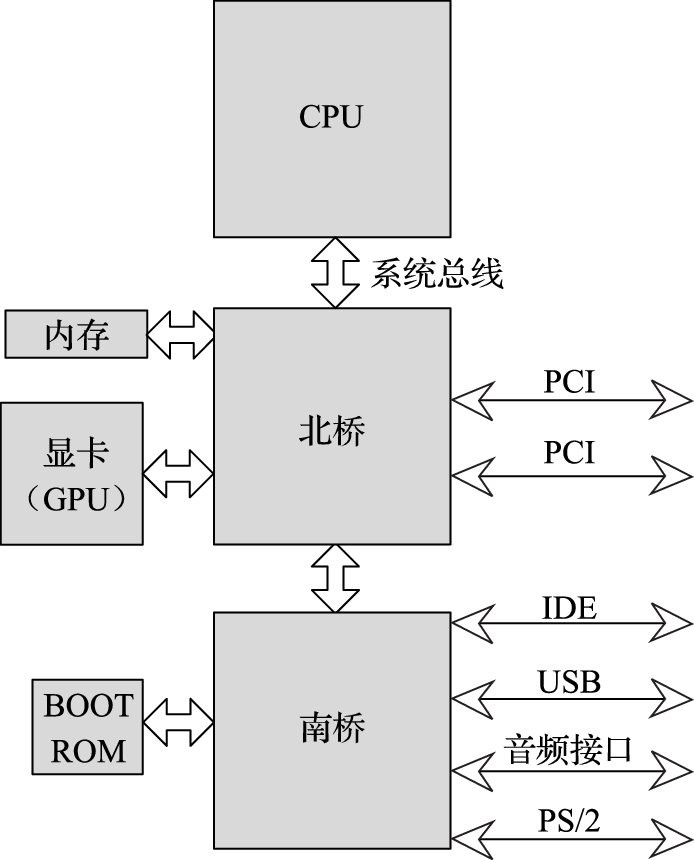
\includegraphics[width=0.5\linewidth]{assets/01/structure_4part.png}
  \caption{CPU-GPU-北桥-南桥结构}
  \label{fig:structure-4part}
\end{figure}

以英特尔奔腾处理器搭配的430HX芯片组为例，该芯片组采用了这种四片结构。其北桥芯片使用82439HX，南桥芯片采用82371SB，通过PCI总线扩展外接显卡，形成一个包括处理器在内的四片结构，构成计算机系统的核心部分。

\subsection{现代处理器 SoC 系统}\label{sec:01-overview-003}

片上系统（System on Chip，简称SoC）是一种单片计算机系统解决方案，它在单个芯片上集成了处理器、内存控制器、GPU以及硬盘、USB、网络等I/O接口，使得用户搭建计算机系统时只需使用单个主要芯片即可。SoC单片结构如图\ref{fig:soc}所示。

\begin{figure}[htbp]
  \centering
  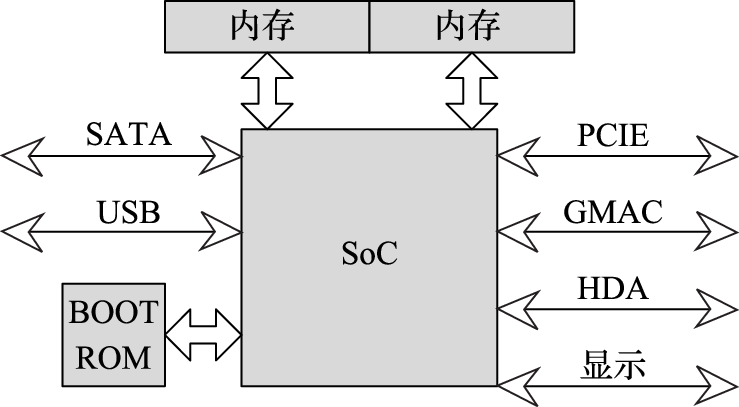
\includegraphics[width=0.5\linewidth]{assets/01/soc.png}
  \caption{SoC单片结构}
  \label{fig:soc}
\end{figure}

目前，SoC主要应用于移动处理器和工业控制领域。相比多片结构，单片SoC结构的集成度更高，功耗控制更加灵活，有利于系统的小型化和低功耗设计。然而，由于所有系统组件都集成在一个芯片上，SoC的系统扩展性较差，升级成本较高。随着技术的发展，封装基板上的互连技术不断进步，越来越多的处理器利用多片封装技术在单个芯片上集成多个硅片，以扩展芯片的计算能力或I/O能力。例如，AMD Ryzen系列处理器通过在封装上集成多个处理器硅片和I/O硅片，以提供针对不同应用领域的计算能力。龙芯3C5000L处理器则通过在封装上集成4个4核龙芯3A5000硅片，实现单片16核结构。

目前，主流商用处理器中，面向中高端领域的处理器普遍采用两片结构，而面向中低端及嵌入式领域的处理器则普遍采用单片结构。SoC单片结构最常见于手机等移动设备中。

\subsection{CPU芯片设计}\label{sec:01-overview-004}

在设计一款简单的现代系统级芯片（SoC）的过程中，一般需要达成以下核心目标：

\begin{enumerate}
\def\labelenumi{\arabic{enumi}.}
\tightlist
\item
  \textbf{处理器核心设计}
\end{enumerate}

\begin{itemize}
\tightlist
\item
  \textbf{架构选择}：一般选择一种简化的RISC（精简指令集计算）架构，如LoongArch精简指令集架构。该架构以其简单、高效和自主性著称，适合用于教育、研究和嵌入式系统。
\item
  \textbf{流水线技术}：采用流水线设计，以提高指令执行速度。流水线可以让处理器在一个周期内处理多条指令，提高吞吐量。
\item
  \textbf{缓存优化}：集成一级指令缓存（L1 I-cache）和数据缓存（L1 D-cache），以减少内存访问延迟，提高性能。
\item
  \textbf{虚拟地址翻译}：为支撑操作系统和应用程序的运行，设计虚拟地址翻译机制，支持虚拟内存管理。
\end{itemize}

\begin{enumerate}
\def\labelenumi{\arabic{enumi}.}
\setcounter{enumi}{1}
\tightlist
\item
  \textbf{外设设计}
\end{enumerate}

\begin{itemize}
\tightlist
\item
  \textbf{输入输出接口}：需要支持包括多种常见的I/O接口，如UART、SPI、I2C、GPIO等，确保与外部设备的兼容性和互操作性。
\item
  \textbf{内存控制器}：集成内存控制器，选择性支持SDRAM、DDR等类型内存，确保高效的数据存取。
\item
  \textbf{图形处理器}：集成简单的图形处理器，支持基本的图形处理需求，以提高用户体验。
\end{itemize}

\begin{enumerate}
\def\labelenumi{\arabic{enumi}.}
\setcounter{enumi}{2}
\tightlist
\item
  \textbf{系统互连}
\end{enumerate}

\begin{itemize}
\tightlist
\item
  \textbf{总线架构}：采用AMBA（Advanced Microcontroller Bus Architecture）等高效的总线架构，确保处理器核心和外设之间的高效数据传输。
\item
  \textbf{DMA控制器}：集成DMA控制器，支持大块数据的高速传输，减轻处理器核心的负担，提高系统整体效率。
\end{itemize}

\section{芯片实现流程简介}\label{sec:01-overview-005}

芯片实现流程是一系列复杂步骤的集合，包括从定义到设计再到物理实现、流片、封装、系统搭建等，涵盖了从概念到最终产品的转变。本节主要从流程的角度去概要性的描述如何实现CPU从概念提出到具体应用落地，整体流程示意如图\ref{fig:chip-flow1}所示，可分为前端设计与综合实现、后端物理实现与验证、流片制造与测试三个部分。需要注意的是如果在某个验证环节（比如功能仿真）没有通过，则需要回到前面设计（HDL设计或后端布局布线设计等）的某一步重新执行。下面针对这三个部分展开介绍。

\begin{figure}[htbp]
  \centering
  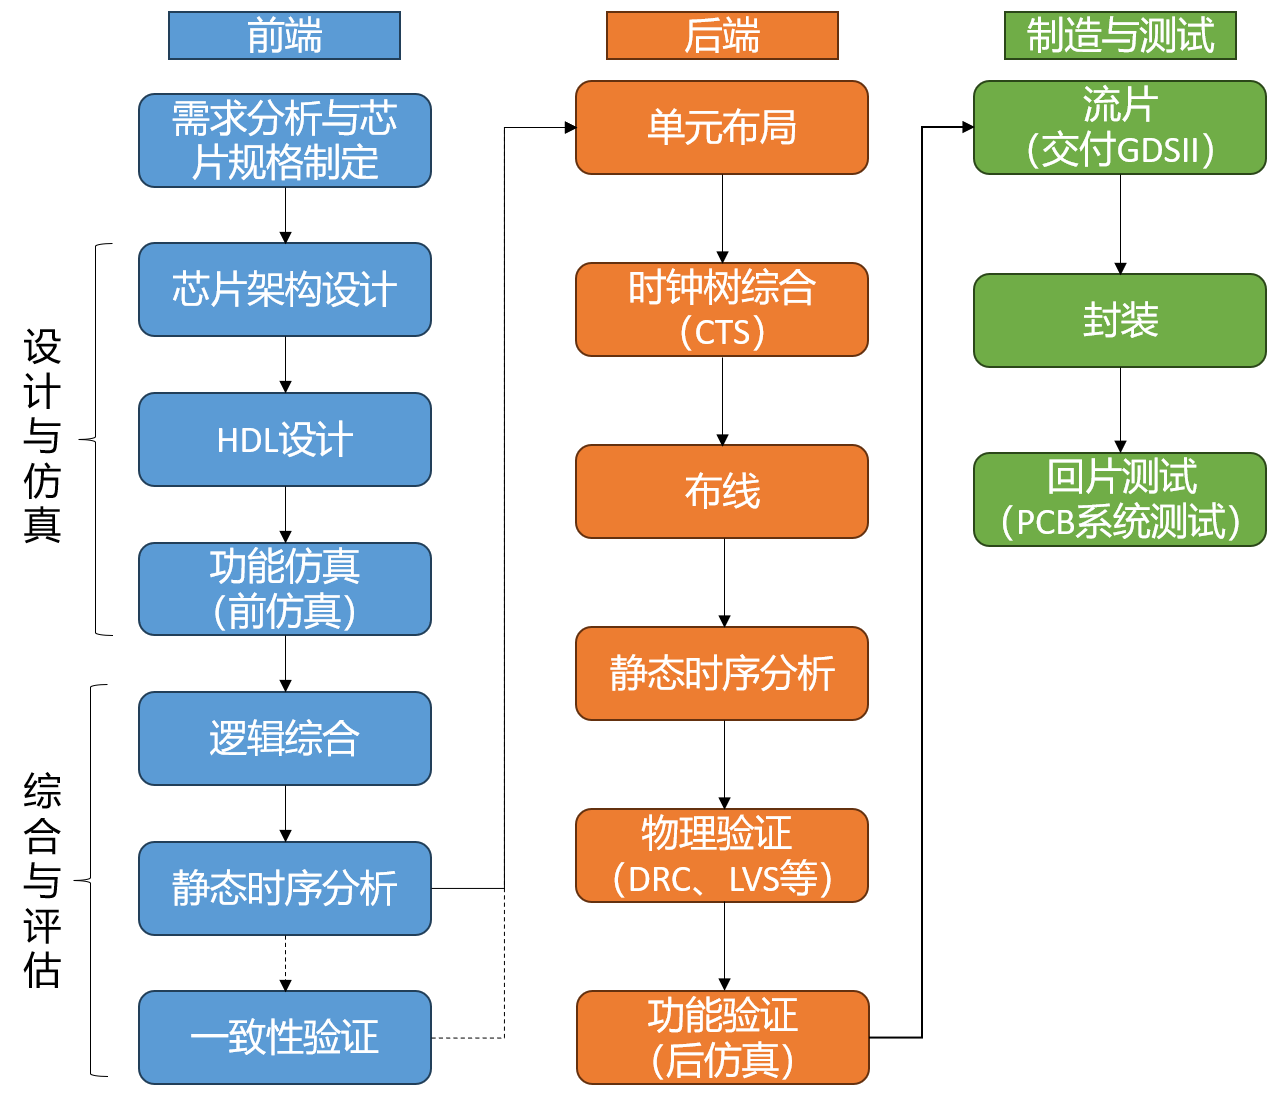
\includegraphics[width=0.5\linewidth]{assets/01/芯片实现流程.png}
  \caption{芯片实现流程示意图}
  \label{fig:chip-flow1}
\end{figure}

\subsection{芯片规格定义与设计仿真实现}\label{sec:01-overview-006}

首先芯片实现需要完成设计部分：

\begin{itemize}
\tightlist
\item
  \textbf{需求分析与规格制定}：首先一款处理器芯片，需要明确其应用场景，根据场景来确定需求，完成整体设计规格书（SPEC）。比如应用在嵌入式的处理器与应用在服务器的处理器二者对于性能、功能场景的需求差异就比较大。因此需要进行需求分析与规格制定。
\item
  \textbf{芯片架构设计}：一般对于大型负责芯片项目设计（比如现代CPU），都会在详细设计前进行系统架构设计。通过System C、Matlab等工具完成对架构的分析与验证，以确保在系统架构上不出现问题。
\item
  \textbf{HDL设计}：即通过硬件描述语言将所设计的架构进行实现。这一步一般通过VerilogHDL或VHDL来进行编写。需要注意的是此时编写的代码必须是可综合的RTL代码。目前也有一些其他更高级、敏捷的硬件描述语言在推广中，如chisel、SpinlHDL等，这些语言抽象层级更高，实现起来更加便捷。本教材中的部分CPU设计内容就是通过chisel来实现的。
\item
  \textbf{功能仿真}：此时也叫前仿真。即在HDL编写完成后需要进行仿真验证。这一步一般通过编写testbench，使用EDA仿真工具完成。当然在模块化设计的过程中，一般会每实现一个模块就要进行一次仿真，并根据仿真发现的问题进行修改设计中的错误。因此HDL设计与功能仿真这两步一般也可以放在一些来统称为HDL实现。在一些大型芯片项目中，仿真验证工作是占用时间最长的一部分。
\end{itemize}

在功能仿真完全正确之后，可以进行下一步，逻辑综合。

\subsection{芯片设计逻辑综合与评估验证}\label{sec:01-overview-007}

前面几步都属于设计的部分，本教材也着重讲述CPU设计部分的内容。在设计完成后，并不意味着能够将硬件代码完全冻结（即不再对HDL代码进行更改），因为时序等还没有进行收敛测试。下面进行几步来完成此事：

\begin{itemize}
\tightlist
\item
  \textbf{逻辑综合}：这一步主要是将HDL编写的RTL代码映射为可用于后端过程的门级网表。这一过程旨在决定电路的门级结构，寻求时序与面积以及功耗的平衡，同时增强电路的测试性。从这一步开始到后面的内容都将有具体工艺的参与。
\item
  \textbf{静态时序分析}：这一步主要用于分析电路时序是否满足要求，是用于时序signoff的关键步骤。一般EDA在进行逻辑综合时，也会进行一些静态时序分析（STA），但其准确性一般不如专门做STA的工具Synopsys PrimeTime工具。通过静态时序分析来分析电路的关键路径，分析硬件设计是否满足时序要求。若不满足则需要返回到HDL设计，通过针对关键路径优化等策略使时序收敛。
\item
  \textbf{一致性验证}：该步骤主要用于验证综合后的网表文件与综合前的HDL设计文件的功能一致性，以保证逻辑综合过程没有改变HDL所描述的电路功能。
\end{itemize}

在通过静态时序分析以及通过其他约束条件下收敛之后，网表文件就可以传递到下一步进行后端操作。

\subsection{芯片后端物理实现与验证}\label{sec:01-overview-008}

芯片后端物理实现主要包括布局规划、电源规划、时钟树综合、布线等步骤。验证包括芯片静态时序分析、功耗验证、物理验证等过程。

\begin{itemize}
\tightlist
\item
  \textbf{单元布局}：主要作用是将设计好的网表文件进行单元器件的摆放，一般布局包括布局规划、电源规划以及自动布局等步骤。布局规划即芯片尺寸规划、IO规划、macro摆放、物理单元插入等步骤。电源规划即将电源模块进行位置规划。自动布局即在完成规划的基础上，由EDA工具自动进行布局操作，以满足设定的时序、功耗、面积等条件或进行相应的优化。
\item
  \textbf{时钟树综合}：时钟树综合（CTS）是在物理设计中为芯片中的时钟信号构建一棵优化的树状结构，确保时钟信号能够同时到达所有时序单元，最小化时钟偏移和抖动，优化时序和功耗，从而确保芯片的时序收敛性和整体性能。
\item
  \textbf{布线}：一般分为全局布线与详细布线、布线优化等步骤。全局布线是指在芯片的全局范围内确定信号的布线路径和大致走线方向；详细布线是在全局布线的基础上，为每一根信号线分配具体的布线层、布线路径和布线宽度；在完成初步的详细布线后，进行布线优化以改善时序、降低功耗、减少信号干扰和提高芯片的制造良率。布线过程一般是EDA自动完成的，但有些情况可能需要手动布线。
\item
  \textbf{静态时序分析}：此时的时序分析有了更准确的单元延迟结果，此时的分析结果是更加精准的。这一步也用于芯片的时序signoff。
\item
  \textbf{物理验证}：主要验证设计规则检查（DRC）、电气规则检查（ERC）、布局与布线等效性验证（LVS）、信号完整性检查（SI）、功耗分析（Power Analysis）等。这些验证内容涵盖了从物理布局到电气性能的各个方面，确保芯片在功能、性能、制造和可靠性上都能达到预期要求。通过全面的物理验证，可以大大降低芯片流片失败的风险，确保芯片能够顺利进入量产阶段。
\item
  \textbf{功能验证}：这一步主要用于在版图实现后对电路功能的测试，这一步的测试条件就变得更加苛刻。再完成上述所有内容之后，后端就产出了GDSII文件用于发送给晶圆厂用于制造。
\end{itemize}

\subsection{芯片流片、封装与回片测试}\label{sec:01-overview-009}

一般芯片在回片前就需要完成对PCB测试系统的搭建。

\begin{itemize}
\tightlist
\item
  \textbf{流片制造}：在正式流片前，设计团队和客户要对设计进行最终签核（Sign-off），确保所有的设计规则、时序、信号完整性等问题都已经解决；制造厂根据设计文件制作光罩（mask），使用光罩在晶圆上进行光刻、刻蚀、掺杂、金属化等步骤，逐步将设计实现为物理晶体管、互连和其他器件。最终完成一款裸片（Die）的制造。
\item
  \textbf{芯片封装}：封装是指将制造完成的裸片（Die）进行物理保护并提供电气连接的过程。封装后的芯片可以安装到电路板上并与外部环境进行交互。一般封装会经过晶圆切割、晶圆测试、贴片封装、引线键合、倒装芯片（可选）、封装密封、测试、打标检查等步骤，最终出货给客户。
\item
  \textbf{测试系统搭建}：一般芯片完成封装后需要搭建测试系统来完成最终的功能、性能测试。包括外围电路设计、外设搭建、PCB绘制等。有时也会在回片前使用一个FPGA来模拟芯片功能进行系统的测试。
\item
  \textbf{芯片系统测试}：通过将芯片安装在测试电路板上，实现板上测试，最终验证芯片的功能、性能等特征。
\end{itemize}

通过以上介绍，完成了对一般数字芯片从设计到后端实现再到制造、回片测试各个环节的介绍。本教材将带领读者学习CPU芯片从架构设计到验证再到实现的各个细节，以真正让读者全面了解与掌握整个CPU芯片实现从理论到实践的核心知识。无论是初学者还是具有一定经验的工程师，本书都将提供系统的指导和实用的技巧，助力在CPU芯片设计过程中实现创新与突破。

% !TeX root = ../main.tex
% 原始章节：02-design-env.Rmd

\chapter{设计环境介绍}\label{chap:02-design-environment}

\section{硬件设计与验证环境}\label{sec:02-design-environment-001}

\subsection{FPGA原理介绍}\label{sec:02-design-environment-002}

FPGA（Field-Programmable Gate Array，现场可编程门阵列）是一种集成电路（IC）技术，其原理和传统的ASIC（Application-Specific Integrated Circuit，专用集成电路）有所不同。ASIC是预先设计好的、固定功能的集成电路，适合于大批量生产，但设计周期长且成本高。相比之下，FPGA是一种可编程的硬件，可以根据需要进行现场编程和配置，灵活性更高。

具体而言，FPGA具有如下特点：

\begin{enumerate}
\def\labelenumi{\arabic{enumi}.}
\item
  逻辑单元和可编程连接：FPGA由大量的可编程逻辑单元（Lookup Tables，LUTs）组成，这些LUTs可以实现各种逻辑功能。逻辑单元通过可编程的连接网络（可编程互连网络）互相连接，形成复杂的逻辑电路。
\item
  可编程的逻辑功能：FPGA支持可编程逻辑单元，允许设计者根据特定应用需求编写硬件描述语言（如Verilog或VHDL）代码，并将其编译成FPGA可执行的配置文件。这使得FPGA可以在运行时重新配置，从而实现不同的硬件功能，如数字信号处理、通信协议处理、图像处理等。
\item
  配置存储和编程：FPGA内部有配置存储器（Configuration Memory），用于存储设计者编写的硬件描述语言代码生成的配置信息。FPGA通常需要一个初始化文件（Bitstream），通过这个文件将设计好的逻辑配置加载到FPGA芯片中，完成硬件逻辑的配置。
\item
  时序管理和资源分配：设计FPGA时需要考虑时序管理，确保逻辑电路在时钟周期内正常工作。FPGA资源（如LUTs、片上存储器、DSP块等）在设计中需要合理分配和利用，以达到最佳性能和功耗平衡。
\item
  应用领域：FPGA广泛应用于需要高度定制化和灵活性的领域，如嵌入式系统、数字信号处理、网络处理、图像处理、加密解密等。它们也常用于快速原型设计和小批量生产，因为可以在设计后快速修改和优化硬件功能。
\end{enumerate}

\subsection{FPGA厂商简介}\label{sec:02-design-environment-003}

Xilinx 和 Altera（现在被Intel收购）是两大主要的FPGA厂商。

Xilinx FPGA常用的架构系列包括Spartan、Artix、Kintex和Virtex系列，每个系列适用于不同的应用需求和性能级别。Xilinx的关键技术包括可编程逻辑单元（LUTs）、DSP块、片上存储器等。
工具链方面，Xilinx提供的设计工具主要是Vivado Design Suite，用于设计、验证、综合和实现FPGA设计。其市场定位是通信、数据中心加速、视频处理、汽车电子等领域，特别擅长高性能和低功耗设计。

Altera的主要FPGA系列包括Cyclone、Arria和Stratix系列，每个系列也具有不同的性能等级和功能组合。
其设计工具是Quartus Prime，类似于Xilinx的Vivado，用于整个FPGA设计流程的支持和管理。市场定位同样是通信、工业控制、军事应用等领域，特别强调低成本、低功耗和高集成度的设计。

总体而言，Xilinx和Altera在FPGA的架构设计上有一些差异，涉及到逻辑单元、DSP资源、片上存储器等的配置和组织方式。而Vivado（Xilinx）和Quartus Prime（Altera）虽然在功能上有所差异，但都提供了完整的设计流程支持，包括综合、布局布线和验证等。

\subsection{硬件设计环境整体情况}\label{sec:02-design-environment-004}

以下将以Artix-7 FPGA XC7A200T为例介绍典型的FPGA开发板硬件资源。资源方面，其具有：

\begin{itemize}
\item
  逻辑单元（Logic Cells，包含大量的可编程逻辑单元（LUTs），用于实现各种逻辑功能）: 215360
\item
  DSP资源（DSP Slices，内置数字信号处理器块，用于高性能的数字信号处理任务。）: 740
\item
  片上存储器（Memory，包括分布式RAM和块RAM，用于存储数据和配置信息。）: 13140
\item
  GTP 6.6 Gb/s Transceivers: 16
\item
  I/O资源（I/O Pins，提供丰富的输入输出引脚，支持各种外部设备和接口的连接。）: 500
\end{itemize}

可以看到，典型的开发板上通常会集成上述FPGA芯片，并提供一些资源：

\begin{enumerate}
\def\labelenumi{\arabic{enumi}.}
\tightlist
\item
  外部接口
\end{enumerate}

\begin{itemize}
\item
  GPIO：通用输入输出引脚，用于连接外部电路和传感器。
\item
  通信接口：如UART、SPI、I2C等，用于与其他设备进行通信。
\item
  存储器：包括DDR RAM用于高速数据存储，以及Flash存储器用于程序和配置文件存储。
\end{itemize}

\begin{enumerate}
\def\labelenumi{\arabic{enumi}.}
\setcounter{enumi}{1}
\tightlist
\item
  时钟资源
\end{enumerate}

\begin{itemize}
\tightlist
\item
  晶振和时钟管理：提供稳定的时钟源和时钟分配器，用于同步各个部分的操作。
\end{itemize}

\begin{enumerate}
\def\labelenumi{\arabic{enumi}.}
\setcounter{enumi}{2}
\tightlist
\item
  调试和连接
\end{enumerate}

\begin{itemize}
\item
  调试接口：如JTAG接口，用于FPGA的调试和编程。
\item
  电源管理：提供电源管理电路，以确保稳定的工作电压和电流。
\end{itemize}

\begin{enumerate}
\def\labelenumi{\arabic{enumi}.}
\setcounter{enumi}{3}
\tightlist
\item
  附件功能
\end{enumerate}

\begin{itemize}
\item
  用户按键和LED指示灯：用于简单的用户交互和状态指示。
\item
  LCD显示器接口：用于连接液晶显示屏显示信息。
\end{itemize}

\subsection{龙芯CPU设计与体系结构教学实验系统}\label{sec:02-design-environment-005}

综合完成后，需要向FPGA烧录比特流，然后烧写Flash ROM，再通过串口观察输出，具体而言，需要提前准备龙芯FPGA开发板、FPGA电源线、FPGA下载线、Flash芯片、串口线、Vivado以及串口软件。

\begin{enumerate}
\def\labelenumi{\arabic{enumi}.}
\item
  Flash 芯片正确放置 FPGA 开发板上。
\item
  FPGA 开发板与电脑连接下载线、串口线。
\item
  电脑上打开 Vivado 工具中的 Open Hardware Manager，打开串口软件。
\item
  FPGA 板上电，如正常下载 bit 流文件一样下载 programmer\_by\_uart.bit 至 FPGA 上。
\item
  串口软件，波特率选为 230400。
\item
  串口连接正常后根据提示，键盘输入 x 表示开始 xmodem 传输。
\item
  串口软件使用 xmodem 模式传输 binary 文件。
\item
  等待传输完成。
\end{enumerate}

支持便完成了Flash ROM的烧写。特别地，对于其他类型的FPGA，可能没有对应的串口烧录比特率，此时则需要手动通过Flash烧录器对Flash进行烧录，烧录时需小心Flash芯片的摆放位置，以免烧坏芯片。

\section{软件调试环境}\label{sec:02-design-environment-006}

\subsection{RTL仿真验证介绍}\label{sec:02-design-environment-007}

在进行RTL设计时，通常需要进行仿真、验证和测试，以确保设计的正确性和功能性。仿真分为前仿真、后仿真。

前仿真是在逻辑综合（Synthesis）之前进行的仿真过程，主要用于验证RTL代码的功能和行为。前仿真通常使用的工具包括：

\begin{itemize}
\item
  Verilator：开源Verilog仿真器，用于对Verilog代码进行快速仿真和验证。通过将Verilog代码转换为C++代码，然后进行编译和仿真，能够提供较高的仿真速度和效率。
\item
  Vivado Simulator：Vivado Simulator是Xilinx Vivado工具套件中的一部分，用于Verilog和VHDL的仿真和验证。支持多种仿真模式和波形显示，适合对复杂的RTL设计进行验证和调试。
\end{itemize}

后仿真是在逻辑综合之后、实际FPGA或ASIC实现之前进行的仿真，目的是验证综合后的电路行为是否符合预期。后仿真使用的工具包括：

\begin{itemize}
\tightlist
\item
  VCS（Synopsys工具）：基于Verilog和VHDL的综合仿真工具，广泛用于后仿真和验证ASIC设计。提供了丰富的仿真和调试功能，支持高级优化和性能分析，适用于复杂的RTL设计和验证任务。
\end{itemize}

除了上述提到的Verilator、Vivado Simulator和VCS之外，还有一些其他常用的仿真工具：

\begin{itemize}
\item
  ModelSim：Mentor Graphics的仿真工具，支持Verilog、VHDL和SystemVerilog的仿真和调试。
\item
  Questa：Synopsys的仿真工具，也支持Verilog、VHDL和SystemVerilog，并提供了高级调试和分析功能。
\end{itemize}

\subsection{Vivado软件简介}\label{sec:02-design-environment-008}

如前面所述，Vivado是用于开发Vilinx FPGA的一款集成的EDA（Electronic Design Automation，电子设计自动化）软件工具，专门用于FPGA设计的各个阶段，包括仿真、综合（Synthesis）、布局布线（Implementation）以及验证。

作为综合的EDA工具链，Vivado提供了完整的EDA工具链，涵盖了FPGA设计流程中的各个关键步骤，从设计的初始阶段到最终的实现和验证。设计者可以使用Vivado进行前端设计，包括硬件描述语言（如Verilog、VHDL）编写和逻辑设计。Vivado支持高级综合（High-Level Synthesis，HLS），可以从高级语言（如C、C++）自动转换为硬件描述。同时，Vivado还包含强大的仿真工具，用于验证设计的功能和时序正确性，确保设计符合预期的行为。

综合是将硬件描述语言代码转换为FPGA可配置的逻辑单元和连线的过程。Vivado的综合工具能够优化设计，提高性能并确保满足时序要求。
在综合阶段，设计者可以进行约束设置，以指导工具如何优化设计以满足时序和资源利用率的要求。

Vivado也具有芯片后端工具的功能，例如用于布局布线，负责将逻辑元素放置在FPGA芯片上，并创建物理布线，确保电路的时序和电气特性符合要求。

\section{实验虚拟机}\label{sec:02-design-environment-009}

\subsection{实验虚拟机介绍}\label{sec:02-design-environment-010}

预装软件或环境：

\begin{itemize}
\tightlist
\item
  Vivado == 2019.2
\item
  VCS == 2018.09
\item
  Verdi2018 == 2018.06
\item
  chiplab == commit eb2a1eb479d89aa8382ec77f03473e1e2f0a6924
\item
  la32r编译工具链 == v0.0.3
\item
  verilator == v5.027
\item
  la32r-linux == v0.3
\item
  la32r-qemu == v0.0.2
\end{itemize}

\subsection{实验虚拟机获取}\label{sec:02-design-environment-011}

虚拟机获取链接：\url{https://pan.baidu.com/s/1CRMtk3d95JQnBx6FbHBWXA?pwd=chip}

\subsection{实验虚拟机安装}\label{sec:02-design-environment-012}

我们的虚拟机以OVF格式提供。下面介绍如何导入OVF。

\begin{enumerate}
\def\labelenumi{\arabic{enumi}.}
\tightlist
\item
  打开Vmware窗口
\item
  点击``文件''---``打开''，选择一个OVF文件，点击``打开''
\item
  输入OVF文件导入后的虚拟机名称、选择虚拟机的存放位置，点击``导入''
\item
  导入OVF文件需要较长的时间，请耐心等待，OVF文件导入后，就可以在虚拟机列表中看到OVF文件转换的虚拟机了
\item
  虚拟机用户\texttt{chip-env}的密码：\texttt{12345678}
\end{enumerate}

\subsection{实验代码仓库获取}\label{sec:02-design-environment-013}

\begin{itemize}
\tightlist
\item
  \href{https://github.com/BUAA-CI-LAB/BHLA.README}{北航龙架构处理器芯片敏捷设计框架（BHLA）}
\item
  \href{https://gitee.com/loongson-edu}{龙芯教育提供的相关资料}
\end{itemize}

% !TeX root = ../main.tex
% 原始章节：03-digital-logic.Rmd

\chapter{数字逻辑设计基础}\label{chap:03-digital-logic}

\section{设计与开发基本流程}\label{sec:03-digital-logic-001}

\subsection{数字电路的基本组成}\label{sec:03-digital-logic-002}

数字逻辑电路可以被划分为``组合逻辑电路''与``时序逻辑电路''两类。组合逻辑电路由逻辑门（如与门、或门、非门）组成，其输出完全取决于其当前的输入。而时序逻辑电路是利用组合逻辑电路和被称为``触发器（flip-flop）''的存储元件构建的，触发器可以将电路当前周期的状态缓存到下一个周期，因此时序逻辑电路的输出在任何时候都由当前输入组合和当前电路中触发器所保存的状态决定。

\subsubsection{组合逻辑电路}\label{sec:03-digital-logic-003}

组合逻辑电路是使用 AND、OR、NOT、NAND、NOR 等逻辑门搭建的。由于这些逻辑门仅根据当前的输入来产生输出，因此它们所组成的组合逻辑电路的输出也只根据当前的输入决定。

多路复用器（Multiplexer, 简称MUX）是一种重要的组合逻辑电路，它能够在多个输入信号中选择一个信号作为输出。多路复用器通常用于数据选择等场合，本节通过讲解多路复用器，来让读者对组合逻辑电路有一个直观的认识。一个典型的多路复用器具有以下三个主要部分：

\begin{itemize}
\item
  \textbf{输入信号}：多路复用器通常有多个输入信号通道，例如，一个2:1多路复用器有2个输入通道，4:1多路复用器有4个输入通道，以此类推。输入信号通道的数量通常是2的幂次，如2、4、8、16等。
\item
  \textbf{选择信号}：选择信号决定了从哪一个输入通道选择信号输出。选择信号的位数与输入信号的数量有关，例如，对于4:1多路复用器，需要2位选择信号；对于8:1多路复用器，需要3位选择信号。
\item
  \textbf{输出信号}：多路复用器有一个输出信号，输出信号由选择信号确定的输入信号所控制。
\end{itemize}

多路复用器通过选择信号的组合来选择相应的输入信号并将其传输到输出端。具体来说，对于一个 n:1 的多路复用器，存在 \(2^n\)\hspace{0pt} 个输入信号和 n 个选择信号，输出信号可以表示为一个函数：
\[
Y = MUX(I_0,I_1,...I_{2^n-1},S)
\]

例如，在一个4:1多路复用器中，有4个输入信号（\(I_0\),\$ I\_1\$, \(I_2\), \(I_3\)）和2位选择信号（\(S_1\), \(S_0\)），输出信号 Y 的表达式为：

\begin{itemize}
\tightlist
\item
  当 \(S_1,S_0=00\)时，\(Y=I_0\)\hspace{0pt}
\item
  当 \(S_1,S_0=01\)时，\(Y=I_1\)
\item
  当 \(S_1,S_0=10\)时，\(Y=I_2\)
\item
  当 \(S_1,S_0=11\)时，\(Y=I_3\)
\end{itemize}

多路复用器可以使用基本的逻辑门（如AND、OR、NOT）实现。以4:1多路复用器为例，其逻辑实现可以描述如下：
\[
Y = \overline{S_1} \cdot \overline{S_0} \cdot I_0 + \overline{S_1} \cdot S_0 \cdot I_1 + S_1 \cdot \overline{S_0} \cdot I_2 + S_1 \cdot S_0 \cdot I_3
\]
该表达式表明，输出信号\texttt{Y}是多个与门输出的逻辑或，每个与门对应一个输入信号和选择信号的组合。

\subsubsection{时序逻辑电路}\label{sec:03-digital-logic-004}

\textbf{时序逻辑电路}的输出不仅取决于当前的输入，还取决于电路的过去状态（历史输入）。时序逻辑电路通过存储元件来记忆过去的状态，因此具备状态记忆功能。典型的时序逻辑电路包括寄存器、计数器和移位寄存器等。

时序逻辑的基本原件包括触发器（Flip-Flops，简称FF）与锁存器（Latch）。触发器是时序逻辑电路的基本存储元件，用于存储一个比特的数据。常见的触发器类型包括D触发器、JK触发器、T触发器等。触发器的状态在时钟信号的上升沿或下降沿发生变化，因此触发器也被称为边沿触发器。锁存器与触发器相似，也是用于存储信息的元件，但其状态是在输入信号的电平触发下发生变化。常见的锁存器类型有SR锁存器和D锁存器。

D触发器是一种最常见的时序逻辑元件，用于存储一个比特的数据。它的工作特点是：在时钟信号的上升沿或下降沿（根据触发器类型）将输入数据（D）捕获并存储起来，直到下一次时钟触发时更新其输出状态。D触发器的主要输入包括：

\begin{itemize}
\tightlist
\item
  \textbf{D输入}：数据输入端，用于输入将要存储的数据。
\item
  \textbf{CLK}：时钟输入端，用于控制数据存储的时刻。D触发器在时钟信号的特定边沿（上升沿或下降沿）发生触发。
\item
  \textbf{Q输出}：输出端，存储的数据信号从该端输出。
\end{itemize}

在时钟信号（CLK）的上升沿（或下降沿，视具体设计而定），D触发器将D输入的数值捕获并存储。此时，输出Q与输入D同步。只要时钟信号没有再次触发，输出Q保持不变，维持之前存储的值。

数字电路中随处可见的\textbf{寄存器}就由多个D触发器组成，用于存储多位二进制数据。在时钟信号的控制下，输入的数据被同步存储在寄存器中，并在需要时输出。

\subsection{数字电路设计的基本流程}\label{sec:03-digital-logic-005}

数字电路设计是一个复杂而严谨的过程，通常分为五个主要步骤：电路设计、代码编写、功能仿真、综合实现和上板调试。这些步骤从概念到实际硬件实现，确保电路设计满足功能要求并在实际应用中稳定运行。

\subsubsection{电路设计}\label{sec:03-digital-logic-006}

\textbf{电路设计}是整个流程的第一步，旨在将系统的需求规格转化为具体的电路结构方案。这一过程包括以下几个关键步骤：

\begin{itemize}
\item
  \textbf{需求分析}：首先，设计者需要深入理解系统需求，明确电路需要实现的功能、性能指标、功耗要求等。需求规格通常包括逻辑功能描述、时序要求、输入输出规格、功耗限制等。
\item
  \textbf{设计分解}：在理解需求后，设计者将系统的整体需求分解成多个可管理的子模块。每个子模块负责实现特定的功能，多个模块间通过信号相互连接和交互。通过模块化设计，可以降低设计的复杂性，便于后续的调试和维护。
\item
  \textbf{电路结构设计}：设计者根据分解后的功能模块，构建电路结构图。这个步骤通常使用硬件描述语言（HDL）如Verilog或Chisel，或者使用电路图工具绘制草图。设计者需要考虑逻辑门、触发器、多路复用器、加法器等基本元件的使用。
\end{itemize}

\subsubsection{代码编写}\label{sec:03-digital-logic-007}

\textbf{代码编写}阶段将之前的电路设计方案转换为硬件描述语言（HDL）代码，以便在后续步骤中进行仿真和综合实现。具体包括：

\begin{itemize}
\tightlist
\item
  \textbf{HDL代码编写}：设计者使用Verilog、SystemVerilog、Chisel 等 HDL 语言，按照之前的电路结构图编写代码。每个模块的逻辑功能通过HDL代码描述，输入、输出信号以及逻辑操作在代码中详细定义。
\item
  \textbf{模块化设计}：代码编写时通常采用模块化设计，每个功能模块被定义为独立的代码段。这样便于代码的维护和重用，且提高了设计的可读性和调试的便利性。
\item
  \textbf{参数化设计}：为了增强设计的灵活性，设计者可能会使用参数化设计方法，在代码中引入参数，以便在不同条件下复用同一段代码。
\end{itemize}

\subsubsection{功能仿真}\label{sec:03-digital-logic-008}

\textbf{功能仿真}是数字电路设计中至关重要的步骤，通过软件仿真来验证设计的逻辑正确性，及时发现和修正潜在的错误。具体步骤包括：

\begin{itemize}
\tightlist
\item
  \textbf{测试平台搭建}：设计者搭建一个测试平台，模拟电路的工作环境，并为每个模块或整个系统编写测试用例。测试用例应覆盖各种正常和异常工作状态，以确保电路在所有可能的情况下都能正确工作。
\item
  \textbf{逻辑功能验证}：通过编译仿真软件（如 Verilator 或 Vivado），设计者编译运行HDL代码，查看仿真结果是否符合预期。如果仿真结果与预期不符，设计者需要回到代码编写阶段进行修改。
\item
  \textbf{时序分析}：在验证逻辑功能的同时，设计者还需进行时序分析，确保信号的传播延迟和时钟周期满足设计要求，防止时序错误。
\end{itemize}

\subsubsection{综合实现}\label{sec:03-digital-logic-009}

\textbf{综合实现}是将HDL代码转换为实际硬件电路的过程，主要分为两个子阶段：综合和实现。

\begin{itemize}
\tightlist
\item
  \textbf{综合}：在综合阶段，仿真通过的HDL代码被综合工具（如Xilinx的Vivado或Synopsys的vcs）转换为门级网表。这一阶段会对电路进行逻辑优化，包括减少门的数量、优化时序路径等。设计者需要检查综合报告，确保电路的逻辑功能和时序性能符合设计要求。
\item
  \textbf{实现}：实现阶段将门级网表映射到具体的硬件资源，如FPGA的查找表（LUT）、触发器、布线资源等。映射完成后，设计者需要进行布局布线，确保电路能够在芯片上正确实现。这一步骤生成的硬件设计文件将用于后续的硬件配置。
\end{itemize}

\subsubsection{上板调试}\label{sec:03-digital-logic-010}

\textbf{上板调试}是整个设计流程的最后一步，在这一阶段，设计者将生成的硬件设计文件下载到目标硬件平台（如FPGA开发板）上，进行实际的硬件测试和调试。具体过程包括：

\begin{itemize}
\tightlist
\item
  \textbf{硬件配置}：设计者将综合实现阶段生成的比特流文件或配置文件加载到FPGA芯片中，配置硬件资源以实现设计的逻辑功能。
\item
  \textbf{功能验证}：上板后，设计者通过各种测试手段（如示波器、逻辑分析仪）验证电路的功能和性能。测试可能包括对输入信号的激励测试、对输出信号的观察，以及对内部信号状态的分析。
\item
  \textbf{故障排查与修正}：如果上板调试过程中发现功能不符或性能问题，设计者需要分析问题来源，可能涉及硬件资源的限制、布线延迟过大等。问题修正后，设计者可能需要重新进行部分设计、综合和实现步骤。
\item
  \textbf{最终验证}：经过多次调试和修正，设计者最终确认电路在硬件上能稳定工作，并满足设计规格的所有要求。上板调试结束后，设计流程基本完成，设计者可以将电路投入实际应用。
\end{itemize}

\section{设计与调试方法}\label{sec:03-digital-logic-011}

在数字电路设计中，设计与调试方法的掌握对于最终电路的实现至关重要。本节将详细讨论设计与调试的关键步骤，从硬件基础知识入手，逐步讲解硬件描述语言编程、功能仿真、以及整体实现的流程与方法。

\subsection{硬件基础知识}\label{sec:03-digital-logic-012}

数字电路的设计基于一系列基础的硬件概念和元件。理解这些基础知识是成功设计和调试电路的前提条件。

\subsubsection{逻辑门}\label{sec:03-digital-logic-013}

\textbf{逻辑门}是数字电路的最基本构建块，通过它们可以实现所有的逻辑运算。常见的逻辑门包括：

\begin{itemize}
\tightlist
\item
  \textbf{与门（AND）}：输出只有在所有输入都为高电平（1）时为高电平，否则为低电平（0）。
\item
  \textbf{或门（OR）}：只要有一个输入为高电平，输出即为高电平；所有输入为低电平时，输出才为低电平。
\item
  \textbf{非门（NOT）}：它有一个输入和一个输出，输出与输入相反，即输入为1时输出为0，输入为0时输出为1。
\item
  \textbf{异或门（XOR）}：当输入的二进制数的1的个数为奇数时，输出为1；否则输出为0。
\end{itemize}

逻辑门通过组合可以构建更复杂的电路，如加法器、编码器、解码器、以及多路复用器等。

\subsubsection{触发器}\label{sec:03-digital-logic-014}

\textbf{触发器}是时序逻辑电路的核心元件，用于存储一个比特的数据。触发器的输出不仅依赖于当前输入，还依赖于先前的状态。常见的触发器类型包括：

\begin{itemize}
\tightlist
\item
  \textbf{D触发器}：在时钟信号的上升沿或下降沿，D触发器将输入D的值锁存到输出Q，直到下一个时钟信号的到来。
\item
  \textbf{JK触发器}：通过输入J和K信号，可以灵活地实现置1、置0和保持状态，是功能更为丰富的触发器。
\item
  \textbf{T触发器}：输入信号T为1时，输出状态在时钟信号的边沿发生翻转；T为0时，保持不变。T触发器常用于实现计数器。
\end{itemize}

\subsubsection{寄存器}\label{sec:03-digital-logic-015}

\textbf{寄存器}是一种存储器元件，用于存储二进制数据。在设计中，寄存器通常用于存储计算结果、状态信息或其他需要暂时保存的数据。

\begin{itemize}
\tightlist
\item
  \textbf{并行寄存器}：可以同时读取和写入多个比特数据。
\item
  \textbf{移位寄存器}：能够以时钟信号的驱动，将数据位按指定方向（左或右）移动。移位寄存器通常用于数据的序列传输或某些特定算法的实现。
\end{itemize}

\subsubsection{组合逻辑电路设计}\label{sec:03-digital-logic-016}

\textbf{组合逻辑电路}是指输出仅依赖于当前输入的电路，这类电路不具有记忆功能。设计组合逻辑电路通常需要以下步骤：

\begin{itemize}
\tightlist
\item
  \textbf{逻辑功能分析}：确定电路的功能需求，并使用真值表或布尔代数描述逻辑关系。
\item
  \textbf{逻辑表达式简化}：通过卡诺图（K-map）或布尔代数简化逻辑表达式，以减少逻辑门的数量。
\item
  \textbf{电路实现}：根据简化后的逻辑表达式设计逻辑门电路。
\end{itemize}

\subsubsection{时序逻辑电路设计}\label{sec:03-digital-logic-017}

\textbf{时序逻辑电路}则不仅依赖于当前输入，还依赖于电路的历史状态。时序逻辑电路具有存储功能，设计时需要考虑以下几个步骤：

\begin{itemize}
\tightlist
\item
  \textbf{状态分析与分解}：首先分析电路的工作状态，通常通过状态图或状态表描述各个状态之间的转换关系。
\item
  \textbf{状态编码}：为每个状态分配二进制编码，并确定状态转换的条件。
\item
  \textbf{逻辑实现}：根据状态图和状态转换条件，设计出相应的逻辑电路，包括组合逻辑和触发器的使用。
\end{itemize}

时序逻辑电路的应用包括有限状态机（FSM）、计数器、寄存器等，设计时必须考虑时钟信号的同步性和电路的时序性能。

\subsection{硬件描述语言编程}\label{sec:03-digital-logic-018}

在数字电路设计中，硬件描述语言（HDL）如Verilog HDL被广泛应用于电路的描述、仿真和综合。相比传统编程语言（如C语言），HDL的编写方法和语法有其独特之处。

\subsubsection{硬件描述语言简介}\label{sec:03-digital-logic-019}

硬件描述语言是一种专门用于描述数字电路结构和行为的编程语言。不同于软件编程语言，HDL描述的是并行操作、信号流动和时序逻辑。Verilog HDL是当前最流行的HDL之一，它的语法与C语言有一定相似之处，但其核心理念和应用场景完全不同。

\subsubsection{Verilog HDL的基本语法}\label{sec:03-digital-logic-020}

在Verilog HDL中，设计者可以通过模块（module）定义电路的结构。一个典型的模块包括输入、输出端口定义和逻辑描述。

\textbf{模块定义}：

% 代码语言：BookVerilog
\begin{CodeBlock}[language=BookVerilog]
module and_gate(
    input wire a,
    input wire b,
    output wire y
);
    assign y = a & b;
endmodule
\end{CodeBlock}

在上述代码中，\texttt{and\_gate}是一个简单的与门模块，通过\texttt{assign}语句将输入信号\texttt{a}和\texttt{b}的与运算结果赋值给输出\texttt{y}。

\textbf{时序逻辑描述}： 时序逻辑的描述通常使用\texttt{always}块来实现：

% 代码语言：BookVerilog
\begin{CodeBlock}[language=BookVerilog]
always @(posedge clk) begin
    q <= d;
end
\end{CodeBlock}

在这个代码片段中，\texttt{q}在时钟信号\texttt{clk}的上升沿时，接受输入\texttt{d}的值。这种描述方式使得Verilog可以精确模拟硬件电路的行为。

\subsubsection{Verilog HDL中的数据类型与操作}\label{sec:03-digital-logic-021}

Verilog HDL提供了丰富的数据类型与操作符，帮助设计者精确控制电路的行为。

\begin{itemize}
\tightlist
\item
  \textbf{数据类型}：常见的数据类型包括\texttt{wire}（导线）、\texttt{reg}（寄存器）等。\texttt{wire}通常用于组合逻辑，而\texttt{reg}用于时序逻辑。
\item
  \textbf{操作符}：Verilog支持各种逻辑操作符（如\texttt{\&}, \texttt{\textbar{}}, \texttt{\^{}}等）、算术操作符（如\texttt{+}, \texttt{-}, \texttt{*}等）、比较操作符（如\texttt{==}, \texttt{!=}等），以及位操作符（如\texttt{\textless{}\textless{}}, \texttt{\textgreater{}\textgreater{}}等），这些操作符使得电路的描述更加灵活。
\end{itemize}

\subsubsection{行为级描述与结构级描述}\label{sec:03-digital-logic-022}

Verilog HDL支持不同抽象层次的描述方法：

\begin{itemize}
\tightlist
\item
  \textbf{行为级描述}：侧重于电路的功能而非实现细节，通常用于仿真和验证。例如使用\texttt{always}块和\texttt{if-else}结构来描述复杂的逻辑行为。
\item
  \textbf{结构级描述}：侧重于电路的具体实现细节，通过实例化基本模块（如与门、或门）和连线来构建复杂电路，适合对电路结构有明确要求的设计。
\end{itemize}

\subsubsection{Verilog HDL编程的调试技巧}\label{sec:03-digital-logic-023}

在编写Verilog HDL代码时，调试是不可避免的一部分。常用的调试技巧包括：

\begin{itemize}
\tightlist
\item
  \textbf{仿真测试}：通过编写测试平台和测试用例，验证模块功能的正确性。常用的编译仿真工具有Verilator、Vivado等。
\item
  \textbf{代码覆盖率分析}：通过分析仿真过程中哪些代码段被执行，判断测试用例的全面性。
\item
  \textbf{波形分析}：仿真过程中生成的波形文件（如VCD文件）可以通过波形查看器观察信号的时序关系，帮助排查时序错误。
\end{itemize}

\subsection{功能仿真}\label{sec:03-digital-logic-024}

功能仿真是数字电路设计中验证电路逻辑功能的重要步骤。仿真环境的搭建和功能仿真软件的使用直接影响到电路设计的质量和效率。

\subsubsection{仿真环境的搭建}\label{sec:03-digital-logic-025}

仿真环境的搭建是进行功能仿真的第一步。一个完整的仿真环境通常包括以下几个部分：

\begin{itemize}
\tightlist
\item
  \textbf{仿真工具选择}：根据设计规模和需求选择合适的仿真工具，如Verilator、Vivado Simulator、Questa等。不同的工具提供的功能和接口各有特点，设计者可以根据需要选择合适的工具。
\item
  \textbf{仿真平台搭建}：仿真平台通常包括待测模块（DUT）、测试平台（Testbench）、输入信号生成器和结果比较器。Testbench是整个仿真环境的核心，它负责生成输入信号、接收DUT的输出，并与预期结果进行对比。
\item
  \textbf{输入信号生成}：根据电路的设计要求，生成各种输入信号以测试电路在不同情况下的行为。这些信号可以是简单的脉冲信号，也可以是复杂的波形数据，甚至是来自文件的真实数据。
\end{itemize}

\subsubsection{仿真测试策略}\label{sec:03-digital-logic-026}

为了确保电路设计的全面性和可靠性，仿真测试需要采用多种策略：

\begin{itemize}
\tightlist
\item
  \textbf{边界测试}：测试输入信号在边界条件下的行为，例如信号的最大值、最小值、零输入等。
\item
  \textbf{随机测试}：生成随机的输入信号，测试电路在非预期情况下的表现。这种方法有助于发现隐藏的设计错误。
\item
  \textbf{覆盖测试}：通过分析仿真过程中执行的代码段，确保所有可能的逻辑路径都经过测试。代码覆盖率是衡量测试全面性的重要指标。
\item
  \textbf{回归测试}：在每次设计修改后，重新运行所有测试用例，确保新的修改没有引入新的错误。
\end{itemize}

\subsection{整体实现}\label{sec:03-digital-logic-027}

在数字电路设计的最终阶段，设计者需要将设计的电路从仿真环境转移到实际硬件中。这一过程包括综合、实现、配置以及最终的硬件调试。以下是完整的CPU实现与调试流程的简要介绍。

\subsubsection{CPU设计概述}\label{sec:03-digital-logic-028}

CPU（中央处理单元）是复杂数字电路设计的典型代表，其设计包含指令集架构（ISA）的定义、数据路径的设计、控制单元的实现等。CPU的设计涉及到丰富的硬件知识，包括组合逻辑、时序逻辑、存储器、寄存器和总线系统等。

\subsubsection{综合（Synthesis）}\label{sec:03-digital-logic-029}

综合是将HDL代码转化为门级网表的过程。在这一过程中，综合工具会根据目标硬件的特性，优化HDL代码，并生成实际硬件所需的逻辑门电路。综合报告提供了电路的关键路径、功耗分析、时钟频率等信息。

\begin{itemize}
\tightlist
\item
  \textbf{逻辑优化}：在综合过程中，工具会自动对电路进行优化，如去除冗余逻辑、优化组合逻辑路径等，以提高电路的性能。
\item
  \textbf{约束设置}：设计者需要在综合前设置时序约束、功耗约束等参数，确保综合后的电路能在目标硬件上正常工作。
\item
  \textbf{门级仿真}：综合完成后，设计者可以对门级网表进行仿真，确保逻辑功能在优化后的电路中保持一致。
\end{itemize}

\subsubsection{实现（Implementation）}\label{sec:03-digital-logic-030}

实现阶段包括映射、布局布线、时序分析等步骤，将综合生成的门级网表转换为具体的硬件配置文件。

\begin{itemize}
\tightlist
\item
  \textbf{映射（Mapping）}：将逻辑门级网表映射到目标硬件的基本单元（如LUT、触发器等）。映射过程中的资源分配直接影响到电路的性能和面积。
\item
  \textbf{布局布线（Place \& Route）}：布局布线是将电路中的逻辑单元分配到硬件的具体位置，并为它们之间建立连线。这一步骤直接影响电路的时序性能，特别是在高速设计中尤为重要。
\item
  \textbf{静态时序分析（STA）}：在布局布线完成后，设计者需要进行静态时序分析，检查电路的时序是否满足设计要求，如时钟频率、信号传播延迟等。
\end{itemize}

\subsubsection{上板测试与调试}\label{sec:03-digital-logic-031}

在生成最终的硬件配置文件后，设计者将其下载到目标硬件（如FPGA开发板）上进行实际测试。

\begin{itemize}
\tightlist
\item
  \textbf{硬件下载与配置}：通过JTAG或其他下载工具，将配置文件加载到硬件平台。配置完成后，硬件电路开始运行，设计者可以通过观察输出信号或使用调试工具验证电路的功能。
\item
  \textbf{功能验证}：在硬件上运行设计的测试用例，验证电路的功能和性能是否符合预期。设计者可以通过逻辑分析仪、示波器等工具进行深入的信号分析。
\item
  \textbf{问题分析与修正}：如果测试结果与预期不符，设计者需要分析硬件上的问题来源，可能涉及信号干扰、时序错误、功耗超标等因素。解决这些问题可能需要回到设计的早期阶段进行调整，然后重新综合和实现。
\item
  \textbf{最终调优}：经过多次调试后，设计者对电路进行最终调优，确保其在硬件上能够稳定、高效地运行。调优可能涉及调整时钟频率、优化电路路径、调整功耗分配等。
\end{itemize}

\subsubsection{项目交付}\label{sec:03-digital-logic-032}

在CPU设计和调试完成后，设计者通常需要准备项目交付文档。这些文档包括设计规范、测试报告、硬件配置文件、时序分析报告等。项目交付文档不仅为后续的维护和升级提供了参考，也为最终用户提供了操作指导和技术支持。

\section{相关工具与平台介绍}\label{sec:03-digital-logic-033}

以下列出了一些常用的工具和平台，帮助学习和实践数字逻辑设计：

\begin{itemize}
\item
  HDLBits：HDLBits 是一个用于学习硬件描述语言（主要是 Verilog）和数字逻辑设计的在线平台。该平台由加拿大多伦多大学创建，主要用于教学目的。HDLBits 提供了大量的练习题，涵盖了从基础到高级的数字逻辑设计概念，如基本门电路、组合逻辑、时序逻辑、状态机等。
\item
  FPGA Design Elements：FPGA Design Elements 是一个数字设计的在线资源，专注于 FPGA 设计的各个方面。该平台包含了丰富的设计实例、教程和工具，帮助设计者更好地理解和实现 FPGA 上的数字电路。
\item
  Xilinx Vivado：Xilinx 提供的综合开发环境，用于 FPGA 设计，支持 Verilog 和 VHDL 语言。
\item
  Intel Quartus：Intel 的 FPGA 设计软件，提供了综合、时序分析和硬件调试工具。
\item
  ModelSim：广泛使用的 HDL 仿真工具，支持 Verilog 和 VHDL 语言，适用于设计验证。
\item
  Simulink：MATLAB 的附加工具，用于数字电路的图形化设计与仿真，适合于较高层次的系统设计。
\item
  Yosys：开源综合工具，用于 Verilog HDL 的 RTL 设计综合。
\end{itemize}

% !TeX root = ../main.tex
% 原始章节：04-toolchain.Rmd

\chapter{数字电路设计训练}\label{chap:04-toolchain}

\section{LoongArch指令集32位精简版（LA32R）介绍}\label{sec:04-toolchain-001}

\subsection{指令集介绍}\label{sec:04-toolchain-002}

LoongArch是由龙芯中科自主研发的指令集架构，于2020年8月13日首次公开。其拥有基础指令、虚拟化扩展、二进制翻译扩展、向量扩展、高级向量扩展等
近2000条原生指令，具有完全自主、技术先进、兼容生态三方面特点。

LoongArch为32/64位定长RISC指令集，支持多种指令格式，针对MIPS、ARM、x86等指令集架构支持高效的二进制翻译。当前，LoongArch指令集生态日益
丰富，基础软件方面支持龙芯浏览器、Java、Node.js、Python、Ruby等；工具链方面支持GNU编译工具链、LLVM编译器、Golang编译器、Rust编译器等；
云计算方面支持Kubernetes、Docker等；系统软件方面，Linux主线已支持LoongArch 32/64。

LoongArch 32位精简版是LoongArch指令集的子集，其拥有基础指令140条，主要用于体系结构教学。LoongArch 32位精简版包含算术运算、移位运算、
转移、普通访存、原子访存、栅障、基础整数杂项、浮点运算类、浮点比较、浮点转换、浮点搬运、浮点分支、浮点普通访存、CSR访问、Cache维护、
TLB维护、特权杂项等17种指令类型。存储支持直接地址翻译和映射地址翻译两种模式，在映射地址翻译模式下，还可以通过直接映射配置窗口机制（DMW）
完成虚实地址的直接映射；存储访问支持一致可缓存和强序非缓存两种类型。LA32R与LoongArch 32/64的关系如图\ref{fig:la-branch}所示。

\begin{figure}[htbp]
  \centering
  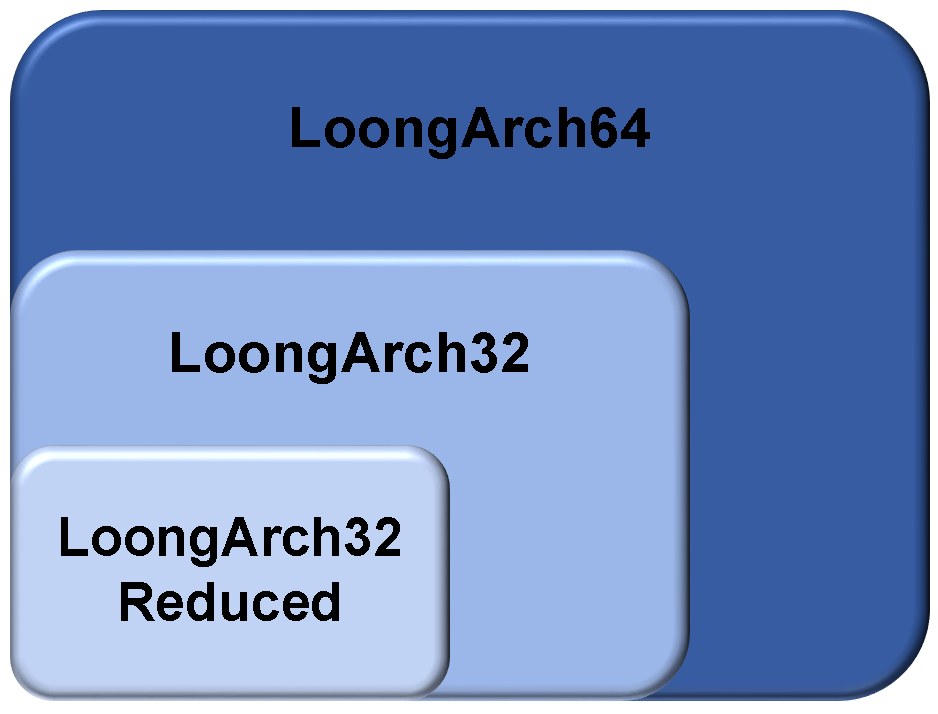
\includegraphics[width=0.5\linewidth]{assets/04/la-branch.png}
  \caption{龙架构的三个分支}
  \label{fig:la-branch}
\end{figure}

LoongArch 32位精简版支持例外和中断。中断采用线中断形式，每个处理器核内部可记录12个线中断，包括1个核间中断（IPI）、1个定时器中断（TI）、
8个硬中断（HWI0～HWI7）、2个软中断（SWI0～SWI1）。所有的线中断都是电平中断，且都是高电平有效。

例外包含中断（INT）、load操作页无效（PIL）、store操作页无效（PIS）、取指操作页无效（PIF）、页修改（PME）、页特权等级不合规（PPI）、
取指地址错（ADEF）、访存指令地址错（ADEM）、地址非对齐（ALE）、系统调用（SYS）、断点（BRK）、指令不存在（INE）、指令特权等级错（IPE）、
浮点指令未使能（FPD）、基础浮点指令例外（FPE）、TLB重填（TLBR）等16种例外。

龙架构具有较好的自主性、先进性与兼容性。龙架构从整个架构的顶层规划，到各部分的功能定义，再到细节上每条指令的编码、名称、含义，在架构上进行自主重新设计，
具有充分的自主性。龙架构摒弃了传统指令系统中部分不适应当前软硬件设计技术发展趋势的陈旧内容，吸纳了近年来指令系统设计领域诸多先进的技术发展成果。
同原有兼容指令系统相比，不仅在硬件方面更易于高性能低功耗设计，而且在软件方面更易于编译优化和操作系统、虚拟机的开发。

\subsection{指令编码格式}\label{sec:04-toolchain-003}

龙芯架构32位精简版中的所有指令均采用32位固定长度，且指令的地址都要求4字节边界对齐。当指令地址不对齐时将触发地址错例外。

指令编码的风格是所有寄存器操作数域都从第0比特开始从低到高依次摆放。操作码都是从第31比特开始从高到低依次摆放。如果指令中包含有立即数操作数，那么立即数域位于寄存器域和操作码域之间，根据不同指令类型有不同的长度。

具体来说,包含9种典型的指令编码格式,即3种不含立即数的编码格式2R、3R、4R,以及6种含立即数的编码格式2RI8、2RI12、2RI14、2RI16、1RI21、I26。表1-1列举了这9种典型编码格式的具体定义。

需要指出的是,存在少数指令,其指令编码域并不完全等同于这9种典型指令编码格式,而是在其基础上略有变化。不过这种指令的数目并不多,且变化的幅度也不大,不会对于编译系统的开发人员带来不便。

9种典型指令编码格式的定义如图\ref{fig:encoding-format}所示。

\begin{figure}[htbp]
  \centering
  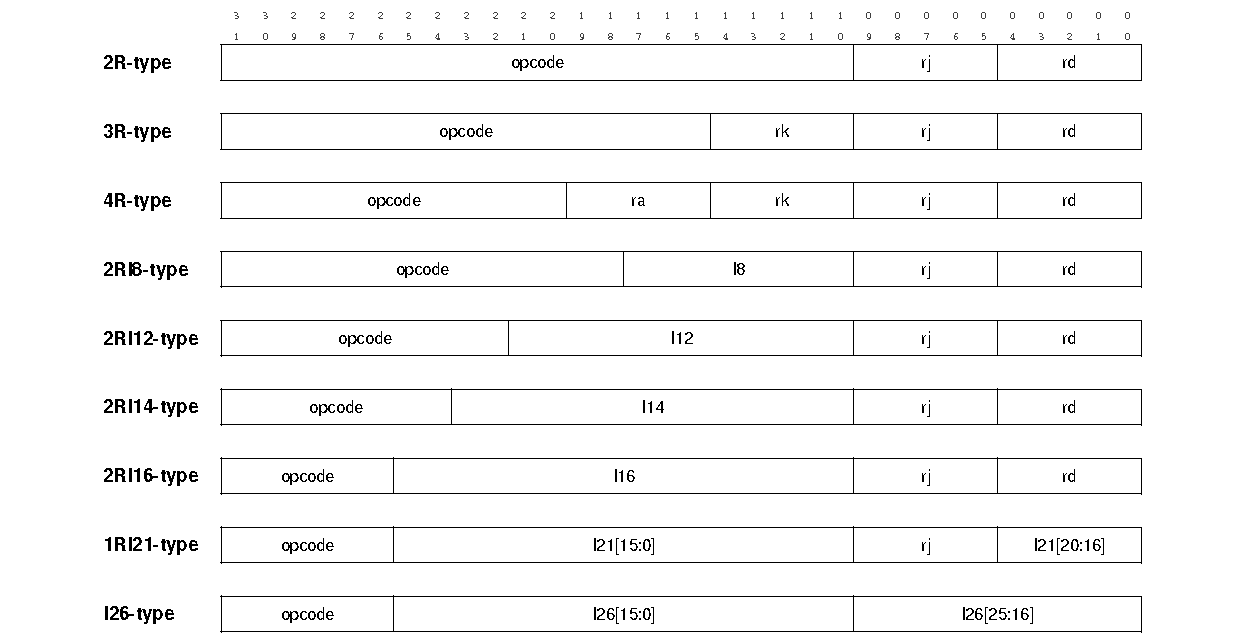
\includegraphics[width=1\linewidth]{assets/04/encoding-format.pdf}
  \caption{LA32R指令编码格式}
  \label{fig:encoding-format}
\end{figure}

\subsection{指令分类}\label{sec:04-toolchain-004}

LA32R指令集的指令类型可以分为以下几类：

\begin{itemize}
\item \textbf{整数分支跳转指令}：用于控制程序流的跳转和分支。
\item \textbf{整数计算指令}：用于进行各种整数运算。
\item \textbf{整数访存指令}：用于内存的读取和写入。
\item \textbf{特权指令集}：包括操作系统和硬件特权操作的指令。
\item \textbf{浮点指令集}：虽然本节不展开详细介绍，但浮点指令集包括用于浮点运算的指令。
\end{itemize}


\subsection{指令助记符}\label{sec:04-toolchain-005}

在龙芯架构的32位精简版中，指令汇编助记格式主要包括指令名和操作数两部分，为方便汇编编程人员和编译器开发人员使用，采用了统一的前、后缀规则。

\begin{enumerate}
\def\labelenumi{\arabic{enumi}.}
\tightlist
\item
  \textbf{指令名前缀}：

  \begin{itemize}
  \tightlist
  \item
    所有非向量浮点数指令的指令名以字母``F''开头，以区分整数和浮点数指令。
  \end{itemize}
\item
  \textbf{指令名后缀}：

  \begin{itemize}
  \tightlist
  \item
    绝大多数指令通过``.XX''形式的后缀来指示指令的操作对象类型。
  \item
    整数类型操作对象的后缀：

    \begin{itemize}
    \tightlist
    \item
      \texttt{.B}：有符号字节
    \item
      \texttt{.H}：有符号半字
    \item
      \texttt{.W}：有符号字
    \item
      \texttt{.BU}：无符号字节
    \item
      \texttt{.HU}：无符号半字
    \item
      \texttt{.WU}：无符号字
    \item
      注意：当操作数是否有符号不影响运算结果时，后缀不带``U''。
    \end{itemize}
  \item
    浮点数类型操作对象的后缀：

    \begin{itemize}
    \tightlist
    \item
      \texttt{.H}：半精度浮点数
    \item
      \texttt{.S}：单精度浮点数
    \item
      \texttt{.D}：双精度浮点数
    \item
      \texttt{.W}：有符号字
    \item
      \texttt{.WU}：无符号字
    \end{itemize}
  \end{itemize}
\item
  \textbf{无后缀情况}：

  \begin{itemize}
  \tightlist
  \item
    某些指令的操作对象数据位宽由处理器的实现（32位或64位）决定，例如SLT和SLTU指令。
  \item
    特权态指令（操作CSR、TLB和Cache）以及在不同寄存器文件之间移动数据的指令也不加后缀。
  \end{itemize}
\item
  \textbf{后缀组合}：

  \begin{itemize}
  \tightlist
  \item
    当源操作数和目的操作数的数据位宽和有无符号情况一致时，指令名只有一个后缀。
  \item
    如果源操作数数据位宽和有无符号情况一致，但与目的操作数不一致，指令名有两个后缀，第一个后缀表示目的操作数，第二个后缀表示源操作数。
  \item
    若源操作和目的操作数情况更复杂，指令名将按顺序列出目的操作数和每个源操作数的情况。
  \end{itemize}

  例如：

  \begin{itemize}
  \tightlist
  \item
    指令``MULW.D.WU rd, rj, rk''中：

    \begin{itemize}
    \tightlist
    \item
      \texttt{.D}对应目的操作数\texttt{rd}
    \item
      \texttt{.WU}对应源操作数\texttt{rj}和\texttt{rk}
    \item
      表示该乘法指令将两个无符号字相乘，结果是双字，写入\texttt{rd}中。
    \end{itemize}
  \item
    指令``CRC.W.B.W rd, rj, rk''中：

    \begin{itemize}
    \tightlist
    \item
      第一个\texttt{.W}对应\texttt{rd}
    \item
      \texttt{.B}对应\texttt{rj}
    \item
      第二个\texttt{.W}对应\texttt{rk}
    \item
      表示该CRC校验指令将\texttt{rj}中的字节消息与\texttt{rk}中的32位原校验值生成新的32位校验值，结果写入\texttt{rd}中。
    \end{itemize}
  \end{itemize}
\item
  \textbf{寄存器操作数}：

  \begin{itemize}
  \tightlist
  \item
    通用寄存器使用``rN''表示，其中N为寄存器编号。
  \item
    浮点寄存器使用``fN''表示，其中N为寄存器编号。
  \end{itemize}
\end{enumerate}

\section{LA32R指令集与MIPS指令集对比}\label{sec:04-toolchain-006}

\subsection{编码格式对比}\label{sec:04-toolchain-007}

LA32R与MIPS指令集（MIPS R4K）均为经典的RISC风格指令集，具有固定长度的指令格式。两者的编码格式存在一定差异。LA32R指令集采用了更丰富和清晰的指令编码格式，并且使用了前缀编码的技术。这使得LA32R在编码简洁性和灵活性方面优于MIPS。

\subsection{4.2.2 整数指令对比}\label{sec:04-toolchain-008}

在整数指令方面，LA32R相较于MIPS指令集有所简化。例如，LA32R没有HI/LO寄存器，也没有CLO/CLZ指令。LA32R还省略了xWL/xWR非对齐字访存指令。此外，LA32R的分支跳转指令没有延迟槽，并且立即数长度更长，使得跳转指令的执行更加高效和简洁。

\subsection{4.2.3 特权指令对比}\label{sec:04-toolchain-009}

在特权指令方面，LA32R与MIPS指令集有显著不同。LA32R在内存管理方面支持窗口映射和直接映射的机制，而MIPS则采用了固定窗口映射。LA32R简化了中断异常处理流程，并且在hazard控制方面相比MIPS进行了简化，使得处理器设计和实现更加高效。

\section{LA32R处理器开发工具流程}\label{sec:04-toolchain-010}

\subsection{Chiplab 验证环境介绍}\label{sec:04-toolchain-011}

chiplab项目是由龙芯提出，用于构建LA32R SoC的敏捷开发平台。其chip文件夹包含仿真/FPGA三套顶层SoC，IP文件夹放置SoC使用到的IP，包含处理器、SPI、Confreg等。

仿真的工作目录位于sims/verilator/run\_*，当前仅支持verilator。run\_prog : 该工作目录下可运行func测试用例、dhrystone、coremark性能测试程序、linux以及自定义C程序。run\_random : 该工作目录下可进行随机指令序列测试。

综合工作目录位于fpga，当前支持龙芯实验箱及百芯开发板。使用vivado打开loongson/20*.2/system\_run.xpr（根据具体vivado版本选择）或者Baixin/system\_run/system\_run.xpr工程文件，添加处理器核代码后，可直接开始综合。若选择添加chiplab中的参考核，注意添加myCPU/IP下的xilinx IP。
处理器核输入时钟频率默认为33MHz，可对clk\_pll\_33xilinx IP的输出时钟频率进行调整，修改处理器核的输入时钟频率。此外，还需将chip/soc\_demo/loongson/config.h或者chip/soc\_demo/Baixin/config.h文件中的FREQ宏定义修改为对应频率。

\subsection{Eula-Env 验证环境介绍}\label{sec:04-toolchain-012}

Eula-Env 项目是由北航百芯团队提供，致力于构建 LoongArch 32 Reduced 集成芯片敏捷开发平台，提供了全面的设计和测试框架。本节将介绍 Eula-Env 的功能。

Eula-Env 的文件结构如下：

\begin{itemize}
\tightlist
\item
  \texttt{am/}: 基于南京大学 AM 移植的 LoongArch 32 Reduced 裸机运行时环境
\end{itemize}

\begin{quote}
原仓库地址: \url{https://github.com/NJU-ProjectN/abstract-machine.git}
\end{quote}

\begin{itemize}
\item
  \texttt{eulacore}: 基于敏捷开发平台设计实现的九级顺序单发射处理器与 Verilator 仿真 SoC
\item
  \texttt{la32r-toolchains}: LoongArch 32 Reduced GNU 工具链和 newlib 链接库
\item
  \texttt{nemu}: 基于南京大学 NEMU 移植的 LoongArch 32 Reduced 仿真模拟器
\end{itemize}

\begin{quote}
原仓库地址: \url{https://gitee.com/wwt_panache/la32r-nemu.git}
\end{quote}

\begin{itemize}
\item
  \texttt{env.sh}: 环境变量加载脚本，需在编译程序前使用
\item
  \texttt{setup-tools.sh}: 依赖库/工具安装脚本
\item
  \texttt{setup.sh}: 一键配置脚本, 包含 env.sh 的功能, 初始化仓库子模块，并自动编译 nemu 与 am 中的 coremark 程序
\end{itemize}

通过 \texttt{setup.sh} 脚本，我们可以一键加载环境变量/编译 NEMU/编译 AM 的 Coremark 程序，而根据实际需求，我们可以逐一进行如下操作。

\begin{enumerate}
\def\labelenumi{\arabic{enumi}.}
\tightlist
\item
  加载环境变量
\end{enumerate}

% 代码语言：BookShell
\begin{CodeBlock}[language=BookShell]
$ source env.sh
\end{CodeBlock}

\begin{enumerate}
\def\labelenumi{\arabic{enumi}.}
\setcounter{enumi}{1}
\tightlist
\item
  编译行为仿真模型
\end{enumerate}

针对 CPU 设计的早期阶段，该项目设计了一套简易的 Verialtor 仿真 SoC，CPU 对外统一为一个 AXI4 接口，并通过 AXI4 转接桥连接 RAM、UART8250、Confreg，CPU具体定义如下图所示：

% 代码语言：BookVerilog
\begin{CodeBlock}[language=BookVerilog]
module mycpu_mega_top(
  input         clock,
  input         reset,
  input         awready,
  output        awvalid,
  output [31:0] awaddr,
  output [2:0]  awprot,
  output        awid,
  output        awuser,
  output [7:0]  awlen,
  output [2:0]  awsize,
  output [1:0]  awburst,
  output        awlock,
  output [3:0]  awcache,
  output [3:0]  awqos,
  input         wready,
  output        wvalid,
  output [31:0] wdata,
  output [3:0]  wstrb,
  output        wlast,
  output        bready,
  input         bvalid,
  input  [1:0]  bresp,
  input         bid,
  input         buser,
  input         arready,
  output        arvalid,
  output [31:0] araddr,
  output [2:0]  arprot,
  output        arid,
  output        aruser,
  output [7:0]  arlen,
  output [2:0]  arsize,
  output [1:0]  arburst,
  output        arlock,
  output [3:0]  arcache,
  output [3:0]  arqos,
  output        rready,
  input         rvalid,
  input  [1:0]  rresp,
  input  [31:0] rdata,
  input         rlast,
  input         rid,
  input         ruser,
  input  [7:0]  ext_int,
  output        global_reset
);
\end{CodeBlock}

为使得 CPU 接入该项目的 SoC，首先需要通过如下命令编译 SoC 仿真顶层模块，生成 SimTop.v 文件:

% 代码语言：BookShell
\begin{CodeBlock}[language=BookShell]
$ make verilog
\end{CodeBlock}

可以看到 SimTop.v 中包含了该项目的 SoC 顶层并实例化了 CPU 模块:

% 代码语言：BookVerilog
\begin{CodeBlock}[language=BookVerilog]
mycpu_mega_top core ( // @[EulaSimTop.scala 27:20]
   .awready(core_awready),
   .awvalid(core_awvalid),
   ...
   .rready(core_rready),
   .rvalid(core_rvalid),
   .rresp(core_rresp),
   .rdata(core_rdata),
   .rlast(core_rlast),
   .rid(core_rid),
   .ruser(core_ruser),
   .ext_int(core_ext_int),
   .clock(core_clock),
   .reset(core_reset),
   .global_reset(core_global_reset)
 );
\end{CodeBlock}

然而，SimTop.v 中并没有对应 CPU 的实现部分，这部分需要使用者进行添加：将 CPU 顶层命名为 \texttt{mycpu\_mega\_top}, 并使其对外为一个 AXI 4 接口，具体接口定义如前面所示。假设 CPU 顶层模块文件名为 core.v (例如文件路径为 eula-env/eulacore/core.v，其中需要哦包含 CPU 顶层模块 \texttt{mycpu\_mega\_top})，最后在 SimTop.v 第一行引入 core.v 文件的路径

% 代码语言：BookVerilog
\begin{CodeBlock}[language=BookVerilog]
`include "../core.v" // 使用者根据自身 CPU 顶层模块文件路径添加

module AXI4RAM(
  input         clock,
  input         reset,
  ...
);
\end{CodeBlock}

完成上述步骤后，在 eula-env/eulacore 目录输入:

% 代码语言：BookShell
\begin{CodeBlock}[language=BookShell]
$ make emu EMU_TRACE=1 # 若不需要导出波形，可以不添加 EMU_TRACE=1 参数
\end{CodeBlock}

即可将 SimTop.v 与使用者的 CPU 共同编译为 C++ 行为模型，编译产物为 eula-env/eulacore/build/emu。

\begin{enumerate}
\def\labelenumi{\arabic{enumi}.}
\setcounter{enumi}{2}
\tightlist
\item
  编译 NEMU
\end{enumerate}

% 代码语言：BookShell
\begin{CodeBlock}[language=BookShell]
$ cd ${NEMU_HOME}
$ make la32-reduced-ref_defconfig
make -j
\end{CodeBlock}

\begin{enumerate}
\def\labelenumi{\arabic{enumi}.}
\setcounter{enumi}{3}
\tightlist
\item
  编译 AM
\end{enumerate}

以 coremark 程序为例

% 代码语言：BookShell
\begin{CodeBlock}[language=BookShell]
$ cd ${AM_HOME}/apps/coremark
$ make ARCH=la32r-eula
\end{CodeBlock}

\begin{enumerate}
\def\labelenumi{\arabic{enumi}.}
\setcounter{enumi}{4}
\tightlist
\item
  运行仿真测试
\end{enumerate}

% 代码语言：BookShell
\begin{CodeBlock}[language=BookShell]
$ cd ${PROJECT_ROOT}/eulacore/build
$ ./emu -i ${AM_HOME}/apps/coremark/build/coremark-la32r-eula.bin

# 如需导出波形，可添加 --dump-wave --wave-path="<your wave path>" 参数，注意前提是在编译 emu 的时候已经添加了 EMU_TRACE=1 参数
# 如需控制导出波形的周期，可添加 -b <begin cycle> -e <env cycle> 参数
\end{CodeBlock}

\begin{enumerate}
\def\labelenumi{\arabic{enumi}.}
\setcounter{enumi}{5}
\tightlist
\item
  查看波形
\end{enumerate}

% 代码语言：BookShell
\begin{CodeBlock}[language=BookShell]
$ gtkwave "<your wave path>"
\end{CodeBlock}

\subsection{LA32R-QEMU}\label{sec:04-toolchain-013}

QEMU（Quick EMUlator）是一个开源的虚拟机监控器和全系统模拟器，可以运行在多种主机平台上（如Linux、Windows、macOS等）。其具有如下功能：

\begin{itemize}
\item
  虚拟化技术：QEMU支持硬件虚拟化和软件虚拟化，可以模拟多种处理器架构（如x86、ARM、RISC-V等）。
\item
  系统仿真：QEMU能够模拟完整的计算机系统，包括处理器、存储、网络设备等，使得用户能够在一个平台上运行不同的操作系统和软件。
\end{itemize}

龙芯公司基于QEMU主线开发了支持LA32R指令集架构的版本，可见\url{https://gitee.com/loongson-edu/la32r-QEMU}

\subsection{整体流程介绍}\label{sec:04-toolchain-014}

从处理器核心设计开始，经过Chiplab中的对拍仿真测试，到使用Vivado进行上版验证，最后移植适配Linux。这一系列的步骤形成了LA32R处理器的开发流程。我们将详细介绍每一步的具体过程和注意事项。

为了开发一个LA32R处理器，我们推荐读者使用Eula-Env平台，可见 \url{https://github.com/BUAA-CI-LAB/eula-env}。处理器设计完成后，你可以通过如下步骤接入Eula-Env平台的DiffTest差分测试框架。

\begin{enumerate}
\def\labelenumi{\arabic{enumi}.}
\item
  处理器内部实例化 Difftest* 模块并连线；
\item
  处理器内部实例化 Difftest* 模块并连线；
\item
  仿真顶层和 difftest 共同编译为 C++ 行为模型 emu，emu 可运行由 AM 编译生成的裸机程序并进行差分测试。
\end{enumerate}

对于上板验证，读者可以直接打开\url{https://github.com/BUAA-CI-LAB/MegaSoC}仓库的Vivado工程文件，并导入CPU文件，更新IP核后，即可进行综合和实现。其中，CPU顶层如图所示：

% 代码语言：BookVerilog
\begin{CodeBlock}[language=BookVerilog]
module mycpu_mega_top(
  input         clock,
  input         reset,
  input         awready,
  output        awvalid,
  output [31:0] awaddr,
  output [2:0]  awprot,
  output        awid,
  output        awuser,
  output [7:0]  awlen,
  output [2:0]  awsize,
  output [1:0]  awburst,
  output        awlock,
  output [3:0]  awcache,
  output [3:0]  awqos,
  input         wready,
  output        wvalid,
  output [31:0] wdata,
  output [3:0]  wstrb,
  output        wlast,
  output        bready,
  input         bvalid,
  input  [1:0]  bresp,
  input         bid,
  input         buser,
  input         arready,
  output        arvalid,
  output [31:0] araddr,
  output [2:0]  arprot,
  output        arid,
  output        aruser,
  output [7:0]  arlen,
  output [2:0]  arsize,
  output [1:0]  arburst,
  output        arlock,
  output [3:0]  arcache,
  output [3:0]  arqos,
  output        rready,
  input         rvalid,
  input  [1:0]  rresp,
  input  [31:0] rdata,
  input         rlast,
  input         rid,
  input         ruser,
  input  [7:0]  ext_int,
  output        global_reset
);
\end{CodeBlock}

生成Bit流文件后，将开发板与主机间的下载线连接好，开发板上电，使用 Vavidao 工具里的 Open Hardware Manager 下载 Bit 文件到开发板上即可。

\section{LA32R系统支持与调试方法}\label{sec:04-toolchain-015}

\subsection{Uboot 介绍}\label{sec:04-toolchain-016}

Uboot是一个开源的Bootloader，主要用于嵌入式系统中，负责在硬件启动后初始化系统硬件设备并引导操作系统。
在硬件启动时执行，Uboot负责初始化 CPU、内存、外设等硬件设备，能够加载并引导各种文件系统格式，如 ext2/3/4, FAT，并提供命令行交互界面，允许用户执行各种操作，如引导系统、修改系统配置等。
其支持多种编译选项和配置，可以根据具体需求进行定制和扩展。

其目录结构如下：

\begin{itemize}
\item
  /arch 架构特定的文件

  \begin{enumerate}
  \def\labelenumi{\arabic{enumi}.}
  \item
    /arc 适用于ARC架构的通用文件
  \item
    /arm 适用于ARM架构的通用文件
  \item
    /m68k 适用于m68k架构的通用文件
  \item
    /microblaze 适用于microblaze架构的通用文件
  \item
    /mips 适用于MIPS架构的通用文件
  \item
    /nds32 适用于NDS32架构的通用文件
  \item
    /nios2 适用于Altera NIOS2架构的通用文件
  \item
    /powerpc 适用于PowerPC架构的通用文件
  \item
    /riscv 适用于RISC-V架构的通用文件
  \item
    /sandbox 适用于硬件无关的''沙盒''环境的通用文件
  \item
    /sh 适用于SH架构的通用文件
  \item
    /x86 适用于x86架构的通用文件
  \item
    /xtensa 适用于Xtensa架构的通用文件
  \end{enumerate}
\item
  /api 机器/架构无关的外部应用程序API
\item
  /board 版本相关的文件
\item
  /boot 镜像和引导支持
\item
  /cmd U-Boot命令函数
\item
  /common 各种架构无关的函数
\item
  /configs 板子默认配置文件
\item
  /disk 磁盘驱动分区处理代码
\item
  /doc 文档（包含ReST和README）
\item
  /drivers 设备驱动程序
\item
  /dts 用于构建内部 U-Boot fdt 的 Makefile
\item
  /env 环境支持
\item
  /examples 独立应用程序示例代码等
\item
  /fs 文件系统代码（cramfs, ext2, jffs2等）
\item
  /include 头文件
\item
  /lib 各架构通用的库函数
\item
  /Licenses 各种许可证文件
\item
  /net 网络代码
\item
  /post 上电自检
\item
  /scripts 各种构建脚本和Makefile
\item
  /test 各种单元测试文件
\item
  /tools 用于构建和签名 FIT 镜像等的工具
\end{itemize}

通过如下命令，你可以构建LA32R架构的Uboot：

% 代码语言：BookShell
\begin{CodeBlock}[language=BookShell]
$ export DEVICE_TREE=la32rmega_demo;
$ export ARCH=la32r;
$ export CROSS_COMPILE=loongarch32r-linux-gnusf-;
$ clear && make la32rmega_defconfig && make -j && loongarch32r-linux-gnusf-objdump -S u-boot > u-boot.S;
$ loongarch32r-linux-gnusf-objcopy ./u-boot -O binary u-boot.bin
\end{CodeBlock}

\subsection{Linux 介绍}\label{sec:04-toolchain-017}

Linux 是一个开源的类 Unix 操作系统内核，广泛应用于计算机系统、服务器和嵌入式设备。

通过如下命令，你可以构建LA32R架构的Linux：

% 代码语言：BookShell
\begin{CodeBlock}[language=BookShell]
export ARCH=loongarch;
export CROSS_COMPILE=loongarch32r-linux-gnusf-;
clear && make la32rmega_defconfig && make -j nproc
\end{CodeBlock}

\subsection{Linux 移植}\label{sec:04-toolchain-018}

Linux移植包括多个级别的工作：体系结构级别、SoC级别和板级。我们将以MegaSoC为例，重点介绍SoC级别上的移植工作，说明如何在Linux中添加相应的设备树支持。

首先在\texttt{linux/arch/loongarch/boot/dts/loongson}文件夹添加\texttt{la32rmega\_demo.dts}文件：

% 代码语言：BookDTS
\begin{CodeBlock}[language=BookDTS]
/dts-v1/;
/{
    model = "loongson,generic";
    compatible = "loongson,loongson3";
    #address-cells = <1>;
    #size-cells = <1>;

    aliases {
        serial0 = &cpu_uart0;
        mmc0 = &mmc0;
    };

    chosen {
        stdout-path = "serial0:230400n8";
        bootargs = "earlycon";
        ranges;
        framebuffer: framebuffer@7800000 {
            compatible = "simple-framebuffer";
            reg = <0xf000000 (800 * 600 * 2 * 4)>;
            width = <800>;
            height = <600>;
            stride = <(800 * 2)>;
            format = "r5g6b5";
        }; 
    };

    socclk: socclk {
        compatible = "fixed-clock";
        clock-frequency = <133333333>;
        #clock-cells = <0>;
    };

    i2sclk: i2sclk {
        compatible = "fixed-clock";
        clock-frequency = <24576000>;
        #clock-cells = <0>;
    };

    memory {
        name = "memory";
        device_type = "memory";
        reg =  <0x00000000  0x0f000000>;
    };

    cpuic: interrupt-controller {
        compatible = "loongson,cpu-interrupt-controller";
        interrupt-controller;
        #interrupt-cells = <1>;
    };

    soc {
        compatible = "simple-bus";
        #address-cells = <1>;
        #size-cells = <1>;
        ranges = <0x10000000 0x10000000 0x10000000>;

        axi_intc_0: interrupt-controller@1d060000 {
                #interrupt-cells = <1>;
                compatible = "xlnx,xps-intc-1.00.a";
                interrupt-controller;
                interrupt-parent = <&cpuic>;
                interrupts = <1>;
                reg = <0x1d060000 0x1000>;
                xlnx,kind-of-intr = <0x1>;
                xlnx,num-intr-inputs = <0x8>;
        };

        cpu_uart0: serial@0x1d010000 {
            device_type = "serial";
            compatible = "ns16550a";
            reg = <0x1d010000 0x1000>;
            clock-frequency = <133333333>;
            reg-offset = <0x0000>;
            reg-io-width = <1>;
            reg-shift = <0>;
            current-speed = <230400>;
            interrupt-parent = <&cpuic>;
            interrupts = <5>;
        };

        i2c1: i2c@1d020000 {
            compatible = "opencores,i2c-ocores";
            reg = <0x1d020000 0x1000>;
            interrupt-parent = <&axi_intc_0>;
            interrupts = <4>;
            clocks = <&socclk>;
            clock-frequency = <400000>;
            reg-shift = <0>;    /* 8 bit registers */
            reg-io-width = <1>; /* 8 bit read/write */
        };

        axi_ethernetlite: ethernet@1d050000 {
            compatible = "xlnx,xps-ethernetlite-3.00.a";
            device_type = "network";
            mac-address = [19 98 00 01 00 29];
            phy-handle = <&phy0>;
            reg = <0x1d050000 0x10000>;
            xlnx,duplex = <0x1>;
            xlnx,include-global-buffers = <0x1>;
            xlnx,include-internal-loopback = <0x0>;
            xlnx,include-mdio = <0x1>;
            xlnx,instance = "axi_ethernetlite_inst";
            xlnx,rx-ping-pong = <0x1>;
            xlnx,s-axi-id-width = <0x1>;
            xlnx,tx-ping-pong = <0x1>;
            xlnx,use-internal = <0x0>;
            interrupt-parent = <&axi_intc_0>;
            interrupts = <0>;
            mdio {
                #address-cells = <1>;
                #size-cells = <0>;
                phy0: phy@1 {
                    device_type = "ethernet-phy";
                    reg = <1>;
                } ;
            } ;
        } ;

        mmc0: mmc@1d070000 {
            compatible = "riscv,axi-sd-card-1.0";
            clock = <100000000>;
            reg = <0x1d070000 0x64>;
            fifo-depth = <256>;
            bus-width = <4>;
            max-frequency = <25000000>;
            interrupt-parent = <&cpuic>;
            interrupts = <6>;
            cap-sd-highspeed;
            cap-mmc-highspeed;
            cap-mmc-hw-reset;
            no-sdio;
        };

        usbphy: usbphy {
            #phy-cells = <0>;
            compatible = "usb-nop-xceiv";
            status = "okay";
        };
        usb: usb@1d100000 {
            compatible = "snps,dwc2";
            reg = <0x1d100000 0x40000>;
            interrupt-parent = <&axi_intc_0>;
            interrupts = <2>;
            clocks = <&socclk>;
            clock-names = "otg";
            phys = <&usbphy>;
            phy-names = "usb2-phy";
            dr_mode = "otg";
            status = "okay";
        };

        audio_ss_0_audio_formatter_0: audio_formatter@1d0b0000 {
            compatible = "xlnx,audio-formatter-1.0";
            interrupt-names = "irq_mm2s";
            interrupt-parent = <&cpuic>;
            interrupts = <3>;
            reg = <0x1d0b0000 0x1000>;
            xlnx,tx = <&i2s_transmitter_0>;
            // xlnx,rx = <&i2s_receiver>;
            clock-names = "s_axi_lite_aclk", "m_axis_mm2s_aclk", "aud_mclk";
            clocks = <&socclk>, <&socclk>, <&i2sclk>;
        };

        i2s_transmitter_0: i2s_transmitter@1d0c0000 {
            compatible = "xlnx,i2s-transmitter-1.0";
            clock-names = "s_axi_ctrl_aclk", "aud_mclk", "s_axis_aud_aclk";
            clocks = <&socclk>, <&i2sclk>, <&socclk>;
            reg = <0x1d0c0000 0x10000>;
            xlnx,dwidth = <0x10>;
            xlnx,num-channels = <1>;
            xlnx,snd-pcm = <&audio_ss_0_audio_formatter_0>;
        };
    };
};
\end{CodeBlock}

可以看到，我们在设备树中添加了时钟、存储器、串口、中断控制器、以太网、MMC等设备，并编写了对应属性，然后，在\texttt{linux/arch/boot/dts/loongson/Makefile}中添加：

% 代码语言：BookMake
\begin{CodeBlock}[language=BookMake]
dtb-$(CONFIG_LS_SOC) += loongson32_ls.dtb
dtb-$(CONFIG_BX_SOC) += loongson32_bx.dtb
dtb-$(CONFIG_MEGA_SOC_FPGA) += la32rmega_demo.dtb # 新增
\end{CodeBlock}

之后，添加\texttt{linux/arch/loongarch/configs/la32rmega\_defconfig}文件：

% 代码语言：BookConfig
\begin{CodeBlock}[language=BookConfig]
CONFIG_SYSVIPC=y
CONFIG_NO_HZ=y
CONFIG_HIGH_RES_TIMERS=y
CONFIG_BPF_SYSCALL=y
CONFIG_PREEMPT=y
CONFIG_BSD_PROCESS_ACCT=y
CONFIG_BSD_PROCESS_ACCT_V3=y
CONFIG_LOG_BUF_SHIFT=18
CONFIG_MEMCG=y
CONFIG_CFS_BANDWIDTH=y
CONFIG_RT_GROUP_SCHED=y
CONFIG_CGROUP_PIDS=y
CONFIG_CGROUP_FREEZER=y
CONFIG_CGROUP_DEVICE=y
CONFIG_CGROUP_CPUACCT=y
CONFIG_CGROUP_PERF=y
CONFIG_CGROUP_BPF=y
CONFIG_CHECKPOINT_RESTORE=y
CONFIG_SCHED_AUTOGROUP=y
CONFIG_SYSFS_DEPRECATED=y
CONFIG_RELAY=y
CONFIG_EXPERT=y
CONFIG_USERFAULTFD=y
CONFIG_PERF_EVENTS=y
# CONFIG_VM_EVENT_COUNTERS is not set
# CONFIG_SLUB_DEBUG is not set
# CONFIG_COMPAT_BRK is not set
CONFIG_MACH_LOONGSON_32=y
CONFIG_FORCE_MAX_ZONEORDER=12
# CONFIG_DMI is not set
CONFIG_EFI=y
# CONFIG_SECCOMP is not set
CONFIG_ARCH_MMAP_RND_BITS=12
CONFIG_BINFMT_MISC=y
CONFIG_NET=y
CONFIG_UNIX=y
CONFIG_INET=y
CONFIG_IP_MULTICAST=y
CONFIG_PCCARD=y
CONFIG_UEVENT_HELPER=y
CONFIG_DEVTMPFS=y
CONFIG_DEVTMPFS_MOUNT=y
CONFIG_MTD=y
CONFIG_MTD_CMDLINE_PARTS=y
CONFIG_MTD_PARTITIONED_MASTER=y
CONFIG_MTD_CFI=y
CONFIG_MTD_JEDECPROBE=y
CONFIG_MTD_CFI_INTELEXT=y
CONFIG_MTD_CFI_AMDSTD=y
CONFIG_MTD_CFI_STAA=y
CONFIG_MTD_RAM=y
CONFIG_MTD_ROM=y
CONFIG_MTD_RAW_NAND=y
CONFIG_MTD_NAND_LS1A=y
# CONFIG_MTD_NAND_ECC_SW_HAMMING is not set
CONFIG_MTD_NAND_ECC_SW_BCH=y
CONFIG_OF=y
CONFIG_OF_OVERLAY=y
CONFIG_SCSI=y
CONFIG_BLK_DEV_SD=y
CONFIG_NETDEVICES=y
CONFIG_STMMAC_ETH=y
CONFIG_XILINX_EMACLITE=y
CONFIG_DMFE_MAC=y
CONFIG_INPUT_MOUSEDEV=y
CONFIG_INPUT_MOUSEDEV_PSAUX=y
CONFIG_KEYBOARD_XTKBD=y
CONFIG_MOUSE_PS2_ELANTECH=y
CONFIG_MOUSE_PS2_SENTELIC=y
CONFIG_MOUSE_SERIAL=y
CONFIG_INPUT_JOYSTICK=y
CONFIG_JOYSTICK_ANALOG=y
CONFIG_JOYSTICK_A3D=y
CONFIG_JOYSTICK_ADI=y
CONFIG_JOYSTICK_COBRA=y
CONFIG_JOYSTICK_GF2K=y
CONFIG_JOYSTICK_GRIP=y
CONFIG_JOYSTICK_GRIP_MP=y
CONFIG_JOYSTICK_GUILLEMOT=y
CONFIG_JOYSTICK_INTERACT=y
CONFIG_JOYSTICK_SIDEWINDER=y
CONFIG_JOYSTICK_TMDC=y
CONFIG_JOYSTICK_IFORCE=y
CONFIG_JOYSTICK_IFORCE_USB=y
CONFIG_JOYSTICK_IFORCE_232=y
CONFIG_JOYSTICK_WARRIOR=y
CONFIG_JOYSTICK_MAGELLAN=y
CONFIG_JOYSTICK_SPACEORB=y
CONFIG_JOYSTICK_SPACEBALL=y
CONFIG_JOYSTICK_STINGER=y
CONFIG_JOYSTICK_TWIDJOY=y
CONFIG_JOYSTICK_ZHENHUA=y
CONFIG_JOYSTICK_AS5011=y
CONFIG_JOYSTICK_JOYDUMP=y
CONFIG_JOYSTICK_XPAD=y
CONFIG_JOYSTICK_XPAD_FF=y
CONFIG_JOYSTICK_XPAD_LEDS=y
CONFIG_JOYSTICK_PXRC=y
CONFIG_JOYSTICK_QWIIC=y
CONFIG_JOYSTICK_FSIA6B=y
CONFIG_INPUT_MISC=y
CONFIG_SERIO_RAW=y
CONFIG_LEGACY_PTY_COUNT=16
CONFIG_SERIAL_8250=y
CONFIG_SERIAL_8250_CONSOLE=y
CONFIG_SERIAL_8250_NR_UARTS=16
CONFIG_SERIAL_8250_RUNTIME_UARTS=16
CONFIG_SERIAL_8250_EXTENDED=y
CONFIG_SERIAL_8250_MANY_PORTS=y
CONFIG_SERIAL_8250_SHARE_IRQ=y
CONFIG_SERIAL_8250_RSA=y
CONFIG_SERIAL_OF_PLATFORM=y
CONFIG_SERIAL_NONSTANDARD=y
CONFIG_IPMI_HANDLER=y
CONFIG_IPMI_DEVICE_INTERFACE=y
CONFIG_IPMI_SI=y
CONFIG_I2C=y
CONFIG_I2C_CHARDEV=y
# CONFIG_I2C_HELPER_AUTO is not set
CONFIG_I2C_OCORES=y
CONFIG_PPS=y
# CONFIG_PTP_1588_CLOCK is not set
CONFIG_GPIOLIB=y
CONFIG_GPIO_SYSFS=y
CONFIG_RC_CORE=y
CONFIG_LIRC=y
CONFIG_RC_DECODERS=y
CONFIG_IR_MCE_KBD_DECODER=y
CONFIG_FB=y
CONFIG_FB_FOREIGN_ENDIAN=y
CONFIG_FB_MODE_HELPERS=y
CONFIG_FB_XILINX=y
CONFIG_FB_SIMPLE=y
CONFIG_FRAMEBUFFER_CONSOLE=y
CONFIG_FRAMEBUFFER_CONSOLE_DETECT_PRIMARY=y
CONFIG_FRAMEBUFFER_CONSOLE_ROTATION=y
CONFIG_LOGO=y
CONFIG_SOUND=y
CONFIG_SND=y
CONFIG_SND_SOC=y
CONFIG_SND_SOC_XILINX_I2S=y
CONFIG_SND_SOC_XILINX_AUDIO_FORMATTER=y
CONFIG_SND_SOC_XILINX_PL_SND_CARD=y
CONFIG_HIDRAW=y
CONFIG_HID_A4TECH=y
CONFIG_HID_ACCUTOUCH=y
CONFIG_HID_ACRUX=y
CONFIG_HID_ACRUX_FF=y
CONFIG_HID_APPLE=y
CONFIG_HID_APPLEIR=y
CONFIG_HID_AUREAL=y
CONFIG_HID_BETOP_FF=y
CONFIG_HID_CHERRY=y
CONFIG_HID_CHICONY=y
CONFIG_HID_COUGAR=y
CONFIG_HID_MACALLY=y
CONFIG_HID_PRODIKEYS=y
CONFIG_HID_CMEDIA=y
CONFIG_HID_CP2112=y
CONFIG_HID_CREATIVE_SB0540=y
CONFIG_HID_CYPRESS=y
CONFIG_HID_DRAGONRISE=y
CONFIG_DRAGONRISE_FF=y
CONFIG_HID_EMS_FF=y
CONFIG_HID_ELECOM=y
CONFIG_HID_ELO=y
CONFIG_HID_EZKEY=y
CONFIG_HID_FT260=y
CONFIG_HID_GEMBIRD=y
CONFIG_HID_GFRM=y
CONFIG_HID_GLORIOUS=y
CONFIG_HID_HOLTEK=y
CONFIG_HOLTEK_FF=y
CONFIG_HID_VIVALDI=y
CONFIG_HID_KEYTOUCH=y
CONFIG_HID_KYE=y
CONFIG_HID_UCLOGIC=y
CONFIG_HID_WALTOP=y
CONFIG_HID_VIEWSONIC=y
CONFIG_HID_GYRATION=y
CONFIG_HID_ICADE=y
CONFIG_HID_ITE=y
CONFIG_HID_JABRA=y
CONFIG_HID_TWINHAN=y
CONFIG_HID_KENSINGTON=y
CONFIG_HID_LCPOWER=y
CONFIG_HID_LENOVO=y
CONFIG_HID_LOGITECH=y
CONFIG_HID_LOGITECH_DJ=y
CONFIG_LOGITECH_FF=y
CONFIG_LOGIRUMBLEPAD2_FF=y
CONFIG_LOGIG940_FF=y
CONFIG_HID_MAGICMOUSE=y
CONFIG_HID_MALTRON=y
CONFIG_HID_MAYFLASH=y
CONFIG_HID_REDRAGON=y
CONFIG_HID_MICROSOFT=y
CONFIG_HID_MONTEREY=y
CONFIG_HID_MULTITOUCH=y
CONFIG_HID_NTI=y
CONFIG_HID_NTRIG=y
CONFIG_HID_ORTEK=y
CONFIG_HID_PANTHERLORD=y
CONFIG_PANTHERLORD_FF=y
CONFIG_HID_PENMOUNT=y
CONFIG_HID_PETALYNX=y
CONFIG_HID_PICOLCD=y
CONFIG_HID_PICOLCD_FB=y
CONFIG_HID_PICOLCD_BACKLIGHT=y
CONFIG_HID_PICOLCD_LEDS=y
CONFIG_HID_PICOLCD_CIR=y
CONFIG_HID_PLANTRONICS=y
CONFIG_HID_PLAYSTATION=y
CONFIG_PLAYSTATION_FF=y
CONFIG_HID_PRIMAX=y
CONFIG_HID_RETRODE=y
CONFIG_HID_ROCCAT=y
CONFIG_HID_SAITEK=y
CONFIG_HID_SAMSUNG=y
CONFIG_HID_SEMITEK=y
CONFIG_HID_SONY=y
CONFIG_SONY_FF=y
CONFIG_HID_SPEEDLINK=y
CONFIG_HID_STEAM=y
CONFIG_HID_STEELSERIES=y
CONFIG_HID_SUNPLUS=y
CONFIG_HID_RMI=y
CONFIG_HID_GREENASIA=y
CONFIG_GREENASIA_FF=y
CONFIG_HID_SMARTJOYPLUS=y
CONFIG_SMARTJOYPLUS_FF=y
CONFIG_HID_TIVO=y
CONFIG_HID_TOPSEED=y
CONFIG_HID_THINGM=y
CONFIG_HID_UDRAW_PS3=y
CONFIG_HID_U2FZERO=y
CONFIG_HID_WACOM=y
CONFIG_HID_WIIMOTE=y
CONFIG_HID_XINMO=y
CONFIG_HID_ZEROPLUS=y
CONFIG_ZEROPLUS_FF=y
CONFIG_HID_ZYDACRON=y
CONFIG_HID_SENSOR_HUB=y
CONFIG_HID_SENSOR_CUSTOM_SENSOR=y
CONFIG_HID_ALPS=y
CONFIG_HID_MCP2221=y
CONFIG_USB_ULPI_BUS=y
CONFIG_USB_STORAGE=y
CONFIG_USB_STORAGE_REALTEK=y
CONFIG_USB_STORAGE_DATAFAB=y
CONFIG_USB_STORAGE_FREECOM=y
CONFIG_USB_STORAGE_ISD200=y
CONFIG_USB_STORAGE_USBAT=y
CONFIG_USB_STORAGE_SDDR09=y
CONFIG_USB_STORAGE_SDDR55=y
CONFIG_USB_STORAGE_JUMPSHOT=y
CONFIG_USB_STORAGE_ALAUDA=y
CONFIG_USB_STORAGE_ONETOUCH=y
CONFIG_USB_STORAGE_KARMA=y
CONFIG_USB_STORAGE_CYPRESS_ATACB=y
CONFIG_USB_STORAGE_ENE_UB6250=y
CONFIG_USB_UAS=y
CONFIG_USB_DWC2=y
CONFIG_USB_DWC2_TRACK_MISSED_SOFS=y
CONFIG_USB_SERIAL=y
CONFIG_USB_SERIAL_CONSOLE=y
CONFIG_USB_SERIAL_GENERIC=y
CONFIG_USB_SERIAL_SIMPLE=y
CONFIG_USB_SERIAL_AIRCABLE=y
CONFIG_USB_SERIAL_ARK3116=y
CONFIG_USB_SERIAL_BELKIN=y
CONFIG_USB_SERIAL_CH341=y
CONFIG_USB_EMI62=y
CONFIG_USB_EMI26=y
CONFIG_USB_ADUTUX=y
CONFIG_USB_SEVSEG=y
CONFIG_USB_LEGOTOWER=y
CONFIG_USB_LCD=y
CONFIG_USB_CYPRESS_CY7C63=y
CONFIG_USB_CYTHERM=y
CONFIG_USB_FTDI_ELAN=y
CONFIG_USB_APPLEDISPLAY=y
CONFIG_APPLE_MFI_FASTCHARGE=y
CONFIG_USB_LD=y
CONFIG_USB_TRANCEVIBRATOR=y
CONFIG_USB_IOWARRIOR=y
CONFIG_USB_EHSET_TEST_FIXTURE=y
CONFIG_USB_ISIGHTFW=y
CONFIG_USB_YUREX=y
CONFIG_USB_EZUSB_FX2=y
CONFIG_USB_HUB_USB251XB=y
CONFIG_USB_HSIC_USB3503=y
CONFIG_USB_HSIC_USB4604=y
CONFIG_USB_GADGET=y
CONFIG_USB_GADGET_DEBUG=y
CONFIG_USB_CONFIGFS=y
CONFIG_USB_CONFIGFS_ACM=y
CONFIG_USB_CONFIGFS_NCM=y
CONFIG_USB_CONFIGFS_ECM=y
CONFIG_USB_CONFIGFS_ECM_SUBSET=y
CONFIG_USB_CONFIGFS_MASS_STORAGE=y
CONFIG_USB_CONFIGFS_F_HID=y
CONFIG_USB_ETH=y
CONFIG_USB_GADGETFS=y
CONFIG_USB_FUNCTIONFS=y
CONFIG_USB_FUNCTIONFS_ETH=y
CONFIG_MMC=y
CONFIG_MMC_DEBUG=y
CONFIG_MMC_OCSDC=y
CONFIG_MMC_OCSDC_AXI=y
CONFIG_MMC_LITEXSDC=y
CONFIG_SYNC_FILE=y
# CONFIG_VIRTIO_MENU is not set
# CONFIG_VHOST_MENU is not set
CONFIG_COMMON_CLK=y
# CONFIG_IOMMU_SUPPORT is not set
CONFIG_XILINX_INTC=y
CONFIG_GENERIC_PHY=y
CONFIG_EXT4_FS=y
# CONFIG_FILE_LOCKING is not set
# CONFIG_DNOTIFY is not set
# CONFIG_INOTIFY_USER is not set
CONFIG_FSCACHE=y
CONFIG_PROC_KCORE=y
CONFIG_TMPFS=y
CONFIG_TMPFS_POSIX_ACL=y
# CONFIG_MISC_FILESYSTEMS is not set
CONFIG_NLS_CODEPAGE_936=y
CONFIG_NLS_ASCII=y
CONFIG_NLS_UTF8=y
CONFIG_PRINTK_TIME=y
CONFIG_FRAME_WARN=2048
CONFIG_STRIP_ASM_SYMS=y
CONFIG_MAGIC_SYSRQ=y
# CONFIG_DEBUG_MISC is not set
# CONFIG_SCHED_DEBUG is not set
\end{CodeBlock}

修改配置对应的时钟：

% 代码语言：BookC
\begin{CodeBlock}[language=BookC]
// arch/loongarch/include/asm/time.h
#elif CONFIG_BX_SOC
    return 33000000;
#elif CONFIG_MEGA_SOC_FPGA // 新增
    return 100000000; // 新增
#else
    return 100000000;
#endif
\end{CodeBlock}

修改对应的Kconfig(\texttt{Linux/arch/loongarch/loongson32/Kconfig})：

% 代码语言：BookConfig
\begin{CodeBlock}[language=BookConfig]
config LS_SOC
    bool
    prompt "Loongson SOC"

# 以下内容为新增
config MEGA_SOC_FPGA
    bool
    prompt "MEGA SoC For FPGA Platform"

config MEGA_SOC_ASIC
    bool
    prompt "MEGA SoC For Lain/EULA Chip"
\end{CodeBlock}

% !TeX root = ../main.tex
% 原始章节：05-simple-cpu.Rmd

\chapter{简单 LA32R CPU设计}\label{chap:05-simple-cpu}

\section{单周期CPU设计}\label{sec:05-simple-cpu-001}

\subsection{概念介绍}\label{sec:05-simple-cpu-002}

单周期处理器是一种简单的计算机处理器设计方法，其主要特点是每条指令执行所需的时钟周期数是固定的，即每条指令的执行时间相同。单周期处理器的时钟周期包含了所有指令执行所需的所有阶段，如指令取指、指令译码、执行、访存、写回。
所有的指令在同一个时钟周期内按照固定的顺序执行，每个时钟周期执行完整的指令周期。

单周期处理器的优点在于设计相对简单直观，易于理解和实现，常用于计算机体系结构的教学中。由于时钟周期固定，时序控制比较简单。但问题在于每条指令都需花费相同的时钟周期，关键路径较长，导致效率较低，不能充分利用硬件资源。

实际应用中，单周期处理器常用于简单的教学模型和某些低复杂度的嵌入式系统中，例如一些小型控制器或嵌入式设备。在高性能计算机系统中，单周期处理器的使用较少，因为其效率问题和难以处理复杂指令流的特性。

在单周期处理器中，数据通路和控制部件是核心组成部分，负责执行指令并控制处理器的操作。数据通路是处理器中负责执行指令操作的部分，包括寄存器、ALU（算术逻辑单元）、数据存储器（数据缓存或主存）等。其作用是根据指令的需求，执行数据的读取、存储和运算操作。它包含了各种数据传输路径和算术逻辑操作路径，以实现指令的执行功能。

控制部件是处理器中负责解析和执行指令的部分，它根据指令的类型和操作码，生成相应的控制信号来驱动数据通路执行指令操作。其作用是控制部件控制整个处理器的操作流程，包括指令的获取、译码、执行、存储等各个阶段。它决定每个时钟周期内数据通路的工作方式和操作序列。

\subsection{指令介绍}\label{sec:05-simple-cpu-003}

我们主要介绍计算指令、访存指令以及分支跳转指令在单周期处理器中的执行流程，分别以add.w、ld.w、st.w、beq为例。

对于不同指令，其取指、译码环节较为类似。简便起见，假设我们采取哈佛架构的单周期处理器，即将指令存储器与数据存储器分开。指令的执行流程涉及从指令存储器（指令存储器和数据存储器分开存储的结构）中取指令、译码指令、执行操作和结果写回到数据存储器或寄存器的过程。

对于add.w指令，

\begin{enumerate}
\def\labelenumi{\arabic{enumi}.}
\item
  指令取指：控制单元从指令存储器中读取当前指令。指令存储器根据程序计数器（PC，存储当前指令的地址）提供的地址，将指令传送到控制单元。
\item
  指令译码：控制单元对从指令存储器中读取的指令进行解码，确定其操作类型和操作数。对于 add.w 指令，控制单元识别出该指令是进行加法操作。
\item
  操作数获取：控制单元根据指令中的寄存器地址或立即数字段，从寄存器堆中读取操作数。
\item
  执行操作：ALU（算术逻辑单元）接收来自控制单元的操作数，并执行加法运算。ALU 将计算结果存储在临时寄存器中，以供进一步处理。
\item
  结果写回：控制单元将 ALU 计算得到的结果写回到目标寄存器或者数据存储器中。如果 add.w 指令是将两个寄存器相加并将结果存储到第三个寄存器中，则结果会被写回到目标寄存器中。
\end{enumerate}

ld.w指令是从内存取回一个字节的数据后写入通用寄存器rd。对于ld.w指令，其相较add.w指令的差异在于操作数获取与执行操作，具体如下：

\begin{enumerate}
\def\labelenumi{\arabic{enumi}.}
\item
  操作数获取：根据rj寄存器读取操作数，对立即数进行符号拓展。
\item
  访存地址计算：通过ALU将rj寄存器值与符号拓展后的立即数相加，得到访存地址。
\item
  执行操作：根据访存地址从数据存储器中获取结果。
\end{enumerate}

st.w指令是将通用寄存器rd值写入到内存中。对于st.w指令，其差异同样在于操作数获取与执行操作，没有结果写回过程，具体如下：

\begin{enumerate}
\def\labelenumi{\arabic{enumi}.}
\item
  操作数获取：根据rj寄存器读取操作数，对立即数进行符号拓展。
\item
  访存地址计算：通过ALU将rj寄存器值与符号拓展后的立即数相加，得到访存地址。
\item
  执行操作：根据访存地址，将rd寄存器值写入内存。
\end{enumerate}

beq指令是将通用寄存器rj和通用寄存器rd的值进行比较，如果两者相等则跳转到目标地址，否则不跳转。

\begin{enumerate}
\def\labelenumi{\arabic{enumi}.}
\item
  操作数获取，根据rj、rd寄存器读取操作数。
\item
  Target NPC计算：将16位立即数左移两位，然后进行符号拓展
\item
  执行操作：比较rj、rd寄存器值，若相等则将NPC置为Target NPC，不相等则保持不变。
\end{enumerate}

\subsection{数据通路}\label{sec:05-simple-cpu-004}

\begin{figure}[htbp]
  \centering
  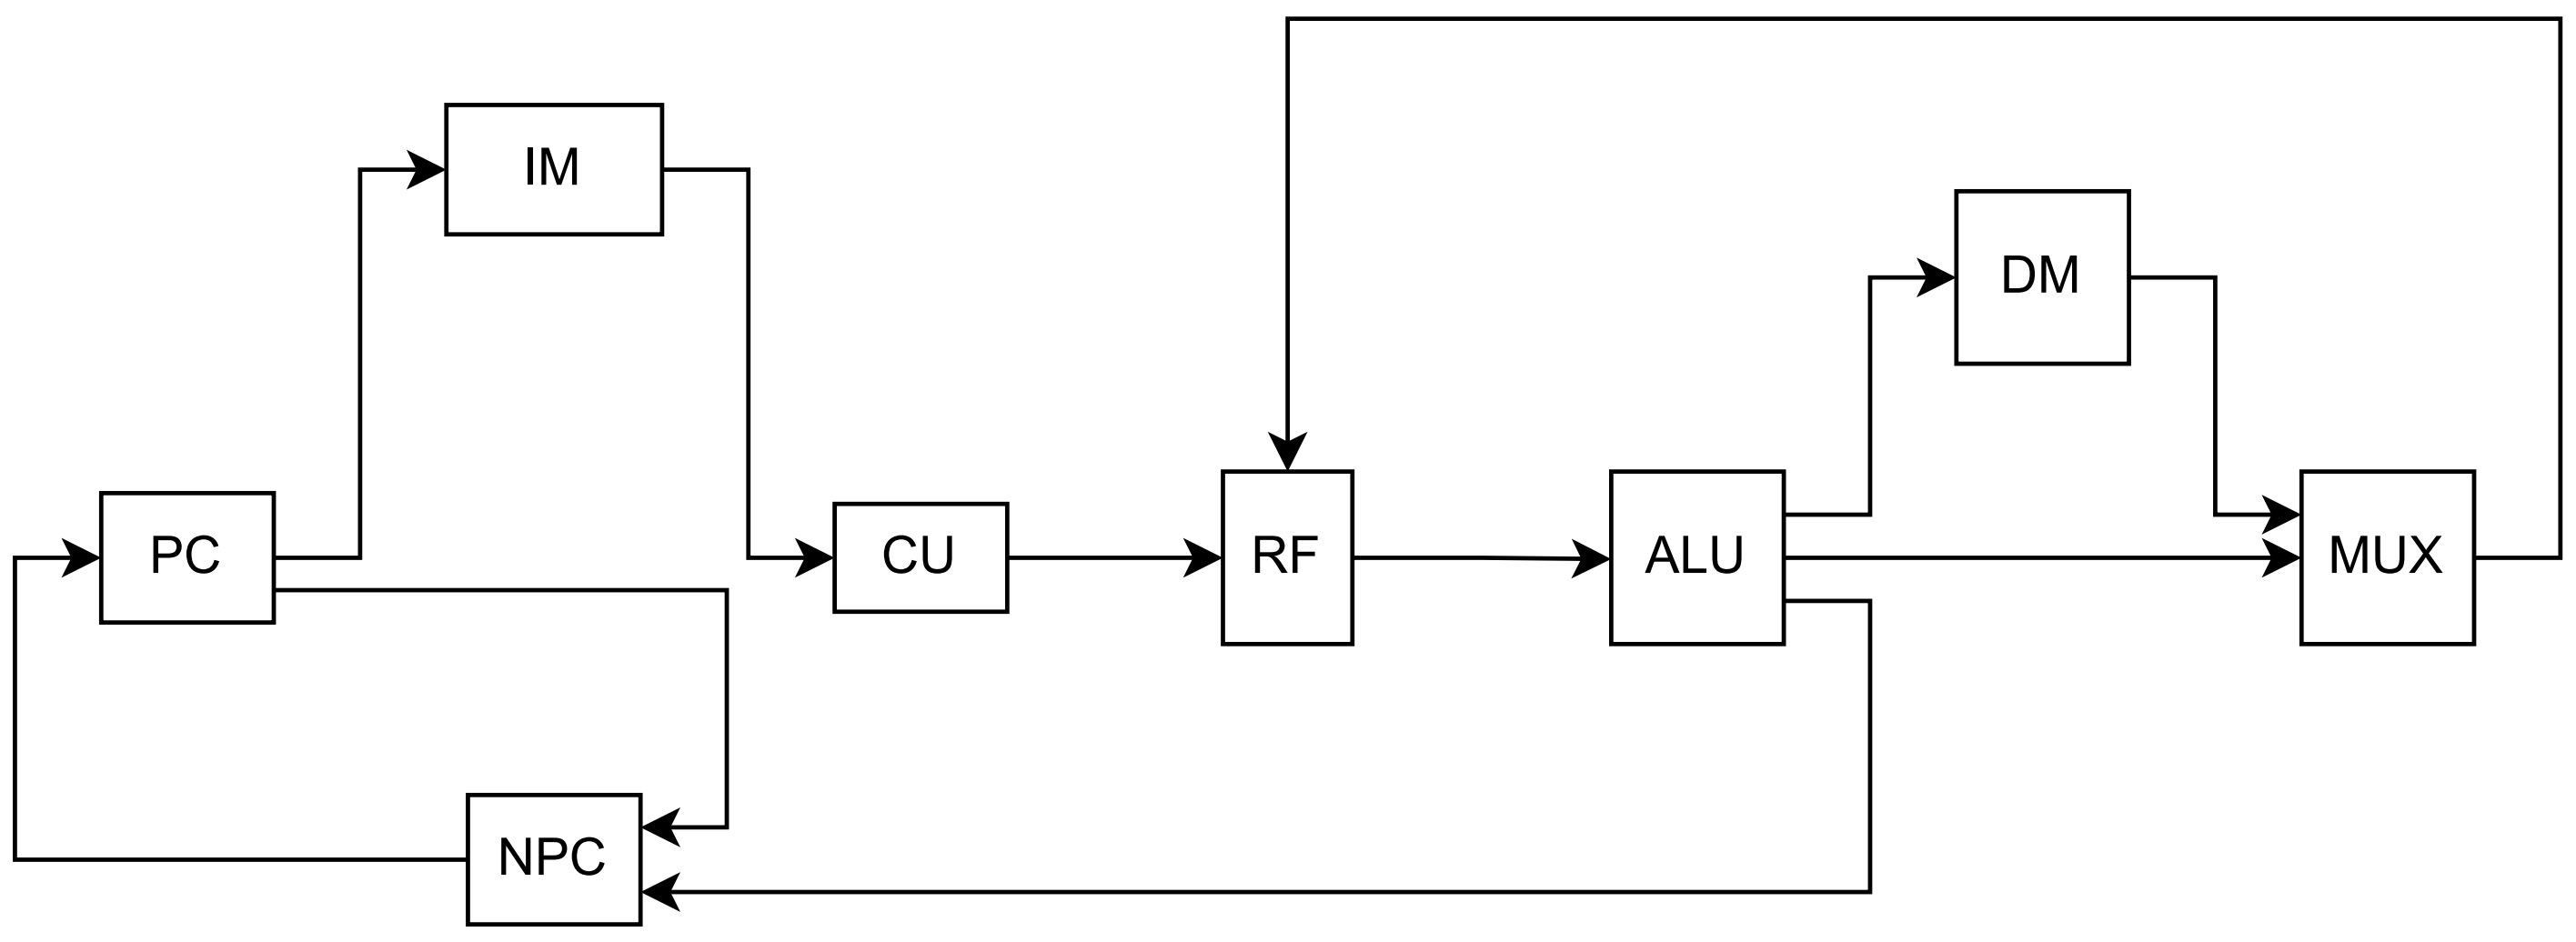
\includegraphics[width=0.75\linewidth]{assets/05/单周期处理器.png}
  \caption{单周期处理器}
  \label{fig:single-cycle-processer}
\end{figure}

如图所示，单周期处理器首先根据PC从指令存储器（IM）中取指，得到指令后进入控制器单元（CU）进行译码，得到控制信号。然后，处理器根据控制信号从寄存器堆（RF）中读取操作数，并将操作数送入ALU。如果为计算指令（如add.w），直接将ALU的结果写回；如果为访存类指令，如ld.w，还会根据ALU计算得到的访存地址从数据存储器（DM）中读值，最后，通过一个多路选择器（MUX）将指令执行结果写回RF。

对于NPC的更新，除了PC+4，还可能有源于ALU的计算结果，下一周期会根据NPC的值更新PC。

\subsection{模块设计}\label{sec:05-simple-cpu-005}

\begin{enumerate}
\def\labelenumi{\arabic{enumi}.}
\tightlist
\item
  程序计数器 (PC)：程序计数器(PC)用于存储当前正在执行的指令的地址，也就是下一条指令的地址。
\end{enumerate}

引脚：

\begin{itemize}
\item
  输入：NPC
\item
  输出：指令地址
\end{itemize}

控制信号：无

\begin{enumerate}
\def\labelenumi{\arabic{enumi}.}
\setcounter{enumi}{1}
\tightlist
\item
  算术逻辑单元 (ALU)：算术逻辑单元(ALU)执行所有的算术和逻辑运算，如加法、减法、逻辑与、逻辑或等。
\end{enumerate}

引脚：

\begin{itemize}
\item
  输入：两个操作数，操作数来源于寄存器文件或立即数。
\item
  输出：运算结果。
\end{itemize}

控制信号：

\begin{itemize}
\item
  ALUOp：指定 ALU 执行的具体操作（例如加法、减法、逻辑运算等）
\item
  ALUSrc：指定 ALU 的一个操作数来源（通常是寄存器文件或者立即数）
\end{itemize}

\begin{enumerate}
\def\labelenumi{\arabic{enumi}.}
\setcounter{enumi}{2}
\tightlist
\item
  数据存储器 (DM)：数据存储器用于存储数据，包括指令执行过程中需要读取或写入的数据。
\end{enumerate}

引脚：

\begin{itemize}
\item
  输入：地址、写入数据。
\item
  输出：从指定地址读取的数据。
\end{itemize}

控制信号：

\begin{itemize}
\item
  MemEn：存储器写使能。
\item
  MemAddr：指定要读取或写入的存储器地址。
\end{itemize}

对于add.w指令，可以设置ALUOp=ADD（对应一个枚举变量），ALUSrc=REG（代表操作数源于寄存器），ALU输入是两个寄存器的值，输出两个寄存器值的和。

对于ld.w指令，可以设置MemEn=0，MemAddr=ALURes(ALU的输出结果)，ALUSrc=IMM(代表操作数源于立即数)，ALUOp=ADD，RegEn(寄存器写使能)，ALU输入时一个寄存器的值和一个立即数，输出是两者之和。

对于st.w指令，可以设置MemEn=1，MemAddr=ALURes，ALUSrc=IMM，ALUOp=ADD，RegEn=0，ALU输入时一个寄存器的值和一个立即数，输出是两者之和。

对于beq指令，可以设置ALUOp=SUB，NPCSrc=Branch(NPC的多路选择控制信号)。

\subsection{指令实现}\label{sec:05-simple-cpu-006}

分类介绍如何给CPU添加指令，说明如何针对不同类型指令添加控制信号、书写控制模块、修改整体设计图。

假设我们已经添加了add.w、ld.w、st.w指令，下面我们将要在现有基础上添加sll.w、ld.b、bl指令。

\begin{itemize}
\tightlist
\item
  sll.w
\end{itemize}

sll.w的数据通路与add.w类似，差别仅在于ALUOp的选择。添加译码信号后，我们将控制信号中的ALUOp选择为SLL，然后在ALU中添加对应的操作，将通用寄存器rj中的数据逻辑左移，移位结果写入通用寄存器rd中。

\begin{itemize}
\tightlist
\item
  ld.b
\end{itemize}

ld.b指令的数据通路与ld.w类似，差别仅在于ld.b是从数据存储器中取回一个字节的数据符号拓展后写入通用寄存器rd，ld.w是从内存取回一个字的数据写入通用寄存器rd。因此，我们将数据从数据存储器中取出后，可以在DM后面添加一个数据后处理器模块，从一个字的数据中截取对应字节，并最终写入RF。

\begin{itemize}
\tightlist
\item
  bl
\end{itemize}

bl指令的一种简单复用现有数据通路的方式是，ALU提供给NPC的反馈信号无条件置高，然后ALU输出PC+4，并最终写回1号通用寄存器r1中。

\section{流水线CPU设计}\label{sec:05-simple-cpu-007}

本节所实现的是不考虑相关冲突的流水线CPU设计，冲突的处理详见后文。

\subsection{概念介绍}\label{sec:05-simple-cpu-008}

流水线CPU是一种通过将指令的执行过程划分为多个阶段来实现并行处理的处理器架构，这种设计有助于提高处理器的吞吐量，从而提高整体性能。下面将详细阐述流水线CPU的划分方式、各个阶段的主要功能、执行特征、以及数据通路和控制部件的概念和作用。

流水线CPU将指令执行过程分为以下五个主要阶段：

\begin{enumerate}
\def\labelenumi{\arabic{enumi}.}
\tightlist
\item
  取指阶段（IF, Instruction Fetch）：负责从内存中读取指令并将其加载到指令寄存器中。
\end{enumerate}

程序计数器（PC）提供指令的地址，然后将指令送入指令缓存，在这一阶段，处理器可能会更新程序计数器以指向下一条指令。

\begin{enumerate}
\def\labelenumi{\arabic{enumi}.}
\setcounter{enumi}{1}
\tightlist
\item
  译码阶段（ID, Instruction Decode）：负责解析指令的操作码和操作数，确定要执行的操作以及需要的寄存器。
\end{enumerate}

从寄存器堆中读取源操作数，将指令的操作码和操作数发送到执行单元准备执行。

\begin{enumerate}
\def\labelenumi{\arabic{enumi}.}
\setcounter{enumi}{2}
\tightlist
\item
  执行阶段（EX, Execution）：负责执行算术或逻辑操作，或者计算内存地址。
\end{enumerate}

执行单元（ALU、乘法器、除法器等）根据译码阶段提供的操作数和指令类型执行操作。对于内存访问指令，此阶段还计算数据的存储地址。

\begin{enumerate}
\def\labelenumi{\arabic{enumi}.}
\setcounter{enumi}{3}
\tightlist
\item
  访存阶段（MEM, Memory Access）：负责访问数据存储器（内存）以读取或写入数据。
\end{enumerate}

如果指令涉及内存操作，这一阶段将数据从内存中读取或将数据写入内存。这一阶段通常涉及数据缓存（Data Cache）的读写操作。

\begin{enumerate}
\def\labelenumi{\arabic{enumi}.}
\setcounter{enumi}{4}
\tightlist
\item
  写回阶段（WB, Write Back）：负责将计算结果写回寄存器堆。
\end{enumerate}

将执行阶段或访存阶段得到的结果写回寄存器堆中的目标寄存器，以便后续指令使用。

流水线各阶段之间通过触发器（Pipeline Registers）实现隔离和同步。这些触发器存储每个阶段的中间数据，使得每个阶段的输出可以在下一阶段使用。例如，从取指阶段到译码阶段的数据通过IF/ID触发器传递，从译码阶段到执行阶段的数据通过ID/EX触发器传递，依此类推。

在现代CPU中，为了提高数据访问的速度，通常会引入同步RAM（Synchronous RAM）。同步RAM在时钟信号的控制下进行数据存取，保证了数据的稳定性和一致性。它能与CPU的流水线操作紧密配合，以实现高效的数据存取和处理。

而在流水线处理器中，数据通路与控制部件的概念与单周期处理器类似。

\subsection{指令介绍}\label{sec:05-simple-cpu-009}

该节介绍LA32R指令中计算指令、分支跳转指令以及访存指令在流水线CPU中的处理流程。

\begin{enumerate}
\def\labelenumi{\arabic{enumi}.}
\tightlist
\item
  计算指令
\end{enumerate}

示例：add.w R1, R2, R3 （将寄存器R2和R3的值相加，并将结果存储到R1中）

\begin{itemize}
\item
  取指阶段：从指令缓存（I-cache）中获取计算指令，并将其送入指令寄存器；更新程序计数器（PC），指向下一条指令。
\item
  译码阶段：解析指令的操作码和操作数；从寄存器堆中读取源寄存器（R2、R3）的值；根据指令类型设置控制信号，指示ALU进行加法操作。
\item
  执行阶段：ALU执行加法操作，将R2和R3的值相加；计算结果准备好用于下一阶段的写回。
\item
  访存阶段：对于纯计算指令，此阶段不涉及内存访问，因此此阶段通常是空闲的。
\item
  写回阶段：将ALU的计算结果写回目标寄存器（R1）。
\end{itemize}

\begin{enumerate}
\def\labelenumi{\arabic{enumi}.}
\setcounter{enumi}{1}
\tightlist
\item
  分支跳转指令
\end{enumerate}

示例：beq R1, R2, LABEL （如果寄存器R1和R2的值相等，则跳转到指定标签的位置）

\begin{itemize}
\item
  取指阶段：从指令缓存中获取分支指令；更新程序计数器（PC），通常指向下一条指令的位置。
\item
  译码阶段：解析分支指令的操作码和目标地址；确定分支条件是否满足（例如，R1是否等于R2）；预测是否发生分支（分支预测机制）。
\item
  执行阶段：计算分支条件（比较R1和R2的值）；如果分支条件满足，计算分支目标地址。
\item
  访存阶段：对于分支指令，此阶段通常不涉及内存操作，除非分支指令本身涉及数据加载。
\item
  写回阶段：分支指令通常不涉及写回阶段，除非是某些特定的分支操作。
\end{itemize}

分支跳转指令可能引发流水线停顿（Pipeline Stalls），因为流水线必须根据分支结果决定是否继续执行下一条指令。

\begin{enumerate}
\def\labelenumi{\arabic{enumi}.}
\setcounter{enumi}{2}
\tightlist
\item
  访存指令
\end{enumerate}

示例：ld.w R1, 0(R2) （从内存地址R2 + 0中加载数据到寄存器R1中）

\begin{itemize}
\item
  取指阶段：从指令缓存中获取访存指令；更新程序计数器（PC），指向下一条指令。
\item
  译码阶段：解析访存指令的操作码和目标寄存器；从寄存器堆中读取源寄存器（R2）的值，计算内存地址；设置控制信号以进行内存访问。
\item
  执行阶段：计算内存地址（R2 + 0）；准备内存访问操作。
\item
  访存阶段：执行内存访问操作，从计算出的内存地址中读取数据（对于加载指令）或将数据写入内存（对于存储指令）。
\item
  写回阶段：将从内存读取的数据写回寄存器（对于加载指令）。
\end{itemize}

对于存储指令（如st.w，将数据写入内存），访存阶段将数据写入内存而不是寄存器。

\subsection{数据通路}\label{sec:05-simple-cpu-010}

在将单周期CPU的数据通路调整为适用于流水线CPU的规范时，需要对数据通路进行更新，以支持流水线阶段的操作。特别地，对于转移指令，需要对程序计数器（PC）的更新机制进行调整。

\begin{itemize}
\item
  添加分支控制单元：引入一个分支控制单元来决定是否发生跳转。该单元根据分支指令的条件和目标地址生成分支控制信号。
\item
  计算分支目标地址：在执行阶段（EX），计算分支目标地址。这个地址通常由指令的偏移量和当前PC值计算得到。
\item
  引入多路选择器：在PC更新路径上添加多路选择器。这个多路选择器用于选择下一条指令的地址。该多路选择器有两个输入：一个是PC的默认递增值（即PC + 4），另一个是分支目标地址。
\item
  控制信号：将分支控制信号连接到多路选择器的控制输入端。根据分支条件是否满足，选择分支目标地址或PC递增值作为下一条指令的地址。
\item
  更新PC：确保PC寄存器的更新通过多路选择器的输出进行。这使得在分支跳转时，PC可以正确地更新到新的指令地址。
\end{itemize}

\subsection{控制信号的设计}\label{sec:05-simple-cpu-011}

在单周期CPU中，整个指令执行过程都在一个时钟周期内完成，控制部件主要负责生成适当的控制信号来指导指令的执行。而在流水线处理器中，指令的执行被分为多个阶段（例如取指阶段、译码阶段、执行阶段、访存阶段和写回阶段），每个阶段都需要控制信号来确保正确的操作顺序和数据流动。

其中，``ready\_go''信号（有时也被称为``ready''信号或``stall''信号）用于协调流水线各阶段之间的操作，确保数据的正确流动和防止数据冒险。这个信号通常指示某一阶段是否准备好接受新的指令或数据，或者是否需要等待。接下来我们来看``ready\_go''信号在不同流水线阶段中的取值及其含义。

\begin{enumerate}
\def\labelenumi{\arabic{enumi}.}
\tightlist
\item
  取指阶段
\end{enumerate}

\begin{itemize}
\tightlist
\item
  ready\_go取值
\end{itemize}

1：表示取指阶段可以从指令缓存中读取新指令。

0：表示取指阶段需要等待，可能是因为前一个阶段的数据还没有准备好，或者因为存在流水线停顿（stall）或数据冒险。

当``ready\_go''信号为1时，取指阶段可以继续进行，从内存或指令缓存中读取下一条指令。如果为0，则取指阶段需要等待，可能需要停顿直到所有前面的流水线阶段都准备好或满足一定的条件。

\begin{enumerate}
\def\labelenumi{\arabic{enumi}.}
\setcounter{enumi}{1}
\tightlist
\item
  译码阶段
\end{enumerate}

1：表示译码阶段可以解码当前指令并生成适当的控制信号和寄存器读取信号。

0：表示译码阶段需要等待，可能是因为前面的取指阶段没有正确读取指令，或者因为需要等待数据或控制信号的准备。

当``ready\_go''信号为1时，译码阶段可以处理当前指令并将其传递给下一个阶段。如果为0，则表示译码阶段必须等待，可能是由于数据依赖或控制信号尚未准备好。

\begin{enumerate}
\def\labelenumi{\arabic{enumi}.}
\setcounter{enumi}{2}
\tightlist
\item
  执行阶段
\end{enumerate}

1：表示执行阶段可以进行算术逻辑运算或地址计算。

0：表示执行阶段需要等待，可能是因为前面的译码阶段未能完成指令解码，或者执行阶段依赖的数据尚未准备好。

当``ready\_go''信号为1时，执行阶段可以进行指令的实际运算。如果为0，则执行阶段必须等待，通常是由于数据冒险、依赖关系未满足或流水线停顿的原因。

\begin{enumerate}
\def\labelenumi{\arabic{enumi}.}
\setcounter{enumi}{3}
\tightlist
\item
  访存阶段
\end{enumerate}

1：表示访存阶段可以从数据缓存中读取或写入数据。

0：表示访存阶段需要等待，可能是因为前面的执行阶段未完成，或者访存操作需要等待数据缓存的响应。

当``ready\_go''信号为1时，访存阶段可以进行内存读写操作。如果为0，则访存阶段需要等待，这可能是由于内存访问的延迟或缓存未准备好。

\begin{enumerate}
\def\labelenumi{\arabic{enumi}.}
\setcounter{enumi}{4}
\tightlist
\item
  写回阶段
\end{enumerate}

1：表示写回阶段可以将计算结果写回到寄存器中。

0：表示写回阶段需要等待，可能是因为前面的访存阶段未能完成，或者写回阶段需要等待数据的准备。

当``ready\_go''信号为1时，写回阶段可以将结果写入寄存器文件。如果为0，则表示写回阶段需要等待，通常是由于数据冒险或访存阶段的延迟。

\section{将CPU核集成到SoC环境中}\label{sec:05-simple-cpu-012}

在System on Chip（SoC）设计中，内存控制器、串口控制器、Flash控制器和网络控制器是核心组件，各自承担不同的功能，并协作以实现系统的整体运作。

\begin{itemize}
\item
  内存控制器：管理SoC中的内存访问，包括RAM和其他类型的内存。它协调数据在处理器和内存之间的读写操作。
\item
  串口控制器：处理串行通信，包括数据的发送和接收。常用于连接外部设备如传感器、调试接口或其他微控制器。
\item
  Flash控制器：管理闪存的读写操作，通常用于存储系统固件、启动代码或用户数据。它保证数据的长期存储和可靠性。
\item
  网络控制器：处理网络接口的通信，如Ethernet，负责数据的接收和发送以实现网络连接。
\end{itemize}

而OpenMegaSoC 提供了 SPI、SDIO、I2S、VGA、Ethernet、UART、CDBUS、I2C 等硬件外设支持。其通过AXI4和AXI4 Lite进行片内互联，地址空间如下：

\begin{enumerate}
\def\labelenumi{\arabic{enumi}.}
\tightlist
\item
  AXI4 外设地址映射
\end{enumerate}

\begin{longtable}[]{@{}
  >{\raggedright\arraybackslash}p{(\linewidth - 4\tabcolsep) * \real{0.6022}}
  >{\raggedright\arraybackslash}p{(\linewidth - 4\tabcolsep) * \real{0.2688}}
  >{\raggedright\arraybackslash}p{(\linewidth - 4\tabcolsep) * \real{0.1290}}@{}}
\toprule\noalign{}
\begin{minipage}[b]{\linewidth}\raggedright
Address Range
\end{minipage} & \begin{minipage}[b]{\linewidth}\raggedright
Device
\end{minipage} & \begin{minipage}[b]{\linewidth}\raggedright
Select Value
\end{minipage} \\
\midrule\noalign{}
\endhead
\bottomrule\noalign{}
\endlastfoot
\texttt{0x00000000\ -\ 0x0FFFFFFF} & Memory Controller & 0 \\
\texttt{0x1C000000\ -\ 0x1C0FFFFF}\newline{}\texttt{0x1D000000\ -\ 0x1D00FFFF} & SPI Device & 1 \\
\texttt{0x1D010000\ -\ 0x1D0FFFFF} & AXI-Lite Device & 2 \\
\texttt{0x1D100000\ -\ 0x1D1FFFFF} & USB Controller & 3 \\
Other Addresses & AXI-Lite Device (Default) & 2 \\
\end{longtable}

\begin{enumerate}
\def\labelenumi{\arabic{enumi}.}
\setcounter{enumi}{1}
\tightlist
\item
  AXI4 Lite 外设地址映射
\end{enumerate}

\begin{longtable}[]{@{}
  >{\raggedright\arraybackslash}p{(\linewidth - 4\tabcolsep) * \real{0.3731}}
  >{\raggedright\arraybackslash}p{(\linewidth - 4\tabcolsep) * \real{0.4478}}
  >{\raggedright\arraybackslash}p{(\linewidth - 4\tabcolsep) * \real{0.1791}}@{}}
\toprule\noalign{}
\begin{minipage}[b]{\linewidth}\raggedright
Address Range
\end{minipage} & \begin{minipage}[b]{\linewidth}\raggedright
Device
\end{minipage} & \begin{minipage}[b]{\linewidth}\raggedright
Select Value
\end{minipage} \\
\midrule\noalign{}
\endhead
\bottomrule\noalign{}
\endlastfoot
\texttt{0x1D010000\ -\ 0x1D03FFFF} & APB Devices (UART, I2C, CDBUS) & 1 \\
\texttt{0x1D040000\ -\ 0x1D04FFFF} & Configuration Registers & 2 \\
\texttt{0x1D050000\ -\ 0x1D05FFFF} & Ethernet Controller & 3 \\
\texttt{0x1D060000\ -\ 0x1D06FFFF} & Interrupt Controller & 4 \\
\texttt{0x1D070000\ -\ 0x1D07FFFF} & SD Controller & 5 \\
\texttt{0x1D0A0000\ -\ 0x1D0AFFFF} & JPEG Controller & 6 \\
\texttt{0x1D0B0000\ -\ 0x1D0BFFFF} & I2S Controller-0（DMA） & 7 \\
\texttt{0x1D0C0000\ -\ 0x1D0CFFFF} & I2S Controller-1（GEN） & 8 \\
\texttt{0x1D0D0000\ -\ 0x1D0DFFFF} & VGA Controller & 9 \\
Other Addresses & SRAM Controller (Default) & 0 \\
\end{longtable}

而为了接入OpenMegaSoC，你需要使得自己的CPU对外保持AXI4接口，接口具体定义如下：

% 代码语言：BookVerilog
\begin{CodeBlock}[language=BookVerilog]
module mycpu_mega_top(
  input         clock,
  input         reset,
  input         awready,
  output        awvalid,
  output [31:0] awaddr,
  output [2:0]  awprot,
  output        awid,
  output        awuser,
  output [7:0]  awlen,
  output [2:0]  awsize,
  output [1:0]  awburst,
  output        awlock,
  output [3:0]  awcache,
  output [3:0]  awqos,
  input         wready,
  output        wvalid,
  output [31:0] wdata,
  output [3:0]  wstrb,
  output        wlast,
  output        bready,
  input         bvalid,
  input  [1:0]  bresp,
  input         bid,
  input         buser,
  input         arready,
  output        arvalid,
  output [31:0] araddr,
  output [2:0]  arprot,
  output        arid,
  output        aruser,
  output [7:0]  arlen,
  output [2:0]  arsize,
  output [1:0]  arburst,
  output        arlock,
  output [3:0]  arcache,
  output [3:0]  arqos,
  output        rready,
  input         rvalid,
  input  [1:0]  rresp,
  input  [31:0] rdata,
  input         rlast,
  input         rid,
  input         ruser,
  input  [7:0]  ext_int,
  output        global_reset
);
\end{CodeBlock}

\section{SoC环境下的CPU功能仿真与调试}\label{sec:05-simple-cpu-013}

为了简化仿真环境下的调试难度，eula-env中使用的仿真SoC（EulaSoC）仅包含CPU、RAM、Confreg三个设备，且片内通过AXI4总线进行互联。具体而言，CPU对外外一束AXI4总线接口，通过AXI4 Demux分为三束。对应地址空间为\texttt{0xbfaf0000\textasciitilde{}0xbfb00000}、\texttt{0x1faf0000\textasciitilde{}1fb00000}以及\texttt{0x0\textasciitilde{}0x100000000}中的其他地址空间。其中，前两束AXI4总线接口会再通过AXI4 Mux合并为一束，连接Confreg，另外一束AXI4总线接口会连接RAM。

EulaSoC中CPU的对外接口与OpenMegaSoC中CPU的对外接口保持一致，因此可延续上述接入方式。

\section{处理流水线冲突}\label{sec:05-simple-cpu-014}

\subsection{冲突类型介绍}\label{sec:05-simple-cpu-015}

在处理器中，可能存在三种冲突：

\begin{enumerate}
\def\labelenumi{\arabic{enumi}.}
\item
  资源冲突：发生在多个指令需要同一硬件资源时，例如两个指令同时访问寄存器或ALU（算术逻辑单元）。
\item
  数据冲突：发生在一条指令依赖于另一条指令的结果时，例如指令A的结果被指令B使用，但指令A还未完成。
\item
  控制冲突：发生在指令流的顺序由于分支指令而改变时，例如条件跳转指令使得处理器无法确定下一条执行指令的地址。
\end{enumerate}

\subsection{通过阻塞技术解决冲突}\label{sec:05-simple-cpu-016}

在现代处理器中，为了提高性能和避免数据冲突，处理器设计者采用了多种技术，包括阻塞技术。下面介绍了如何通过阻塞解决四种主要的数据冲突：写后写（WAW）、写后读（WAR）、读后写（RAW）、读后读（RAR）。

\begin{enumerate}
\def\labelenumi{\arabic{enumi}.}
\tightlist
\item
  写后写（WAW, Write After Write）：WAW数据冲突发生在两条指令都试图向同一个寄存器写入数据时。如果指令B试图在指令A完成写操作之前写入同一个寄存器，可能会导致数据的不确定性。
\end{enumerate}

阻塞技术可以通过在指令B写入前插入``气泡''或暂停指令执行来解决此问题。具体做法如下：

\begin{itemize}
\item
  检测冲突： 确定是否有两条指令要写入同一寄存器。
\item
  插入气泡： 在指令B的执行前插入气泡，等待指令A完成其写操作。
\end{itemize}

\begin{enumerate}
\def\labelenumi{\arabic{enumi}.}
\setcounter{enumi}{1}
\tightlist
\item
  写后读（WAR, Write After Read）：WAR数据冲突发生在一条指令试图读取某寄存器的值，而另一条指令随后写入该寄存器。如果写操作在读操作之前完成，可能导致读取到过时的数据。
\end{enumerate}

阻塞技术通过插入气泡来解决WAR冲突，确保读取操作在写入操作之前完成。具体方法包括：

\begin{itemize}
\item
  检测冲突： 确定是否有一条指令正在读取某个寄存器，同时另一条指令计划写入该寄存器。
\item
  插入气泡： 将写操作推迟，直到读取操作完成，确保数据一致性。
\end{itemize}

\begin{enumerate}
\def\labelenumi{\arabic{enumi}.}
\setcounter{enumi}{2}
\tightlist
\item
  读后写（RAW, Read After Write）：RAW数据冲突发生在一条指令试图读取一个寄存器的值，而另一条指令尚未完成对该寄存器的写入。如果读取操作在写入操作之前执行，会读取到过时的或不完整的数据。
\end{enumerate}

阻塞技术可以通过在读取操作前插入气泡来解决RAW冲突。具体步骤包括：

\begin{itemize}
\item
  检测冲突： 识别是否有一条指令需要读取一个寄存器，而另一条指令尚未完成对该寄存器的写入。
\item
  插入气泡： 暂停读取操作，直到写操作完成，确保读取到最新的值。
\end{itemize}

\begin{enumerate}
\def\labelenumi{\arabic{enumi}.}
\setcounter{enumi}{3}
\tightlist
\item
  读后读（RAR, Read After Read）：RAR数据冲突发生在两条指令都试图读取同一个寄存器。通常，RAR冲突不会引起问题，因为读取操作不改变寄存器的值，因此这种冲突比较少见。
\end{enumerate}

通常情况下，不需要特别的阻塞措施来解决RAR冲突，因为读取操作不会互相干扰。但在某些高性能处理器中，可能会通过预测和调度技术优化执行顺序。

\subsection{通过前递技术解决冲突}\label{sec:05-simple-cpu-017}

为了减少阻塞并提高处理器的执行效率，可以引入数据前递（data forwarding）通路。数据前递是一种技术，通过直接将指令的结果传递给依赖于它的后续指令，避免了不必要的等待和气泡插入。具体做法如下：

\begin{enumerate}
\def\labelenumi{\arabic{enumi}.}
\tightlist
\item
  检测数据依赖
\end{enumerate}

处理器需要识别哪些指令对前一指令的结果有数据依赖。这包括检测RAW（读后写）和WAW（写后写）冲突。处理器通过内置的数据冒险检测单元来完成这项任务。

\begin{enumerate}
\def\labelenumi{\arabic{enumi}.}
\setcounter{enumi}{1}
\tightlist
\item
  实现数据前递通路
\end{enumerate}

在流水线阶段添加前递路径：在流水线的各个阶段（如执行阶段、写回阶段），添加逻辑电路用于将指令的结果直接传递给需要这些结果的指令。对于复杂的处理器设计，可能需要多个前递通路来支持不同流水线阶段之间的数据传递。例如，从执行阶段到执行阶段，或者从写回阶段到执行阶段。

\begin{enumerate}
\def\labelenumi{\arabic{enumi}.}
\setcounter{enumi}{2}
\tightlist
\item
  调整控制逻辑
\end{enumerate}

更新控制单元：控制单元需要更新以支持数据前递，确保在依赖数据的指令中正确配置前递通路。管理数据转发：设计控制逻辑来处理转发数据的选择和路由，确保数据在正确的时间被转发到正确的指令。

\begin{enumerate}
\def\labelenumi{\arabic{enumi}.}
\setcounter{enumi}{3}
\tightlist
\item
  处理数据前递的限制
\end{enumerate}

解决数据前递延迟：确保数据前递通路的延迟最小化，以减少因转发延迟引起的性能瓶颈。管理资源竞争：处理器需要管理多个指令同时请求前递数据的情况，确保资源合理分配。

假设指令A在ALU中执行并写入寄存器R1，而指令B需要读取寄存器R1的值。如果没有数据前递，指令B必须等待指令A完成写操作。但是，通过数据前递，指令A执行的结果可以直接传递给指令B，避免了额外的等待时间，从而减少了阻塞。

% !TeX root = ../main.tex
% 原始章节：06-more-inst.Rmd

\chapter{支持更多指令设计}\label{chap:06-more-instructions}

在处理器设计中，添加新指令是一项复杂的任务，要求仔细规划和系统性的调整，下面将以EuLA处理器为例，详细介绍如何在处理器中添加指令。

\section{在流水线中添加简单运算类指令}\label{sec:06-more-instructions-001}

算术运算类指令：add.w、addi.w、pcaddu12i

比较运算类指令：slt、slti

逻辑运算类指令：and、or、nor、xor、andi、ori、xori

移位运算类指令：sll.w、sra.w、srli.w

\subsection{算术运算类指令}\label{sec:06-more-instructions-002}

以add.w和addi.w指令为例。

\begin{enumerate}
\def\labelenumi{\arabic{enumi}.}
\tightlist
\item
  添加译码信号
\end{enumerate}

% 代码语言：scala
\begin{CodeBlock}
// src/main/scala/eulacore/isa/la32r
object LA32R_ALUInstr extends HasLa32rInstrType with HasEulaCoreParameter {
  def ADDW    = BitPat("b0 0 0 0 0 0 0 0 0 0 0 1 0 0 0 0 0_?????_?????_?????")
  def ADDIW   = BitPat("b0 0 0 0 0 0 1 0 1 0_????????????_?????_?????")
  def PCADDU12I = BitPat("b0 0 0 1 1 1 0_????????????????????_?????")

  val table = Array( // (instrType, FuType, FuOpType, isrfWen)
    ADDW        -> List(Instr3R, FuType.alu, La32rALUOpType.add, true.B),
    ADDIW       -> List(Instr2RI12, FuType.alu, La32rALUOpType.add, true.B),
    PCADDU12I   -> List(Instr1RI20, FuType.alu, La32rALUOpType.pcaddu12i, true.B),
  )
}
\end{CodeBlock}

这说明，add.w和addi.w指令需要通过ALU得到计算结果，并且ALU会进行加法操作，最终操作结果会写回寄存器。根据instrType信号，会进行操作数选择，可以参考：

% 代码语言：scala
\begin{CodeBlock}
// src/main/scala/eulacore/frontend/IDU.scala
val SrcTypeTable = List(
    Instr3R     -> (SrcType.reg, SrcType.reg),
    Instr2RI12  -> (SrcType.reg, SrcType.imm),
    Instr1RI20  -> (SrcType.imm, SrcType.imm),
  )
\end{CodeBlock}

这说明add.w指令均使用寄存器值作为操作数，而addi.w指令其中一个操作数源于寄存器。对于Instr2RI12指令，其操作数会对指令的21\textasciitilde10位进行符号拓展：

% 代码语言：scala
\begin{CodeBlock}
// src/main/scala/eulacore/frontend/IDU.scala
val imm = LookupTree(instrType, List(
    Instr2RI12    -> SignExt(instr(21, 10), XLEN),
    Instr1RI20    -> SignExt(instr(24, 5), XLEN),
  ))
\end{CodeBlock}

\begin{enumerate}
\def\labelenumi{\arabic{enumi}.}
\setcounter{enumi}{1}
\tightlist
\item
  修改ALU
\end{enumerate}

% 代码语言：scala
\begin{CodeBlock}
// src/main/scala/eulacore/backend/fu/ALU.scala
class La32rALU(hasBru : Boolean = false) extends AbstractALU {

  val rj = src1
  val rk = src2
  val imm = io.offset

  val adderRes = (src1 +& (src2 ^ Fill(XLEN, isAdderSub))) + isAdderSub

  val aluRes = LookupTreeDefault(func, adderRes, List(
    La32rALUOpType.add   -> adderRes,
    La32rALUOpType.pcaddu12i -> (src1 + Cat(src2(19, 0), 0.U(12.W))),
  ))
}
\end{CodeBlock}

\subsection{比较运算类指令}\label{sec:06-more-instructions-003}

\begin{enumerate}
\def\labelenumi{\arabic{enumi}.}
\tightlist
\item
  添加译码信号
\end{enumerate}

% 代码语言：scala
\begin{CodeBlock}
// src/main/scala/eulacore/isa/la32r
object LA32R_ALUInstr extends HasLa32rInstrType with HasEulaCoreParameter {
  def SLT     = BitPat("b0 0 0 0 0 0 0 0 0 0 0 1 0 0 1 0 0_?????_?????_?????")
  def SLTI    = BitPat("b0 0 0 0 0 0 1 0 0 0_????????????_?????_?????")

  val table = Array( // (instrType, FuType, FuOpType, isrfWen)
    SLT         -> List(Instr3R, FuType.alu, La32rALUOpType.slt, true.B),
    SLTI        -> List(Instr2RI12, FuType.alu, La32rALUOpType.slt, true.B),
  )
}
\end{CodeBlock}

\begin{enumerate}
\def\labelenumi{\arabic{enumi}.}
\setcounter{enumi}{1}
\tightlist
\item
  修改ALU
\end{enumerate}

% 代码语言：scala
\begin{CodeBlock}
// src/main/scala/eulacore/backend/fu/ALU.scala
class La32rALU(hasBru : Boolean = false) extends AbstractALU {

  val rj = src1
  val rk = src2
  val imm = io.offset

  val aluRes = LookupTreeDefault(func, adderRes, List(
     La32rALUOpType.slt   -> (rj.asSInt() < rk.asSInt()),
  ))
}
\end{CodeBlock}

\subsection{逻辑运算类指令}\label{sec:06-more-instructions-004}

\begin{enumerate}
\def\labelenumi{\arabic{enumi}.}
\tightlist
\item
  添加译码信号
\end{enumerate}

% 代码语言：scala
\begin{CodeBlock}
// src/main/scala/eulacore/isa/la32r/LA32R.scala
object LA32R_ALUInstr extends HasLa32rInstrType with HasEulaCoreParameter {
  def NOR     = BitPat("b0 0 0 0 0 0 0 0 0 0 0 1 0 1 0 0 0_?????_?????_?????")
  def AND     = BitPat("b0 0 0 0 0 0 0 0 0 0 0 1 0 1 0 0 1_?????_?????_?????")
  def OR      = BitPat("b0 0 0 0 0 0 0 0 0 0 0 1 0 1 0 1 0_?????_?????_?????")
  def XOR     = BitPat("b0 0 0 0 0 0 0 0 0 0 0 1 0 1 0 1 1_?????_?????_?????")
  def ANDI    = BitPat("b0 0 0 0 0 0 1 1 0 1_????????????_?????_?????")
  def ORI     = BitPat("b0 0 0 0 0 0 1 1 1 0_????????????_?????_?????")
  def XORI    = BitPat("b0 0 0 0 0 0 1 1 1 1_????????????_?????_?????")

  val table = Array( // (instrType, FuType, FuOpType, isrfWen)
    NOR         -> List(Instr3R, FuType.alu, La32rALUOpType.nor, true.B),
    AND         -> List(Instr3R, FuType.alu, La32rALUOpType.and, true.B),
    OR          -> List(Instr3R, FuType.alu, La32rALUOpType.or, true.B),
    XOR         -> List(Instr3R, FuType.alu, La32rALUOpType.xor, true.B),
    ANDI        -> List(Instr2RI12ZEXT, FuType.alu, La32rALUOpType.and, true.B),
    ORI         -> List(Instr2RI12ZEXT, FuType.alu, La32rALUOpType.or, true.B),
    XORI        -> List(Instr2RI12ZEXT, FuType.alu, La32rALUOpType.xor, true.B),
  )
}
\end{CodeBlock}

% 代码语言：scala
\begin{CodeBlock}
// // src/main/scala/eulacore/frontend/IDU.scala
 val SrcTypeTable = List(
    Instr2RI12ZEXT -> (SrcType.reg, SrcType.imm),
  )
\end{CodeBlock}

% 代码语言：scala
\begin{CodeBlock}
// // src/main/scala/eulacore/frontend/IDU.scala
val imm = LookupTree(instrType, List(
    Instr2RI12ZEXT -> ZeroExt(instr(21, 10), XLEN),
  ))
\end{CodeBlock}

\begin{enumerate}
\def\labelenumi{\arabic{enumi}.}
\setcounter{enumi}{1}
\tightlist
\item
  修改ALU
\end{enumerate}

% 代码语言：scala
\begin{CodeBlock}
// src/main/scala/eulacore/backend/fu/ALU.scala
class La32rALU(hasBru : Boolean = false) extends AbstractALU {

  val rj = src1
  val rk = src2
  val imm = io.offset

  val aluRes = LookupTreeDefault(func, adderRes, List(
      La32rALUOpType.nor   -> ~orRes,
      La32rALUOpType.and   -> (rj & rk),
      La32rALUOpType.or    -> orRes,
      La32rALUOpType.xor   -> (rj ^ rk),
  ))
}
\end{CodeBlock}

\subsection{移位运算类指令}\label{sec:06-more-instructions-005}

\begin{enumerate}
\def\labelenumi{\arabic{enumi}.}
\tightlist
\item
  添加译码信号
\end{enumerate}

% 代码语言：scala
\begin{CodeBlock}
// src/main/scala/eulacore/isa/la32r/LA32R.scala
object LA32R_ALUInstr extends HasLa32rInstrType with HasEulaCoreParameter {
  def SLLW    = BitPat("b0 0 0 0 0 0 0 0 0 0 0 1 0 1 1 1 0_?????_?????_?????")
  def SRLW    = BitPat("b0 0 0 0 0 0 0 0 0 0 0 1 0 1 1 1 1_?????_?????_?????")
  def SRAW    = BitPat("b0 0 0 0 0 0 0 0 0 0 0 1 1 0 0 0 0_?????_?????_?????")
  def SLLIW   = BitPat("b0 0 0 0 0 0 0 0 0 1 0 0 0 0_001_?????_?????_?????")
  def SRLIW   = BitPat("b0 0 0 0 0 0 0 0 0 1 0 0 0 1_001_?????_?????_?????")
  def SRAIW   = BitPat("b0 0 0 0 0 0 0 0 0 1 0 0 1 0_001_?????_?????_?????")

  val table = Array( // (instrType, FuType, FuOpType, isrfWen)
    SLLW        -> List(Instr3R, FuType.alu, La32rALUOpType.sll, true.B),
    SRLW        -> List(Instr3R, FuType.alu, La32rALUOpType.srl, true.B),
    SRAW        -> List(Instr3R, FuType.alu, La32rALUOpType.sra, true.B),
    SLLIW       -> List(Instr2RI5, FuType.alu, La32rALUOpType.sll, true.B),
    SRLIW       -> List(Instr2RI5, FuType.alu, La32rALUOpType.srl, true.B),
    SRAIW       -> List(Instr2RI5, FuType.alu, La32rALUOpType.sra, true.B),
  )
}
\end{CodeBlock}

% 代码语言：scala
\begin{CodeBlock}
// src/main/scala/eulacore/frontend/IDU.scala
val SrcTypeTable = List(
    Instr2RI5   -> (SrcType.reg, SrcType.imm),
)
\end{CodeBlock}

% 代码语言：scala
\begin{CodeBlock}
// src/main/scala/eulacore/frontend/IDU.scala
val imm = LookupTree(instrType, List(
    Instr2RI5     -> ZeroExt(instr(14, 10), XLEN),
))
\end{CodeBlock}

\begin{enumerate}
\def\labelenumi{\arabic{enumi}.}
\setcounter{enumi}{1}
\tightlist
\item
  修改ALU
\end{enumerate}

% 代码语言：scala
\begin{CodeBlock}
// src/main/scala/eulacore/backend/fu/ALU.scala
class La32rALU(hasBru : Boolean = false) extends AbstractALU {

  val rj = src1
  val rk = src2
  val imm = io.offset

  val aluRes = LookupTreeDefault(func, adderRes, List(
      La32rALUOpType.sll   -> sllRes,
      La32rALUOpType.srl   -> srlRes,
      La32rALUOpType.sra   -> sraRes,
  ))
}
\end{CodeBlock}

\section{在流水线中添加乘除类指令}\label{sec:06-more-instructions-006}

\begin{enumerate}
\def\labelenumi{\arabic{enumi}.}
\tightlist
\item
  添加译码信号
\end{enumerate}

% 代码语言：scala
\begin{CodeBlock}
// src/main/scala/eulacore/isa/la32r/LA32R.scala
object LA32R_MDUInstr extends HasLa32rInstrType with HasEulaCoreParameter {
 def MULW    = BitPat("b0 0 0 0 0 0 0 0 0 0 0 1 1 1 0 0 0_?????_?????_?????")
 def MULHW   = BitPat("b0 0 0 0 0 0 0 0 0 0 0 1 1 1 0 0 1_?????_?????_?????")
 def MULHWU  = BitPat("b0 0 0 0 0 0 0 0 0 0 0 1 1 1 0 1 0_?????_?????_?????")
 def DIVW    = BitPat("b0 0 0 0 0 0 0 0 0 0 1 0 0 0 0 0 0_?????_?????_?????")
 def MODW    = BitPat("b0 0 0 0 0 0 0 0 0 0 1 0 0 0 0 0 1_?????_?????_?????")
 def DIVWU   = BitPat("b0 0 0 0 0 0 0 0 0 0 1 0 0 0 0 1 0_?????_?????_?????")
 def MODWU   = BitPat("b0 0 0 0 0 0 0 0 0 0 1 0 0 0 0 1 1_?????_?????_?????")

 val table = Array( // (instrType, FuType, FuOpType, isrfWen)
   MULW      -> List(Instr3R, FuType.mdu, MDUOpType.mul, true.B),
   MULHW     -> List(Instr3R, FuType.mdu, MDUOpType.mulh, true.B),
   MULHWU    -> List(Instr3R, FuType.mdu, MDUOpType.mulhu, true.B),
   DIVW      -> List(Instr3R, FuType.mdu, MDUOpType.div, true.B),
   DIVWU     -> List(Instr3R, FuType.mdu, MDUOpType.divu, true.B),
   MODW      -> List(Instr3R, FuType.mdu, MDUOpType.rem, true.B),
   MODWU     -> List(Instr3R, FuType.mdu, MDUOpType.remu, true.B),
 )
}
\end{CodeBlock}

FuType 选择 FuType.mdu，指令在后端时会选择乘除器（MDU）作为功能单元，MDU会根据 MDUOpType 选择对应操作。

\begin{enumerate}
\def\labelenumi{\arabic{enumi}.}
\setcounter{enumi}{1}
\tightlist
\item
  添加乘除法器
\end{enumerate}

出于面积和成本的限制，乘法器可以有不同的实现方式，例如一位移位乘法器、booth两位移位乘法器、华莱士树型乘法器。高性能的乘法器可通过面积换时间，通过提高设计复杂度降低惩罚执行周期数或周期延迟，除法器同样具有多种实现方式。而由于不同算法的差异，乘除器进行乘法或除法的时间不固定，因此接入时需要与前后模块增加握手信号，以保证数据的有效传输。

乘除器的一种实现方式可参见 \url{https://github.com/BUAA-CI-LAB/eulacore/blob/main/src/main/scala/eulacore/backend/fu/MDU.scala}

添加乘除法器后，在后端进行实例化，数据通过握手信号 valid-ready 进行写入。

\section{在流水线中添加转移和访存指令}\label{sec:06-more-instructions-007}

转移指令：beq、bne、b、jirl
访存指令：ld.w、st.w

\subsection{转移指令}\label{sec:06-more-instructions-008}

\begin{enumerate}
\def\labelenumi{\arabic{enumi}.}
\tightlist
\item
  添加译码信号
\end{enumerate}

% 代码语言：scala
\begin{CodeBlock}
// src/main/scala/eulacore/isa/la32r/LA32R.scala
object LA32R_BRUInstr extends HasLa32rInstrType with HasEulaCoreParameter {
  def JIRL  = BitPat("b0 1 0 0 1 1_????????????????_?????_?????")
  def B     = BitPat("b0 1 0 1 0 0_????????????????_??????????")
  def BL    = BitPat("b0 1 0 1 0 1_????????????????_??????????")
  def BEQ   = BitPat("b0 1 0 1 1 0_????????????????_?????_?????")
  def BNE   = BitPat("b0 1 0 1 1 1_????????????????_?????_?????")
  def BLT   = BitPat("b0 1 1 0 0 0_????????????????_?????_?????")
  def BGE   = BitPat("b0 1 1 0 0 1_????????????????_?????_?????")
  def BLTU  = BitPat("b0 1 1 0 1 0_????????????????_?????_?????")
  def BGEU  = BitPat("b0 1 1 0 1 1_????????????????_?????_?????")

  val table = Array( // (instrType, FuType, FuOpType, isrfWen)
    JIRL      -> List(Instr2RI16, FuType.bru, La32rALUOpType.jirl, true.B),
    B         -> List(InstrI26, FuType.bru, La32rALUOpType.b, false.B),
    BL        -> List(InstrI26, FuType.bru, La32rALUOpType.call, true.B),
    BEQ       -> List(InstrBranch, FuType.bru, La32rALUOpType.beq, false.B),
    BNE       -> List(InstrBranch, FuType.bru, La32rALUOpType.bne, false.B),
    BLT       -> List(InstrBranch, FuType.bru, La32rALUOpType.blt, false.B),
    BGE       -> List(InstrBranch, FuType.bru, La32rALUOpType.bge, false.B),
    BLTU      -> List(InstrBranch, FuType.bru, La32rALUOpType.bltu, false.B),
    BGEU      -> List(InstrBranch, FuType.bru, La32rALUOpType.bgeu, false.B),
  )
}
\end{CodeBlock}

% 代码语言：scala
\begin{CodeBlock}
// src/main/scala/eulacore/frontend/IDU.scala
val SrcTypeTable = List(
    Instr2RI16  -> (SrcType.reg, SrcType.imm),
    InstrI26    -> (SrcType.imm, SrcType.imm),
    InstrBranch -> (SrcType.reg, SrcType.reg),
  )
\end{CodeBlock}

% 代码语言：scala
\begin{CodeBlock}
// src/main/scala/eulacore/frontend/IDU.scala
 val imm = LookupTree(instrType, List(
    Instr2RI16    -> SignExt(instr(25, 10), XLEN),
    InstrI26      -> SignExt(Cat(instr(9, 0), instr(25, 10)), XLEN),
    InstrBranch   -> SignExt(instr(25, 10), XLEN),
  ))
\end{CodeBlock}

\begin{enumerate}
\def\labelenumi{\arabic{enumi}.}
\setcounter{enumi}{1}
\tightlist
\item
  添加分支跳转单元
\end{enumerate}

分支跳转指令进入 BRU 后，会计算实际跳转地址，并跟指令 NPC 进行比对，如果比对失败，则会对指令附加分支预测失败的相关信息，指令在 ROB 退休时进行前端重定向。

在 eulacore 中，BRU 复用了 ALU，可以参考 \url{https://github.com/BUAA-CI-LAB/eulacore/blob/main/src/main/scala/eulacore/backend/fu/ALU.scala}

\subsection{访存指令}\label{sec:06-more-instructions-009}

\begin{enumerate}
\def\labelenumi{\arabic{enumi}.}
\tightlist
\item
  添加译码信号
\end{enumerate}

% 代码语言：scala
\begin{CodeBlock}
// src/main/scala/eulacore/isa/la32r/LA32R.scala
object LA32R_LSUInstr extends HasLa32rInstrType with HasEulaCoreParameter {
  def LDB   = BitPat("b0 0 1 0 1 0 0 0 0 0_????????????_?????_?????")
  def LDH   = BitPat("b0 0 1 0 1 0 0 0 0 1_????????????_?????_?????")
  def LDW   = BitPat("b0 0 1 0 1 0 0 0 1 0_????????????_?????_?????")
  def STB   = BitPat("b0 0 1 0 1 0 0 1 0 0_????????????_?????_?????")
  def STH   = BitPat("b0 0 1 0 1 0 0 1 0 1_????????????_?????_?????")
  def STW   = BitPat("b0 0 1 0 1 0 0 1 1 0_????????????_?????_?????")
  def LDBU  = BitPat("b0 0 1 0 1 0 1 0 0 0_????????????_?????_?????")
  def LDHU  = BitPat("b0 0 1 0 1 0 1 0 0 1_????????????_?????_?????")
  def LLW = BitPat("b0 0 1 0 0 0 0 0_??????????????_?????_?????")
  def SCW = BitPat("b0 0 1 0 0 0 0 1_??????????????_?????_?????")

  val table = Array( // (instrType, FuType, FuOpType, isrfWen)
    LDB       -> List(Instr2RI12, FuType.lsu, La32rLSUOpType.lb, true.B),
    LDH       -> List(Instr2RI12, FuType.lsu, La32rLSUOpType.lh, true.B),
    LDW       -> List(Instr2RI12, FuType.lsu, La32rLSUOpType.lw, true.B),
    STB       -> List(InstrStore, FuType.lsu, La32rLSUOpType.sb, false.B),
    STH       -> List(InstrStore, FuType.lsu, La32rLSUOpType.sh, false.B),
    STW       -> List(InstrStore, FuType.lsu, La32rLSUOpType.sw, false.B),
    LDBU      -> List(Instr2RI12, FuType.lsu, La32rLSUOpType.lbu, true.B),
    LDHU      -> List(Instr2RI12, FuType.lsu, La32rLSUOpType.lhu, true.B),
    LLW       -> List(Instr2R, FuType.lsu, La32rLSUOpType.llw, true.B),
    SCW       -> List(InstrStore, FuType.lsu, La32rLSUOpType.scw, true.B),
  )
}
\end{CodeBlock}

\begin{enumerate}
\def\labelenumi{\arabic{enumi}.}
\setcounter{enumi}{1}
\tightlist
\item
  添加访存单元
\end{enumerate}

出于简易考虑，eulacore 采用了非流水的访存单元，每次仅可处理一条访存请求，并通过握手信号与前后模块进行联系。具体实现可以参考 \url{https://github.com/BUAA-CI-LAB/eulacore/blob/main/src/main/scala/eulacore/backend/fu/La32rUnpipelinedLSU.scala}

为了使得访存请求处理更为高效，在更复杂的处理器架构中，还可以使用流水化的访存单元，以此提高访存指令的吞吐量。在流水化访存单元中，存在两个FIFO缓存，分别是访存请求缓存和store请求缓存。每周期至多向访存单元送入一条访存请求，请求写入reqBuf后，reqBuf头指针移动。

% !TeX root = ../main.tex
% 原始章节：07-exception.Rmd

\chapter{支持异常和中断}\label{chap:07-exceptions}

截至目前，本书中介绍的CPU设计仅处理了所有指令在没有错误的情况下，按照指令语义逐条执行的情形。给定一个程序（指令序列），计算机的执行过程是确定性的。然而，实际计算机工作过程中情况往往更加复杂。

本章将从现代计算机的并行计算和内存管理两个功能入手，讨论为什么CPU需要异常和中断机制，帮助读者理解异常和中断的功能。接下来，本章将结合LA32R架构，分析该架构中异常和中断的分类。然后，从CPU的角度详细介绍处理器对异常和中断的处理流程。最后，本章将面向CPU设计，针对具体的异常类别介绍设计要点。

\section{中断和异常机制和基本概念}\label{sec:07-exceptions-001}

\subsection{CPU的中断机制}\label{sec:07-exceptions-002}

并行计算是计算机实际使用中的一个基础内容，即使是单核CPU在操作系统的控制下也可以实现并行计算。操作系统通过分时机制，让需要并行执行的多个程序交替运行。例如，让程序A先执行若干个周期，再让程序B执行若干个周期。并行计算给程序员和用户提供了两种错觉：

\begin{enumerate}
\def\labelenumi{\arabic{enumi}.}
\item
  \textbf{程序员的错觉}：程序员只需独立编写程序A和程序B，并行计算无需修改这两个程序，只需通知操作系统即可。这就是现代并行计算给程序员的错觉，即在编程时无需考虑当前程序如何与其他程序并行执行。
\item
  \textbf{用户的错觉}：尽管只有一个CPU核心，操作系统通过将两个程序的时间片划分得足够小，用户会误以为两个程序在同时运行，这便是给用户的并行错觉。
\end{enumerate}

在本文已介绍的CPU架构中，如何为操作系统提供程序切换的支持？为了从程序A跳转到程序B，传统的方法可能需要在程序A中插入跳转或分支指令，并预先计算出程序B的入口地址，从而在执行到该指令时切换到程序B。这种方法需要修改应用程序，增加了开发的复杂性。

在实际的CPU中，实现并行计算效果依赖于CPU的\textbf{中断（Interruption）}机制。CPU中断机制是一种用于处理中断事件的硬件与软件相结合的技术。当外部设备、操作系统或程序自身发出中断请求时，CPU能够暂停当前正在执行的程序，保存其状态，并转而处理该中断请求。处理完中断后，CPU可以恢复先前程序的执行，从而保证程序执行的连续性。

操作系统利用中断机制实现并行计算。每当时间片结束或有重要事件发生时（例如，I/O完成或用户输入），操作系统会触发一个中断信号。CPU收到中断后，暂停当前程序的执行，保存其上下文信息，然后跳转到操作系统的中断处理程序。这一过程中，操作系统可以根据需要切换到另一个待执行的程序。通过这种方法，操作系统无需修改用户程序就能实现程序的快速切换，达到并行计算的效果。

\subsection{CPU的异常机制}\label{sec:07-exceptions-003}

内存管理是操作系统的重要功能之一，它确保多个程序能够在受限的物理内存中安全、高效地运行。为了让程序员能够在不考虑实际物理内存布局的情况下编写代码，操作系统引入了虚拟内存机制。虚拟内存为每个程序提供了独立的地址空间，使得程序员无需关心程序间的内存冲突问题。

在虚拟内存管理中，操作系统将物理内存划分为多个固定大小的页面，并将这些页面映射到程序的虚拟地址空间中。程序在执行时，通过CPU的内存管理单元（MMU）将虚拟地址转换为物理地址。这种地址转换使得程序可以在比实际物理内存更大的地址空间中运行，而操作系统负责管理这些映射关系。

然而，当程序访问的虚拟地址没有被映射到物理内存时，就会出现一个关键问题：CPU无法完成这次内存访问。在这种情况下，虚拟内存机制依赖于CPU提供的异常支持。当发生这种情况时，CPU会触发一个页错误异常，暂停当前程序的执行，并将控制权交给操作系统的异常处理程序。

操作系统通过异常处理程序可以加载所需的页面或处理其他内存管理问题，然后将控制权返回给CPU，继续程序的执行。通过这种方式，虚拟内存得以有效运作，而这一切都依赖于CPU的异常机制。

\textbf{异常（Exception）}是一种由程序执行过程中发生的错误或特殊事件触发的机制。当程序访问了无效的页面，或者发生了其他导致指令无法正常执行的情况时，CPU会自动暂停当前指令的执行，保存程序的状态，并跳转到异常处理程序。操作系统在异常处理程序中，可以采取多种措施来解决问题。

页错误异常指的是，当程序访问了一个未映射的虚拟地址时，CPU触发页错误异常。操作系统可以通过检查访问的地址，判断是否需要将对应的页面从磁盘加载到物理内存中，并更新页表。处理完这一异常后，操作系统可以让CPU恢复到错误发生前的状态，并重新执行引发异常的指令，从而让程序继续运行。

通过异常机制，操作系统能够灵活管理内存，提高系统的稳定性和健壮性。程序员不必在每个可能的内存访问错误上插入额外的错误检查逻辑，而是依赖于操作系统的异常处理机制，确保程序在遇到问题时能得到妥善处理。异常机制不仅使得程序更加简洁，还提高了系统资源的利用效率。

\subsection{基本概念}\label{sec:07-exceptions-004}

\textbf{异常（Exception）和中断（Interrupt）}是两类会打断CPU正常指令执行的事件。它们都使得CPU暂停当前的指令流，并转向预定义的处理程序，从而应对突发的情况。然而，二者在触发原因和处理方式上存在显著差异。

异常是由程序执行过程中发生的错误或特殊事件引发的。常见的异常包括除零错误、非法指令、页面错误（如访问未映射的虚拟地址）等。当CPU遇到这样的情况时，通常无法继续执行当前指令，必须进行特殊处理。此时，CPU会自动暂停当前程序的执行，保存当前的状态信息，然后跳转到操作系统定义的异常处理程序。异常处理程序可以修复错误、报告问题，或者在某些情况下终止问题程序。异常通常是同步事件，即它们与程序的执行紧密相关，并在指令执行时被检测到。

中断则是由外部事件或硬件设备引发的，例如键盘输入、硬盘I/O完成信号、定时器超时等。当这些设备或外部事件需要CPU立即响应时，它们会向CPU发送中断信号。收到中断信号后，CPU会暂停当前任务的执行，保存任务的状态，然后跳转到对应的中断处理程序。与异常不同，中断通常是异步事件，即它们与程序执行无关，可以在任意时间发生。中断的处理通常较为简短和快速，处理完后，CPU会恢复之前的任务继续执行。中断可以分为可屏蔽中断（maskable interrupts），如一般的外部设备中断，和不可屏蔽中断（non-maskable interrupts），如系统故障或其他紧急情况。

尽管异常和中断都涉及到CPU的状态切换与处理程序的执行，但它们的区别主要在于触发条件和性质。异常是由程序内部执行错误或特殊情况引发的同步事件，直接与当前指令流相关。而中断则是由外部硬件或其他系统事件引发的异步事件，与当前程序的指令流无关。此外，异常通常需要复杂的处理逻辑来修复程序状态或报错，而中断则通常只需处理简单的硬件请求，如读取数据或响应用户输入。

异常和中断在处理机制上具有许多相似之处。首先，二者都需要CPU跳转到指定的处理程序。其次，处理完毕后，CPU需要恢复之前的状态，继续执行被打断的程序。此外，操作系统的设计通常会统一管理异常和中断的处理机制，使用类似的框架来处理这两类事件。例如，异常和中断的处理程序都需要在系统的中断向量表或异常向量表中注册，并且都可能涉及对系统资源的调度和管理。通过统一的异常和中断处理机制，操作系统能够高效地应对各种突发事件，确保系统的稳定运行。

常见的异常事件包括：

\begin{itemize}
\tightlist
\item
  除零错误：当执行除法指令时，除数为零会导致异常，此时CPU通过异常机制进行处理。
\item
  非法指令：CPU遇到无法识别或无效的指令时触发异常。
\item
  页面错误：虚拟内存管理中，当访问一个未映射到物理内存的页面时会产生异常。
\end{itemize}

常见的中断事件包括：

\begin{itemize}
\tightlist
\item
  时钟中断：用于操作系统的调度程序切换任务。
\item
  外部中断：如键盘、鼠标或网络设备的输入信号，这些外设在工作完成或需要进行信息传递时，可通过使CPU陷入中断的方式通知CPU（还有其他的外设交互方法）。这种方式需要利用CPU的外部中断。
\item
  软件中断：软件可通过给体系结构规定的特定寄存器写入某些值的方式，使CPU陷入中断。与外部中断不同的是，这种中断时软件在运行时自行触发的。
\end{itemize}

\section{异常和中断的分类}\label{sec:07-exceptions-005}

\subsection{六类异常}\label{sec:07-exceptions-006}

在LoongArch架构中，异常可以根据其来源划分为以下六种类型，每种类型都有其独特的触发条件和处理要求：

1）\textbf{外部事件}：外部事件是指源自于CPU核心外部的模块或者通过实际的物理连线从处理器外部传入的事件，通常称为中断。中断使得CPU能够异步处理多个事件，尤其是在操作系统中，中断机制避免了轮询等待的资源浪费，特别是在处理与I/O相关的任务时显得尤为重要。中断事件的不可预测性以及无法由软件控制的特性，要求系统必须具备完善的软硬件协作机制，以确保中断的处理不会干扰程序的正常执行流程。例如，外部设备发出的I/O中断信号会打断当前执行的程序，转而执行中断服务程序（\texttt{ISR}），从而提高系统的响应速度。

2）\textbf{指令执行中的错误}：在指令执行过程中，可能会发生由于操作码或操作数不符合要求而引发的错误，例如调用不存在的指令、试图进行除以零的操作、访问不对齐的地址、在用户态下调用仅供核心态使用的指令或尝试访问非法的内存地址空间等。这些错误将导致指令无法继续执行，并且可能引发严重的系统错误。因此，系统必须具备相应的异常处理机制，以确保能够在发生这些错误时及时捕获并进行适当的处理，例如通过软件捕捉这些异常并采取相应的补救措施。

3）\textbf{数据完整性问题}：数据完整性问题通常涉及存储器数据的校验错误。例如，在存储器中使用ECC（错误检测和纠正码）等硬件校验方式时，如果发现数据在传输或存储过程中发生了校验错误，系统会引发异常。这些异常可以帮助系统识别出硬件中的潜在故障，从而采取措施，如重新读取数据或修复数据错误。对于可纠正的错误，系统可以自动修正；而对于不可纠正的错误，系统可能需要重新启动或切换到冗余系统以维持正常运行。

4）\textbf{地址转换异常}：在存储管理单元（\texttt{MMU}）尝试对内存页进行地址转换时，如果在硬件的页表或转换表中找不到相应的地址映射项，就会产生地址转换异常。这类异常通常表明程序试图访问的内存地址不存在或没有被正确映射，需要异常处理程序来解决这一问题。处理器可以通过异常处理程序将缺页错误（\texttt{Page\ Fault}）转交给操作系统，由操作系统决定是分配新的内存页，还是终止错误的进程。

5）\textbf{系统调用和陷入}：系统调用和陷入异常是由特定指令触发的，旨在生成操作系统可识别的信号，以便在受保护模式下调用核心态的相关操作。通常，这类异常用于执行需要更高权限的操作，例如文件系统访问、进程管理、硬件设备控制等。系统调用通过触发陷入异常，使得用户态程序能够安全地请求操作系统服务，而不必直接操作硬件资源，从而确保系统的安全性和稳定性。

6）\textbf{需要软件修正的运算}：在某些复杂的运算过程中，特别是涉及到浮点运算指令时，由于硬件实现的复杂性，可能无法直接处理所有情况。这时，处理器会引发异常，通知系统使用软件来完成这些复杂运算。例如，某些特殊的浮点运算或者未定义的操作会触发一个浮点异常，系统可以通过软件模拟的方式来完成这些计算，保证程序的正确性和稳定性。

\subsection{两类中断}\label{sec:07-exceptions-007}

在LoongArch架构中，中断是处理器应对外部事件的一种机制，通常通过两种主要方式传递到处理器：\textbf{中断线}和\textbf{消息中断}。

1）\textbf{中断线传递}：这是最直接的中断传递方式，通常用于中断源数量较少的系统。在这种方式中，中断源通过物理中断线直接连接到处理器的中断引脚。当处理器检测到某根中断线有信号时，处理器会优先处理该中断线所对应的中断事件，并调用相应设备的中断服务程序（\texttt{ISR}）。如果系统中有多个中断源，则可能通过中断控制器来汇总这些信号，进行中断优先级的管理和中断请求的分发。

2）\textbf{消息中断传递}：消息中断是一种更具扩展性和灵活性的方法，通过向特定的内存地址写入一个指定的数值来触发中断，而不依赖于物理中断线。这种方法不仅减少了对物理引脚的依赖，还允许系统动态地分配和管理中断源。消息中断的使用非常灵活，适用于复杂的系统设计，尤其是那些拥有大量设备和中断源的现代计算机系统。例如，在多核处理器或分布式系统中，消息中断可以用于实现高效的核间通信（\texttt{Inter-Processor\ Interrupts}，简称\texttt{IPI}），或者在虚拟化环境中，实现对虚拟机的中断传递和管理。

在LoongArch32R架构中，仅需要实现第一种中断机制。

\section{异常和中断处理流程}\label{sec:07-exceptions-008}

\subsection{异常处理流程}\label{sec:07-exceptions-009}

异常处理是系统处理异常事件的关键环节，通常包括以下五个阶段：\textbf{准备处理}、\textbf{确定异常来源}、\textbf{保存执行状态}、\textbf{处理异常}以及\textbf{恢复状态并返回}。这些阶段的核心目标是确保异常处理能够准确无误地进行，同时保持系统的整体稳定性。

1）\textbf{异常处理准备}：当异常发生时，CPU需要在进入异常处理程序之前完成一些准备工作。这包括记录异常发生时被打断的指令地址和处理状态。在LoongArch架构中，\texttt{CSR.ERA}寄存器用于保存发生异常时的指令地址，从而确保处理器能够在异常处理完成后，准确恢复到异常发生前的状态，继续执行中断的程序。此外，CPU通常会将其权限等级提升到最高特权级，并关闭中断响应。在LoongArch中，通过将\texttt{CSR.CRMD}寄存器的\texttt{PLV}域设置为0进入最高权限级别，并将\texttt{IE}域置0以屏蔽所有中断，确保异常处理过程中不被新的中断干扰。

在准备阶段，硬件还需保存当前的处理状态以供恢复。例如，LoongArch架构中，\texttt{CSR.CRMD}中的\texttt{PLV}和\texttt{IE}域的旧值会被存储到\texttt{CSR.PRMD}寄存器中，这样在异常处理结束后可以快速恢复之前的状态。同时，异常编号和其他相关信息会记录在\texttt{CSR.ESTAT}寄存器的相应域中，以供异常处理程序参考和处理。

2）\textbf{确定异常来源}：不同类型的异常需要特定的处理程序来应对。处理器通过异常编号来区分不同的异常类型，并跳转到相应的异常处理程序入口。在LoongArch架构中，异常处理程序入口地址由\texttt{CSR.EENTRY}寄存器和\texttt{CSR.ECFG}寄存器的组合来确定，每种异常类型都对应一个特定的入口地址。相比之下，在X86架构中，处理器使用中断描述符表（\texttt{IDT}）来确定异常处理程序的入口地址，每种异常类型都有其对应的中断描述符，描述符中包含了处理程序的段选择子和偏移地址。

3）\textbf{保存执行状态}：在进入异常处理程序之前，操作系统通常会将当前程序的状态保存到堆栈中。这包括通用寄存器、程序计数器（\texttt{PC}）、状态寄存器（\texttt{SR}）等关键数据的内容，以便在处理完异常后能够准确地恢复被打断的程序状态。这一步骤对于确保程序能够在异常处理完毕后继续正常执行至关重要。

4）\textbf{处理异常}：一旦异常处理程序被调用，系统会根据异常的类型执行特定的处理操作。例如，对于页面错误异常，处理程序可能需要分配新的页面并更新页表；对于系统调用异常，处理程序会根据调用的系统服务号执行相应的内核操作。在LoongArch中，异常处理程序可以通过查看\texttt{CSR.ESTAT}中的异常编号和相关信息来决定处理流程，并执行相应的指令以解决异常或完成所请求的操作。

5）\textbf{恢复执行状态并返回}：在异常处理完成后，系统需要将之前保存的执行状态恢复，并使程序继续从中断处或指定位置开始执行。具体的恢复操作包括从堆栈中取出保存的寄存器值、恢复程序计数器（\texttt{PC}）以及状态寄存器的内容。在LoongArch架构中，\texttt{CSR.ERA}寄存器的值会被恢复到\texttt{PC}中，确保程序能够从正确的位置继续执行。此外，\texttt{CSR.PRMD}寄存器中的旧权限等级和中断使能状态也会被恢复到\texttt{CSR.CRMD}中，以确保程序在处理完异常后回到正确的权限级别，并重新启用中断响应。

在一些复杂的异常处理中，异常处理程序可能需要进行额外的操作，如清理资源、记录日志或发出警告等。在此情况下，处理程序在返回之前，确保所有额外的操作都已经完成，且不会影响程序的正常运行。

恢复完成后，系统通过专门的指令返回到异常发生前的程序继续执行。例如，LoongArch使用\texttt{ERET}（Exception Return）指令来恢复异常前的状态并返回到中断的程序执行，这确保了系统在处理完异常后，能够准确无误地继续原有的程序流程。

\subsection{中断的响应}\label{sec:07-exceptions-010}

LoongArch指令系统共定义了13个中断，分别是：

\begin{enumerate}
\item 1个核间中断（\texttt{IPI}），
\item 1个定时器中断（\texttt{TI}），
\item 1个性能监测计数溢出中断（\texttt{PMI}），
\item 8个外部硬中断（\texttt{HWI0\textasciitilde{}HWI7}），
\item 2个软中断（\texttt{SWI0\textasciitilde{}SWI1}）。
\end{enumerate}


所有中断线上的中断信号均采用电平中断，并且都是高电平有效。当有中断发生时，这种高电平有效的中断方式会在输入到处理器的中断线上保持高电平状态，直到中断被处理器响应并处理为止。无论中断源来自处理器核的外部还是内部，是硬件触发还是软件置位，这些中断信号都会持续地被采样，并记录到\texttt{CSR.ESTAT}中的\texttt{IS}域对应的比特位上。

这些中断均为可屏蔽中断，除了\texttt{CSR.CRMD}中的全局中断使能位\texttt{IE}外，每个中断各自还有其局部中断使能控制位，位于\texttt{CSR.ECFG}的\texttt{LIE}域中。当\texttt{CSR.ESTAT}中的\texttt{IS}域的某位为1且对应的局部中断使能和全局中断使能均有效时，处理器将响应该中断，并进入中断处理程序的入口处开始执行。

在支持多个中断源输入的指令系统中，需要明确当多个中断同时触发时，处理器如何区别不同来源的中断优先级。

\textbf{非向量中断模式}：在非向量中断模式下不区分中断优先级。此时，如果需要对中断进行优先级处理，可以通过软件方式来实现。常见的实现方案包括：

\begin{enumerate}
\item 软件随时维护一个中断优先级（\texttt{IPL}），每个中断源都被赋予特定的优先级。
\item 在正常状态下，CPU运行在最低优先级，此时任何中断都可以触发。
\item 当CPU处于最高中断优先级时，任何中断都被禁止。
\item 当更高优先级的中断发生时，可以抢占低优先级的中断处理过程。
\end{enumerate}


\textbf{向量中断模式}：在向量中断模式下，处理器通常需要依照既定的优先级规则从多个已生效的中断源中选择一个，并跳转到其对应的处理程序入口处。完整LoongArch指令系统实现的是向量中断，采用固定优先级仲裁机制，具体规则如下：硬件中断号越大，优先级越高。也就是说，\texttt{IPI}的优先级最高，\texttt{TI}次之，依次递减，直到\texttt{SWI0}，其优先级最低。由于简化版的LA32R架构无需实现向量中断，因此LA32R的开发者也不需要处理向量中断中的优先级问题。

\section{优先级}\label{sec:07-exceptions-011}

在处理器设计中，异常和中断是两类不同的事件处理机制，它们各自承担着不同的功能。\textbf{异常}通常是由于程序执行中的错误或特定指令而触发的，例如除以零、非法指令或地址不对齐等情况。而\textbf{中断}则是由外部事件或硬件信号触发的，如定时器中断、外设中断等，用于打断当前程序的执行，以便处理紧急任务。

\subsection{异常与中断的优先级}\label{sec:07-exceptions-012}

在大多数处理器架构中，\textbf{异常}的优先级通常高于\textbf{中断}。这是因为异常通常与当前指令的执行密切相关，并且如果不立即处理，可能会导致系统的不稳定或崩溃。例如，当遇到非法指令或除零错误时，处理器必须立即响应并处理，否则程序的执行将无法继续。

另一方面，中断尽管需要及时处理，但通常它们与外部事件有关，通常可以在异常处理完成后再进行响应。这种设计确保了系统在遇到严重错误时能够优先处理这些错误，维持系统的稳定性。

\subsection{精确异常}\label{sec:07-exceptions-013}

\textbf{精确异常}是指在发生异常时，处理器能够保证异常发生前的所有指令已经正确执行，而异常发生后的指令未执行或可以撤销。这意味着，当异常处理完成后，处理器能够从异常发生的指令重新开始执行，而不会丢失或重复任何指令的执行。

精确异常的实现对于处理器的可靠性至关重要，尤其是在复杂的流水线和超标量处理器中。在这些处理器中，指令的执行顺序可能与程序的顺序不同，因此在异常发生时，确保异常精确定位和处理成为了处理器设计中的一个重要挑战。

在大多数现代处理器中，硬件支持精确异常的机制。例如，在异常发生时，处理器会记录被打断的指令地址（通常存储在如\texttt{CSR.ERA}的寄存器中），确保异常处理完成后能够正确地恢复执行。

\subsection{中断的异步响应}\label{sec:07-exceptions-014}

\textbf{中断}的一个关键特性是其\textbf{异步性}。与异常不同，中断并不与指令的执行直接相关。中断可以在任何时候发生，而不受当前正在执行的指令的限制。这种异步性使得中断成为处理外部事件的有效机制，例如定时器溢出或外设的输入信号。

当中断发生时，处理器会暂停当前的指令执行，保存上下文，然后跳转到中断处理程序。在LoongArch架构中，中断信号被不断采样并记录在\texttt{CSR.ESTAT}的\texttt{IS}域中。处理器根据中断优先级决定是否响应中断，并通过跳转到中断处理程序的入口地址来处理该中断。

在实际的CPU开发过程中，中断的异步响应特性给测试工作带来了很大的困难。由于不同微架构的处理器可能对于同时出现的中断信号有不同的响应时间，因此往往没有一个固定的正确行为可供开发人员比对。因此，开发者要么对中断进行手动测试，要么开发或使用一些测试框架。本团队的敏捷开发测试框架可缓解异步中断带来的测试困难，具体可参考另一个文档。

\subsection{中断和异常的嵌套处理}\label{sec:07-exceptions-015}

在复杂的计算系统中，处理器可能会在处理一个异常或中断时再次遇到新的异常或中断，这就是中断和异常的嵌套处理。为了处理这种情况，LoongArch架构提供了灵活的机制来管理和处理嵌套的中断和异常。

1）\textbf{优先级机制}：嵌套处理中，处理器需要通过优先级机制来决定是立即处理新的异常/中断，还是先完成当前的异常/中断处理。不同的异常和中断有不同的优先级，通常外部中断的优先级最低，而系统错误类异常的优先级最高。例如，在LoongArch中，当处理一个低优先级的中断时，如果一个更高优先级的异常发生，处理器会暂时中断当前的中断处理，转而处理高优先级的异常。处理完高优先级异常后，处理器会恢复到之前的中断处理流程。

2）\textbf{状态保存与恢复}：为了正确处理嵌套的中断和异常，处理器在每次进入新的异常或中断处理程序时，都需要保存当前的状态，并在退出时恢复之前的状态。这通常涉及堆栈的使用，将每一层嵌套的上下文信息（如寄存器内容、程序计数器等）压入堆栈，以便在处理完当前的异常/中断后能够恢复到正确的处理状态。例如，在LoongArch中，每次嵌套时，\texttt{CSR.ERA}、\texttt{CSR.CRMD}、\texttt{CSR.PRMD}等寄存器的值都会保存到堆栈中，确保嵌套处理不会丢失原有的处理状态。

3）\textbf{中断屏蔽与使能}：在处理嵌套的异常/中断时，处理器可以通过屏蔽某些中断来防止进一步的嵌套。例如，当处理高优先级的异常时，可以暂时屏蔽低优先级的中断，确保处理器不被其他不重要的中断打扰。LoongArch中的\texttt{CSR.CRMD}寄存器的\texttt{IE}位用于控制全局中断使能，通过设置或清除这个位，处理器可以有效管理在嵌套处理期间的中断行为。

4）\textbf{返回机制}：在嵌套处理完成后，处理器需要逐层恢复之前的中断或异常处理状态，并正确返回到中断或异常发生前的程序执行。在LoongArch架构中，使用\texttt{ERET}指令不仅用于简单的异常返回，还能处理嵌套的情况，通过\texttt{CSR.PRMD}和\texttt{CSR.ERA}寄存器的内容，处理器可以正确返回到之前的异常或中断处理程序中，逐层退出嵌套，直至最终返回到最初的程序执行。

在LA32R中不需要支持中断的嵌套处理机制，但对嵌套机制的了解有助于进行CPU的设计，以及对软硬件协同工作原理的理解。

\section{在CPU中增加异常与中断功能的设计要点}\label{sec:07-exceptions-016}

在CPU设计中，增加异常和中断功能是实现系统健壮性和灵活性的关键步骤。为此，开发者需要从多个方面考虑，确保这些功能能够可靠且高效地处理各种异常和中断情况。

在处理器设计中，几种常见的异常和中断需要特别关注，包括\textbf{地址错}、\textbf{整形溢出}以及\textbf{系统调用}。

\begin{itemize}
\item
  \textbf{地址错异常}通常由无效的内存访问引发，比如访问未对齐的地址或越界访问。这类异常的检测逻辑通常在地址生成单元（AGU）中实现，通过检查访问地址是否符合对齐要求，以及是否在合法的地址空间范围内。如果检测到地址错误，处理器会触发异常，并跳转到对应的异常处理程序。
\item
  \textbf{整形溢出异常}发生在算术运算结果超出数据类型的表示范围时。例如，在32位整数加法中，如果结果超出32位表示范围，处理器会产生溢出异常。为了检测这种情况，算术逻辑单元（ALU）会在执行运算后检查结果的符号位与溢出位，确认是否发生了溢出。
\item
  \textbf{系统调用}是一种特殊的异常，用于在用户态下调用操作系统内核功能。系统调用通常由专用指令（如LoongArch中的\texttt{SYSCALL}指令）触发。系统调用异常的检测逻辑相对简单，只需检测到指令后触发相应的异常处理即可。
\end{itemize}

\subsection{精确异常与中断的实现}\label{sec:07-exceptions-017}

根据上文的介绍，\textbf{精确异常}是指在异常发生时，确保被异常打断的指令及其之前的指令已经完整执行，而之后的指令未被执行。在具体进行开发实现时，开发人员需要在硬件和控制逻辑中精确跟踪指令的执行状态。当发生异常时，开发人员应让处理器保存当前指令的地址（如\texttt{CSR.ERA}寄存器），并正确地维护\texttt{CSR.CRMD}和\texttt{CSR.ESTAT}等寄存器的状态，以便异常处理程序能够准确恢复并继续执行。

\begin{itemize}
\tightlist
\item
  \textbf{\texttt{CSR.ERA}}寄存器保存异常发生时的指令地址，允许异常处理结束后恢复执行。
\item
  \textbf{\texttt{CSR.CRMD}}寄存器控制处理器的模式和全局中断使能，异常发生时会自动调整权限等级。
\item
  \textbf{\texttt{CSR.ESTAT}}寄存器记录当前异常或中断的状态，包括异常编号等关键信息。
\end{itemize}

\subsection{添加异常中断的支持}\label{sec:07-exceptions-018}

要在CPU中添加系统调用异常中断的支持，首先需要在指令解码阶段识别系统调用指令。当指令解码单元识别到\texttt{SYSCALL}指令时，它会触发异常处理流程。处理器需要跳转到系统调用异常处理程序的入口地址，并保存相关上下文信息（如\texttt{CSR.ERA}和\texttt{CSR.CRMD}）。在异常处理程序中，操作系统会根据系统调用号执行相应的内核功能，并最终通过执行异常返回指令（如LoongArch中的\texttt{ERTN}指令）恢复用户态的执行。

以\textbf{地址错异常}为例，添加支持的过程类似于系统调用异常。在地址生成单元中，检测到地址错时，处理器将生成一个地址错异常信号，并保存导致异常的虚拟地址到特定寄存器（如\texttt{CSR.BADV}）。接下来，处理器会跳转到地址错异常处理程序，该程序可以记录错误信息、通知操作系统或采取修复措施。

通过逐步实现和集成这些异常和中断的检测逻辑和处理流程，开发者可以确保处理器能够正确处理各种异常情况，提高系统的可靠性和稳定性。为了确保正确性，开发者应仔细阅读指令集手册，并充分理解处理器架构中的各类寄存器和控制状态。

% !TeX root = ../main.tex
% 原始章节：08-bus-and-soc.Rmd

\chapter{总线接口与SoC集成设计}\label{chap:08-bus-and-soc}

\section{计算机总线接口}\label{sec:08-bus-and-soc-001}

一个完整的计算机系统包含多个组成部件，这些部件通常由不同的设计人员或公司开发。为了使它们能够在一起协同工作，这些部件之间需要遵循一套共同的规则和规范，这种规范就是总线协议，总线协议是连接计算机系统中不同模块之间的桥梁。例如，计算机的主板可能由一家公司开发，而CPU由另一家公司设计。为了使这两个关键部件能够正常交互，它们之间就需要通过某种总线协议进行通信。总线协议规定了如何在连接线上传输数据，包括高电平、低电平分别代表什么含义，不同信号线之间的关系，数据传输的时序安排，以及如何进行数据校验和纠错。这些规定确保发送方能够将信息编码为适合传输的格式，通过总线传递，而接收方能够正确解读传输的信号。

总线的应用和标准化大幅简化了计算机系统的设计难度。通过引入统一的标准接口，制造商能够确保其设备可以与其他厂商的产品顺利协同工作，而无需为每个组件设计不同的连接方式。例如，某制造商生产的一块主板，只要符合相应的接口标准，就可以与任何支持该标准的CPU或其他硬件设备兼容。这种标准化不仅提升了各组件之间的兼容性，也大大优化了产品开发的流程。在工业领域，像PCI和USB这样的标准总线广泛用于各类计算机系统中。

从信号传输的方式来看，总线可分为并行总线和串行总线。并行总线通过多条传输线同时传输多个数据位，而串行总线则只通过一条传输线一次传输一位数据。并行总线的优势在于它能在相同频率下提供更大的数据传输带宽，因为多个比特能够并行传输。不过，并行传输要求所有数据位必须同步到达，这对总线的宽度、频率以及主板的设计提出了较高的要求。相比之下，串行总线采用单条传输线，每次传输一个比特，并通过编码技术将时钟信号嵌入数据中，使其能够以更高的频率进行数据传输。常见的并行总线包括类SRAM总线、AXI总线，而串行总线的代表则是USB、I2C等。

根据总线在计算机系统中的实际位置，可以将总线分为片上总线、内存总线、系统总线和设备总线。片上总线主要用于连接芯片内部的各个功能模块。在芯片设计过程中，通常会将其分为多个模块，这些模块间的数据交换依赖片上总线。例如，高性能的通用处理器可能包含多个处理器核、共享缓存和内存控制器，它们通过片上总线相互连接。而在片上系统（SoC）设计中，模块的数量和功能更为复杂，包括处理器核、内存控制器以及输入输出接口等，所有这些模块之间的通信都需要依赖标准的总线协议进行管理和协调。

本章将深入探讨类SRAM总线和AXI总线的设计原理以及它们在实际应用中的作用。

\section{类SRAM总线}\label{sec:08-bus-and-soc-002}

类SRAM总线是指一种类似于静态随机存取存储器（SRAM）接口的总线协议，适用于简单的存储访问场景。该节将详细介绍类SRAM总线协议的各个方面。

\subsection{主方和从方}\label{sec:08-bus-and-soc-003}

在类SRAM总线中，\textbf{主方（Master）}和\textbf{从方（Slave）}分别代表控制与被控制的设备：

\begin{itemize}
\tightlist
\item
  \textbf{主方（Master）：} 主方是发起操作的一方，它负责发起读或写请求，并与从方通信。
\item
  \textbf{从方（Slave）：} 从方被动接收来自主方的请求，并根据请求做出相应的操作，比如返回数据或接收数据。
\end{itemize}

为了方便理解，可以将从方理解为存储器，主方为希望对存储器进行操作的一方。

主从关系确保了通信的有序进行。主方控制通信过程的时序，而从方则根据主方的命令进行响应。在不同的应用场景下，可能会发生主从切换，即在某些情况下，原先的主方可能变为从方，反之亦然。

主方通过控制类SRAM总线的地址、数据和控制信号发起对从方的操作。通常，主方负责握手信号的发送，而从方则负责相应的反馈信号。当主从角色发生切换时，通常是为了平衡系统资源的使用或者在多主设备的系统中实现公平调度。

\subsection{接口信号}\label{sec:08-bus-and-soc-004}

类SRAM总线接口的信号设计是总线协议的重要部分，下表列举了类SRAM总线内的各个信号。
输出方向指的是由主方向从方传递的方向，输入方向指的是由从方向主方传递的方向。

\begin{longtable}[]{@{}llll@{}}
\toprule\noalign{}
信号 & 位宽 & 方向 & 功能 \\
\midrule\noalign{}
\endhead
\bottomrule\noalign{}
\endlastfoot
\texttt{clk} & 1 & - & 时钟 \\
\texttt{req} & 1 & 输出 & 请求信号,为1时有读写请求，为0时无读写请求 \\
\texttt{wr} & 1 & 输出 & 为1表示该次是写请求，为0表示该次是读请求 \\
\texttt{size} & 2 & 输出 & 该次请求传输的字节数 \\
\texttt{addr} & 32 & 输出 & 该次请求的地址 \\
\texttt{wstrb} & 4 & 输出 & 该次写请求的字节写使能 \\
\texttt{wdata} & 32 & 输出 & 该次写请求的写数据 \\
\texttt{addr\_ok} & 1 & 输入 & 该次请求的地址传输握手信号 \\
\texttt{data\_ok} & 1 & 输入 & 该次请求的数据传输握手信号 \\
\texttt{rdata} & 32 & 输入 & 该次请求返回的读数据 \\
\end{longtable}

相关重点信号的含义为：

\begin{itemize}
\item
  \textbf{\texttt{addr\_ok}}：由从方向主方发送该信号。在主方读时，该信号生效表示主方发送的地址\texttt{addr}已被从方接收；在主方写时，该信号生效表示主方发送的地址\texttt{addr}、数据\texttt{wdata}、字节写使能\texttt{wstrb}均被接收。
\item
  \textbf{\texttt{data\_ok}}：由从方向主方发送该信号。在主方读时，该信号生效表示从方返回的数据已通过\texttt{rdata}通道返回；在主方写时，该信号生效表示从方已经完成写入操作。
\item
  \textbf{\texttt{rdata}} 和 \textbf{\texttt{wdata}}：分别用于数据读取和写入，其中 \texttt{rdata} 是主方从从方接收到的读数据，而 \texttt{wdata} 是主方向从方传输的写数据。
\item
  \textbf{\texttt{size}}：表示一次数据传输的大小，通常为2位（如：00表示1字节，01表示2字节，10表示4字节，11表示8字节）。
\end{itemize}

\subsection{读写时序}\label{sec:08-bus-and-soc-005}

类SRAM总线的读写时序遵循一套标准的流程。以下将以一次读操作和一次写操作为例介绍。

\subsubsection{读操作}\label{sec:08-bus-and-soc-006}

在类SRAM总线上进行一次读事务时，主设备（Master）和从设备（Slave）之间的通信是通过一系列信号和时钟周期来完成的。图\ref{fig:sram-read}展示了一次类SRAM总线的读事务时序图，该图中展示的时序只是所有合法时序中的一种。

\begin{figure}[htbp]
  \centering
  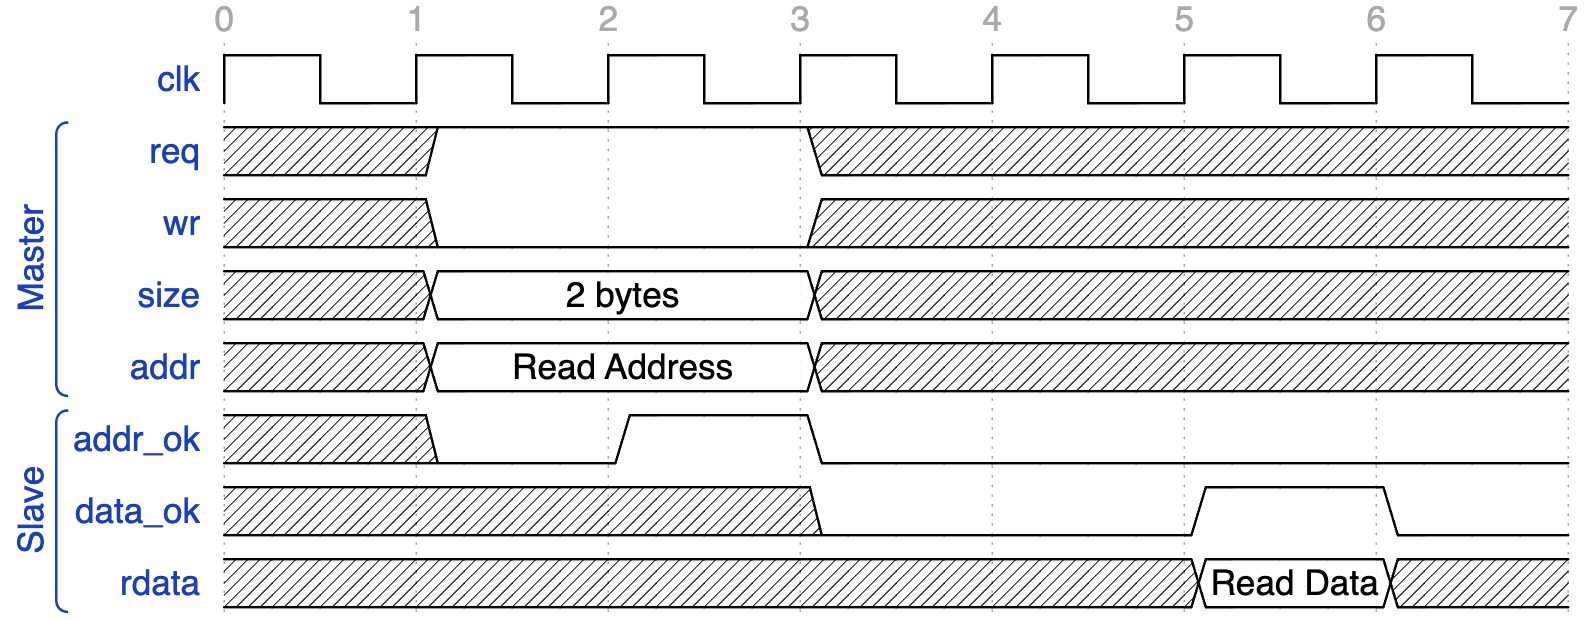
\includegraphics[width=1\linewidth]{assets/08/sram_read.jpg}
  \caption{类SRAM总线读事务时序图}
  \label{fig:sram-read}
\end{figure}

一次读事务可以被分解为几个关键步骤，每个步骤都发生在特定的时钟上升沿。

首先，在第一个时钟上升沿，主设备准备发起一个读请求。它通过设置请求信号\texttt{req}为高电平来通知从设备，同时将写请求信号\texttt{wr}保持在低电平，明确这是一个读操作而不是写操作。此时，主设备还会设置传输大小\texttt{size}为2 bytes，表明它希望读取两个字节的数据。

接着，在第二个时钟上升沿，主设备通过地址\texttt{addr}通道发送它想要读取的内存地址。这个地址被编码为特定的值，以便从设备能够识别和定位到正确的数据位置。此时，主设备和从设备尝试进行第一次握手。握手是通过地址确认信号\texttt{addr\_ok}来完成的。如果从设备成功接收并识别了地址，它会将\texttt{addr\_ok}信号设置为高电平，表示地址握手成功。然而，当前时刻握手失败了，所以在该时刻\texttt{addr\_ok}信号没有变为高电平，这可能是因为从设备需要额外的时间来准备或处理请求，无法单周期地接受请求数据。

到了第三个时钟上升沿，从设备准备好了，并通过将\texttt{addr\_ok}信号设置为高电平来确认地址握手成功。这意味着从设备已经接收并理解了主设备的请求，并且知道从哪个地址读取数据。

在接下来的两个时钟周期（第四和第五个时钟上升沿），主设备和从设备都在为数据传输做准备。主设备等待从设备将数据放到总线上，而从设备则在准备数据，以便在下一个时钟周期发送。在该过程中，从设备将数据握手信号\texttt{data\_ok}设置为低电平，即告知主设备读取请求仍在处理中，需要继续等待。

在第六个时钟上升沿，从设备完成了数据的读取，并通过读数据（\texttt{rdata}）信号将数据发送回主设备。同时，从设备设置数据确认信号（\texttt{data\_ok}）为高电平，表示数据握手成功，数据已经成功传输给主设备。

\subsubsection{写操作}\label{sec:08-bus-and-soc-007}

在类SRAM总线上进行一次写事务时的时序与读事务的类似。图\ref{fig:sram-write}展示了一个写操作的数据传输时序，与上面的读操作类似，但在时序细节上有所不同。

\begin{figure}[htbp]
  \centering
  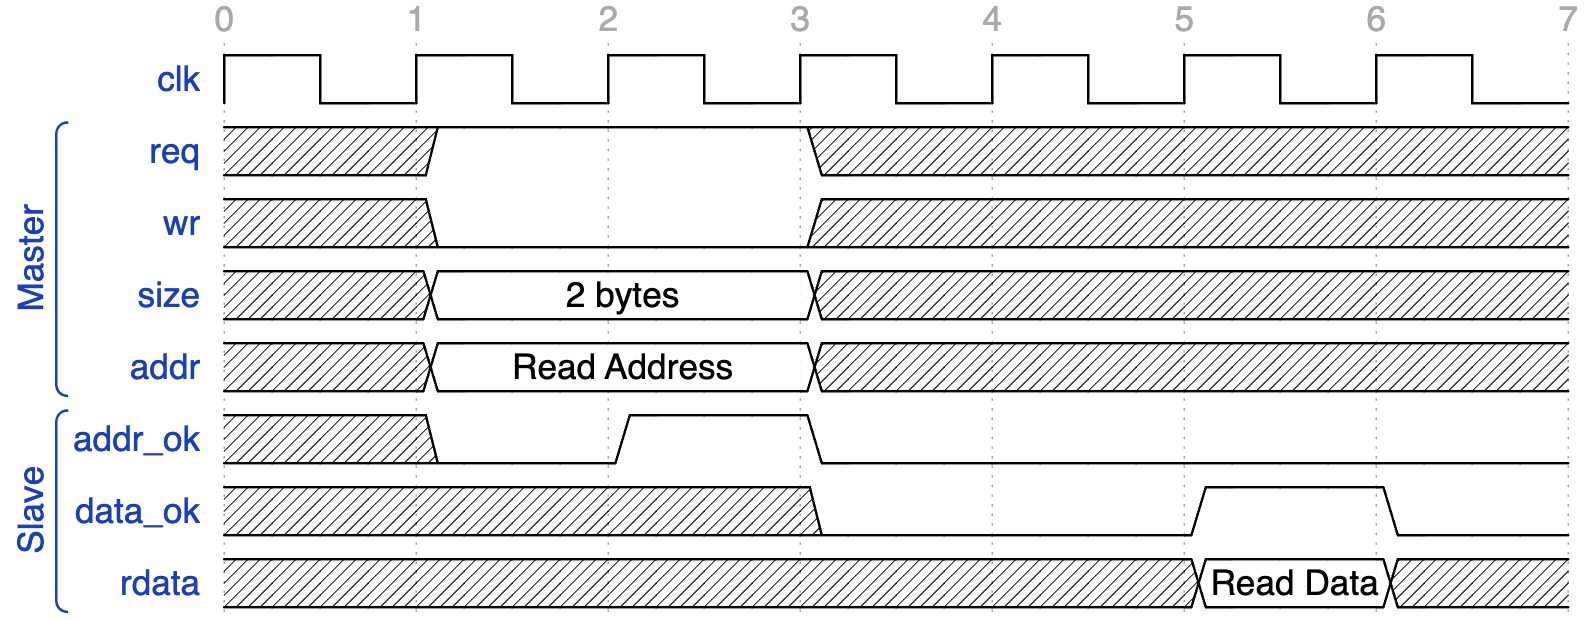
\includegraphics[width=1\linewidth]{assets/08/sram_write.jpg}
  \caption{类SRAM总线写事务时序图}
  \label{fig:sram-write}
\end{figure}

在第2个时钟上升沿，主端已设置好了写入的字节数\texttt{size}，写入地址\texttt{addr}和写入数据\texttt{wdata}，并将\texttt{wr}置高表示该事务为写事务，同时使用\texttt{req}通道向从方发送请求。

与上面读事务的时序图不同的是，在第2个时钟上升沿时，从方的\texttt{addr\_ok}直接为高电平，表示从方在单周期内成功接收了主方发送的所有数据信息。开发人员可以暂不关心从方具体是如何实现的，只需知道从方也可单周期接收数据，并在\texttt{req}置高的同时返回\texttt{addr\_ok}的握手信号。

在第二个时钟上升沿握手成功后，从方立即将\texttt{data\_ok}设置为低电平，告知主设备写入操作仍未完成。在等待三个周期后，在第6个时钟上升沿，\texttt{data\_ok}信号生效，从设备告知主设备写入完成。

至此，一次写操作结束。

\subsection{类SRAM总线的设计}\label{sec:08-bus-and-soc-008}

在类SRAM总线设计中，信号之间的约束关系直接影响总线的正确性和时序表现。以下是常见的约束和注意点：

\begin{itemize}
\tightlist
\item
  时序约束： \texttt{addr\_ok} 信号必须先于 \texttt{data\_ok} 激活，确保地址阶段先于数据阶段。
\item
  设计注意事项： 保持 \texttt{clk} 的稳定性是保证总线时序正确的基础；在高频率设计中，应特别关注信号传播延迟。
\end{itemize}

有些类SRAM总线协议包含特定要求。

作为开发者，在开发涉及类SRAM总线接口的功能时，需要仔细考虑这些信号的时序关系和协调。在发现总线相关的错误时，应当首先分析总线上握手信号和相关控制信号的波形，将主、从设备视为黑盒，分析是哪个设备执行出错，之后再进入下一个层次进行分析。尽量不要不区分层次地分析波形信号，因为在复杂CPU设计中信号层次很多，容易导致混乱。

在CPU设计中，类SRAM的各个控制信号的设计应根据具体的功能需求来优化：

\begin{itemize}
\tightlist
\item
  在取指令阶段，\texttt{addr\_ok} 的设计应确保地址信号能够在规定的时钟周期内传递到位，从而减少握手延迟。
\item
  在访存阶段 \texttt{data\_ok} 信号的设计应当灵活，以适应不同的数据大小传输需求。
\item
  优化时可使用流水线优化来提高数据吞吐量。
\item
  针对信号冲突，设计有效的仲裁机制，确保多主设备不会发生争用冲突。
\end{itemize}

\section{AXI总线协议}\label{sec:08-bus-and-soc-009}

AXI（Advanced eXtensible Interface）是一种广泛应用于现代片上系统（SoC）设计中的总线协议，它通过五个独立的通道实现主从设备之间的高效数据传输。每个通道可以独立工作，同时并发处理多个事务，这使得 AXI 总线在性能和灵活性上具有显著优势。

\subsection{接口信号}\label{sec:08-bus-and-soc-010}

AXI 协议将所有信号根据功能分为了五组，每组信号称为一个 \emph{通道}：读地址通道（Read Address Channel，AR），读数据通道（Read Data Channel，R），写地址通道（Write Address Channel，AW），写数据通道（Write Data Channel，W）以及写响应通道（Write Response Channel，B）。这五个通道负责处理从主设备到从设备的请求与响应过程，每个通道都有独特的信号集。

图\ref{fig:axi-channels}展示了AXI接口中的五个通道。读地址通道AR用于将主方希望读取的地址传输给从方，而从方读取到的数据将通过读数据通道R返回给主方。对于写操作，主方将写入地址及写入数据分别通过写地址通道AW和写数据通道W传输给从方，从方使用写响应通道B将是否正确写入的信息传输给主方。

\begin{figure}[htbp]
  \centering
  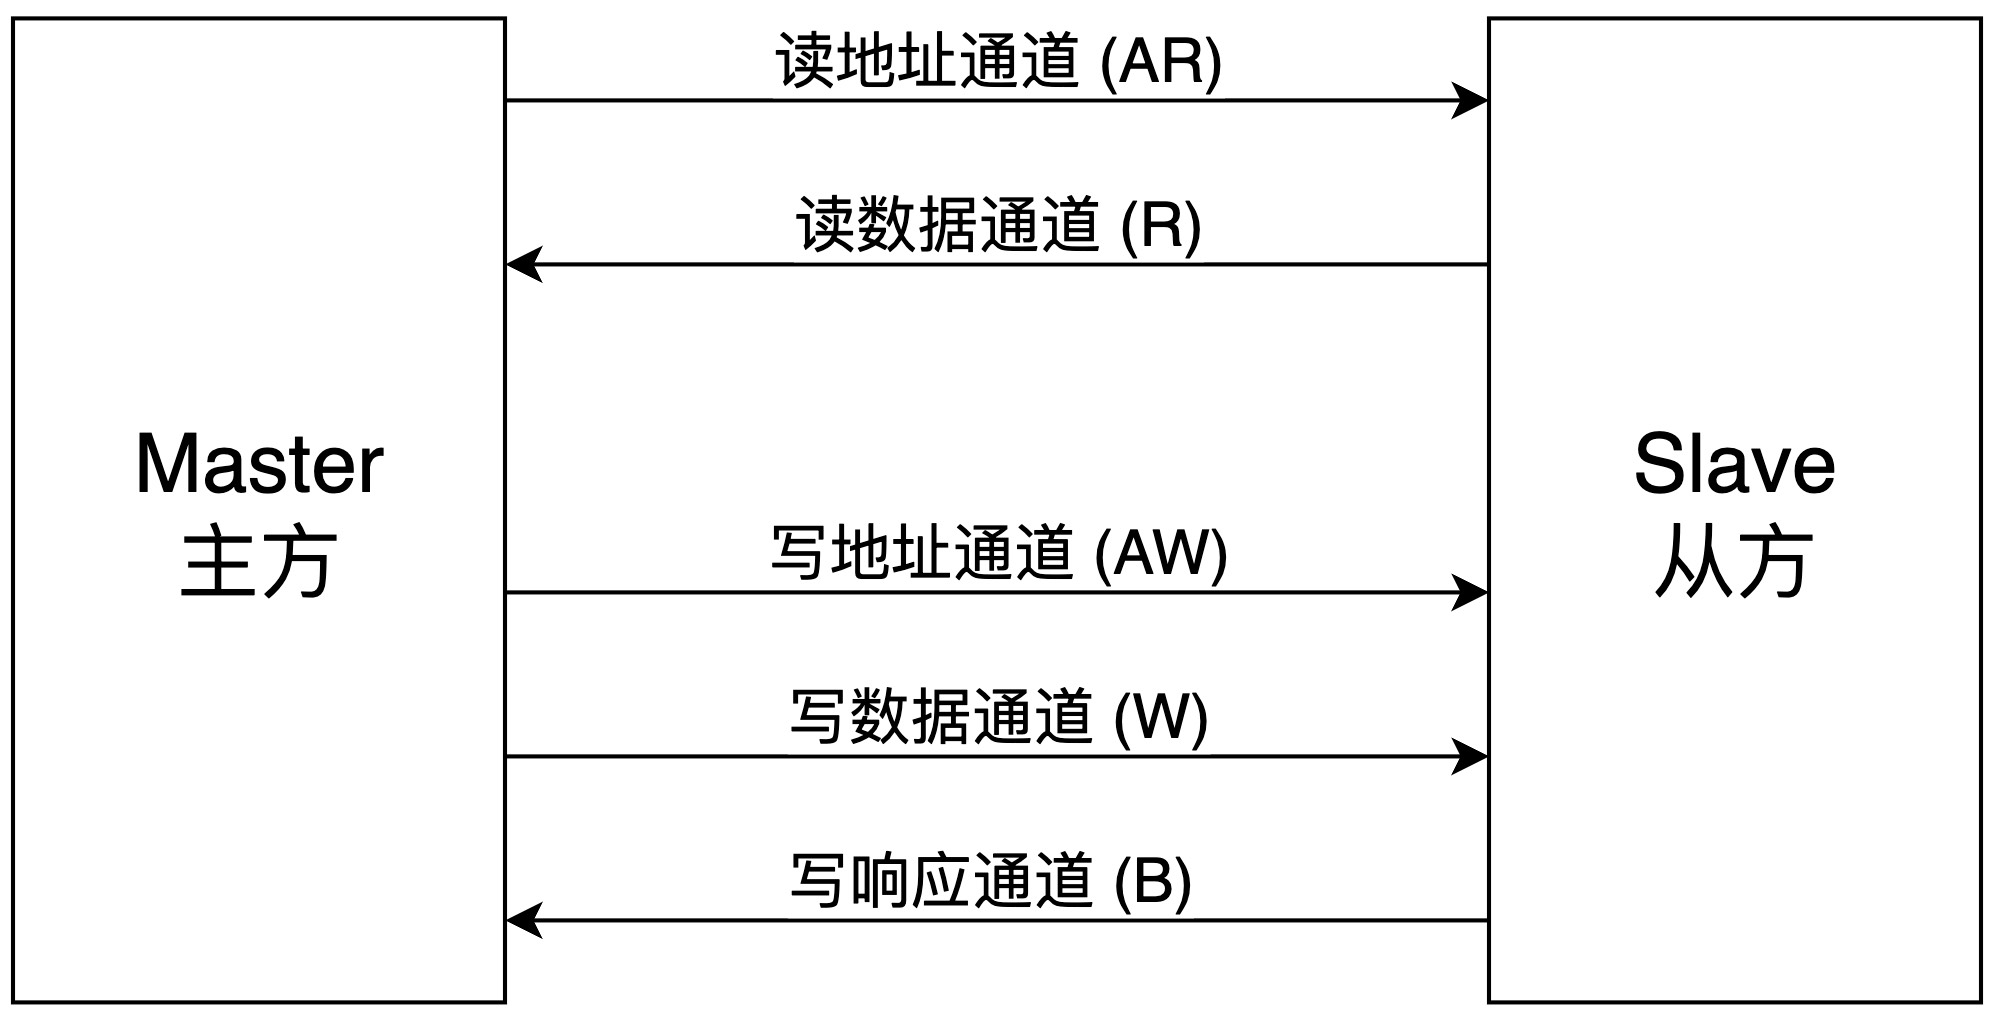
\includegraphics[width=0.7\linewidth]{assets/08/axi_channels.jpg}
  \caption{AXI总线通道示意图}
  \label{fig:axi-channels}
\end{figure}

应当注意的是，该图中的箭头方向指的是\textbf{数据流动的方向}，而并不直接表示信号的输入输出方向。每个通道内，均有从主方到从方以及从从方到主方的信号线路。例如，读地址通道用于将主方希望读取的地址通知从方，但从方也需要通过一些控制信号告知主方，主方传递的地址已收到，因此在该通道内仍需要由从方到主方的信号。这种用于确认对方是否正确接收好数据的信号称为 \emph{握手信号}，下面的某些小节将详细介绍AXI总线中的握手方法。

\subsubsection{读地址通道 (AR)}\label{sec:08-bus-and-soc-011}

\begin{longtable}[]{@{}
  >{\raggedright\arraybackslash}p{(\linewidth - 6\tabcolsep) * \real{0.1412}}
  >{\raggedright\arraybackslash}p{(\linewidth - 6\tabcolsep) * \real{0.1294}}
  >{\raggedright\arraybackslash}p{(\linewidth - 6\tabcolsep) * \real{0.2235}}
  >{\raggedright\arraybackslash}p{(\linewidth - 6\tabcolsep) * \real{0.5059}}@{}}
\toprule\noalign{}
\begin{minipage}[b]{\linewidth}\raggedright
信号
\end{minipage} & \begin{minipage}[b]{\linewidth}\raggedright
位宽
\end{minipage} & \begin{minipage}[b]{\linewidth}\raggedright
方向
\end{minipage} & \begin{minipage}[b]{\linewidth}\raggedright
功能
\end{minipage} \\
\midrule\noalign{}
\endhead
\bottomrule\noalign{}
\endlastfoot
ARID & 4-16 bits & Master → Slave & 传输读请求的标识符，用于区分不同的事务 \\
ARADDR & 32-64 bits & Master → Slave & 传输读地址，指示从何处读取数据 \\
ARLEN & 4 bits & Master → Slave & 传输突发传输的长度，指示读取多少个数据字 \\
ARSIZE & 3 bits & Master → Slave & 传输数据的大小，表示每个传输的数据字节数 \\
ARBURST & 2 bits & Master → Slave & 传输突发传输类型，支持递增、包装和固定 \\
ARVALID & 1 bit & Master → Slave & 表示读地址有效，启动握手 \\
ARREADY & 1 bit & Slave → Master & 表示从设备已准备好接收读地址 \\
\end{longtable}

\textbf{重点信号说明：}

\begin{itemize}
\item
  \textbf{ARID}：用于区分主设备发起的多个并发读请求。每个请求的 ARID 唯一标识该请求。
\item
  \textbf{ARADDR}：传输内存地址，主设备发出读请求时，需要指定从哪个地址读取数据。
\item
  \textbf{ARVALID 与 ARREADY}：ARVALID 表示主设备的地址和控制信号有效，而 ARREADY 则是从设备的响应信号，当二者同时为高时，地址握手完成。
\end{itemize}

\subsubsection{读数据通道 (R)}\label{sec:08-bus-and-soc-012}

\begin{longtable}[]{@{}
  >{\raggedright\arraybackslash}p{(\linewidth - 6\tabcolsep) * \real{0.1412}}
  >{\raggedright\arraybackslash}p{(\linewidth - 6\tabcolsep) * \real{0.1294}}
  >{\raggedright\arraybackslash}p{(\linewidth - 6\tabcolsep) * \real{0.2235}}
  >{\raggedright\arraybackslash}p{(\linewidth - 6\tabcolsep) * \real{0.5059}}@{}}
\toprule\noalign{}
\begin{minipage}[b]{\linewidth}\raggedright
信号
\end{minipage} & \begin{minipage}[b]{\linewidth}\raggedright
位宽
\end{minipage} & \begin{minipage}[b]{\linewidth}\raggedright
方向
\end{minipage} & \begin{minipage}[b]{\linewidth}\raggedright
功能
\end{minipage} \\
\midrule\noalign{}
\endhead
\bottomrule\noalign{}
\endlastfoot
RID & 4-16 bits & Slave → Master & 传输读请求的标识符，表示正在返回哪个事务的数据 \\
RDATA & 32-64 bits & Slave → Master & 传输读到的数据 \\
RRESP & 2 bits & Slave → Master & 传输读数据的响应状态（OKAY、ERROR等） \\
RLAST & 1 bit & Slave → Master & 表示这是突发传输的最后一个数据字 \\
RVALID & 1 bit & Slave → Master & 表示读数据有效，启动握手 \\
RREADY & 1 bit & Master → Slave & 表示主设备已准备好接收读数据 \\
\end{longtable}

\textbf{重点信号说明：}

\begin{itemize}
\item
  \textbf{RDATA}：主设备从从设备读取的数据，通过该信号传递给主设备。
\item
  \textbf{RLAST}：当进行突发传输时，RLAST 表示突发传输的最后一个数据字。
\item
  \textbf{RVALID 与 RREADY}：当 RVALID 为高时，表示从设备传输的数据有效；RREADY 为高时，表示主设备准备好接收数据。
\end{itemize}

\subsubsection{写地址通道 (AW)}\label{sec:08-bus-and-soc-013}

\begin{longtable}[]{@{}
  >{\raggedright\arraybackslash}p{(\linewidth - 6\tabcolsep) * \real{0.1412}}
  >{\raggedright\arraybackslash}p{(\linewidth - 6\tabcolsep) * \real{0.1294}}
  >{\raggedright\arraybackslash}p{(\linewidth - 6\tabcolsep) * \real{0.2235}}
  >{\raggedright\arraybackslash}p{(\linewidth - 6\tabcolsep) * \real{0.5059}}@{}}
\toprule\noalign{}
\begin{minipage}[b]{\linewidth}\raggedright
信号
\end{minipage} & \begin{minipage}[b]{\linewidth}\raggedright
位宽
\end{minipage} & \begin{minipage}[b]{\linewidth}\raggedright
方向
\end{minipage} & \begin{minipage}[b]{\linewidth}\raggedright
功能
\end{minipage} \\
\midrule\noalign{}
\endhead
\bottomrule\noalign{}
\endlastfoot
AWID & 4-16 bits & Master → Slave & 传输写请求的标识符 \\
AWADDR & 32-64 bits & Master → Slave & 传输写地址，指示将数据写入哪个地址 \\
AWLEN & 4 bits & Master → Slave & 传输突发传输的长度 \\
AWSIZE & 3 bits & Master → Slave & 传输数据大小，表示每次传输的数据字节数 \\
AWBURST & 2 bits & Master → Slave & 传输突发类型（递增、包装或固定） \\
AWVALID & 1 bit & Master → Slave & 表示写地址有效，启动握手 \\
AWREADY & 1 bit & Slave → Master & 表示从设备已准备好接收写地址 \\
\end{longtable}

\textbf{重点信号说明：}

\begin{itemize}
\item
  \textbf{AWADDR}：与读地址通道类似，AWADDR 传输写地址，指定要写入的内存地址。
\item
  \textbf{AWLEN}：指示突发传输的总长度，即一次写操作要写入的总数据字个数。
\item
  \textbf{AWVALID 与 AWREADY}：类似于读通道的握手信号，AWVALID 表示写地址有效，AWREADY 则表示从设备准备好接收写地址。
\end{itemize}

\subsubsection{写数据通道 (W)}\label{sec:08-bus-and-soc-014}

\begin{longtable}[]{@{}
  >{\raggedright\arraybackslash}p{(\linewidth - 6\tabcolsep) * \real{0.1412}}
  >{\raggedright\arraybackslash}p{(\linewidth - 6\tabcolsep) * \real{0.1294}}
  >{\raggedright\arraybackslash}p{(\linewidth - 6\tabcolsep) * \real{0.2235}}
  >{\raggedright\arraybackslash}p{(\linewidth - 6\tabcolsep) * \real{0.5059}}@{}}
\toprule\noalign{}
\begin{minipage}[b]{\linewidth}\raggedright
信号
\end{minipage} & \begin{minipage}[b]{\linewidth}\raggedright
位宽
\end{minipage} & \begin{minipage}[b]{\linewidth}\raggedright
方向
\end{minipage} & \begin{minipage}[b]{\linewidth}\raggedright
功能
\end{minipage} \\
\midrule\noalign{}
\endhead
\bottomrule\noalign{}
\endlastfoot
WDATA & 32-64 bits & Master → Slave & 传输要写入的数据 \\
WSTRB & 4-8 bits & Master → Slave & 数据写入时的字节掩码，指示哪些字节有效 \\
WLAST & 1 bit & Master → Slave & 表示突发传输中的最后一个数据字 \\
WVALID & 1 bit & Master → Slave & 表示写数据有效，启动握手 \\
WREADY & 1 bit & Slave → Master & 表示从设备已准备好接收写数据 \\
\end{longtable}

\textbf{重点信号说明：}

\begin{itemize}
\item
  \textbf{WDATA}：主设备要写入从设备的数据通过该信号传递。
\item
  \textbf{WSTRB}：写数据时的字节掩码，用于指示哪些字节有效，这在非对齐或部分写操作中尤为重要。
\item
  \textbf{WLAST}：当进行突发传输时，WLAST 信号用于指示写数据的最后一个数据字。
\end{itemize}

\subsubsection{写响应通道 (B)}\label{sec:08-bus-and-soc-015}

\begin{longtable}[]{@{}
  >{\raggedright\arraybackslash}p{(\linewidth - 6\tabcolsep) * \real{0.1412}}
  >{\raggedright\arraybackslash}p{(\linewidth - 6\tabcolsep) * \real{0.1294}}
  >{\raggedright\arraybackslash}p{(\linewidth - 6\tabcolsep) * \real{0.2235}}
  >{\raggedright\arraybackslash}p{(\linewidth - 6\tabcolsep) * \real{0.5059}}@{}}
\toprule\noalign{}
\begin{minipage}[b]{\linewidth}\raggedright
信号
\end{minipage} & \begin{minipage}[b]{\linewidth}\raggedright
位宽
\end{minipage} & \begin{minipage}[b]{\linewidth}\raggedright
方向
\end{minipage} & \begin{minipage}[b]{\linewidth}\raggedright
功能
\end{minipage} \\
\midrule\noalign{}
\endhead
\bottomrule\noalign{}
\endlastfoot
BID & 4-16 bits & Slave → Master & 传输写事务的标识符 \\
BRESP & 2 bits & Slave → Master & 传输写操作的响应状态 \\
BVALID & 1 bit & Slave → Master & 表示写响应有效，启动握手 \\
BREADY & 1 bit & Master → Slave & 表示主设备已准备好接收写响应 \\
\end{longtable}

\textbf{重点信号说明：}

\begin{itemize}
\item
  \textbf{BRESP}：传输写操作的结果状态（如 OKAY、ERROR），用于指示写操作是否成功完成。
\item
  \textbf{BVALID 与 BREADY}：BVALID 表示从设备传输的响应有效，BREADY 则表示主设备已准备好接收响应。
\end{itemize}

\subsection{握手机制}\label{sec:08-bus-and-soc-016}

在每个通道内，AXI均设计了一对握手信号，即\texttt{VALID}和\texttt{READY}。在不同的通道中，这些握手信号将以通道名+\texttt{VALID}或\texttt{READY}的形式命名。因此，AXI总线共含有5对握手信号。例如，在B通道内，握手信号的名称为\texttt{BVALID}和\texttt{BREADY}。

AXI 的握手机制就通过每个通道内的握手信号完成。每个通道是独立的一组信息传递单元，每个通道内的握手信号控制了该通道内所有数据的传输。AXI总线上复杂的信息传输，是通过五个通道内的信息传输所构成的。

握手机制的关键在于，只有当该通道的 \texttt{VALID} 和 \texttt{READY} 信号都为高时，数据传输才会发生。
例如，图\ref{fig:axi-handshake}展示了读地址通道的握手时序。

\begin{figure}[htbp]
  \centering
  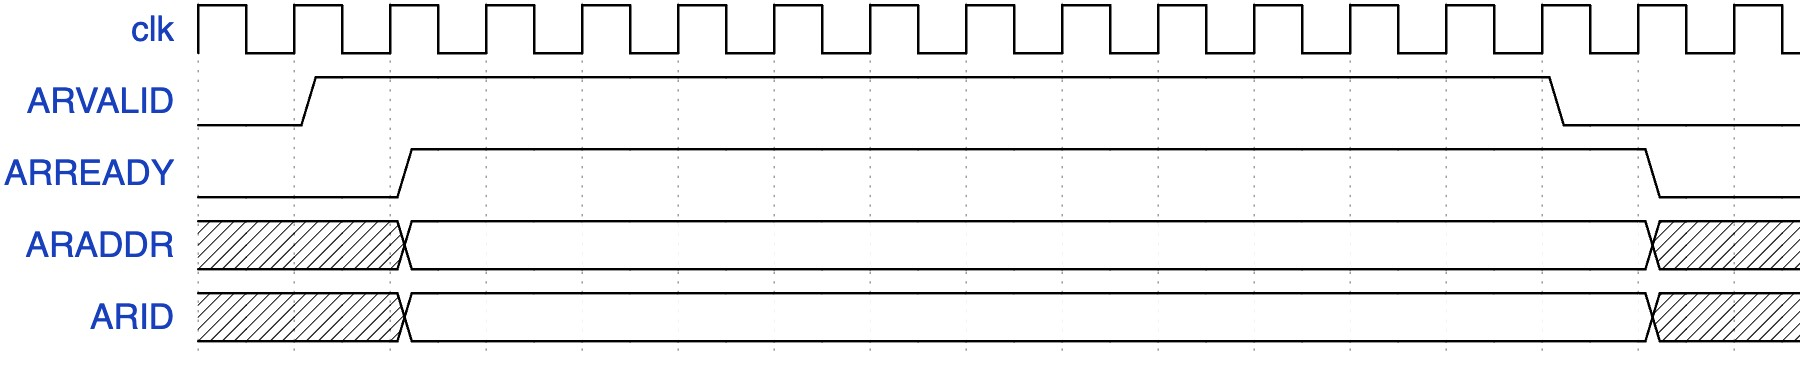
\includegraphics[width=1\linewidth]{assets/08/axi_handshake.jpg}
  \caption{AXI总线AR端口握手信号时序图}
  \label{fig:axi-handshake}
\end{figure}

在时钟上升沿时，如果 ARVALID 和 ARREADY 同时为高，表示主从设备之间的握手完成，地址传输成功。

\subsection{总线事务}\label{sec:08-bus-and-soc-017}

AXI总线事务通常由多个握手过程组合完成。读事务和写事务分别通过不同的通道进行通信。

\subsubsection{读事务}\label{sec:08-bus-and-soc-018}

完整的读事务包括一次读地址通道的握手和一次读数据通道的握手。在读事务开始时，主设备通过 AR 通道传输地址信息，随后从设备在 R 通道上返回数据。在AR通道内和R通道内的数据传输中，分别需要一次握手，即\texttt{VALID}和\texttt{READY}信号同时生效时产生的数据传输。

图\ref{fig:axi-read}展示了AXI总线的一次读事务的完整过程，其中有些信号被省略。

\begin{figure}[htbp]
  \centering
  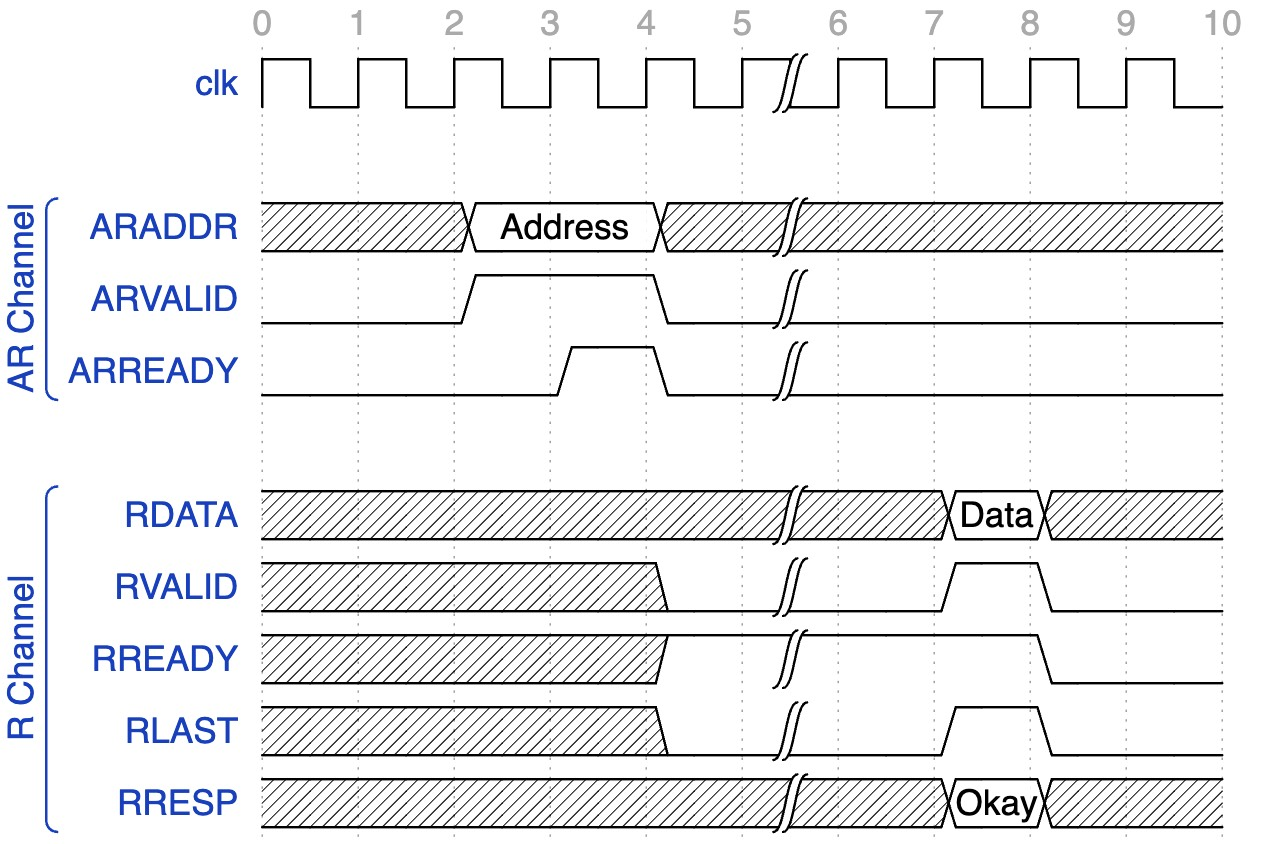
\includegraphics[width=1\linewidth]{assets/08/axi_read.jpg}
  \caption{AXI总线读事务时序图}
  \label{fig:axi-read}
\end{figure}

在上述时序图中，第2个时钟上升沿之后，ARVALID 生效，表示主设备已通过ARADDR通道准备好发送读地址。
在第3个时钟上升沿时，ARREADY为低电平，表示从设备没有准备好接收，于是主设备继续维持ARADDR不变，并持续将ARVALID置高。

在第4个时钟上升沿时，ARREADY被从方置高。此时，ARVALID和ARREADY同时生效，说明AR通道握手成功，即从设备已经接受了ARADDR信号表示的读地址，以及其他一些读取设置参数（这些信号在本图中被省略）。

下面，从设备应当通过R通道，向主设备发送读取到的数据。由于从设备在接受好读地址之后，可能需要一定的时间才能成功获取数据，因此RVALID将首先被从方设置为低电平。同时，由于主方已经做好了接受数据的准备，因此它将RREADY在第5个时钟上升沿置高。实际情况中，主方有可能并不会在AR通道握手成功后，立刻将RREADY置高，因为可能需要一定时间才能完成接受数据的准备。

在之后的一段时间内，主设备等待从设备进行数据的读取。

在图中的第8个时钟上升沿时，从设备将读取数据准备好，并将RDATA数据设置为正确的值。与此同时，将RVALID置高。
此时，R通道成功握手。
在此图中RLAST信号也为高，说明该数据是本组传输的最后一个数据。
在突发传输模式中，该信号具有重要的用途。后文将详细介绍。

\subsubsection{写事务}\label{sec:08-bus-and-soc-019}

写事务包括三次握手，分别为写地址（AW）、写数据（W）、写响应（B）通道的握手。主设备先通过 AW 通道传输写地址，随后通过 W 通道传输写数据，最后从设备通过 B 通道返回写操作的响应。在整个过程中，需要三次握手，分别对应三个通道的数据传输。

图\ref{fig:axi-write}展示了AXI总线的一次写事务的完整过程，其中有些信号被省略。

\begin{figure}[htbp]
  \centering
  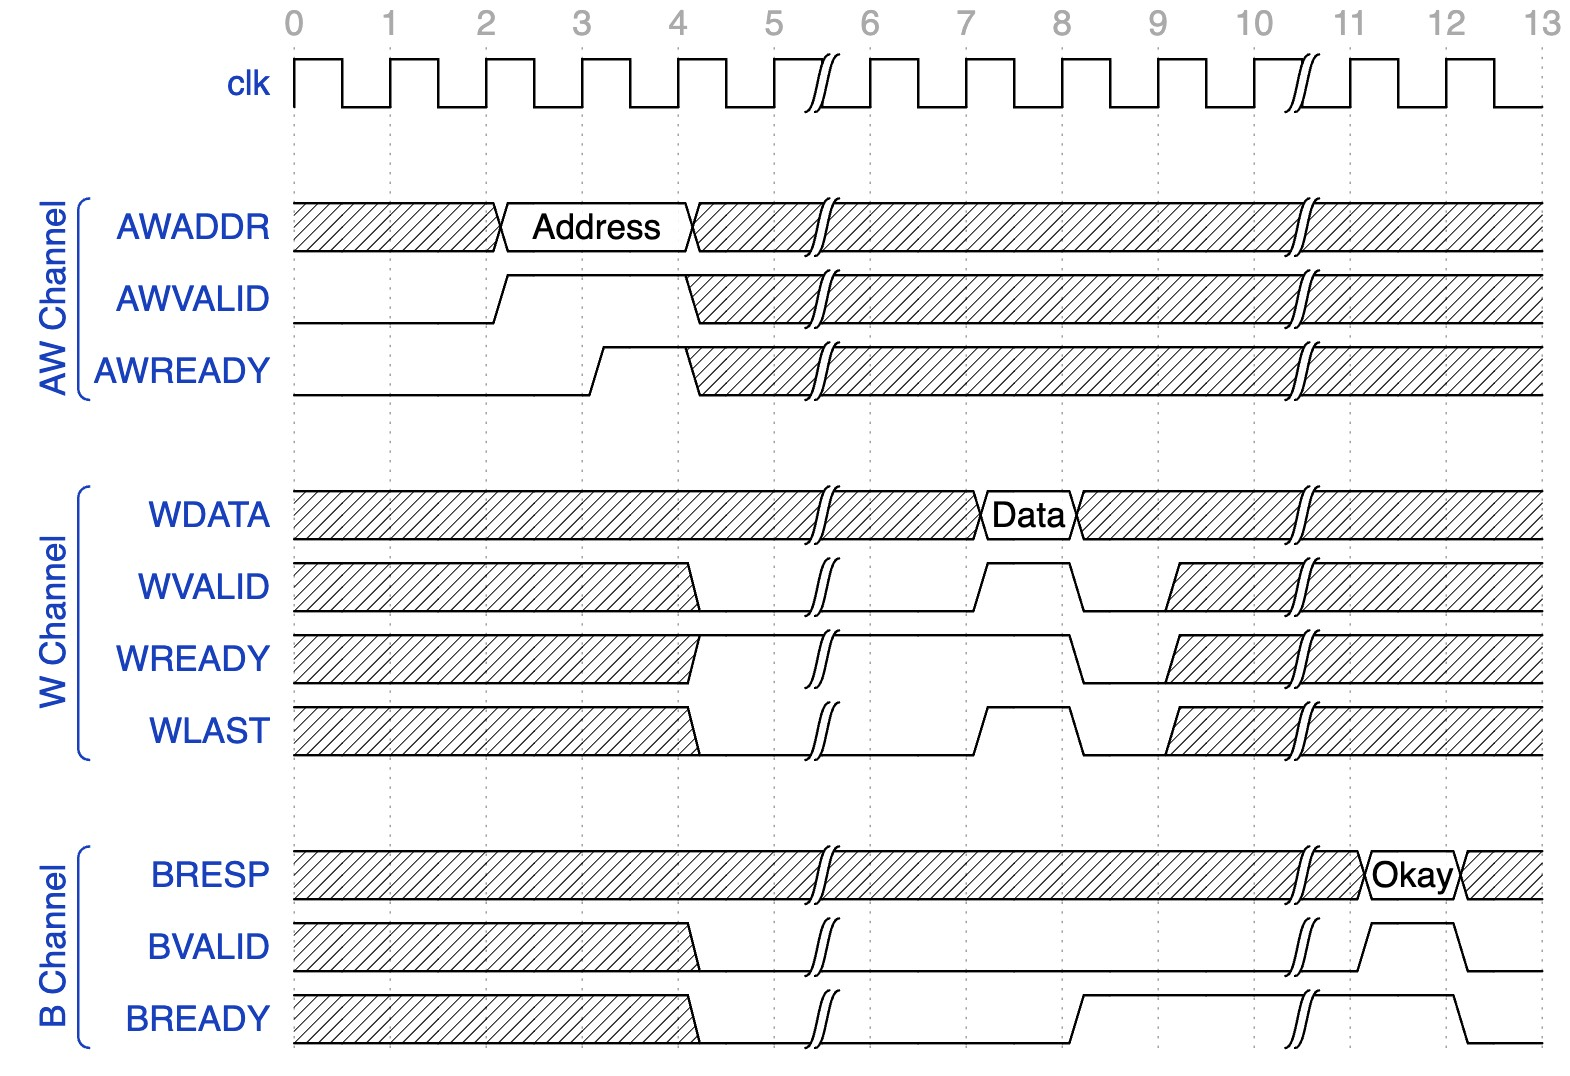
\includegraphics[width=1\linewidth]{assets/08/axi_write.jpg}
  \caption{AXI总线写事务时序图}
  \label{fig:axi-write}
\end{figure}

从图中可以看出，总共有AW、W、B三个通道参与了信息传递。

在前5个时钟周期，AW通道进行了地址的传输，告知了从方待写入的地址。具体的握手过程与上小节介绍的在读事务中AR通道进行的地址传输基本相同。在第4个时钟上升沿，完成了握手。

之后，主方将通过W通道，将待写入的数据发送给从方。从方先将WREADY设置为1，表示从方已做好准备接受写入的数据。然而，此时主方并没有准备好数据，因此WVALID一直为0，此时从方需要等待。在第8个时钟上升沿，WVALID为高，表示数据已经在WDATA信号中准备好。同时WLAST为1，表示该数据为本组传输中最后一个数据（其他使用方法见突发传输一节）。至此，从方已经接受了主方发送的全部信息，包括待写入的地址和数据。在本图中忽略的其他信号中，主方还进行了写入字节数等设置。

此时从方可以开始完成数据的写入工作，并且需要在写入完成后，将写入结果通过B通道发送给主方，告知是否写入成功。在写入正在进行时，从方将BVALID设置为0，而BREADY由主方设置为1，表明主方时刻做好了接受写入结果信息的准备，但从方仍在进行写入工作，或者写入工作进行完成但没有准备好结果信息的数据。在其他的情况中，可能BREADY会被置为0，这表明主方没有做好接受写入结果信息的准备。本图只表示所有可能情况中的一种，开发人员需要根据具体情况进行分析。

在第12个时钟上升沿，从方将Okay消息传输给从方，并在B通道成功握手。此时，一次写事务成功完成。从方也可能会将错误信息通过B通道传递给主方，表示写入失败，这种情况下主方需要进行一些错误处理，例如重传。

\subsection{突发传输模式}\label{sec:08-bus-and-soc-020}

在AXI总线中，\textbf{突发传输模式（burst mode）}是一种能够提高数据传输效率的方式。突发传输允许主设备（Master）发出一次地址请求，随后从设备（Slave）在不需要额外地址请求的情况下，连续传输多个数据。这样可以减少每次传输地址带来的延迟，大幅提高数据带宽，特别适合缓存、内存等连续读写场景。

\subsubsection{突发传输类型}\label{sec:08-bus-and-soc-021}

AXI协议支持三种不同的突发传输类型：

\begin{enumerate}
\def\labelenumi{\arabic{enumi}.}
\item
  \textbf{固定突发（Fixed Burst）}：所有传输使用相同的地址。适用于外设寄存器读取等场景。
\item
  \textbf{增量突发（Incrementing Burst）}：每次传输地址递增，适合连续存储器读取操作。地址按照数据位宽自动递增，例如每次传输32位数据时，地址增量为4字节。
\item
  \textbf{环形突发（Wrapping Burst）}：在传输过程中，当达到指定的最大地址时，地址将回绕到起始地址。常用于支持关键字优先的缓存操作，即在一个cache行中，先读取当前CPU流水线所需要的数据，并且立即返回给CPU流水线，在流水线继续工作的同时，再继续读取该cache行中其他位置的数据并存入cache中。AXI的环形突发模式可以很完美的适配于关键字优先技术。
\end{enumerate}

突发传输的长度可以是1到256个数据拍（beat）。主设备通过 ARLEN 或 AWLEN 信号指定传输的长度。

\subsubsection{突发传输的时序}\label{sec:08-bus-and-soc-022}

\begin{figure}[htbp]
  \centering
  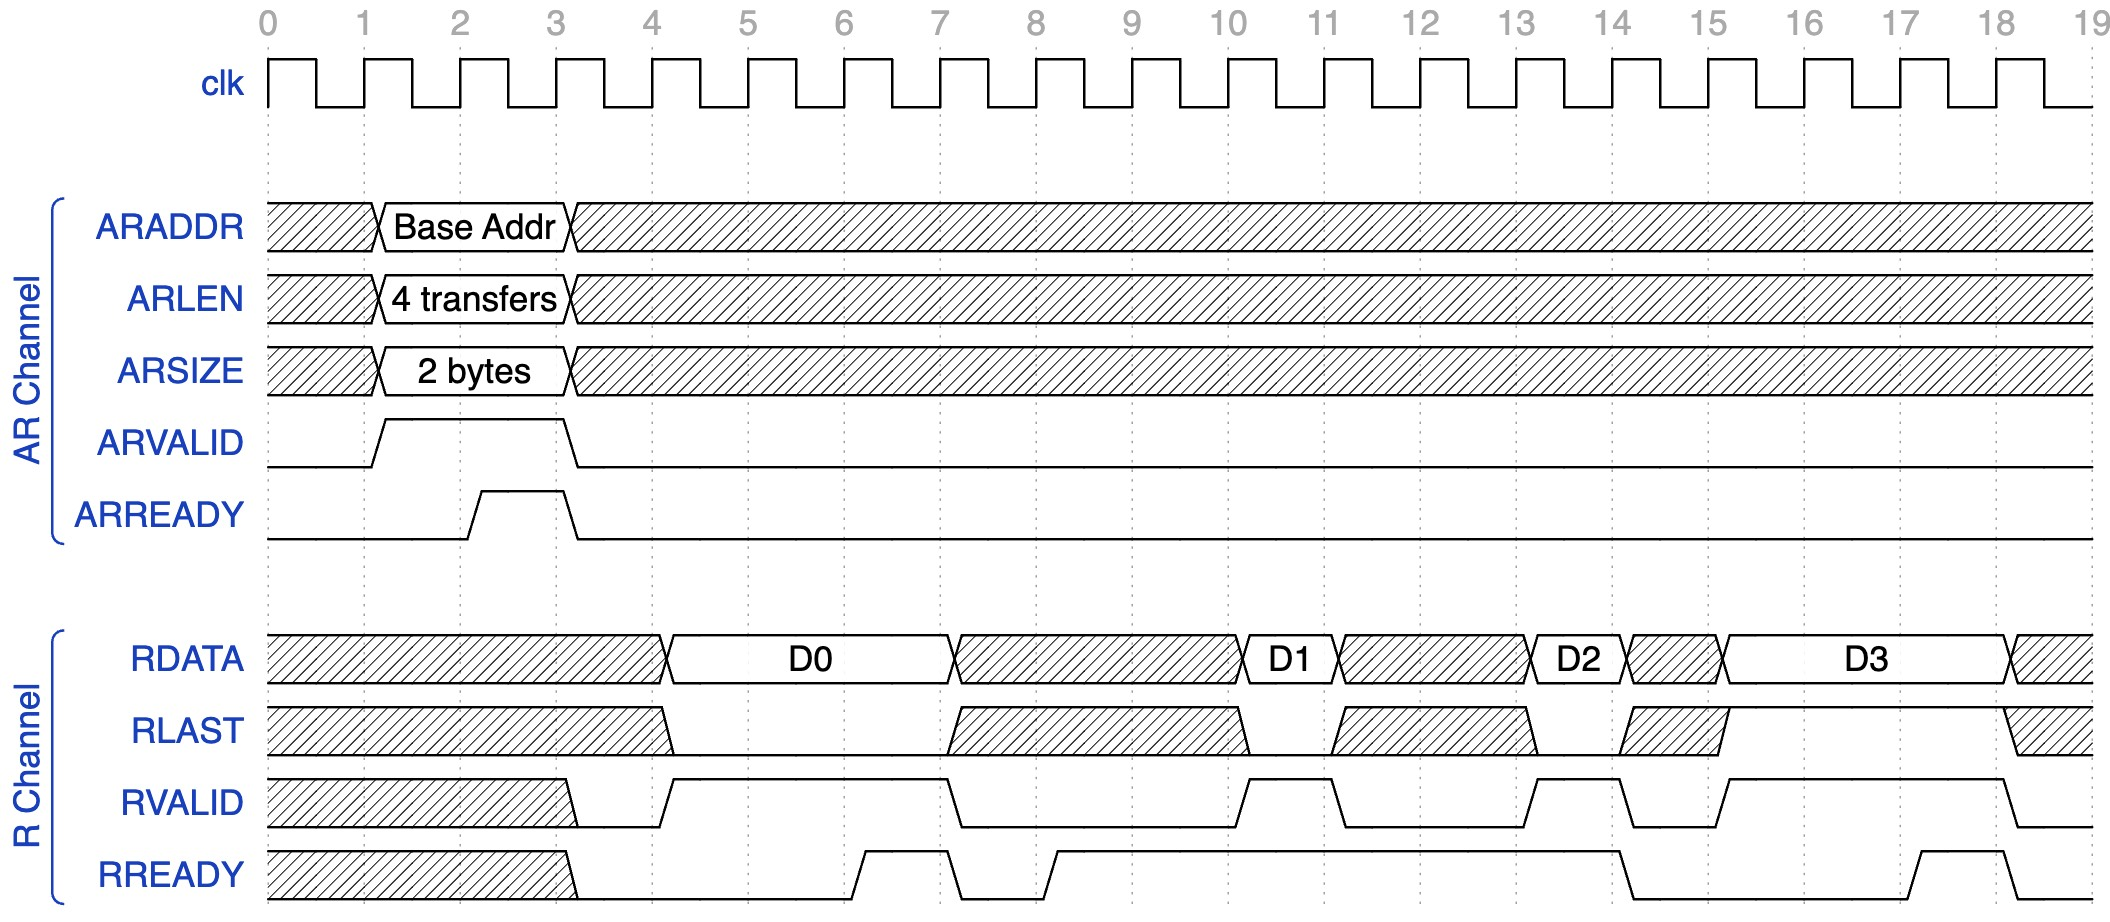
\includegraphics[width=1\linewidth]{assets/08/axi_burst.jpg}
  \caption{AXI总线突发传输读事务时序图}
  \label{fig:axi-burst}
\end{figure}

图\ref{fig:axi-burst}展示了AXI总线的突发传输模式中，一次读事务的时序图。

突发传输模式是在主方通过AR通道发送读请求，或者通过AW通道发送写请求时，通过\texttt{ARLEN/AWLEN}和\texttt{ARBURST/AWBURST}设置的。\texttt{ARLEN/AWLEN}设置了本次读/写事务中的数据传输次数，在本图中主方设置为了4，表示在本次读事务中需要连续传输4次数据。\texttt{ARBURST/AWBURST}设置了本次读/写事务的类型，包括上小节提到的三种，该信号在本图中被省略，从方将根据该配置信息决定在本次的读/写事务中，每次发送/接受的数据地址该如何变化（例如全部使用相同地址、地址递增、或者环形增加）。

在图中的第3个时钟上升沿，AR通道完成了握手。\texttt{ARSIZE}设置的是一次数据传输将传输2字节的数据，\texttt{ARADDR}设置了本次突发传输的基地址。因此，从方将通过R通道向主方发送以\texttt{ARADDR}地址为首地址的数据，每次数据传输将发送2字节数据，总共含有4次数据传输。因此，在本次读事务中将读取共8字节的数据。

在每次只能最多传输2字节的情况下，若不使用突发传输，传输共8字节的数据需要主方发起4次读事务，这表示主方需要通过AR通道发送4次地址信息，而从方需要通过R通道发送4次数据信息。在本图所示的突发传输模式下，主方只需要通过AR通道发送1次地址信息，同时进行突发传输模式配置，之后从方可连续地通过R通道发送4次数据信息，减少了AR通道的3次握手。由于一次读取的数据块更大，因此从方设备可能也能更快的作出响应，提高了总线效率。

在第4到第7个时钟上升沿中，从方通过R通道发送了第一个数据\(D0\)，并将RVALID置高，同时将RLAST置低。RLAST信号表示当前发送的数据是否为本此读事务的最后一次数据传输。本次读事务总共需要完成4次数据传输，因此此时传输的第一个数据不是最后一次数据传输，因此RLAST为0。由于一开始主方并未做好接受准备，因此RREADY在4-6个时钟上升沿时都为0，并在第7个时钟上升沿成功握手。

在第9个时钟上升沿，主方设备做好了接受准备，但从方并没有完成数据的读取，因此RVALID为低但RREADY为高，主方等待从方传输数据。在第11个时钟上升沿，第二个数据\(D1\)成功握手，RLAST也为0。同理，在第14个时钟上升沿，完成了第三个数据传输。

从第16个时钟上升沿开始，从方开始在RDATA发送最后一组数据\(D3\)，同时将RLAST置高，告知主方在本次数据传输结束后，本次读事务将结束。在第18个时钟上升沿时成功握手，标志着最后一组数据的成功传输，以及本次读事务的结束。

\subsubsection{突发传输的应用和实现}\label{sec:08-bus-and-soc-023}

突发传输特别适合缓存设计。例如，处理器从主内存读取数据时，通常以块的形式读取多个连续地址的内容。突发模式允许一次性传输整个数据块，减少了多个单独请求的开销。突发传输的另一个应用场景是DMA（直接内存访问）操作。DMA传输通常涉及大量数据的连续传输，突发传输能够极大提高DMA通道的效率，减少系统总线的占用时间。

在CPU实现过程中，应尽量选择适合数据块大小的突发长度，以充分利用传输带宽。例如，对于缓存行大小为64字节的系统，可以选择传输8个32位的数据拍。另外，应尽量减少突发传输之间的间隔时间，确保数据连续传输，避免总线资源浪费。

\subsection{其他总线特性}\label{sec:08-bus-and-soc-024}

AXI 总线还具有其他显著的特性，例如并发访问、乱序响应和 ID 信号的使用。以下将详细介绍这些特性。

AXI 总线允许\textbf{并发访问}，这意味着不同的事务可以同时在多个通道中进行。主设备能够在多个通道中并发发起地址、数据和响应传输，而从设备则通过握手机制协调这些并发事务。例如，主设备可以在发起写事务的同时发起另一个读事务。AXI 总线的并发特性提高了数据传输的效率，使系统能够更好地利用带宽资源。

\textbf{乱序响应}是 AXI 总线的一大优势，它允许从设备以不同于请求顺序的方式响应主设备的请求。这种灵活性使得 AXI 总线在处理复杂的、多线程操作时表现出色。然而，乱序响应也带来了系统设计上的挑战，设计者需要确保主设备能够正确地管理这些乱序响应，避免数据的混淆。

AXI 总线中的 \textbf{ID 信号}为事务的识别提供了重要支持。每个事务可以携带一个唯一的 ID 标识符，用来区分不同事务或线程的请求。这对于处理多线程的并行操作非常有用，特别是在一个主设备发起多个请求时，ID 可以确保从设备能正确识别和响应每一个事务。

\section{类SRAM总线与AXI总线桥接设计}\label{sec:08-bus-and-soc-025}

在设计计算机系统时，类SRAM总线与AXI总线的桥接设计是非常重要的一环。它不仅能够确保两种不同总线系统之间的互操作性，还可以提高系统整体的性能和可靠性。类SRAM总线较为简洁，因此可以用作内部设计时的接口。而AXI性能较高，有多种高性能传输特性，功能全面，适合作为片上总线，连接SoC上的不同设备。因此，往往需要设计类SRAM总线与AXI总线的转接桥。
在桥接设计中，关键任务之一是将两种总线的接口信号正确映射和转换，保证它们之间的数据传输和控制流的正确进行。

\subsection{类SRAM总线接口信号和AXI总线接口信号的关系}\label{sec:08-bus-and-soc-026}

类SRAM总线通常用于片上系统，信号较为简洁。主要信号包括请求信号req，地址信号addr，数据握手信号addr\_ok和data\_ok，以及读/写数据信号。而AXI总线作为一种更复杂的总线协议，定义了多个通道，分别处理地址、数据和响应等信息。在AXI协议中，关键信号包括地址写通道AWVALID和AWREADY，数据写通道WVALID和WREADY，以及响应通道BVALID和BREADY。类似的读操作则有ARVALID、ARREADY（地址通道）和RVALID、RREADY（数据通道）信号。为了让类SRAM总线和AXI总线成功通信，必须通过转接桥进行信号的映射和转换。下面将讨论类SRAM信号与AXI信号的具体对应关系及转换策略。

\textbf{请求信号\texttt{req}与AXI的\texttt{AWVALID/ARVALID}}：在类SRAM总线中，req信号用于表示开始一次读或写操作。在AXI总线中，读和写操作被分成了不同的通道，分别使用AWVALID和ARVALID信号。因此，设计转接桥时，需要将req信号根据操作的类型映射为AWVALID（写操作）或ARVALID（读操作）。

\textbf{地址信号\texttt{addr}与AXI的\texttt{AWADDR/ARADDR}}：类SRAM中的addr信号用于指定内存地址。在AXI中，地址通道分为读地址通道（ARADDR）和写地址通道（AWADDR）。因此，addr信号可以直接映射到相应的AXI地址信号上，具体映射到哪一个通道取决于请求的类型（读或写）。

\textbf{握手信号\texttt{addr\_ok}和\texttt{data\_ok}与AXI的\texttt{READY/VALID}}：在类SRAM中，addr\_ok和data\_ok信号用于进行地址和数据阶段的握手。相应的，AXI总线使用VALID和READY信号进行类似的握手机制。例如，类SRAM的addr\_ok信号可以映射为AXI的AWREADY或ARREADY，而data\_ok则对应WREADY（写数据通道）或RREADY（读数据通道）。在设计转接桥时，需要确保这些握手信号在合适的时机进行转换，并且在VALID和READY信号同时为高时，触发数据传输。

\textbf{数据信号\texttt{rdata}与AXI\texttt{的RDATA}}：rdata信号在类SRAM中表示读取的数据，而AXI的RDATA信号则用于传输读取的数据。转接桥设计时，可以直接将rdata信号映射到AXI的RDATA通道。

\textbf{数据大小信号\texttt{size}与AXI的\texttt{ARSIZE/AWSIZE}}：类SRAM中的size信号用来指示传输数据的大小，而在AXI中，ARSIZE和AWSIZE信号也有类似功能，分别用于指定读和写操作的数据宽度。因此，类SRAM的size信号可以直接映射到AXI相应的信号上，转接桥需要确保数据宽度的一致性，避免传输错误。

\subsection{转接桥的顶层接口}\label{sec:08-bus-and-soc-027}

通常，转接桥的顶层接口包括指令段和数据段的类SRAM接口，以及AXI总线的RAM接口。指令段和数据段分别处理不同类型的数据请求，这种设计有助于减少请求之间的竞争，提高数据传输效率。

指令段的类SRAM接口用于处理与程序指令相关的存取请求。通常，这部分接口的设计要求较为简单，因为指令请求多为顺序访问，且数据量相对较小。相比之下，数据段的类SRAM接口则更为复杂，因为数据请求往往涉及大量的随机访问操作，且传输的数据量大。

对于AXI总线的RAM接口，这里涉及的信号更多，且控制机制也更加复杂。AXI总线的RAM接口通过五个通道实现数据传输，包括写地址、写数据、写响应、读地址和读数据通道。在桥接器设计中，需要分别为这五个通道设计相应的接口，以保证与类SRAM总线的兼容性。

在顶层接口的连接方式上，转接桥的设计需要确保类SRAM接口与AXI接口的顺利连接。这不仅要求信号层面的转换，还要求桥接器能够在不同的总线协议间协调数据流。例如，当类SRAM总线发起一个读请求时，桥接器需要将该请求转换为AXI总线的读地址握手，同时等待AXI总线的数据握手完成后，再将数据返回给类SRAM总线的请求端。

\subsection{转接桥的设计}\label{sec:08-bus-and-soc-028}

在转接桥设计中，最重要的部分是各个控制信号的处理。类SRAM和AXI两种总线在控制信号上有显著差异，桥接器需要在两个体系中正确传递和转换这些信号。例如，类SRAM的req信号需要转换为AXI总线中的valid信号，并且在握手完成后，类SRAM的addr\_ok信号应当根据AXI总线的ready信号生成。这种映射不仅要确保信号的正确性，还要保证数据传输时序的稳定性。

此外，设计桥接器时需要注意控制信号之间的制约关系。例如，类SRAM总线中的data\_ok信号必须在AXI总线的数据握手完成后才可以拉高，桥接器必须协调好这两个信号之间的时序，避免数据传输错误。

为优化转接桥的设计，开发人员应考虑到数据缓存和请求优先级等机制。例如，可以在桥接器中设计一个预处理模块，对即将传输的数据进行缓存处理，从而减少传输延迟。缓存的设置应当根据系统的具体需求进行调整，通常建议缓存的大小要能够满足类SRAM和AXI总线间的数据传输量。

请求的优先级管理也是桥接器设计中的关键问题。由于类SRAM和AXI总线支持并发传输，桥接器必须能够处理多个同时发出的请求。可以通过设计一个优先级控制模块，优先处理高优先级的请求，同时确保低优先级请求不会被长期阻塞。

通过合理设计控制信号的转换、缓存机制和优先级管理，转接桥能够有效提高系统的传输效率，并确保类SRAM总线与AXI总线之间的数据传输稳定。

在设计类SRAM到AXI的转接桥时，除了信号的直接映射之外，还需注意以下几个关键问题：

\begin{itemize}
\tightlist
\item
  数据暂存与缓冲：类SRAM和AXI在数据传输协议上有差异，特别是AXI总线允许突发传输（Burst Transfer），而类SRAM总线往往只支持单次事务。因此，转接桥需要提供一个缓冲区，用来暂存AXI的突发传输数据，确保两种总线在不同速率下都能正确地进行数据传输。
\item
  握手机制的管理：类SRAM和AXI在握手机制上虽然有相似之处，但AXI总线的握手机制更加复杂。为了确保握手过程中的数据一致性，转接桥必须仔细管理VALID和READY信号，确保在数据成功传输后，这些信号能及时恢复，以便处理后续事务。
\item
  事务顺序与优先级控制：在设计转接桥时，必须考虑类SRAM和AXI总线的事务顺序。AXI总线支持乱序传输和事务重排序，而类SRAM总线通常不具备这一特性。因此，转接桥需要提供机制来维护事务的顺序，或根据需要进行优先级调整，确保系统稳定运行。
\end{itemize}

为了提高转接桥的效率，设计时可以采取以下优化措施：

\begin{itemize}
\tightlist
\item
  信号预处理：可以在AXI总线接收到写请求时，预先处理类SRAM的地址和请求信号，减少信号转换带来的延迟。
\item
  缓冲区设置：设置适当大小的缓冲区以处理突发传输，尤其在AXI的突发写或读操作时，可以避免类SRAM总线的瓶颈。
\item
  优先级调度：在多事务并行处理时，确保高优先级请求能够得到及时响应，避免低优先级事务阻塞重要数据的传输。
\end{itemize}

\section{SoC集成规范}\label{sec:08-bus-and-soc-029}

在SoC集成过程中，安全性与可靠性是至关重要的。为了保证芯片在实际应用中的稳定性和安全性，设计中通常需要采用多种防护机制。例如，针对数据传输和存储，可能会使用加密技术来防止敏感信息泄露。此外，为了增强系统的容错能力，设计者会引入冗余设计和错误检测机制（如ECC，错误纠正码），确保在发生硬件故障时仍能维持系统的稳定运行。为了进一步提升安全性，硬件的信任根设计和防篡改技术也被广泛采用，特别是在涉及关键任务或隐私的应用场景中。

\textbf{测试电路}是保证SoC设计质量的重要工具。在芯片制造完成后，通过专门的测试电路，设计者可以验证SoC内部各个模块的功能和性能。测试电路通常包括内置自测试（BIST）和扫描链等技术，这些技术能够在制造后期或系统运行中进行在线测试，确保芯片在不同运行阶段的可靠性。同时，测试电路也用于故障诊断和定位，帮助发现制造中的潜在缺陷和误差，提高芯片的良品率。

\textbf{层次分析}是SoC设计中的一种重要方法，用于简化复杂系统的设计和验证。通过将SoC划分为多个功能模块或子系统，设计者能够逐层细化设计目标和功能，从而有效管理整个设计过程中的复杂性。层次分析还能够帮助设计者在不同级别上进行优化，例如在高层设计中进行架构优化，在低层设计中关注时序、功耗和面积等物理约束。这种逐步递进的分析方法提高了系统的可控性，也为后期的验证与调试提供了便利。

\textbf{硬件环境}是SoC在实际应用中的外部运行条件，包括供电系统、时钟管理、散热以及信号传输路径等。在设计SoC时，必须考虑硬件环境的约束。例如，在供电设计中，设计者需要考虑电源管理电路，以确保芯片在不同工作状态下都能获得稳定的电源支持。时钟管理同样重要，不仅要确保各模块的时钟同步，还要支持频率调节以降低功耗。信号完整性方面，考虑到高速数据传输，设计时必须采取防止信号畸变和延迟的措施，尤其在复杂的PCB设计中。

% !TeX root = ../main.tex
% 原始章节：09-cache.Rmd

\chapter{Cache设计}\label{chap:09-cache}

\section{Cache基本结构与原理}\label{sec:09-cache-001}

\subsection{Cache的设计规格}\label{sec:09-cache-002}

为保证流水线的满负荷运转，处理器一般采用哈弗架构，集成一个指令Cache和一个数据Cache。为使读者可以更便捷的理解Cache并构建自己的指令和数据缓存，本文给出了一个可供参考的设计规格，尽管在更复杂的设计中可能采用更复杂的Cache结构，但下面的结构也足以满足学习甚至嵌入式场景的复杂度和性能需求。本文后续的Cache介绍都沿用这个规格。

\subsubsection{Cache结构}\label{sec:09-cache-003}

\begin{enumerate}
\def\labelenumi{\arabic{enumi}.}
\tightlist
\item
  \textbf{Cache容量与结构}：

  \begin{itemize}
  \tightlist
  \item
    指令Cache和数据Cache的容量均为8KB。
  \item
    均为两路组相联。
  \item
    Cache行大小均为16字节，也就是4个字。
  \end{itemize}
\item
  \textbf{访问形式}：

  \begin{itemize}
  \tightlist
  \item
    指令Cache和数据Cache均采用Tag和Data同步访问形式。
  \item
    均采用``虚Index实Tag''（VIPT）访问形式。
  \end{itemize}
\item
  \textbf{替换策略}：

  \begin{itemize}
  \tightlist
  \item
    采用伪随机替换算法。
  \end{itemize}
\item
  \textbf{写策略}：

  \begin{itemize}
  \tightlist
  \item
    数据Cache采用写回写分配策略。
  \end{itemize}
\item
  \textbf{设计特性}：

  \begin{itemize}
  \tightlist
  \item
    采用阻塞式（Blocking）设计，即一旦发生Cache Miss（未命中），则阻塞后续访问直至数据填回Cache中。
  \item
    不采用``关键字优先''技术。
  \end{itemize}
\end{enumerate}

\subsubsection{设计初衷}\label{sec:09-cache-004}

\begin{enumerate}
\def\labelenumi{\arabic{enumi}.}
\tightlist
\item
  \textbf{指令Cache与数据Cache的设置}：

  \begin{itemize}
  \tightlist
  \item
    保证流水线满负荷运转。
  \end{itemize}
\item
  \textbf{Cache规格一致性}：

  \begin{itemize}
  \tightlist
  \item
    规格一致性便于将Cache模块实例化两份，分别实现指令Cache和数据Cache，减轻开发和调试工作量。
  \end{itemize}
\item
  \textbf{两路组相联设计}：

  \begin{itemize}
  \tightlist
  \item
    直接映射设计过于简单，而两路组相联在多路组相联结构中复杂度最低且具有代表性，易于后续调整。
  \end{itemize}
\item
  \textbf{容量与行大小}：

  \begin{itemize}
  \tightlist
  \item
    每一路Cache的容量定义为4KB，以规避VIPT方式下的Cache别名问题。
  \item
    Cache行大小定为16字节，以控制Cache Data部分的分体数目在适中规模，未采用64字节以简化设计。
  \end{itemize}
\item
  \textbf{同步访问形式}：

  \begin{itemize}
  \tightlist
  \item
    采用Tag和Data同步访问形式，降低Cache命中情况下的执行周期数。
  \end{itemize}
\item
  \textbf{VIPT设计}：

  \begin{itemize}
  \tightlist
  \item
    VIPT方式将TLB查找与Cache访问并行进行，提升CPU频率。
  \end{itemize}
\item
  \textbf{替换算法选择}：

  \begin{itemize}
  \tightlist
  \item
    伪随机替换算法简单实用，尽管LRU算法性能更佳，但维护LRU信息复杂度较高。
  \end{itemize}
\item
  \textbf{写策略选择}：

  \begin{itemize}
  \tightlist
  \item
    数据Cache写回写分配策略简化写操作Cache Miss处理流程，与读操作Cache Miss处理流程一致。
  \end{itemize}
\item
  \textbf{阻塞式设计}：

  \begin{itemize}
  \tightlist
  \item
    当前静态顺序执行的流水线设计下，非阻塞式Cache设计不会提升整体性能。
  \end{itemize}
\item
  \textbf{不采用``关键字优先''技术}：

  \begin{itemize}
  \tightlist
  \item
    降低与AXI总线交互的复杂度。
  \end{itemize}
\end{enumerate}

\subsubsection{Cache容量计算}\label{sec:09-cache-005}

Cache缓存容量计算如下：
\[
\text{Cache缓存容量} = \text{路数} \times \text{路大小} = 2 \text{路} \times 4 \text{KB} = 8 \text{KB}
\]

\subsubsection{地址位数计算}\label{sec:09-cache-006}

根据设计规格，地址相关的Tag、Index和Offset的位数计算如下：

\begin{itemize}
\tightlist
\item
  \textbf{Offset}：Cache行内偏移，宽度为log2(Cache行大小)，即4位。
\item
  \textbf{Index}：Cache组索引，宽度为log2(路大小) - 5，即8位。
\item
  \textbf{Tag}：Cache行的Tag域，宽度为物理地址宽度 - log2(路大小)，即20位。
\end{itemize}

\subsubsection{地址访问}\label{sec:09-cache-007}

对Cache进行访问时，使用虚地址{[}31:0{]}中的{[}11:4{]}作为Index索引，使用物理地址的高20位（{[}31:12{]}）作为Tag进行比较。地址划分形式如图\ref{fig:cache-access-address-division}所示。

\begin{figure}[htbp]
  \centering
  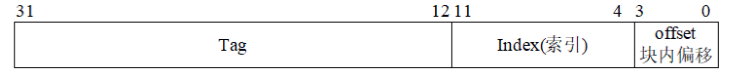
\includegraphics[width=1\linewidth]{assets/09/cache_access_address_division.png}
  \caption{Cache地址划分示意图}
  \label{fig:cache-access-address-division}
\end{figure}

\subsection{Cache模块的数据通路设计}\label{sec:09-cache-008}

\subsubsection{Cache的执行过程}\label{sec:09-cache-009}

\textbf{读操作执行过程}

\begin{itemize}
\item
  \textbf{第一拍}

  \begin{enumerate}
  \def\labelenumi{\arabic{enumi}.}
  \tightlist
  \item
    \textbf{索引值生成}：将请求中虚地址的{[}11:4{]}位作为索引值（index）送往Cache。
  \item
    \textbf{Cache行读取}：将两路Cache中对应同一index的两个Cache行都读出来。
  \item
    \textbf{地址转换}：将读操作的虚地址送往MMU逻辑进行虚实地址转换，物理地址由虚地址的组合逻辑运算结果生成。
  \item
    \textbf{地址寄存}：使用触发器（reg型变量）将物理地址寄存下来，供第二拍使用。
  \end{enumerate}
\item
  \textbf{第二拍}

  \begin{enumerate}
  \def\labelenumi{\arabic{enumi}.}
  \item
    \textbf{Tag信息比较}：

    \begin{itemize}
    \tightlist
    \item
      读取Cache RAM返回的两个Cache行的Tag信息（Cache RAM为单周期返回的同步RAM）。
    \item
      将两个Cache行的Tag信息与锁存下来的物理地址的{[}31:12{]}进行比较。
    \item
      如果某个Cache行的Tag匹配且有效位V等于1，则表示访问命中该Cache行。
    \end{itemize}
  \item
    \textbf{数据选择}：

    \begin{itemize}
    \tightlist
    \item
      根据锁存下来的虚地址的{[}3:2{]}位选择两个Cache行的Data信息，得到访问的32位数据。
    \end{itemize}
  \item
    \textbf{数据返回}：

    \begin{itemize}
    \item
      根据Tag比较结果，将命中的32位数据返回。
    \item
      如果没有命中任何Cache行，则通过总线接口向外发起访存请求，等待访存结果返回Cache模块。
    \item
      从返回结果中取出访问所在的32位数据并返回。
    \end{itemize}
  \end{enumerate}
\end{itemize}

\textbf{写操作执行过程}

\begin{itemize}
\item
  \textbf{第一拍}

  \begin{enumerate}
  \def\labelenumi{\arabic{enumi}.}
  \tightlist
  \item
    \textbf{索引值生成}：将请求中虚地址的{[}11:4{]}位作为索引值（index）送往Cache。
  \item
    \textbf{Tag信息读取}：将两路Cache中对应同一index的两个Cache行的Tag和有效位V信息读出来。
  \item
    \textbf{地址转换}：将写操作的虚地址送往MMU逻辑进行虚实地址转换，物理地址由虚地址的组合逻辑运算结果生成。
  \item
    \textbf{地址寄存}：使用触发器（reg型变量）将物理地址寄存下来，供第二拍使用。
  \end{enumerate}
\item
  \textbf{第二拍}

  \begin{enumerate}
  \def\labelenumi{\arabic{enumi}.}
  \tightlist
  \item
    \textbf{Tag信息比较}：

    \begin{itemize}
    \tightlist
    \item
      读取Cache RAM返回的两个Cache行的Tag信息（Cache RAM为单周期返回的同步RAM）。
    \item
      将两个Cache行的Tag信息与锁存下来的物理地址的{[}31:12{]}进行比较。
    \item
      如果某个Cache行的Tag匹配且有效位V等于1，则表示访问命中该Cache行。
    \end{itemize}
  \item
    \textbf{写操作准备}：

    \begin{itemize}
    \tightlist
    \item
      生成要写入的Index、路号、offset、写使能信号（写32位数据里的哪些字节）。
    \item
      将写数据传入Write Buffer。
    \end{itemize}
  \item
    \textbf{数据写入}：

    \begin{itemize}
    \tightlist
    \item
      如果Cache命中：由Write Buffer向Cache发出写请求，将Write Buffer中缓存的数据写入命中的Cache行的对应位置，并将该Cache行的脏位D置为1。
    \item
      如果Cache缺失：发起访存请求，等待访存结果返回Cache模块后，将store操作待写入的数据和访存结果拼合在一起，一并写入Cache中。
    \end{itemize}
  \end{enumerate}
\end{itemize}

\textbf{Cache缺失处理}

读、写操作都涉及Cache缺失情况下的处理，具体步骤如下：

\begin{enumerate}
\def\labelenumi{\arabic{enumi}.}
\tightlist
\item
  将Cache缺失的地址以及操作类型（如果是写操作，还要记录写数据）记录下来。
\item
  通过AXI总线接口模块向外发起对缺失Cache行的访问。访问地址是缺失Cache行的起始地址，大小是一个Cache行的大小。
\item
  在等待读请求数据返回的过程中（或同时），根据替换算法从Cache Miss地址对应index的两个Cache行中选择一个，将其整个读出。如果该Cache行的V=1且D=1，意味着这是一个有有效脏数据的Cache行，需要将该Cache行的数据通过AXI总线接口模块写出去；否则，直接丢弃该Cache行的数据。这一步还要记录选择了哪一路。
\item
  待缺失请求的数据从总线返回后，生成将要填入Cache的Cache行信息，其中Cache行的V置为1，Tag信息来自之前保存的Cache缺失的地址。如果Cache Miss请求是写操作引起的，Cache行的D置为1，Data信息是store操作待写入值部分覆盖总线返回数据后形成的新数据；否则D置为0，Data信息仅来自总线返回的数据。
\item
  将该Cache行信息填入之前记录的那个位置。
\end{enumerate}

\subsubsection{Cache表的组织管理}\label{sec:09-cache-010}

\textbf{Cache结构的表格分解}

根据Cache行中的信息，将原本的一张表拆分成多张表。对于当前实现的Cache规格，有以下表格：

\begin{itemize}
\item 两张256项×20比特的Tag表
\item 两张256项×1比特的V表
\item 两张256项×1比特的D表
\item 两张256项×128比特的Data表
\end{itemize}


每张表对应Cache的一路。Cache第i路的所有表的第i项构成第i路Cache的index=i的Cache行。所有Cache模块的操作落实到这些表上，只有读和写。下面本文将分析每张表需要支持的读写操作以及读写请求的来源。

\textbf{Cache访问类型}

依据读、写操作访问Cache执行过程中所属的不同阶段，对Cache模块进行的访问可以归纳为四种：Look Up、Hit Write、Replace和Refill。以下是这四种访问的定义：

\begin{enumerate}
\def\labelenumi{\arabic{enumi}.}
\tightlist
\item
  \textbf{Look Up}：判断是否命中Cache，并根据命中信息选取Data部分的内容。
\item
  \textbf{Hit Write}：命中的写操作进入Write Buffer，随后将数据写入命中Cache行的对应位置。
\item
  \textbf{Replace}：为了给Refill的数据腾出位置而发起的读取一个Cache行的操作。
\item
  \textbf{Refill}：将内存返回的数据（以及store miss待写入的数据）填入Replace空出的位置。
\end{enumerate}

\textbf{具体表格的读写支持}

\begin{longtable}[]{@{}
  >{\raggedright\arraybackslash}p{(\linewidth - 8\tabcolsep) * \real{0.1241}}
  >{\raggedright\arraybackslash}p{(\linewidth - 8\tabcolsep) * \real{0.1931}}
  >{\raggedright\arraybackslash}p{(\linewidth - 8\tabcolsep) * \real{0.1931}}
  >{\raggedright\arraybackslash}p{(\linewidth - 8\tabcolsep) * \real{0.1793}}
  >{\raggedright\arraybackslash}p{(\linewidth - 8\tabcolsep) * \real{0.3103}}@{}}
\toprule\noalign{}
\begin{minipage}[b]{\linewidth}\raggedright
表格类型
\end{minipage} & \begin{minipage}[b]{\linewidth}\raggedright
Look Up
\end{minipage} & \begin{minipage}[b]{\linewidth}\raggedright
Replace
\end{minipage} & \begin{minipage}[b]{\linewidth}\raggedright
Hit Write
\end{minipage} & \begin{minipage}[b]{\linewidth}\raggedright
Refill
\end{minipage} \\
\midrule\noalign{}
\endhead
\bottomrule\noalign{}
\endlastfoot
\textbf{Tag表} & 读Tag表，进行Tag比较 & 读Tag表，确定被替换行的信息 & - & 写Tag表，更新新的Tag信息 \\
\textbf{V表} (有效位表) & 读V表，判断Cache行是否有效 & 读V表，确定替换行是否有效 & - & 写V表，更新有效位 \\
\textbf{D表} (脏位表) & - & 读D表，判断被替换行是否脏 & 写D表，将命中行的脏位置为1 & 写D表，更新脏位（根据是否为写操作引起的缺失） \\
\textbf{Data表} & 读Data表，选取对应的Data部分 & 读Data表，获取被替换行的数据 & 写Data表，将数据写入命中行 & 写Data表，将新数据填入替换行 \\
\end{longtable}

对于Tag和V表，所有Cache访问的操作是一致的。因此可以将Tag表和V表横向拼接成一张\{Tag, V\}表，规格为256项×21比特，每项的{[}20:1{]}对应Tag信息，{[}0{]}对应V信息。

进一步分析，Replace和Refill不会同时发生，这意味着对所有表格，Replace的读和Refill的写不会同时进行。由于设计的是阻塞式Cache，在进行Replace和Refill操作时不接收新的访问请求，也不会有Cache命中的store操作。因此，Replace和Refill的读写操作不会与Look Up和Hit Write的读写操作同时发生。此外，Hit Write不访问\{Tag, V\}表，因此\{Tag, V\}表同一时刻至多接收一个读请求或写请求；Look Up不访问D表，因此D表同一时刻至多接收一个读请求或写请求。

Data表的情况较复杂，因为Look Up和Hit Write可能同时发生。直接方案是让Data表支持同时读写，但这种设计成本较高。另一方案是阻塞读操作的Look Up，以避免与Hit Write冲突，虽然降低电路开销但牺牲性能。更好的方法是将Data表横向拆分成四个Bank表，每个规格为256项×32比特。这样，当Look Up和Hit Write不冲突时，可以同时进行；如有冲突，则阻塞Look Up。此方法性能损失较少，且Bank表的写粒度需精细到字节，以支持SB、SH等写操作。

根据以上分析，Cache最终需要使用的存储器规格如下：

\begin{longtable}[]{@{}
  >{\raggedright\arraybackslash}p{(\linewidth - 8\tabcolsep) * \real{0.1733}}
  >{\raggedright\arraybackslash}p{(\linewidth - 8\tabcolsep) * \real{0.1600}}
  >{\raggedright\arraybackslash}p{(\linewidth - 8\tabcolsep) * \real{0.1200}}
  >{\raggedright\arraybackslash}p{(\linewidth - 8\tabcolsep) * \real{0.1333}}
  >{\raggedright\arraybackslash}p{(\linewidth - 8\tabcolsep) * \real{0.4133}}@{}}
\toprule\noalign{}
\begin{minipage}[b]{\linewidth}\raggedright
表格名称
\end{minipage} & \begin{minipage}[b]{\linewidth}\raggedright
规格
\end{minipage} & \begin{minipage}[b]{\linewidth}\raggedright
实现方式
\end{minipage} & \begin{minipage}[b]{\linewidth}\raggedright
实例化数量
\end{minipage} & \begin{minipage}[b]{\linewidth}\raggedright
备注
\end{minipage} \\
\midrule\noalign{}
\endhead
\bottomrule\noalign{}
\endlastfoot
\{Tag, V\}表 & 256项×21比特 & Block RAM & 2 & 每项{[}20:1{]}为Tag信息，{[}0{]}为V信息 \\
Data Bank表 & 256项×32比特 & Block RAM & 8 & 支持字节写使能 \\
D表（脏位表） & 256项×1比特 & Regfile & 2 & - \\
\end{longtable}

\subsection{Cache模块功能边界划分}\label{sec:09-cache-011}

\subsubsection{Cache与CPU的交互}\label{sec:09-cache-012}

基于当前的设计要求，我们希望在Cache与CPU流水线之间的功能边界划分上与现有的``类SRAM-AXI''转接桥和CPU流水线之间的功能边界划分保持一致。具体而言，即是由CPU流水线向Cache模块发送请求，而Cache模块则负责向CPU流水线返回数据或确认写入成功的响应。这样划分后，CPU流水线部分基本无需进行改动。

由于我们采用VIPT（Virtually Indexed Physically Tagged）方式进行Cache访问，因此需要CPU中的TLB（Translation Lookaside Buffer）模块将转换后的物理地址传送至Cache模块。Cache模块接收该物理地址并将其寄存一个时钟周期，然后使用该物理地址进行Cache Tag比较。

总结如下：

\begin{enumerate}
\item \textbf{功能边界划分}：
\begin{itemize}
\item CPU流水线发送请求至Cache模块。
\item Cache模块返回数据或写成功响应至CPU流水线。
\end{itemize}
\end{enumerate}


\begin{enumerate}
\def\labelenumi{\arabic{enumi}.}
\setcounter{enumi}{1}
\tightlist
\item
  \textbf{VIPT Cache访问}：

  \begin{itemize}
  \tightlist
  \item
    TLB模块在CPU中进行虚拟地址到物理地址的转换。
  \item
    转换后的物理地址传送至Cache模块。
  \item
    Cache模块将物理地址寄存一个时钟周期用于Tag比较。
  \end{itemize}
\end{enumerate}

以下是一个可能的Cache模块与CPU流水线的交互接口定义：

\begin{longtable}[]{@{}
  >{\raggedright\arraybackslash}p{(\linewidth - 6\tabcolsep) * \real{0.0933}}
  >{\raggedright\arraybackslash}p{(\linewidth - 6\tabcolsep) * \real{0.0533}}
  >{\raggedright\arraybackslash}p{(\linewidth - 6\tabcolsep) * \real{0.0533}}
  >{\raggedright\arraybackslash}p{(\linewidth - 6\tabcolsep) * \real{0.8000}}@{}}
\toprule\noalign{}
\begin{minipage}[b]{\linewidth}\raggedright
名称
\end{minipage} & \begin{minipage}[b]{\linewidth}\raggedright
位宽
\end{minipage} & \begin{minipage}[b]{\linewidth}\raggedright
方向
\end{minipage} & \begin{minipage}[b]{\linewidth}\raggedright
含义
\end{minipage} \\
\midrule\noalign{}
\endhead
\bottomrule\noalign{}
\endlastfoot
valid & 1 & IN & 表明请求有效 \\
op & 1 & IN & 1：WRITE；0：READ \\
index & 8 & IN & 地址的index域(addr{[}11:4{]}) \\
tag & 20 & IN & 经虚实地址转换后的paddr形成的tag，由于来自组合逻辑运算，故与index是同拍信号。 \\
offset & 4 & IN & 地址的offset域(addr{[}3:0{]}) \\
wstrb & 4 & IN & 写字节使能信号 \\
wdata & 32 & IN & 写数据 \\
addr\_ok & 1 & OUT & 该次请求的地址传输OK，读：地址被接收；写：地址和数据被接收 \\
data\_ok & 1 & OUT & 该次请求的数据传输OK，读：数据返回；写：数据写入完成 \\
rdata & 32 & OUT & 读Cache的结果 \\
\end{longtable}

\subsubsection{Cache与AXI总线的交互}\label{sec:09-cache-013}

为了更好地划分Cache模块通过AXI总线接口访存的功能，需要详细考虑各个功能模块的分工和接口设计。最直接的方式是将所有功能都集中到Cache模块中，实际上将现有的``类SRAM-AXI''转接桥整体替换为新的Cache模块。然而，考虑到Cache模块中包含大量AXI协议处理的逻辑，这种设计显然不够合理，即使将其命名为cache\_mem\_module，模块内部的功能仍然过于复杂。因此，本文建议保留一个内部访存总线到AXI总线的接口转换模块。

该接口转换模块对CPU内部提供多个端口，而对CPU外部仅暴露一个AXI总线接口。通过这种设计，多个请求的仲裁以及AXI协议的处理都集中在这个模块中，使得Cache模块与AXI总线接口模块之间的功能划分更加简洁清晰。Cache模块仅向AXI总线接口模块发送访存请求，AXI总线接口模块则负责返回数据或响应信号。

基于上述划分，Cache模块向AXI总线接口模块发送的请求包含地址、操作类型、长度等信息，这些信息量较小，可以在一个时钟周期内完成交互。然而，需要重点考虑的是读写数据的交互方式。由于Cache行大小为16字节，我们希望在AXI总线上采用突发（Burst）访问模式，以最大限度减少请求通道上的交互开销。这样，问题的关键在于Cache模块和AXI总线接口模块之间的数据交互是否也需要定义类似的Burst传输模式，或者两者在一个时钟周期内完成16字节数据的交互。

设计的关键点在于我们设计目标的优先级。对于本书的学习目标，首先是确保功能的实现，其次是保证性能达标，最后才是功耗优化。在此背景下，我们的设计建议如下：

\begin{enumerate}
\def\labelenumi{\arabic{enumi}.}
\tightlist
\item
  \textbf{读操作}：AXI总线接口模块每个周期最多向Cache模块返回32位数据。Cache模块将返回的数据填入Cache的Bank RAM中或直接返回给CPU流水线。
\item
  \textbf{写操作}：Cache模块在一个周期内直接将一个Cache行的数据传输给AXI总线接口模块。AXI总线接口模块内部设置一个16字节的写缓存来存储这些数据，然后再以突发方式逐步发出。
\end{enumerate}

下表是一个可能的接口设计方案：

\begin{longtable}[]{@{}
  >{\raggedright\arraybackslash}p{(\linewidth - 6\tabcolsep) * \real{0.1169}}
  >{\raggedright\arraybackslash}p{(\linewidth - 6\tabcolsep) * \real{0.0519}}
  >{\raggedright\arraybackslash}p{(\linewidth - 6\tabcolsep) * \real{0.0519}}
  >{\raggedright\arraybackslash}p{(\linewidth - 6\tabcolsep) * \real{0.7792}}@{}}
\toprule\noalign{}
\begin{minipage}[b]{\linewidth}\raggedright
名称
\end{minipage} & \begin{minipage}[b]{\linewidth}\raggedright
位宽
\end{minipage} & \begin{minipage}[b]{\linewidth}\raggedright
方向
\end{minipage} & \begin{minipage}[b]{\linewidth}\raggedright
含义
\end{minipage} \\
\midrule\noalign{}
\endhead
\bottomrule\noalign{}
\endlastfoot
rd\_req & 1 & OUT & 读请求有效信号。高电平有效。 \\
rd\_type & 3 & OUT & 读请求类型。3'b000------字节，3'b001------半字，3'b010------字，3'b100------Cache行。 \\
rd\_addr & 32 & OUT & 读请求起始地址。 \\
rd\_rdy & 1 & IN & 读请求能否被接收的握手信号。高电平有效。 \\
ret\_valid & 1 & IN & 返回数据有效信号。高电平有效。 \\
ret\_last & 2 & IN & 返回数据是一次读请求对应的最后一个返回数据。 \\
ret\_data & 32 & IN & 读返回数据。 \\
wr\_req & 1 & OUT & 写请求有效信号。高电平有效。 \\
wr\_type & 3 & OUT & 写请求类型。3'b000------字节，3'b001------半字，3'b010------字，3'b100------Cache行。 \\
wr\_addr & 32 & OUT & 写请求起始地址。 \\
wr\_wstrb & 4 & OUT & 写操作的字节掩码。仅在写请求类型为3'b000、3'b001、3'b010情况下才有意义。 \\
wr\_data & 128 & OUT & 写数据。 \\
wr\_rdy & 1 & IN & 写请求能否被接收的握手信号。高电平有效。此处要求wr\_rdy要先于wr\_req置起，wr\_req看到wr\_rdy后才可能置上。所以wr\_rdy的生成不要组合逻辑依赖wr\_req，它应该是当AXI总线接口内部的16字节写缓存为空时就置上。 \\
\end{longtable}

\subsection{Cache模块内除Cache表之外的数据通路}\label{sec:09-cache-014}

本文介绍的是阻塞式Cache，Look Up与Replace \& Refill可以共享部分数据通路。其核心组件包括Request Buffer、Tag Compare、Data Select、Miss Buffer和LFSR。Hit Write是独立于Look Up和Replace \& Refill之外的操作，其核心组件是Write Buffer。

\textbf{Request Buffer}

Request Buffer的主要功能是锁存操作请求信息，包括op、index、tag、offset、wstrb、wdata等。由于RAM读操作会跨越两个时钟周期，因此Request Buffer的输出与RAM读出的Tag和Data信息处于同一时钟周期。在阻塞式Cache设计中，Request Buffer不仅维护Tag比较时需要的信息，还维护Miss处理时所需的信息。

\textbf{Tag Compare}

Tag Compare模块的功能是将每一路Cache中读出的Tag与Request Buffer中寄存的tag（记为reg\_tag）进行比较，生成命中结果（此处不考虑Uncache情况，对于Uncache，必须不命中）。其Verilog代码示例如下：

% 代码语言：BookVerilog
\begin{CodeBlock}[language=BookVerilog]
assign way0_hit = way0_v && (way0_tag == reg_tag);
assign way1_hit = way1_v && (way1_tag == reg_tag);
assign cache_hit = way0_hit || way1_hit;
\end{CodeBlock}

\textbf{Data Select}

Data Select模块的功能是从两路Cache中读出的Data信息中选择合适的数据，生成访问操作的结果。对于命中的Load操作，首先用地址的{[}3:2{]}从每一路Cache读出的Data数据中选择一个字，然后根据Cache命中的结果从两个字中选择出Load的结果（此处不考虑Miss情况，若Miss，Load的最终结果来自AXI接口的返回，因此这里应该是一个三选一逻辑）。对于Replace操作，只需要根据替换算法决定的路信息，将读出的Data选择出来即可。其Verilog代码示例如下：

% 代码语言：BookVerilog
\begin{CodeBlock}[language=BookVerilog]
assign way0_load_word = way0_data[pa[3:2]*32 +: 32];
assign way1_load_word = way1_data[pa[3:2]*32 +: 32];
assign load_res = ({32{way0_hit}} & way0_load_word) | ({32{way1_hit}} & way1_load_word); 
// 若考虑miss，应该是三选一

assign replace_data = replace_way ? way1_data : way0_data;
\end{CodeBlock}

\textbf{Miss Buffer}

Miss Buffer用于记录缺失Cache行准备替换的路信息，以及已经从AXI总线返回的32位数据数量。Miss处理所需的地址、是否是Store指令等信息依然由Request Buffer维护。

\textbf{LFSR}

LFSR（线性反馈移位寄存器）用于实现伪随机替换算法，作为伪随机数源。

\textbf{Write Buffer}

Write Buffer在Hit Write（Store操作在Look Up时发现命中Cache）时启动，它寄存Store要写入的way、bank、index、bank内字节写使能和写数据，然后使用寄存后的值写入Cache。

\subsection{Cache模块内部的控制逻辑设计}\label{sec:09-cache-015}

\subsubsection{Cache模块自身的状态机设计}\label{sec:09-cache-016}

为应对操作可能发生的Cache Miss情况，在发生Cache Miss后，需要向AXI总线发出读请求并对Cache RAM进行替换和重填充操作。为了有效控制这一系列操作，我们引入了一套状态机机制。由于我们实现的是阻塞式Cache，在Cache Miss时不会接收新的请求，因此Look Up和Replace \& Refill处理可以共用一个状态机（称为主状态机）。此外，Hit Write是独立于Look Up和Replace \& Refill之外的单独访问，我们用一个单独的状态机进行维护，称之为Write Buffer状态机。

主状态机包括以下五个状态，如图\ref{fig:cache-fsm}a所示 ：

\begin{enumerate}
\def\labelenumi{\arabic{enumi}.}
\tightlist
\item
  \textbf{IDLE}：Cache模块当前没有任何操作。
\item
  \textbf{LOOKUP}：Cache模块正在执行一个操作并且得到了查询结果。
\item
  \textbf{MISS}：Cache模块当前处理的操作发生Cache Miss，正在等待AXI总线的wr\_rdy信号。
\item
  \textbf{REPLACE}：待替换的Cache行已经从Cache中读出，正在等待AXI总线的rd\_rdy信号。
\item
  \textbf{REFILL}：Cache缺失的访存请求已发出，准备/正在将缺失的Cache行数据写入Cache中。
\end{enumerate}

\begin{figure}[htbp]
  \centering
  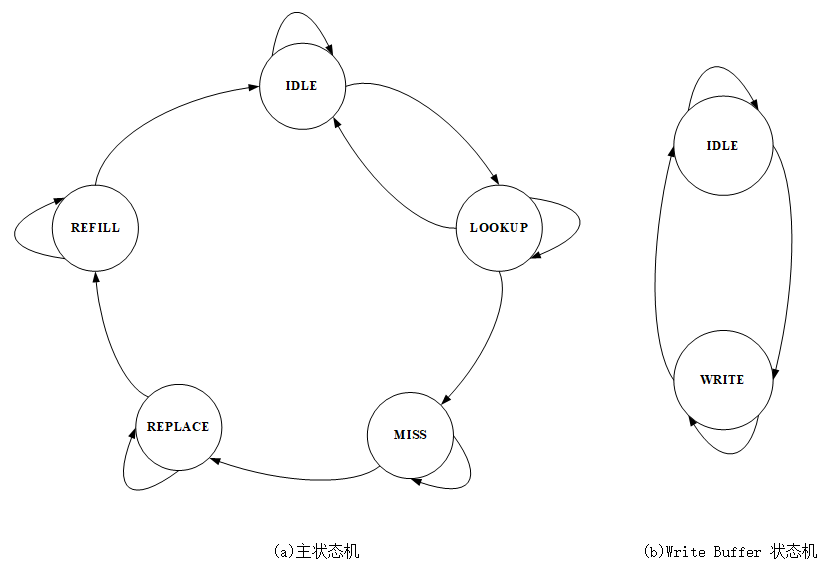
\includegraphics[width=1\linewidth]{assets/09/cache_fsm.png}
  \caption{Cache模块主状态机状态转移图}
  \label{fig:cache-fsm}
\end{figure}

Write Buffer状态机共包括2个状态，见图\ref{fig:cache-fsm}b。

\begin{itemize}
\tightlist
\item
  \textbf{IDLE}：Write Buffer当前没有待写的数据。
\item
  \textbf{WRITE}：将待写数据写入到Cache中。在主状态机处于LOOKUP状态且发现Store操作命中Cache时，触发Write Buffer状态机进入WRITE状态，同时Write Buffer会寄存Store要写入的Index、路号、offset、写使能（写32位数据里的哪些字节）和写数据。
\end{itemize}

以下是主状态机各状态之间的转换条件的详细说明：

\begin{enumerate}
\def\labelenumi{\arabic{enumi}.}
\tightlist
\item
  \textbf{IDLE}：

  \begin{itemize}
  \tightlist
  \item
    \textbf{IDLE → IDLE}：在这一时钟周期内，流水线没有新的Cache访问请求，或者有请求但因与Hit Write冲突而无法被Cache接收。
  \item
    \textbf{IDLE → LOOKUP}：在这一时钟周期内，Cache接收到了流水线发来的一个新的Cache访问请求（必定与Hit Write无冲突）。
  \end{itemize}
\item
  \textbf{LOOKUP}：

  \begin{itemize}
  \tightlist
  \item
    \textbf{LOOKUP → IDLE}：当前处理的操作是Cache命中，且在这一时钟周期内流水线没有新的Cache访问请求，或者有请求但因与Hit Write冲突而无法被Cache接收。
  \item
    \textbf{LOOKUP → LOOKUP}：当前处理的操作是Cache命中，且在这一时钟周期内Cache接收到了流水线发来的一个新的Cache访问请求（必定与Hit Write无冲突）。
  \item
    \textbf{LOOKUP → MISS}：当前处理的操作是Cache缺失。
  \end{itemize}
\item
  \textbf{MISS}：

  \begin{itemize}
  \tightlist
  \item
    \textbf{MISS → MISS}：AXI总线接口模块反馈wr\_rdy为0（注意，wr\_rdy应当先于wr\_req置上）。
  \item
    \textbf{MISS → REPLACE}：AXI总线接口模块反馈wr\_rdy为1（表示AXI总线内部16字节写缓存为空，可以接收wr\_req）。当wr\_rdy为1时，对Cache发起替换的读请求，并转到REPLACE状态。
  \end{itemize}
\item
  \textbf{REPLACE}：

  \begin{itemize}
  \tightlist
  \item
    \textbf{REPLACE → REPLACE}：AXI总线接口模块反馈rd\_rdy为0。刚进入REPLACE的第一时钟周期，会得到被替换的Cache行数据，并发起wr\_req送到AXI总线接口。由于wr\_rdy为1，故wr\_req一定会被接收。同时，对AXI总线发起缺失Cache的读请求。
  \item
    \textbf{REPLACE → REFILL}：AXI总线接口模块反馈rd\_rdy为1，表示对AXI总线发起的缺失Cache的读请求将被接收。
  \end{itemize}
\item
  \textbf{REFILL}：

  \begin{itemize}
  \tightlist
  \item
    \textbf{REFILL → REFILL}：缺失Cache行的最后一个32位数据（ret\_valid=1 \&\& ret\_last=1）尚未返回。
  \item
    \textbf{REFILL → IDLE}：缺失Cache行的最后一个32位数据（ret\_valid=1 \&\& ret\_last=1）从AXI总线接口模块返回。
  \end{itemize}
\end{enumerate}

以下是Write Buffer状态机各状态之间的转换条件的详细说明：

\begin{enumerate}
\def\labelenumi{\arabic{enumi}.}
\tightlist
\item
  \textbf{IDLE}：

  \begin{itemize}
  \tightlist
  \item
    \textbf{IDLE → IDLE}：在这一时钟周期内，Write Buffer没有待写的数据，并且主状态机没有新的Hit Write。
  \item
    \textbf{IDLE → WRITE}：在这一时钟周期内，Write Buffer没有待写的数据，并且主状态机发现新的Hit Write（主状态机处于LOOKUP状态且发现Store操作命中Cache）。
  \end{itemize}
\item
  \textbf{WRITE}：

  \begin{itemize}
  \tightlist
  \item
    \textbf{WRITE → WRITE}：在这一时钟周期内，Write Buffer有待写的数据，并且主状态机发现新的Hit Write。
  \item
    \textbf{WRITE → IDLE}：在这一时钟周期内，Write Buffer有待写的数据，并且主状态机没有新的Hit Write。
  \end{itemize}
\end{enumerate}

在主状态机的状态转换过程中，多次提到``与Hit Write有/无冲突''，这里的冲突分为两种情况：

\begin{enumerate}
\def\labelenumi{\arabic{enumi}.}
\item
  \textbf{主状态机处于LOOKUP状态且发现Store操作命中Cache}：此时，如果流水线发来一个新的Load类的Cache访问请求，并且该Load请求与LOOKUP状态的Store请求地址存在写后读相关性，即产生``与Hit Write冲突''。
\item
  \textbf{Write Buffer状态机处于WRITE状态}：即正在将待写数据写入Cache中，如果此时流水线发来一个新的Load类的Cache访问请求，并且该Load请求与Write Buffer中的待写请求的地址重叠。这里的``地址重叠''指的是Load请求地址的{[}3:2{]}与Store请求地址的{[}3:2{]}相等。
\end{enumerate}

以上两种情况都视为``与Hit Write冲突''。尽管对于第一种情况，可以采用``Write Buffer前递给LOOKUP''的方法解决，而不阻塞主状态机的转换，但为了简化，我们推荐采用阻塞方式处理。然而，第二种情况只能通过阻塞方式解决，即阻塞主状态机的转换。这种方法牺牲了一定的性能，但简化了设计。

在主状态机``LOOKUP → LOOKUP''的转换中，应注意避免引入RAM输出端到RAM输入端的路径。具体而言，主状态机发现一个命中的Cache访问并接收到一个新的Cache访问请求时，应避免使用命中信息（来自RAM读出的Tag比较）控制新的RAM的读使能。我们的解决方案是，无论LOOKUP状态的请求是否命中Cache，在控制``Hit Write冲突''和新的RAM使能生成时都视为命中考虑。即使最终发现不命中，也不会导致错误。

在主状态机``MISS → REPLACE''的转换过程中，当处于MISS状态时，我们确保AXI总线接口可以接收被替换Cache行的数据，同时对Cache RAM发起替换Cache行的读请求。下一拍（REPLACE状态）中，获得被替换的Cache行数据并将其发送到AXI总线接口模块（此时一定可以被接收）。同时，我们可以对AXI总线发起缺失Cache行的读请求。这种设计通过牺牲一定的性能来降低Cache模块和AXI总线接口模块在读返回路径上的握手复杂性，实现了无条件地将总线接口模块返回的数据直接写入Cache中。

需要提醒的是，对于ICache，可以将wr\_rdy恒设为1（此时MISS状态只会持续一拍），因为ICache不会真正发出wr\_req。

\subsubsection{表的片选和写使能}\label{sec:09-cache-017}

下表展示了Cache片选和写使能的逻辑：

\begin{longtable}[]{@{}
  >{\raggedright\arraybackslash}p{(\linewidth - 10\tabcolsep) * \real{0.0818}}
  >{\raggedright\arraybackslash}p{(\linewidth - 10\tabcolsep) * \real{0.0545}}
  >{\raggedright\arraybackslash}p{(\linewidth - 10\tabcolsep) * \real{0.1545}}
  >{\raggedright\arraybackslash}p{(\linewidth - 10\tabcolsep) * \real{0.3455}}
  >{\raggedright\arraybackslash}p{(\linewidth - 10\tabcolsep) * \real{0.1818}}
  >{\raggedright\arraybackslash}p{(\linewidth - 10\tabcolsep) * \real{0.1818}}@{}}
\toprule\noalign{}
\begin{minipage}[b]{\linewidth}\raggedright
Cache表项
\end{minipage} & \begin{minipage}[b]{\linewidth}\raggedright
\end{minipage} & \begin{minipage}[b]{\linewidth}\raggedright
Look Up
\end{minipage} & \begin{minipage}[b]{\linewidth}\raggedright
Hit Write
\end{minipage} & \begin{minipage}[b]{\linewidth}\raggedright
Replace
\end{minipage} & \begin{minipage}[b]{\linewidth}\raggedright
Refill
\end{minipage} \\
\midrule\noalign{}
\endhead
\bottomrule\noalign{}
\endlastfoot
\{Tag，V\} & 片选 & 2路 & - & & 替换那一路 \\
& 写使能 & 2路 & - & & 替换那一路 \\
D & 片选 & - & Write Buffer记录的那一路 & 替换那一路 & 替换那一路 \\
& 写使能 & - & Write Buffer记录的那一路 & - & 替换那一路 \\
Data & 片选 & 2路，请求所在Bank & Write Buffer记录的那一路，请求所在Bank & 替换那一路，所有Bank & 替换那一路，所有Bank \\
& 写使能 & - & Write Buffer记录的那一路，请求所在Bank & - & 替换那一路，所有Bank \\
\end{longtable}

\subsubsection{模块接口输出的控制相关信号}\label{sec:09-cache-018}

以下是对模块接口输出的控制相关信号置1条件的分析：

\textbf{流水线方向的 \texttt{addr\_ok} 信号}

\begin{itemize}
\tightlist
\item
  Cache主状态机处于 \texttt{IDLE} 状态。
\item
  或者，Cache主状态机处于 \texttt{LOOKUP} 状态，并将进行 \texttt{LOOKUP\ →\ LOOKUP} 的转换，具体包括：

  \begin{itemize}
  \tightlist
  \item
    \texttt{LOOKUP} 发现Cache命中，流水线发送来的新的Cache请求是写操作；
  \item
    \texttt{LOOKUP} 发现Cache命中，且新的Cache请求是读操作且无``Hit Write冲突''。
  \end{itemize}
\end{itemize}

\textbf{流水线方向的 \texttt{data\_ok} 信号}

\begin{itemize}
\tightlist
\item
  Cache当前状态为 \texttt{LOOKUP} 且Cache命中。
\item
  或者，Cache当前状态为 \texttt{LOOKUP} 且处理的是写操作。
\item
  或者，Cache当前状态为 \texttt{REFILL} 且 \texttt{ret\_valid=1}，同时Miss Buffer中记录的返回字个数与Cache缺失地址的 \texttt{{[}3:2{]}} 相等。
\end{itemize}

\textbf{AXI接口方向的 \texttt{rd\_req} 信号}

\begin{itemize}
\tightlist
\item
  当Cache模块状态机处于 \texttt{REPLACE} 状态时，组合逻辑将 \texttt{rd\_req} 置为1。在非 \texttt{REPLACE} 状态时，\texttt{rd\_req} 自然为0。
\end{itemize}

\textbf{AXI接口方向的 \texttt{wr\_req} 信号}

\begin{itemize}
\tightlist
\item
  设置一个触发器，复位期间清0。当Cache模块状态机从 \texttt{MISS} 转换到 \texttt{REPLACE} 状态时，将其置1。随后，当 \texttt{wr\_rdy} 为1时，将其从1清为0。
\end{itemize}

\subsection{Cache的硬件初始化问题}\label{sec:09-cache-019}

在LoongArch精简版指令集中，Cache可以通过软件进行初始化。在处理器复位结束后，CSR.CRMD的DATF和DMTM域都为0，此时取指和访存都是强序非缓存的，软件可以使用CACOP指令将Cache的Tag部分置为0。

在我们的实践工作中，考虑到实现工作量和理解上的复杂度，一般的我们将CACHE指令的实现放在了Cache实现的最后一个阶段。这引发了一个问题：在尚未实现CACOP指令的情况下，如何在上板验证时确保Cache已初始化。

Cache初始化至少要确保Cache中每一项的Tag、V和D的状态置为确定的无效值。由于Tag和V信息都存放在RAM中，因此解决方案是设计一个小型硬件电路，将存放Cache Tag和V信息的RAM的每一行写成全0值。还有一个偷懒的方法：利用实验中采用FPGA 硬件平台这一特点来简化Cache硬件初始化的实现。读者可以在生成Cache所用的RAM的时候，选择将RAM初始化成全0。

\section{Cache性能分析与优化}\label{sec:09-cache-020}

\textbf{Cache性能分析关键指标}

\begin{enumerate}
\def\labelenumi{\arabic{enumi}.}
\item
  \textbf{命中时的访问延迟（Hit Latency）}：命中时的访问延迟是指当Cache命中时，从发出请求到数据返回所需的时间。这一指标通常反映了Cache访问速度的快慢。理想情况下，命中时的访问延迟应该尽可能低，以确保快速的数据访问。
\item
  \textbf{失效时的访问延迟（Miss Latency）}：失效时的访问延迟是指当Cache未命中（Cache Miss）时，从发出请求到数据返回所需的时间。这一时间包括从主存储器或下一级Cache中获取数据并将其载入Cache的过程。失效时的访问延迟通常比命中时的访问延迟要高得多，因为涉及到更长的路径和更高的访问成本。
\item
  \textbf{失效时对后续访问的影响（Miss Penalty）}：失效时对后续访问的影响是指一次Cache失效对后续访问造成的额外延迟。这不仅包括获取所需数据的时间，还可能包括在载入新数据时将旧数据写回主存储器的时间。高失效率会导致频繁的Cache Miss，从而显著降低系统的整体性能。
\end{enumerate}

\textbf{可能的优化方向}

\begin{enumerate}
\def\labelenumi{\arabic{enumi}.}
\item
  \textbf{增大Cache容量}
  增大Cache容量可以减少Cache Miss的发生几率，从而降低失效时的访问延迟和对后续访问的影响。然而，增大容量也会增加Cache的物理尺寸和成本，并可能导致访问延迟增加。
\item
  \textbf{提高Cache的相联度}
  提高Cache的相联度（Associativity）可以减少冲突Miss的发生。全相联Cache的性能最好，但实现复杂度和成本较高。可以采用较高相联度的组相联Cache作为折中方案。
\item
  \textbf{采用多级Cache架构}
  现代处理器通常采用多级Cache（L1、L2、L3等）架构。较小的L1 Cache提供低延迟访问，而较大的L2、L3 Cache提供更大的存储容量。多级Cache架构可以在不同层次上优化访问延迟和Miss率。
\item
  \textbf{使用预取（Prefetching）技术}
  预取技术通过在实际访问前提前加载数据到Cache中来减少Miss率。预取可以是硬件预取或软件预取，但需要平衡预取的准确性和额外的带宽消耗。
\item
  \textbf{优化Cache替换算法}
  采用更智能的替换算法（如LRU、LFU等）可以减少不必要的数据替换，提高命中率。替换算法的选择对Cache性能有重要影响。
\item
  \textbf{减少Cache一致性开销}
  在多核处理器中，Cache一致性协议（如MESI、MOESI）用于确保各核Cache中的数据一致性。优化一致性协议或减少一致性开销可以提高Cache性能。
\end{enumerate}

\section{Cache集成到CPU中}\label{sec:09-cache-021}

事实上这部分内容在\textbf{Cache模块功能边界划分}部分已经给出了实现方案，按照接口定义将Cache对接进流水线即可。为避免读者陷入工程细节，本条主要在宏观层面上给出整体的实现思路

\textbf{命中情况下的适配}

当Cache命中时，数据可以在一个时钟周期内从Cache中获取（尽管一个完整的访存过程会经历两个以上周期，但是流水线技术有效的掩盖了这个问题，即整体看来，访存流水线每周期可处理一条访存指令），这对于流水线来说是理想的情况。在经典的五级RISC流水线中（取指、译码、执行、存储访问、写回），Cache命中意味着存储访问阶段（MEM）能够在一个周期内完成，从而不影响流水线的顺利进行。这样可以保持流水线的高效运行，减少等待时间和潜在的流水线停顿。

\textbf{缺失情况下的适配}

当Cache缺失（Cache Miss）时，CPU流水线必须等待从主存或更低级的存储器获取数据，这会导致流水线停顿。具体而言，缺失会触发一个存储访问异常，Cache一般使用状态机处理数据缺失，需要多个周期来完成数据的读取。这种情况，顺序执行的处理器通常会暂停流水线以保持流水线同步，但这也意味着处理器效率下降。为了应对这一问题，现代处理器通常会使用非阻塞缓存（Non-blocking Cache）和乱序执行（Out-of-order Execution）来减少Cache Miss对流水线的影响。

\textbf{Uncache访问的处理}

Uncache访问（非缓存访问）通常用于访问那些不适合缓存的数据，比如I/O设备的寄存器。这类访问直接与主存或I/O设备交互，不经过Cache，因此延迟较高。为了适应这类访问，CPU通常设计专门的路径和控制逻辑，以确保数据的正确性和一致性。当然为了方便实现也可以复用Cache的访存状态机，即强制让Uncache访问指令发生Cache缺失，从而启动Cache的恢复流程，利用Cache在该流程中的写回和读取逻辑完成Uncache访问功能。

\section{支持Cache处理器的性能调优}\label{sec:09-cache-022}

在确定架构完成Cache的集成后，在最顶层宏观的方法学视角上处理器已经没有较大的优化空间了。但在具体的实践中，即使不改变整体架构，处理器的性能往往还有较大的提升空间，这主要是因为我们实现的处理器很可能存在``性能BUG''。\textbf{解决这些性能BUG的过程就是性能调优的过程。}

在面对复杂系统的性能优化时，我们经常需要做出许多决策，例如确定哪些部分值得优化、选择哪种优化策略、预测可能的收益以及评估这些策略的成本。显然，如果巨大的努力仅带来微小的性能提升，这并不符合我们的预期。因此，相较于盲目编程，我们更需要一套科学的方法论来指导我们解答以下关键问题：

\begin{enumerate}
\def\labelenumi{\arabic{enumi}.}
\tightlist
\item
  \textbf{评估当前性能}：通过定量的指标，如执行时间和资源利用率，来全面了解系统的现状。
\item
  \textbf{识别性能瓶颈}：通过性能分析工具，如性能分析器和日志分析，来确定影响系统效率的关键因素。
\item
  \textbf{选择适当的优化策略}：根据瓶颈的性质，决定采取算法优化、资源增配、系统配置调整等方法。
\item
  \textbf{评估优化效果}：实施优化后，再次进行性能评估，并与优化前的性能数据进行对比，以验证优化的有效性是否符合预期。
\end{enumerate}

\subsection{性能评估}\label{sec:09-cache-023}

在讨论性能优化之前，首先必须确立系统当前的运行状态。因此，我们需要一个定量的性能衡量指标，而不仅仅依赖主观感觉来判断系统的运行效果。通过这种定量指标，我们能够客观评估现有系统的性能，这是性能优化的初步步骤。

在通常的理解中，``高性能''往往意味着``运行速度快''。因此，一个直观的性能衡量指标是程序的执行时间。简而言之，评估一个系统的性能就是测量程序在该系统上的执行时间。通过这种方法，我们可以准确地识别出性能瓶颈，从而有针对性地进行优化。

在选择基准程序时，关键在于选取能够代表实际应用场景的程序集。这些程序应当能够反映出在特定优化技术下，预期性能提升与实际应用场景中性能提升的一致趋势。

\subsubsection{基准测试程序}\label{sec:09-cache-024}

不同的应用场景可能需要不同的代表性程序，从而形成各自的benchmark。例如，Linpack被用于代表超级计算场景，MLPerf针对的是机器学习训练场景，CloudSuite用于云计算场景，而Embench则专注于嵌入式场景。对于通用计算场景，最著名的benchmark是SPEC CPU，由Standard Performance Evaluation Corporation (SPEC) 组织发布，该组织旨在建立和维护用于评估计算机系统性能的标准。

SPEC CPU 2006是一个广泛使用的benchmark，包括整数和浮点测试，涵盖了多种应用程序，例如：

\begin{itemize}
\tightlist
\item
  \textbf{整数测试}：

  \begin{itemize}
  \tightlist
  \item
    \texttt{400.perlbench}：利用Perl语言检测垃圾邮件
  \item
    \texttt{401.bzip2}：bzip压缩算法
  \item
    \texttt{403.gcc}：gcc编译器
  \item
    \texttt{429.mcf}：针对大型公共交通中单站车辆调度的组合优化问题
  \item
    \texttt{445.gobmk}：围棋AI搜索问题
  \item
    \texttt{456.hmmer}：使用隐马尔可夫模型进行基因序列搜索
  \item
    \texttt{458.sjeng}：国际象棋AI搜索问题
  \item
    \texttt{462.libquantum}：量子计算模拟素数分解
  \item
    \texttt{464.h264ref}：对YUV格式源文件进行H.264视频编码
  \item
    \texttt{471.omnetpp}：大型CSMA/CD协议以太网模拟
  \item
    \texttt{473.astar}：使用A*算法进行路径寻找
  \item
    \texttt{483.xalancbmk}：XML到HTML的格式转换
  \end{itemize}
\item
  \textbf{浮点测试}：

  \begin{itemize}
  \tightlist
  \item
    覆盖流体力学、量子化学、生物分子研究、有限元分析、线性规划、影像光线追踪、计算电磁学、天气预报、语音识别等领域。
  \end{itemize}
\end{itemize}

随着技术的演进，benchmark也需要不断更新以反映新的应用趋势。例如，SPEC CPU 2017版本引入了一些新程序，如生物医学成像、3D渲染和动画、采用蒙特卡罗树搜索的人工智能围棋程序，这些新加入的测试项目大大提高了benchmark的时代相关性和实用性。通过这些更新，SPEC帮助研究人员和工程师准确评估和优化不断变化的技术环境中的系统性能。

但对于面向教学的CPU设计实践来说, SPEC CPU的程序有点过于真实了: 一方面它们的规模很大, 即使在x86真机中也需要花费小时的时间来运行; 另一方面它们需要运行在Linux环境中, 这意味着我们首先需要设计一个能正确启动Linux的CPU, 然后才能运行SPEC CPU这个benchmark。对于我们的应用场景来说，传统的Dhrystone与CoreMark测试程序已经足够了。

\textbf{Dhrystone}

Dhrystone是一种经典的CPU性能基准测试程序，主要用于评估整数运算的性能。它以其简单、便于移植和使用广泛而著称。Dhrystone使用合成的程序来模拟常见的计算工作负载，通过测量在特定时间内执行的Dhrystone操作数（DMIPS），来评估CPU的性能。然而，Dhrystone的一个主要缺陷是容易被编译器优化，导致结果更多反映了编译器的优化能力而非CPU的实际性能。

\textbf{CoreMark}

CoreMark是由嵌入式微处理器基准测试联盟（EEMBC）开发的一种现代CPU性能测试程序，旨在替代Dhrystone。它通过实现四种常见算法（链表处理、矩阵操作、状态机和循环冗余校验）来测量CPU核心的性能。CoreMark的设计避免了编译器的过度优化问题，提供了一种更为公平和一致的性能评估方法。

\subsection{性能瓶颈}\label{sec:09-cache-025}

要准确地评估和优化系统性能，单一的运行时间数据确实不足以全面反映系统性能的各个方面。因此，更细致地分析程序的运行时间，将其分解成三个基本因素：程序指令数量、每条指令的执行周期数（CPI），以及每个周期的时间，是一种有效的方法。这种分解不仅有助于精确定位性能瓶颈，还能为性能优化提供明确的方向。

\[
perf = \frac{time}{prog} = \frac{inst}{prog} \times \frac{cycle}{inst} \times \frac{time}{cycle}
\]

其中:

\begin{itemize}
\tightlist
\item
  \(perf\) 表示程序性能
\item
  \(time\) 表示程序执行总时间
\item
  \(prog\) 表示程序\\
\item
  \(inst\) 表示指令
\item
  \(cycle\) 表示处理器时钟周期
\end{itemize}

这个公式描述了程序性能与指令数、指令周期和时钟周期之间的关系。它表明程序性能取决于这三个因素的乘积。

获取性能指标：

\begin{itemize}
\tightlist
\item
  \textbf{动态指令数}：在仿真环境中直接统计。
\item
  \textbf{周期数和IPC}：通过仿真数据和周期精确计数来计算。（chiplab仿真环境的输出提供了这个数据）
\item
  \textbf{频率}：从电路综合报告中获取。
\end{itemize}

以下是详细的性能优化策略：

\begin{enumerate}
\def\labelenumi{\arabic{enumi}.}
\tightlist
\item
  \textbf{减少程序执行的动态指令数}

  \begin{itemize}
  \tightlist
  \item
    \textbf{优化算法和程序设计}：选择更高效的算法和数据结构，减少必要的计算步骤和资源消耗。
  \item
    \textbf{编译器优化}：利用编译器的高级优化选项，如 \texttt{-O3} 或 \texttt{-Ofast}。特定的编译器选项可以进一步降低动态指令数，从而提高性能。
  \item
    \textbf{使用复杂指令集（CISC）或自定义指令}：采用复杂的指令或向处理器添加专用硬件加速指令，有效减少总指令数。
  \end{itemize}
\item
  \textbf{降低每条指令的周期数（提升IPC）}

  \begin{itemize}
  \tightlist
  \item
    \textbf{微结构优化}：设计高效的处理器微结构，如超标量执行、流水线和乱序执行，使每个时钟周期内执行更多指令。
  \item
    \textbf{并行处理技术}：通过多线程和多核技术提高并行处理能力，增加每周期执行的指令数。
  \end{itemize}
\item
  \textbf{减少每个周期的时间（提升频率）}

  \begin{itemize}
  \tightlist
  \item
    \textbf{前端设计优化}：优化处理器逻辑设计，减少关键路径的逻辑延迟，允许更高的时钟频率。
  \item
    \textbf{后端设计优化}：改进物理设计，如走线优化和布局调整，减少信号传播延迟，提升频率。
  \end{itemize}
\end{enumerate}

\subsection{缓存优化}\label{sec:09-cache-026}

\subsubsection{缓存技术与性能评价}\label{sec:09-cache-027}

缓存技术主要用于提升访存效率，因此我们应通过访存相关的指标来评价缓存的性能表现。通常，我们使用平均内存访问时间（AMAT, Average Memory Access Time）来评估缓存的性能。假设缓存的命中率为 \(p\)，则 AMAT 的计算公式如下：

\[
AMAT = access\_time + (1 - p) \times miss\_penalty
\]
其中，access\_time 是缓存的访问时间，即从缓存接收到访存请求到得出命中结果所需的时间；miss\_penalty 是缓存缺失时的代价，即访问 DRAM 的时间。

这一等式为优化缓存性能提供了指导方向：减少访问时间（access\_time）、提高命中率（p）或减少缺失代价（miss\_penalty）。在当前的 NPC（Non-Predictable Cache）中，访问时间在架构设计上的优化空间有限，更多地受具体实现的影响，如周期数和关键路径。因此，我们将重点讨论命中率和缺失代价的优化策略。

\subsubsection{提升命中率}\label{sec:09-cache-028}

为了提升缓存的命中率，即降低缺失率，我们首先需要了解缓存缺失的原因。

\textbf{缓存缺失的3C模型}

计算机科学家Mark Hill在其1987年的博士论文中提出了3C模型，用以描述缓存缺失的三种类型：

\begin{enumerate}
\def\labelenumi{\arabic{enumi}.}
\tightlist
\item
  \textbf{强制缺失（Compulsory Miss）}：定义为在一个容量无限大的缓存中发生的缺失，通常在第一次访问一个数据块时发生。
\item
  \textbf{容量缺失（Capacity Miss）}：定义为由于缓存容量不足而无法避免的缺失，表现为缓存无法容纳所有需要访问的数据。
\item
  \textbf{冲突缺失（Conflict Miss）}：定义为由于缓存映射冲突引起的缺失，表现为多个数据块之间相互替换导致的缺失。
\end{enumerate}

通过理解3C模型，我们可以针对每种类型的缺失提出相应的解决方案，以降低缺失率。

\textbf{降低强制缺失}

\begin{enumerate}
\def\labelenumi{\arabic{enumi}.}
\tightlist
\item
  \textbf{预取机制}：为了降低强制缺失，原则上需要在访问一个数据块之前就将其读入缓存中。这可以通过添加预取（prefetch）机制实现。
\item
  \textbf{强制缺失占比低}：理论上，强制缺失只发生在首次访问某数据块时，因此在高频访问场景下，强制缺失的占比较低。对此感兴趣的读者可以查阅更多关于预取的资料。
\end{enumerate}

\textbf{降低容量缺失}

\begin{enumerate}
\def\labelenumi{\arabic{enumi}.}
\tightlist
\item
  \textbf{扩大缓存容量}：根据定义，降低容量缺失的唯一方法是扩大缓存容量，以更好地利用时间局部性。
\item
  \textbf{综合考虑因素}：缓存容量并非越大越好。一方面，较大的缓存容量意味着较大的芯片面积，从而增加流片成本；另一方面，较大的存储阵列会增加访问延迟，降低缓存性能。因此，在实际项目中，需要综合考虑各方面因素进行权衡，不能一味追求更大的缓存容量。
\end{enumerate}

\textbf{降低冲突缺失}

\begin{enumerate}
\def\labelenumi{\arabic{enumi}.}
\tightlist
\item
  \textbf{减少替换情况}：为了降低冲突缺失，需要减少多个缓存块之间相互替换的情况。
\item
  \textbf{全相联缓存}：采用全相联（fully-associative）的缓存组织方式是一种极端方法，允许数据块存放到任意缓存块中。然而，这种方式需要更多的存储开销和比较器，通常仅在缓存块数量较少的情况下使用。
\item
  \textbf{组相联缓存}：组相联（set-associative）是直接映射和全相联的折中方案。其思想是将所有缓存块分组，在组间通过直接映射方式选出一个组，然后在组内通过全相联方式选出一个缓存块。例如，若每组有w个缓存块，则称为w路组相联（w-way set-associative）。现代CPU通常采用8或16路组相联。
\end{enumerate}

\textbf{块大小的选择}

\begin{enumerate}
\def\labelenumi{\arabic{enumi}.}
\tightlist
\item
  \textbf{降低tag存储开销}：较大的缓存块能够降低tag的存储开销，并捕捉更多的空间局部性，降低冲突缺失。
\item
  \textbf{权衡缺失代价}：较大的缓存块也会增加缺失代价，并在空间局部性不明显的情况下增加冲突缺失。具体的块大小选择需根据程序的空间局部性特征进行权衡。
\end{enumerate}

\subsubsection{优化缺失代价}\label{sec:09-cache-029}

当缓存发生缺失时，需要访问下一层存储层次，缺失代价即为该层存储的访问时间。降低缺失代价的技术有很多，本文将探讨其中一种：总线传输的突发访问。

\textbf{块大小和缺失代价}

当前的缓存设计中，下一层存储通常为SDRAM。为了进一步分析，我们将SDRAM的访问时间划分为以下四个阶段：

\begin{enumerate}
\def\labelenumi{\arabic{enumi}.}
\tightlist
\item
  \textbf{a}：AR通道握手，接收读请求。
\item
  \textbf{b}：状态机转移到READ状态，并向SDRAM发送READ命令。
\item
  \textbf{c}：SDRAM返回读数据。
\item
  \textbf{d}：R通道握手，返回读数据。
\end{enumerate}

假设总线的数据位宽为4字节，缓存块大小为16字节。如果采用4个独立的总线传输事务，则总开销为4(a + b + c + d)。

\textbf{总线的突发传输}

类似于SDRAM芯片，AXI总线也支持``突发传输''（burst transfer），即在一次总线传输事务中包含多次连续的数据传输。每次数据传输称为一个``节拍''（beat）。在AXI总线协议中，需要通过AR通道的\texttt{arburst}信号指示此次传输是否采用突发传输；如果是，还需要通过\texttt{arlen}信号指示此次突发传输的节拍数量。

当然，仅有总线协议的支持是不够的，还需要AXI的主设备（master）端发起突发传输事务，并且从设备（slave）端支持突发传输事务的处理。作为主设备端的icache，我们将发起突发传输事务的实验内容留给大家。另一方面，ysyxSoC提供的SDRAM控制器确实支持突发传输事务的处理，可以将上述四次总线传输包含在一次总线事务中，从而有效降低完整读出一个数据块的开销：

首先，通过突发传输，AR通道只需要进行一次握手，相比于传统方案，开销可节省\texttt{3a}。其次，SDRAM控制器可以将一次突发传输事务拆分成多个发往SDRAM芯片的READ命令。当SDRAM芯片返回一次读数据时，如果还有地址连续的READ命令，SDRAM控制器的状态机则直接转移到READ状态继续发送READ命令，与传统方案相比，开销可节省\texttt{3b}。最后，SDRAM控制器对R通道的回复可以与下一次READ命令的发送同时进行，从而将R通道握手的开销隐藏起来，与传统方案相比，开销可节省\texttt{3d}。

% 代码语言：BookText
\begin{CodeBlock}[language=BookText]
      a     b      c    d
    |---|-------|-----|---| <-------------------- 第1个节拍
                      |-----|---| <-------------- 第2个节拍
                            |-----|---| <-------- 第3个节拍
                                  |-----|---| <-- 第4个节拍
\end{CodeBlock}

综上，采用突发传输的开销为\texttt{a+b+4c+d}，相比传统方案，可以节省\texttt{3(a+b+d)}的开销。推广到一般情况，如果缓存块的大小是总线数据位宽的\texttt{n}倍，则采用突发传输可以节省\texttt{n(a+b+d)}的开销。虽然表面上看\texttt{a}、\texttt{b}和\texttt{d}的开销不大，但别忘了这是SDRAM控制器视角的开销，校准访存延迟后，对CPU来说可能节省数十甚至上百个周期的开销。

\subsubsection{设计空间探索方法总结}\label{sec:09-cache-030}

设计空间探索（Design Space Exploration, DSE）涉及选择一组适当的参数，以在给定资源下实现最佳性能。本文总结了一种有效的方法，通过降低统计精度以提高探索效率。

\textbf{1. 性能指标和评估}

我们关注的性能指标包括指令每周期（Instructions Per Cycle, IPC）、主频（Frequency）和面积（Area）。主频和面积可以通过快速硬件综合工具评估，而IPC通常需要运行完整的程序以获得准确数据。

\textbf{2. 平衡数据精度和仿真效率}

由于不同参数组合的数量庞大，如果每种组合都需要耗费大量时间来获取IPC，设计空间探索的效率将非常低。因此，需要在数据精度和仿真效率之间进行权衡。为提高效率，可以通过较低的开销来统计一个能体现IPC变化趋势的指标，而不是追求绝对精确的IPC值。

\textbf{3. 平均内存访问时间和总缺失时间}

调整缓存参数直接影响平均内存访问时间（Average Memory Access Time, AMAT）。假设CPU中其他部分的执行开销保持不变，根据AMAT定义，调整这些参数并不影响缓存访问时间。因此，重点关注程序在发生缓存缺失时的等待总时间，即总缺失时间（Total Miss Time, TMT）。TMT越小，每条指令访存所需的周期数越少，从而IPC越大。

\textbf{4. 缺失次数统计}

为低开销地统计TMT，从缺失次数和缺失代价两个方面入手：

\begin{itemize}
\item 缺失次数：缓存的访问次数在给定程序中是固定的。通过指令跟踪（itrace）输入缓存，模拟缓存的工作过程，统计缺失次数，无需完整仿真整个系统。
\item 生成PC序列：指令跟踪已经包含完整的指令流，只需要指令流的PC值，而不需要指令本身。因此，通过PC序列可以模拟缓存的缺失统计。
\item 元数据维护：缓存的缺失次数与访存内容无关，只需维护元数据即可统计出正确的缺失次数。
\end{itemize}


\textbf{5. 缓存功能模拟器}

设计一个简单的缓存功能模拟器（cachesim），接收指令流的PC序列，通过维护元数据统计缺失次数。指令流的PC序列可以通过指令模拟器快速生成。

\textbf{6. 缺失代价估算}

缓存功能模拟器不包含访存细节，无法准确获取缺失代价。根据前述讨论，只有缓存块大小影响缺失代价，因此可以通过统计出一个平均缺失代价，作为常数估算TMT。

通过以上方法，可以在设计空间探索中，以较低的开销获得反映IPC变化趋势的指标，从而提高探索效率。

\subsection{经典体系结构的四类优化方法}\label{sec:09-cache-031}

找到性能瓶颈后，我们可以考虑如何对其进行优化。在经典体系结构中，主要有以下四类优化方法：

\begin{enumerate}
\def\labelenumi{\arabic{enumi}.}
\tightlist
\item
  \textbf{局部性}： 局部性优化利用数据访问的性质提升指令和数据供给能力。代表性技术是缓存，通过缓存提高访问数据的速度，减少延迟。
\item
  \textbf{并行}： 并行优化通过多个实例同时工作，提升系统的整体处理能力。并行方法可以进一步细分为：

  \begin{itemize}
  \tightlist
  \item
    \textbf{指令级并行（ILP）}：通过同时执行多条指令来提高性能，相关技术包括流水线、多发射、VLIW（超长指令字）和乱序执行。
  \item
    \textbf{数据级并行（DLP）}：通过同时访问多个数据来提高性能，相关技术包括SIMD（单指令多数据流）和向量指令/向量机。
  \item
    \textbf{任务级并行（TLP）}：通过同时执行多个任务来提高性能，相关技术包括多线程、多核、多处理器和多进程；GPU属于SIMT（单指令多线程），是一种介于数据级并行和任务级并行之间的并行方法。
  \end{itemize}
\item
  \textbf{预测}： 预测优化在不确定正确选择时，先投机地执行一个选择，在后续检查选择是否正确。如果预测正确，能降低等待的延迟，从而获得性能收益。如果预测错误，需要通过额外的机制进行恢复。代表性技术包括分支预测和缓存预取。
\item
  \textbf{加速器}： 使用专门的硬件部件来执行特定任务，从而提升该任务的执行效率。例子包括：

  \begin{itemize}
  \tightlist
  \item
    \textbf{AI加速器}：对AI负载的计算过程进行加速，通常通过总线访问。
  \item
    \textbf{自定义扩展指令}：将加速器集成到CPU内部，通过新增的自定义扩展指令来访问。
  \item
    \textbf{乘除法器}：可以视为一类加速器，通过乘除法指令控制专门的乘除法硬件模块，加速乘除法的计算过程。
  \end{itemize}
\end{enumerate}

% !TeX root = ../main.tex
% 原始章节：10-mmu.Rmd

\chapter{支持TLB MMU设计}\label{chap:10-mmu}

\section{TLB原理与结构}\label{sec:10-mmu-001}

\subsection{TLB的虚实地址转换}\label{sec:10-mmu-002}

物理内存的访问速度与处理器的速度存在数十倍的差距。由于两级页表结构需要访问两次物理内存才能获得物理地址，因此需要使用缓存来存储最近使用的页表项（PTE），这一缓存被称为翻译后备缓冲区（TLB, Translation Lookaside Buffer）。TLB作为页表的缓存，具有时间相关性，但空间相关性较弱，即不一定会访问当前页的相邻页，因此预取等方法无法应用于TLB中。现代处理器通常采用两级TLB结构，其中第一级TLB采用哈佛结构，分为指令TLB（I-TLB）和数据TLB（D-TLB），并且均采用全相联映射；第二级TLB则指令和数据共用，采用组相联映射。

下表展示了一个一般的全相联TLB的内容。valid位为1表示命中，即可以直接从TLB中获取物理帧号（PFN），否则需要访问物理内存中的页表。在这种情况下，找到的PTE还需要检查其valid位，如果为1，则从页表中获取PFN并访问相应的物理内存以获取数据，同时将该PTE写回TLB；否则会产生页错误（page fault），操作系统需要将对应的页调入物理内存，并将其首地址写入PTE中，同时将该PTE写回TLB。

\begin{longtable}[]{@{}lllllll@{}}
\toprule\noalign{}
Cacheable & AP & Valid & Dirty & Use & VPN & PFN \\
\midrule\noalign{}
\endhead
\bottomrule\noalign{}
\endlastfoot
1 & & 1 & 1 & 1 & & \\
1 & & 1 & 0 & 1 & & \\
1 & & 1 & 0 & 1 & & \\
0 & & 1 & 0 & 1 & & \\
\end{longtable}

TLB 表项的各内容含义如下：

\begin{itemize}
\tightlist
\item
  \textbf{Cacheable}：表示该页是否可缓存。若设置为1，则该页可以存储在高速缓存中，从而加快访问速度；若设置为0，则该页不允许缓存。
\item
  \textbf{AP（Access Permissions）}：访问权限。定义了该页的访问权限，包括读、写、执行权限等。这有助于保护内存区域，防止未经授权的访问。
\item
  \textbf{Valid}：有效位。表示该表项是否有效。若设置为1，则表明TLB中该表项有效，可以用于地址转换；若设置为0，则该表项无效，需要访问页表来进行地址转换。
\item
  \textbf{Dirty}：脏位。表示该页是否被修改过。若设置为1，则表明该页自从加载到内存以来已经被写入过，需要在替换时将其写回磁盘；若设置为0，则该页未被修改过，不需要写回磁盘。
\item
  \textbf{Use}：使用位。表示该页是否被使用过。通常用于页替换算法，如LRU（最近最少使用），以决定哪些页可以被替换。
\item
  \textbf{VPN（Virtual Page Number）}：虚拟页号。表示虚拟地址中的页号部分，用于索引TLB以查找对应的物理页号。
\item
  \textbf{PFN（Physical Frame Number）}：物理帧号。表示物理内存中的帧号，是实际的物理地址的一部分，结合页内偏移（offset）可以得到完整的物理地址。
\end{itemize}

在现代处理器中，通常支持由操作系统管理的可变大小的页，以便根据不同应用选择适当的页大小，从而最大限度地利用TLB。因此，TLB 需要相应的页掩码（pagemask）来标识页的大小。需要注意的是，不同页大小的虚拟页号（VPN）位数不同。此外，TLB 的寻址还受到地址空间标识符（ASID）和全局位（global bit）等因素的影响。

在TLB中，除使用位和脏状态外，其他项均为只读属性。当TLB命中时，将使用位（use）置为1；在执行存储操作时，仅需将脏位（dirty）置为1。因此，TLB 采用写回方式时，仅需将使用位和脏位写回页表。这种设计简化了TLB 的管理，并提高了其效率。

\subsection{TLB的软件访问}\label{sec:10-mmu-003}

类似于MIPS架构，loongarch中使用的是一种软件管理TLB的方式。在大多数其他的架构中，采用的都是通过硬件管理TLB的方式。软件管理TLB带来了更多的灵活性，但性能相对较差。

硬件管理TLB中，在忽略page fault的细节和cache的情况下，虚拟地址转换到物理地址的过程如图\ref{fig:hard-tlb-ctrl}所示。

\begin{figure}[htbp]
  \centering
  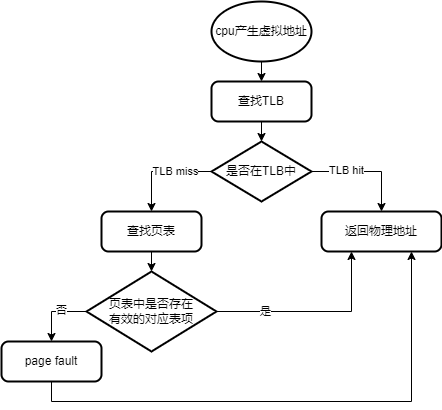
\includegraphics[width=0.5\linewidth]{assets/10/hard-tlb-ctrl.png}
  \caption{基于硬件的TLB管理}
  \label{fig:hard-tlb-ctrl}
\end{figure}

其中，TLB miss后查找页表的这个过程是由硬件自动完成的，软件只需处理后面产生的page fault。整个过程中最多产生一次page fault。

图\ref{fig:soft-tlb-ctrl}则为软件管理TLB方案中虚拟地址转换到物理地址的过程：

\begin{figure}[htbp]
  \centering
  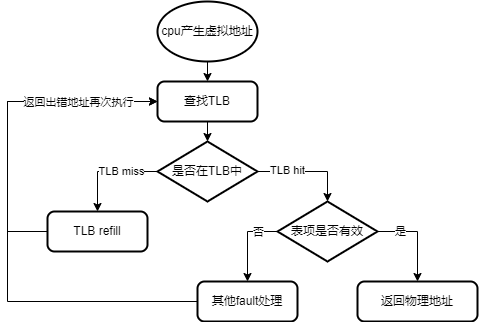
\includegraphics[width=0.5\linewidth]{assets/10/soft-tlb-ctrl.png}
  \caption{基于软件的TLB管理}
  \label{fig:soft-tlb-ctrl}
\end{figure}

具体解释如下：

\begin{enumerate}
\def\labelenumi{\arabic{enumi}.}
\tightlist
\item
  TLB miss后会产生第一次TLB重填（TLB refill）异常，在TLB重填异常中需要软件去遍历页表并填充TLB表项，这里应该是软件管理TLB和硬件管理TLB最大的不同。
\item
  然后TLB重填异常处理中，如果填充的页表项仍然无效，那么在返回后再次查询TLB时，会第二次产生其他的fault处理，以填充页表项、或填充页表项和TLB项。
\item
  如果第二次fault处理中没有重填TLB表项，那么在返回后再次查询TLB时，还会产生第三次TLB重填异常。
\end{enumerate}

可以看到，TLB miss后查找页表的这个过程需要软件进行处理，并且整个过程中最多能产生三次异常。

另外，硬件上会保证在TLB重填异常中不能再次产生TLB重填异常。

\subsection{TLB的软硬件交互机制}\label{sec:10-mmu-004}

TLB的软硬件交互集中体现在TLB相关的异常处理方面，硬件通过异常来处罚相关的软件处理流程，而软件则通过相关指令修复TLB异常。下面结合linux源码对TLB相关异常处理进行分析。

linux中TLB相关异常和相关处理函数的对应关系如下：

\begin{itemize}
\tightlist
\item
  TLB重填异常：handle\_tlb\_refill
\item
  load/取指操作页无效异常：handle\_tlb\_load
\item
  store操作页无效异常：handle\_tlb\_store
\item
  页修改异常：handle\_tlb\_modify
\item
  页不可读/不可写/特权不合规异常：handle\_tlb\_protect
\end{itemize}

这里分析handle\_tlb\_refill、handle\_tlb\_load和handle\_tlb\_protect函数。其中handle\_tlb\_store和handle\_tlb\_modify实际上流程与handle\_tlb\_load基本一致，只是更新页表项时更新的位不同。

\subsubsection{TLB重填异常}\label{sec:10-mmu-005}

TLB重填异常（handle\_tlb\_refill）触发前后硬件中的处理与一般异常存在差异，主要是TLB重填异常相关有独立的一套寄存器。但都会有相应保存和恢复现场、跳转和返回操作。值得注意的是，TLB重填异常中出错的地址保存在CSR.TLBRBADV寄存器，而一般异常出错的地址保存在CSR.BADV寄存器。

TLB重填异常的软件处理过程如下：

\begin{enumerate}
\def\labelenumi{\arabic{enumi}.}
\tightlist
\item
  保存现场
\item
  根据CSR.TLBRBADV中记录的缺失虚拟地址，和CSR.PGD中pgd基址，遍历发生TLB重填异常的进程的多级页表，从内存中取回页表项信息并填入CSR.TLBELO0和CSR.TLBELO1寄存器的相应域中
\item
  根据填入的CSR.TLBELO0和CSR.TLBELO1寄存器信息，最终用tlbfill指令将页表项填入TLB
\item
  恢复并返回
\end{enumerate}

代码分析如下：

% 代码语言：asm
\begin{CodeBlock}
SYM_FUNC_START(handle_tlb_refill)
    csrwr   t0, LOONGARCH_CSR_TLBRSAVE // 将t0保存到CSR.TLBRSAVE寄存器
    csrrd   t0, LOONGARCH_CSR_PGD // 读取pgd基址到t0
    lddir   t0, t0, 3 // 根据CSR.TLBRBADV中记录的缺失虚拟地址，
                      // 访问3级页表，读取2级页表基址到t0（pgd为3级页表基址）
#if CONFIG_PGTABLE_LEVELS > 3
    lddir   t0, t0, 2 // 根据CSR.TLBRBADV中记录的缺失虚拟地址，
                      // 访问2级页表，读取1级页表基址到t0
#endif
#if CONFIG_PGTABLE_LEVELS > 2
    lddir   t0, t0, 1 // 根据CSR.TLBRBADV中记录的缺失虚拟地址，
                      // 访问1级页表，读取末级页表地址或大页到t0
#endif
    ldpte   t0, 0 // 根据CSR.TLBRBADV中记录的缺失虚拟地址，
                  // 访问末级页表或大页，读取偶数号页表项或大页到CSR.TLBELO0
    ldpte   t0, 1 // 根据CSR.TLBRBADV中记录的缺失虚拟地址，
                  // 访问末级页表或大页，读取奇数号页表项或大页到CSR.TLBELO1
    tlbfill // 根据CSR.TLBELO0、CSR.TLBELO1等寄存器中信息，
            // 将页表项填入TLB
    csrrd   t0, LOONGARCH_CSR_TLBRSAVE // 恢复t0
    ertn // 从异常返回
SYM_FUNC_END(handle_tlb_refill)
\end{CodeBlock}

\subsubsection{load/fetch操作页无效异常}\label{sec:10-mmu-006}

load/fetch操作页无效异常触发前后硬件中的处理与一般异常相同。

handle\_tlb\_load处理的过程如下：

\begin{enumerate}
\def\labelenumi{\arabic{enumi}.}
\tightlist
\item
  保存现场
\item
  根据CSR.BADV中记录的缺失虚拟地址，和CSR.PGD中pgd基址，遍历发生异常的进程的多级页表，从内存中取回页表项（或大页）信息
\item
  判断该页表项是否存在，如果不存在则会跳转执行缺页处理函数
\item
  如果存在则将页表项置为有效并填入TLB。最后恢复并返回
\end{enumerate}

代码分析如下：

% 代码语言：asm
\begin{CodeBlock}
SYM_FUNC_START(handle_tlb_load)
    // 将t0、t1、ra写入CSR.SAVE0-CSR.SAVE3，暂存寄存器
    csrwr        t0, EXCEPTION_KS0
    csrwr        t1, EXCEPTION_KS1
    csrwr        ra, EXCEPTION_KS2
    /*
     * The vmalloc handling is not in the hotpath.
     */
    // 如果CSR.BADV不小于0，则继续执行到vmalloc_done_load
    // 将CSR.BADV和CSR.PGDL读入t0和t1
    // 否则跳转到vmalloc_load将CSR.BADV和swapper_pg_dir读入t0和t1
    // 即CSR.BADV不小于0时使用低半部分内核地址的pgd，
    // 否则使用高半部分用户地址的pgd
    csrrd        t0, LOONGARCH_CSR_BADV
    bltz        t0, vmalloc_load
    csrrd        t1, LOONGARCH_CSR_PGDL
vmalloc_done_load:
    /* Get PGD offset in bytes */
    // 根据t0中CSR.BADV地址和t1中pgd基址，遍历页表查找
    bstrpick.d    ra, t0, PTRS_PER_PGD_BITS + PGDIR_SHIFT - 1, PGDIR_SHIFT
    alsl.d        t1, ra, t1, 3
#if CONFIG_PGTABLE_LEVELS > 3
    ld.d        t1, t1, 0
    bstrpick.d    ra, t0, PTRS_PER_PUD_BITS + PUD_SHIFT - 1, PUD_SHIFT
    alsl.d        t1, ra, t1, 3
#endif
#if CONFIG_PGTABLE_LEVELS > 2
    ld.d        t1, t1, 0
    bstrpick.d    ra, t0, PTRS_PER_PMD_BITS + PMD_SHIFT - 1, PMD_SHIFT
    alsl.d        t1, ra, t1, 3
    // 到这里t1中为1级页表（pmd）地址
#endif
    // 将1级页表中第一个表项读取到ra
    ld.d        ra, t1, 0
    /*
     * For huge tlb entries, pmde doesn't contain an address but
     * instead contains the tlb pte. Check the PAGE_HUGE bit and
     * see if we need to jump to huge tlb processing.
     */
    // 如果ra中表项为大页，则跳转到tlb_huge_update_load
    rotri.d        ra, ra, _PAGE_HUGE_SHIFT + 1
    bltz        ra, tlb_huge_update_load

    rotri.d        ra, ra, 64 - (_PAGE_HUGE_SHIFT + 1)
    bstrpick.d    t0, t0, PTRS_PER_PTE_BITS + PAGE_SHIFT - 1, PAGE_SHIFT
    alsl.d        t1, t0, ra, _PTE_T_LOG2
    // 到这里t1中为CSR.BADV对应末级页表项地址

    // 读取页表项到t0
#ifdef CONFIG_SMP
smp_pgtable_change_load:
    ll.d        t0, t1, 0 // smp中使用ll/sc原子指令对循环写入
#else
    ld.d        t0, t1, 0
#endif
    // 如果页表项不存在，则跳转到nopage_tlb_load调用缺页处理函数
    // 否则继续向下执行，写入对应有效的页表项到TLB
    andi        ra, t0, _PAGE_PRESENT
    beqz        ra, nopage_tlb_load

    // 设置有效位并更新页表项
    ori        t0, t0, _PAGE_VALID
#ifdef CONFIG_SMP
    sc.d        t0, t1, 0
    beqz        t0, smp_pgtable_change_load // 写入失败时跳转
#else
    st.d        t0, t1, 0
#endif    
    // 根据CSR.ASID和CSR.TLBEHI的信息查询TLB，以便tlbwr指令写入
    // 如果命中则将其索引写入CSR.TLBIDX，否则将CSR.TLBIDX.NE置为1
    // 这里必然会命中
    tlbsrch

    // t0 = 偶数项页表项，t1 = 奇数项页表项
    bstrins.d    t1, zero, 3, 3
    ld.d        t0, t1, 0
    ld.d        t1, t1, 8
    // 写入TLB相关寄存器
    csrwr        t0, LOONGARCH_CSR_TLBELO0
    csrwr        t1, LOONGARCH_CSR_TLBELO1
    // 根据CSR.TLBELO0、CSR.TLBELO1、CSR.TBLIDX等相关寄存器信息，
    // 将页表项信息写入TLB中CSR.TBLIDX.index对应位置
    tlbwr
    // 恢复并返回
    csrrd        t0, EXCEPTION_KS0
    csrrd        t1, EXCEPTION_KS1
    csrrd        ra, EXCEPTION_KS2
    ertn
#ifdef CONFIG_64BIT
vmalloc_load:
    la.abs        t1, swapper_pg_dir
    b        vmalloc_done_load
#endif
    /* This is the entry point of a huge page. */
tlb_huge_update_load:
    // 对于大页，异常处理的流程和上面基本页表项的处理流程基本一致
    // 只是填入TLB时会做一些额外的格式转换处理等，这里不再赘述
    ...
nopage_tlb_load:
    dbar        0
    csrrd        ra, EXCEPTION_KS2
    la.abs        t0, tlb_do_page_fault_0
    jr        t0
SYM_FUNC_END(handle_tlb_load)
\end{CodeBlock}

\subsubsection{页不可读/不可写/特权不合规异常}\label{sec:10-mmu-007}

页不可读/不可写/特权不合规异常触发前后硬件中的处理与一般异常相同。

handle\_tlb\_protect处理的过程实际上就是调用缺页处理函数，来填入页表。

代码分析如下：

% 代码语言：asm
\begin{CodeBlock}
SYM_FUNC_START(handle_tlb_protect)
    // 保存寄存器
    BACKUP_T0T1
    SAVE_ALL
    // 设置传参
    move    a0, sp
    move    a1, zero
    csrrd    a2, LOONGARCH_CSR_BADV
    REG_S    a2, sp, PT_BVADDR
    // 调用do_page_fault
    la.abs    t0, do_page_fault
    jirl    ra, t0, 0
    // 恢复并返回
    RESTORE_ALL_AND_RET
SYM_FUNC_END(handle_tlb_protect)
\end{CodeBlock}

\section{TLB模块设计}\label{sec:10-mmu-008}

在考虑TLB模块的内部设计时，重点是查找、读和写三套操作的实现。读和写操作可以参考CPU中寄存器文件（regfile）的逻辑设计和Verilog代码实现。本文将主要介绍查找操作的设计实现。

\textbf{读和写操作}

TLB模块的读写接口上的PS域是6比特的，但由于LoongArch精简版中只支持4KB和4MB两种页大小，因此TLB模块内部仅用1比特来存储这两种页大小信息，需要进行一个简单的转换。读和写操作实现可以借鉴CPU寄存器文件的逻辑设计和Verilog代码实现，不再赘述。

\textbf{查找操作}

指令手册中的TLB查找流程伪算法描述是串行化的，但在实际电路实现时，我们并不是先比较第0项、再比较第1项\ldots\ldots 而是同时比较所有项。假设TLB有16项，需要通过组合逻辑产生一个16位宽的查找结果\texttt{match{[}15:0{]}}。这个结果的第0位对应第0项的比较结果，第1位对应第1项的比较结果，以此类推。

下面是查找操作的伪代码示意：

% 代码语言：pseudocode
\begin{CodeBlock}
# 初始TLB未找到标志
tlb_found = 0

# 遍历TLB条目
for i in range(TLB_ENTRIES):
    # 检查当前TLB条目是否有效，且全局标志位为1或ASID匹配，且虚拟页号匹配
    if (TLB[i].E == 1) and ((TLB[i].G == 1) or (TLB[i].ASID == CSR.ASID.ASID)) and \
       (TLB[i].VPPN[VALEN-1: TLB[i].PS+1] == va[VALEN-1: TLB[i].PS+1]):
        
        # 如果之前没有找到匹配的TLB条目
        if tlb_found == 0:
            tlb_found = 1
            found_ps = TLB[i].PS

            # 根据虚拟地址的页偏移选择对应的TLB条目字段
            if va[found_ps] == 0:
                found_v = TLB[i].V0
                found_d = TLB[i].D0
                found_mat = TLB[i].MAT0
                found_plv = TLB[i].PLV0
                found_ppn = TLB[i].PPN0
            else:
                found_v = TLB[i].V1
                found_d = TLB[i].D1
                found_mat = TLB[i].MAT1
                found_plv = TLB[i].PLV1
                found_ppn = TLB[i].PPN1
        else:
            # 出现多项命中，处理器运行结果不确定
            # 这里可能需要添加相关处理逻辑

# 如果没有找到匹配的TLB条目，触发TLB重填例外
if tlb_found == 0:
    SignalException(TLBR)

# 如果找到的条目无效，根据访问类型触发相应的例外
if found_v == 0:
    if mem_type == 'FETCH':
        SignalException(PIF)  # 取指操作页无效例外
    elif mem_type == 'LOAD':
        SignalException(PIL)  # 读取操作页无效例外
    elif mem_type == 'STORE':
        SignalException(PIS)  # 存储操作页无效例外

# 如果访问的特权等级超过页表项的特权等级，触发页特权等级不合规例外
elif plv > found_plv:
    SignalException(PPI)

# 如果是存储操作且页面未修改，触发页修改例外
elif mem_type == 'STORE' and found_d == 0:
    SignalException(PME)

# 否则计算物理地址并设置内存属性
else:
    pa = {found_ppn[PALEN-13:found_ps-12], va[found_ps-1:0]}
    mat = found_mat

\end{CodeBlock}

要生成查询比较结果，首先需确定是否命中。这可以通过检查匹配结果是否全为零来判断。如果匹配结果不全为零，则表示有命中项。命中项的物理页号（PFN）等信息的读取逻辑也相对简单。

接下来，我们分析INVTLB指令所需的查找操作支持。由于当前TLB实现采用并行查找机制进行虚拟地址到物理地址的转换，因此INVTLB指令的查找也将采用并行查找机制，即同时对TLB中的各项进行匹配判断。设计的关键在于如何处理每一项的匹配。通过分析INVTLB指令的操作定义，我们可以将各操作的匹配分解为若干``子匹配''逻辑组合。具体来说，有四个``子匹配''的判断条件：

\begin{enumerate}
\def\labelenumi{\arabic{enumi}.}
\item
  cond1------G域是否等于0；
\item
  cond2------G域是否等于1；
\item
  cond3------s1\_asid是否等于ASID域；
\item
  cond4------s1\_vppn是否匹配VPPN和PS域。
\end{enumerate}

在此基础上，不同操作的匹配条件可以表达如下：

\begin{itemize}
\tightlist
\item
  对于op=0和op=1，匹配条件为cond1或cond2；
\item
  对于op=4，匹配条件为cond1且cond3；
\item
  对于op=5，匹配条件为cond1且cond3且cond4；
\item
  对于op=6，匹配条件为（cond2或cond3）且cond4。
\end{itemize}

值得注意的是，op=6的匹配条件正是取指和访存进行虚实地址转换时的查找匹配条件，因此这两类操作的查找匹配功能可以统一到同一逻辑中。两者的区别仅在于基于查找结果所采取的进一步操作。对于INVTLB指令，将相应TLB表项无效化的操作是将inv\_match{[}i{]}等于1对应的tlb\_e{[}i{]}置为0。

\section{TLB相关的寄存器与指令}\label{sec:10-mmu-009}

\subsection{TLB相关的CSR寄存器}\label{sec:10-mmu-010}

在LoongArch架构下，关于TLB（转换后备缓冲区）相关的控制状态寄存器（CSR）有以下几个重要的寄存器：

\begin{enumerate}
\def\labelenumi{\arabic{enumi}.}
\tightlist
\item
  \textbf{CSR.ASID}：这是地址空间标识符寄存器，用于标识不同的地址空间。每个TLB条目与一个特定的ASID相关联，这样可以在不清空TLB的情况下进行上下文切换。
\item
  \textbf{CSR.TLBEHI}：TLB入口高位寄存器，存储虚拟地址的高位部分以及其他一些控制信息。用于查询和操作TLB条目时提供所需的地址信息。
\item
  \textbf{CSR.TLBELO0 和 CSR.TLBELO1}：这两个寄存器分别存储TLB条目的低位部分，包括物理地址和页表项的其他标志。TLBELO0和TLBELO1分别对应一个TLB条目的两个物理页框地址。
\item
  \textbf{CSR.TLBIDX}：这是TLB索引寄存器，包含用于指定TLB条目索引的字段。还包括一个指示TLB条目是否有效的标志位（INV）。
\end{enumerate}

更详细的介绍请参看LoongArch精简指令集手册。

\subsection{TLB相关的指令}\label{sec:10-mmu-011}

以下表格总结了LoongArch指令集架构中用于TLB管理和维护的指令：

\begin{longtable}[]{@{}
  >{\raggedright\arraybackslash}p{(\linewidth - 4\tabcolsep) * \real{0.0870}}
  >{\raggedright\arraybackslash}p{(\linewidth - 4\tabcolsep) * \real{0.5217}}
  >{\raggedright\arraybackslash}p{(\linewidth - 4\tabcolsep) * \real{0.3913}}@{}}
\toprule\noalign{}
\begin{minipage}[b]{\linewidth}\raggedright
指令
\end{minipage} & \begin{minipage}[b]{\linewidth}\raggedright
描述
\end{minipage} & \begin{minipage}[b]{\linewidth}\raggedright
使用示例
\end{minipage} \\
\midrule\noalign{}
\endhead
\bottomrule\noalign{}
\endlastfoot
\texttt{tlbsrch} & 查询TLB对应的索引。使用CSR.ASID和CSR.TLBEHI中的信息查询TLB，如果命中则将其对应索引写入CSR.TLBIDX.Index，否则将CSR.TLBIDX.NE置为1。 & \texttt{tlbsrch}指令查询TLB中是否包含特定的页表项。 \\
\texttt{tlbrd} & 读取索引对应的TLB表项。将CSR.TLBIDX.Index作为索引，读取TLB中的指定项。如果该TLB项有效，则将其页表项信息写入CSR.TLBEHI、CSR.TLBELO0、CSR.TLBELO1和CSR.TLBINX.PS寄存器，并将CSR.TLBIND.NE置0；如果无效，则将CSR.TLBIND.NE置1。 & \texttt{tlbrd}指令读取TLB中的特定表项信息。 \\
\texttt{tlbwr} & 写入索引对应的TLB表项。将CSR.TLBIDX.Index作为索引，把CSR.TLBEHI、CSR.TLBELO0、CSR.TLBELO1和CSR.TLBINX.PS中的页表项信息写入TLB中的指定项。如果CSR.TLBIND.NE置为1，则写入的是一个无效的TLB项。 & \texttt{tlbwr}指令将页表项信息写入TLB中的指定位置。 \\
\texttt{tlbfill} & 类似于\texttt{tlbwr}指令，不同的是\texttt{tlbfill}写入TLB位置由硬件随机决定。 & \texttt{tlbfill}指令随机插入页表项到TLB中。 \\
\texttt{tlbclr} & 根据TLB相关CSR中的信息无效化TLB中的内容。 & \texttt{tlbclr}指令无效化TLB中的特定表项。 \\
\texttt{tlbflush} & 根据TLB相关CSR中的信息无效化TLB中的内容，但作用范围较\texttt{tlbclr}更广。 & \texttt{tlbflush}指令无效化TLB中的所有表项。 \\
\texttt{invtlb} & 用于无效化TLB中的内容，比\texttt{tlbclr}和\texttt{tlbflush}指令更加灵活。 & \texttt{invtlb}指令用于灵活地无效化TLB中的特定表项。 \\
\end{longtable}

\section{利用TLB进行虚实地址转换}\label{sec:10-mmu-012}

\subsection{地址翻译}\label{sec:10-mmu-013}

下面我们主要介绍LoongArch架构下是如何进行虚拟地址翻译的。

\subsubsection{地址空间}\label{sec:10-mmu-014}

在LoongArch架构中，虚拟地址空间和物理地址空间的大小如下：

\textbf{虚拟地址空间}

\begin{itemize}
\tightlist
\item
  \textbf{LA32}：虚拟地址空间大小为 2\textsuperscript{32} 字节。
\item
  \textbf{LA64}：虚拟地址空间大小为 2\textsuperscript{64} 字节。
\end{itemize}

\textbf{物理地址空间}

\begin{itemize}
\tightlist
\item
  \textbf{LoongArch中的物理地址空间大小为} 2\textsuperscript{PALEN} 字节，其中：

  \begin{itemize}
  \tightlist
  \item
    \textbf{LA32}：PALEN为一个不超过36的正整数，通常为32。
  \item
    \textbf{LA64}：PALEN为一个不超过60的正整数。
  \end{itemize}
\end{itemize}

PALEN由具体实现决定，软件可以通过CPUCFG指令读取PALEN的值。

\subsubsection{地址翻译模式}\label{sec:10-mmu-015}

loongarch中通过控制寄存器CSR.CRMD配置地址翻译模式：

\begin{itemize}
\tightlist
\item
  CSR.CRMD中DA=1且PG=0：直接地址翻译模式
\item
  CSR.CRMD中DA=0且PG=1：映射地址翻译模式
\item
  其他DA和PG值的组合的行为未定义
\end{itemize}

下表是这两个寄存器的详细定义

\begin{longtable}[]{@{}
  >{\raggedright\arraybackslash}p{(\linewidth - 6\tabcolsep) * \real{0.0556}}
  >{\raggedright\arraybackslash}p{(\linewidth - 6\tabcolsep) * \real{0.0556}}
  >{\raggedright\arraybackslash}p{(\linewidth - 6\tabcolsep) * \real{0.0556}}
  >{\raggedright\arraybackslash}p{(\linewidth - 6\tabcolsep) * \real{0.8333}}@{}}
\toprule\noalign{}
\begin{minipage}[b]{\linewidth}\raggedright
位
\end{minipage} & \begin{minipage}[b]{\linewidth}\raggedright
名称
\end{minipage} & \begin{minipage}[b]{\linewidth}\raggedright
RW
\end{minipage} & \begin{minipage}[b]{\linewidth}\raggedright
描述
\end{minipage} \\
\midrule\noalign{}
\endhead
\bottomrule\noalign{}
\endlastfoot
3 & DA & RW & 直接地址翻译模式的使能，高有效。\newline{}当触发 TLB 重填例外时，硬件将该域置为 1。\newline{}当执行 ERTN 指令从例外处理程序返回时，如果 CSR.ESTAT.Ecode=0x3F，则硬件将该域置为 0。\newline{}DA 位和 PG 位的合法组合情况为 0, 1 或 1, 0，当软件配置成其它组合情况时结果不确定。 \\
4 & PG & RW & 映射地址翻译模式的使能，高有效。\newline{}当触发 TLB 重填例外时，硬件将该域置为 0。\newline{}当执行 ERTN 指令从例外处理程序返回时，如果 CSR.ESTAT.Ecode=0x3F，则硬件将该域置为 1。\newline{}PG 位和 DA 位的合法组合情况为 0, 1 或 1, 0，当软件配置成其它组合情况时结果不确定。 \\
\end{longtable}

LoongArch架构中的虚实地址转换机制由其地址翻译模式确定。LoongArch中有以下两种地址翻译模式：

\begin{enumerate}
\def\labelenumi{\arabic{enumi}.}
\item
  \textbf{直接地址翻译模式}：

  \begin{itemize}
  \tightlist
  \item
    在该模式下，物理地址直接等于虚拟地址的低PALEN位，不足部分补0。此模式相当于没有进行映射。
  \end{itemize}
\item
  \textbf{映射地址翻译模式}：

  \begin{itemize}
  \tightlist
  \item
    该模式下又分为两种子模式：

    \begin{itemize}
    \item
      \textbf{直接映射地址翻译模式（直接映射模式）}：

      LoongArch中的直接映射模式是一种线性的映射方式，有点类似于分段。通过配置直接映射配置窗口寄存器，可以实现直接映射。

      共有4个直接映射配置窗口寄存器，分别为CSR.DMW0到CSR.DMW3。配置一个窗口相当于映射一段内存区域。其中：

      \begin{itemize}
      \tightlist
      \item
        \textbf{CSR.DMW0}和\textbf{CSR.DMW1}：

        \begin{itemize}
        \tightlist
        \item
          映射的内存区域可以同时用于取指和load/store操作。
        \end{itemize}
      \item
        \textbf{CSR.DMW2}和\textbf{CSR.DMW3}：

        \begin{itemize}
        \tightlist
        \item
          映射的内存区域仅用于load/store操作。
        \end{itemize}
      \end{itemize}

      通过这些配置窗口寄存器，用户可以灵活地定义虚拟地址到物理地址的直接映射区域，以满足不同的内存访问需求。
    \item
      \textbf{页表映射地址翻译模式（页表映射模式）}：

      在LoongArch架构中，可以同时有两个页全局目录（PGD）基址，这两个基址分别存储于寄存器CSR.PGDL（低半地址空间全局目录基址）和CSR.PGDH（高半地址空间全局目录基址），分别对应低半地址空间和高半地址空间。低半地址空间和高半地址空间实际上是将虚拟地址空间对半分成两个部分：

      \begin{itemize}
      \tightlist
      \item
        \textbf{低半地址空间}：

        \begin{itemize}
        \tightlist
        \item
          虚拟地址的最高位为0。
        \item
          使用CSR.PGDL中的基址进行地址转换。
        \end{itemize}
      \item
        \textbf{高半地址空间}：

        \begin{itemize}
        \tightlist
        \item
          虚拟地址的最高位为1。
        \item
          使用CSR.PGDH中的基址进行地址转换。
        \end{itemize}
      \end{itemize}

      两个部分的地址转换互不干扰，各自使用对应的PGD。在Linux中：

      \begin{itemize}
      \tightlist
      \item
        \textbf{CSR.PGDH}：存放内核进程的PGD。
      \item
        \textbf{CSR.PGDL}：存放用户进程的PGD。
      \end{itemize}

      这种设计在硬件上实现了对内核空间和用户空间的页表隔离，提高了系统的安全性和稳定性。
    \end{itemize}
  \end{itemize}
\end{enumerate}

\textbf{总之：}

直接地址翻译模式和映射地址翻译模式不能同时启用。在映射地址翻译模式下，可以同时启用直接映射模式和页表映射模式。在进行地址翻译时，系统会优先使用直接映射模式，如果无法使用直接映射模式，则使用页表映射模式进行翻译。

LoongArch架构的地址翻译机制通过配置不同的地址翻译模式实现虚拟地址到物理地址的转换，具有灵活性和高效性。通过合理配置CSR.CRMD寄存器中的DA和PG位，用户可以根据需求选择直接地址翻译模式或映射地址翻译模式，从而实现不同的内存访问需求和系统性能优化。

\subsection{TLB接口设计}\label{sec:10-mmu-016}

页表映射模式的核心组件便是TLB，通过梳理TLB模块相关知识，并结合CPU流水线的结构特点，我们对TLB模块的设计分析如下：

\begin{enumerate}
\def\labelenumi{\arabic{enumi}.}
\tightlist
\item
  \textbf{查找表结构}：

  \begin{itemize}
  \tightlist
  \item
    TLB模块的主体应为一个二维组织结构的查找表。每一项分为两部分：

    \begin{itemize}
    \tightlist
    \item
      第一部分存储的信息既参与读写又参与查找比较，包括E、VPPN、PS、ASID和G。
    \item
      第二部分仅参与读写，包括PPN0、PLV0、MAT0、D0、V0、PPN1、PLV1、MAT1、D1、V1。
    \end{itemize}
  \item
    查找表的项数由实现者自行定义。
  \end{itemize}
\item
  \textbf{虚实地址转换支持}：

  \begin{itemize}
  \tightlist
  \item
    TLB模块要支持取指和访存的虚实地址转换需求，两个部分都需要对TLB模块进行查找，且查找功能一致。
  \item
    查找时，向TLB模块输入s\_vppn、s\_va\_bit12和s\_asid信息，输出信息包括s\_found、s\_ppn、s\_ps、s\_plv、s\_mat、s\_d和s\_v。
  \item
    输入信息：

    \begin{itemize}
    \tightlist
    \item
      s\_vppn来自访存虚地址的31..13位，
    \item
      s\_va\_bit12来自访存虚地址的12位，
    \item
      s\_asid来自CSR.ASID的ASID域。
    \end{itemize}
  \item
    输出信息：

    \begin{itemize}
    \tightlist
    \item
      s\_ppn和s\_ps用于产生最终的物理地址，
    \item
      s\_found用于判定是否产生TLB重填异常，
    \item
      s\_found和s\_v用于判定是否产生页无效异常，
    \item
      s\_found和s\_plv用于判定是否产生页特权等级不合规异常，
    \item
      s\_found、s\_v和s\_d用于判定是否产生页修改异常。
    \end{itemize}
  \end{itemize}
\item
  \textbf{并行查找支持}：

  \begin{itemize}
  \tightlist
  \item
    为了使流水线能够满负荷运转不断流，TLB模块要能够支持取指和访存同时进行查找。这意味着查找端口应该有两套。
  \end{itemize}
\item
  \textbf{TLBSRCH指令支持}：

  \begin{itemize}
  \tightlist
  \item
    TLB模块需要支持TLBSRCH指令的查找操作，建议复用访存指令查找TLB的端口，输入复用s\_vppn和s\_asid，输出复用已有的s\_found。
  \item
    需要一个额外的s\_index输出，用于记录命中在第几项，其信息用于填入到CSR.TLBIDX中。
  \end{itemize}
\item
  \textbf{TLBWR和TLBFILL指令支持}：

  \begin{itemize}
  \tightlist
  \item
    TLB模块需要支持TLBWR和TLBFILL指令的写操作，建议为此设计独立的端口。
  \item
    输入信息包括写地址w\_index，写入的TLB表项信息w\_e、w\_vppn、w\_ps、w\_asid、w\_g、w\_ppn0、w\_plv0、w\_mat0、w\_d0、w\_v0、w\_ppn1、w\_plv1、w\_mat1、w\_d1、w\_v1。
  \item
    写操作需有写使能输入信号we。
  \end{itemize}
\item
  \textbf{TLBRD指令支持}：

  \begin{itemize}
  \tightlist
  \item
    TLB模块需要支持TLBRD指令的读操作，建议为此设计独立的端口。
  \item
    输入信息包括读地址r\_index。
  \item
    输出结果有r\_e、r\_vppn、r\_ps、r\_asid、r\_g、r\_ppn0、r\_plv0、r\_mat0、r\_d0、r\_v0、r\_ppn1、r\_plv1、r\_mat1、r\_d1、r\_v1。
  \end{itemize}
\item
  \textbf{INVTLB指令支持}：

  \begin{itemize}
  \tightlist
  \item
    TLB模块需要支持INVTLB指令的查找和无效操作。
  \item
    不同操作类型的查找信息可复用访存指令查找TLB的端口，仅需一个额外的invtlb\_op输入，用于标识具体操作类型。
  \item
    invtlb的无效操作在TLB模块内部根据查找结果直接将符合条件的TLB表项的E位置为0。
  \end{itemize}
\end{enumerate}

通过上述分析，我们得到TLB模块的接口与内部主要信号的定义如下：

% 代码语言：verilog
\begin{CodeBlock}
module tlb
#(
    parameter TLBNUM = 16
)
(
    input  wire                      clk,

    // search port 0 (for fetch)
    input  wire [              18:0] s0_vppn,
    input  wire                      s0_va_bit12,
    input  wire [               9:0] s0_asid,
    output wire                      s0_found,
    output wire [$clog2(TLBNUM)-1:0] s0_index,
    output wire [              19:0] s0_ppn,
    output wire [               5:0] s0_ps,
    output wire [               1:0] s0_plv,
    output wire [               1:0] s0_mat,
    output wire                      s0_d,
    output wire                      s0_v,

    // search port 1 (for load/store)
    input  wire [              18:0] s1_vppn,
    input  wire                      s1_va_bit12,
    input  wire [               9:0] s1_asid,
    output wire                      s1_found,
    output wire [$clog2(TLBNUM)-1:0] s1_index,
    output wire [              19:0] s1_ppn,
    output wire [               5:0] s1_ps,
    output wire [               1:0] s1_plv,
    output wire [               1:0] s1_mat,
    output wire                      s1_d,
    output wire                      s1_v,

    // invtlb opcode
    input  wire                      invtlb_valid,
    input  wire [               4:0] invtlb_op,

    // write port
    input  wire                      we,     //w(rite) e(nable)
    input  wire [$clog2(TLBNUM)-1:0] w_index,
    input  wire                      w_e,
    input  wire [              18:0] w_vppn,
    input  wire [               5:0] w_ps,
    input  wire [               9:0] w_asid,
    input  wire                      w_g,
    input  wire [              19:0] w_ppn0,
    input  wire [               1:0] w_plv0,
    input  wire [               1:0] w_mat0,
    input  wire                      w_d0,
    input  wire                      w_v0,
    input  wire [              19:0] w_ppn1,
    input  wire [               1:0] w_plv1,
    input  wire [               1:0] w_mat1,
    input  wire                      w_d1,
    input  wire                      w_v1,

    // read port
    input  wire [$clog2(TLBNUM)-1:0] r_index,
    output wire                      r_e,
    output wire [              18:0] r_vppn,
    output wire [               5:0] r_ps,
    output wire [               9:0] r_asid,
    output wire                      r_g,
    output wire [              19:0] r_ppn0,
    output wire [               1:0] r_plv0,
    output wire [               1:0] r_mat0,
    output wire                      r_d0,
    output wire                      r_v0,
    output wire [              19:0] r_ppn1,
    output wire [               1:0] r_plv1,
    output wire [               1:0] r_mat1,
    output wire                      r_d1,
    output wire                      r_v1
);

reg  [TLBNUM-1:0] tlb_e;
reg  [TLBNUM-1:0] tlb_ps4MB; //pagesize 1:4MB, 0:4KB
reg  [      18:0] tlb_vppn     [TLBNUM-1:0];
reg  [       9:0] tlb_asid     [TLBNUM-1:0];
reg               tlb_g        [TLBNUM-1:0];
reg  [      19:0] tlb_ppn0     [TLBNUM-1:0];
reg  [       1:0] tlb_plv0     [TLBNUM-1:0];
reg  [       1:0] tlb_mat0     [TLBNUM-1:0];
reg               tlb_d0       [TLBNUM-1:0];
reg               tlb_v0       [TLBNUM-1:0];
reg  [      19:0] tlb_ppn1     [TLBNUM-1:0];
reg  [       1:0] tlb_plv1     [TLBNUM-1:0];
reg  [       1:0] tlb_mat1     [TLBNUM-1:0];
reg               tlb_d1       [TLBNUM-1:0];
reg               tlb_v1       [TLBNUM-1:0];

......

endmodule
\end{CodeBlock}

% !TeX root = ../main.tex
% 原始章节：11-advenced-cpu.Rmd

\chapter{处理器性能优化}\label{chap:11-advanced-cpu}

对于处理器运行特定测试程序时的性能，通常以执行时间对其进行评价。
对于相同的体系结构，运行特定程序可以视为执行了相同的指令序列。因此对特定测试程序和特定体系结构，程序的执行时间与只与处理器每单位时间内可以执行的指令数量相关。

因此要改提升通用处理器性能，实际就是提高处理器执行指令的吞吐量。
处理器每单位时间内可以执行的指令数量，实际就等于处理器的运行频率乘以平均每周期执行的指令数。
提高处理器性能即提高处理器的运行频率、提高处理器每周期执行的指令数（IPC）。

\section{处理器运行频率优化}\label{sec:11-advanced-cpu-001}

\subsection{存储部件优化}\label{sec:11-advanced-cpu-002}

处理器内部，存在大量的存储部件。如指令缓存、数据缓存、跳转目标地址缓冲器等等。
这些存储部件，随着处理器规模扩大，往往也有较大的容量和低延迟需求。
这些存储部件常使用 SRAM 实现。 SRAM 存储单元由六个晶体管组成，其中内部四个晶体管组成两个反相器。
这两个反相器耦合，形成一个环路。在无其它输入的情况下保持稳态，整体对外表现为弱驱动。
SRAM 中的另外两个晶体管，用于控制从 SRAM 中读出数据，或通过外部强驱动破坏内部弱驱动稳态，写入新的数据。

SRAM 器件的输出，来自内部六管晶体管组成的两个耦合反相器。且为了保证外部强驱动可以写入新数据，两个耦合反相器输出高电平的驱动能力往往较弱。
SRAM 部件的特殊特性，导致其速度一定慢于锁存器结构的数据存储单元。

处理器内部，大量的大容量 SRAM ，往往会成为处理器频率的一个瓶颈。为了解决这种瓶颈，处理器设计者需要从两个角度对设计进行优化。
首先，可以优化存储部件本身。如一些商业处理器设计者，会对 SRAM 进行全定制设计，以牺牲面积或者静态功耗为代价，加强 SRAM 驱动性能等，根据处理器实际需求寻找一个均衡的设计点。
不具备相似定制设计条件下，可以在设计中规避时序较差的存储部件，如延长读取写入占用的周期数等等，以避免存储部件中占用过大的时序，造成设计时序紧张。

现代处理器，往往也具有大量的大容量多口寄存器堆设计。这些寄存器堆往往占用面积大、功耗大、时序糟糕。
对寄存器堆进行定制设计，也是处理器运行频率优化的重要环节之一。
和 SRAM 一样，商业处理器设计者对于寄存器堆，往往会进行定制设计。根据需要的容量和端口数量以及尺寸约束时序约束，绘制专门的存储单元，控制单元，生成版图。
若不具备定制条件的条件，仅能进行逻辑综合，也应在 RTL 级别尝试对寄存器堆进行一些优化。
寄存器堆的面积，往往与写端口数量的平方成正比。而过大的面积，会带来较困难的布线进一步影响寄存器堆运行频率。
因此，对于设计者来说，尽量使用容量较小、端口较少的寄存器堆也是频率优化的重要环节之一。

有时，处理器出于性能考虑，不得不需要使用多口寄存器堆，这时可以尝试复制的策略构建多口寄存器堆以优化时序和面积情况。

对于多读端口，由于读的操作是幂等的，只需要简单的复制多组相同写端口数量的寄存器堆即可，读取端口自然得到了倍增。
但对于非幂等的写端口，多端口设计则较麻烦。一种常用的方案是 LVT（Live Value Table），使用小容量多写口寄存器堆与多个单写口寄存器堆构建多写口寄存器堆。
这种方案中，有多少个写端口，就复制几组寄存器堆。同时准备一个真多写口的小容量寄存器堆（LVT）记录最新的值位于哪个寄存器堆中。

在读写端口之外，对存储单元的优化也较为重要。每个存储单元记录一位数据，对于寄存器堆而言，存储单元的复杂度和面积占用，决定了整体的面积和时序情况。
即使无法进行专门的定制设计，也可以进行半定制操作，直接使用标准单元结构描述寄存器堆，及实际存储单元。
如，可以直接使用锁存器，避免使用寄存器组成寄存器堆。锁存器与寄存器均可存储数据，但可节约一半的晶体管。
半定制设计，可以直接采用厂家提供的标准单元库完成整个寄存器堆的搭建，以实现频率和面积的优化。当然完成相应设计后，需要进行更为复杂的时序和功能正确性验证。

\subsection{平衡各级流水线的延迟}\label{sec:11-advanced-cpu-003}

体系结构设计中，存在明显的``木桶效应''。处理器性能的瓶颈，往往受制于最短板的一部分。
对于处理器频率的优化也是一样的。处理器频率，只受制于流水线中，时序最紧张的一级。
因此，对于一个确定的微架构，整体逻辑复杂度是确定的。根据简单的不等式关系可以知道，只有当每级流水线延迟均近似相等时，处理器才有最优的运行频率。

这一部分，需要频繁的结合逻辑综合工具，及后端布局布线的时序反馈，对设计进行反思改进。当然，一些过往设计的经验也值得参考。
现有的商业处理器，一般有较为均匀的流水线切分策略，也可以对这些成熟的微体系结构进行参考。
但整体而言，依然是一个需要在实践中发现理解的过程。多编码，多综合，多查看报告是唯一可行路径。

需要注意的是，最终目标并不是需要处理器主频尽可能高，而是要各个寄存器之间切分的组合逻辑时序尽可能接近。
如果一个设计中，某一级流水线成为时序瓶颈，且难以进一步拆分或者优化，那一种可能的正确选择是尝试合并其它流水级，创建尽可能平均的时序延迟分布。
较短的流水线，往往意味着更短的指令执行延迟，更快的分支响应速度。也对性能有很大正面的帮助。

\subsection{弹性流水线}\label{sec:11-advanced-cpu-004}

在很多的流水线设计中，较长的 ready 前馈信号组合逻辑链是限制频率的一大因素。
流水线中，每一级拉高前级流水线 ready 信号的条件，是本级流水线空或者下级流水线 ready 拉高且未阻塞。

这就带来一个问题，每一级流水线的 ready 信号均依赖下一级流水线的 ready 信号。
可若直接去除这个依赖，仅当本级流水线空的时候才拉高 ready 信号，那么流水线中又会出现一半的空泡，严重限制流水线的性能。

因此在实践中，我们往往会构建弹性流水线。所谓弹性流水线，即使用一些先入先出队列（FIFO），替换原有的流水线寄存器。
对于 FIFO 而言，反馈给前级的流水线就绪信号，可以仅与当前 FIFO 容量相关。同时，只要 FIFO 容量大于等于 2，则处理器依然可以保持相同的满速率无空泡运行。
使用 FIFO 替代流水线寄存器，打断 ready 前馈级连构建弹性流水线，也是处理器频率优化的一大必备措施。

\subsection{逻辑复制}\label{sec:11-advanced-cpu-005}

处理器设计中，会出现部分电路具有较大的 FANOUT 的现象。较大的 FANOUT 带来较高的线负载，受限于逻辑元件的驱动能力也会降低处理器频率。
一种做法是，为 FANOUT 严重的关键电路进行逻辑复制，降低 FANOUT 提高处理器频率。

除了 FANOUT 的情况，还有一些时候，电路会由于布局问题带来严重的时序瓶颈。
如 TLB 设计，如指令和数据访存共用同一套 TLB 组件。指令和数据访存由于设计自身原因，在布局上距离较远。
如果两套距离较远的逻辑同时调用 TLB 组件，那么 TLB 组件的布局也将成为一大问题。
这里一般也会采用逻辑复制，将 TLB 复制一份，避免较远的布局复杂度。

逻辑复制，往往会带来较大的面积和功率开销。因此在使用相应的思路对电路优化前，一定要再三进行权衡。只有在非做不可的情况下，再进行相应的工作。

\section{超标量技术}\label{sec:11-advanced-cpu-006}

前文提到，处理器的性能由每周期可执行的指令数（IPC） * 运行频率决定。因此，提高处理器每周期可以执行的指令数也是提高处理器性能的一大方法。
处理器设计者们，因此引入了超标量执行技术，允许流水线在一个周期内执行多于一条指令，以提高处理器的性能。

\subsection{超标量设计引入的冲突及解决}\label{sec:11-advanced-cpu-007}

对比顺序标量核心，超标量核心其实只是多具备了每周期执行更多指令的能力。对比标量核心，超标量顺序核心可以认为只是增加了一条指令执行流水而已。

当然，每周期执行两条指令的流水线承载能力，会导致流水线中引入更多的数据冲突、控制冲突、结构冲突。我们首先对这些冲突，及其解除进行简介

\subsubsection{数据冲突}\label{sec:11-advanced-cpu-008}

新引入的数据冲突主要是在每周期同时送入管线执行的两条指令之间发生的。

同时执行的两条指令可能存在 RAW 的数据真依赖，即第二条指令依赖第一条指令执行结果，则第二条指令一定需要等待第一条指令执行结束后才能开始执行。

两条指令也可能存在 WAW 或者 WAR 的数据伪依赖。对于 WAR 的情况，需要注意前序的读不能读到后续指令写的结果。对于 WAW 的冲突，需要注意写入寄存器的值为最新值。

对于 WAW 及 WAR 冲突，在顺序执行的超标量流水线中稍加注意就不会导致问题，但对于 RAW 的真依赖，则需要特别注意和处理。

一种常见的解决方案是阻止两条存在 RAW 真依赖的指令同时发射执行。一些特殊的处理器，对于一些特殊的相关指令，也允许两条指令同时执行，在执行过程中解决真依赖问题。

\subsubsection{控制冲突}\label{sec:11-advanced-cpu-009}

新引入的指令，也为处理器控制流的处理带来了困难。比如两条同时发射的指令均为跳转指令、两条同时发射的指令均发生了异常跳转等等，这里有比较多可能的特殊情况。

一种可能的设计方案是实现比较复杂的检查机制，允许两条指令同时发出控制流转移请求，综合两条指令的控制流转移请求情况，使用一套比较复杂的组合逻辑确定两条指令如果按顺序执行的结果如何，并采用顺序执行的结果进行执行。

另一种可能的设计方案是限制控制冲突发生。即处理器核心虽支持每周期发射执行两条指令，但其中仅有一条指令允许发生分支或异常，另外一条流水线只允许执行一定不发生异常中断或者跳转的指令。

如此一来，在控制流转移方面的设计，超标量处理器就与标量处理器没有任何区别，不用再考虑复杂的特殊情况去做单独的处理了。

\subsubsection{结构冲突}\label{sec:11-advanced-cpu-010}

处理器实际执行的指令分布往往是不均匀的，整数的简单计算（加减与或）会比乘除有更高的出现频率，而乘除法又比较占用硬件的资源。
因此，在硬件设计中，对于较少执行的指令，往往只会提供少于流水线最大宽度的单元数量和吞吐能力。若处理器要在同一个周期执行的两条乘除指令，就存在结构冲突。

对于结构冲突的解决也比较简单，在静态调度的超标量处理器中，处理器核不允许两条存在结构冲突的指令同时发射，以此规避了所有可能的结构冲突存在。

对于超标量处理器，一般我们定义其宽度为流水线中最窄的一级。因此，保证整个流水线中的通路宽度，保证流水线各处均不窄于设计宽度是设计超标量处理器的关键一步。

\subsection{双取指设计}\label{sec:11-advanced-cpu-011}

在标量处理器中，取指单元只需要每周期产生一个 PC ，并根据 PC 完成取指，拿到一条指令即可。对于超标量处理器，每周期需要产生至少两个预计将连续执行的指令，并获取其值才可以。

在前面的设计中，我们已经介绍了 Cache 的实现，处理器核的取指一般也直接来自 Cache。我们先不介绍如何获取多个预期将连续执行的指令地址，这是分支预测器的工作，先假设每次传入取指模块的两个 PC，是紧连的两个指令字。

若两个指令字地址处于同一 Cache 行，则其命中情况一定相同，请求一命中，则请求二一定命中。这种情况下，我们可以增加对于 data ram 的读端口数量，保证两个不同 PC 上的请求都可以读到其请求。

若两个指令字地址处于不同的 Cache 行，则其命中情况不一定一致，若涉及跨页的情况，其可能也需要经历不同的地址翻译阶段。

对于这种不同行的地址，我们自然也可以通过复制一份 Cache 完成对其并发访问的支持。但 Cache 及地址翻译模块往往占用较多的面积，可能并不适合仅为了处理一些边界情况就做这种规模的复制。

在超标量处理器涉及中，我们可以简单直接的对这些边界情况加以限制。
有一种节约硬件资源，极端的设计。即要求每个请求对（两个 PC 请求）一定是双字对齐的。此时，取指模块直接将其作为一个双字访问来处理。

如此一来，指令缓存的数据部分不用额外增加访问端口，取指单元每周期仅需要处理一个对齐的取指请求，只不过这个请求是双字宽度的。

只需要在分支预测，或者 PC 生成部分，限制每次生成的 PC 对一定满足对齐要求即可。

\subsection{多口 FIFO 设计}\label{sec:11-advanced-cpu-012}

对于取指出来的两条指令，将会经历解码后送入后端执行。取指到解码发射执行之间，一般存在一个解码队列。由于一些指令之间存在数据冲突或者控制/结构冲突，不能同时发射
（仅能发射其中一条），因此我们需要设计一种特殊的队列，每周期能够压入两条、或者一条、或者不压入指令。同时可以取出两条、一条或者不取出指令。

多口 FIFO 设计有很多种，一种常见的设计是使用多个单口的 FIFO，并根据 FIFO 的指针执行 Banking（交叠） 的策略，拓展出多个 FIFO 读写端口。

其实 FIFO 本质上就是一个读写指针的控制逻辑配合流控信号管理，并使用一个寄存器堆暂存储值。对于单口 FIFO，这个寄存器堆也就是 1r1w 的，读写指针也仅有一个。

而对于多口的 FIFO，实际就是增加读写指针数量（保持固定位置关系），增加寄存器堆数量。如对双口的 FIFO，实际上就是采用 2r2w 的寄存器堆做存储器。

而由于写指针直接存在确定的相对关系（一定指向相邻表项，一奇一偶），因此对于多口 FIFO 的存储器，就可以采用基于 Banking 策略的寄存器堆，尽可能减少实际写口数量以优化频率和面积。

\subsection{多读端口的寄存器堆设计}\label{sec:11-advanced-cpu-013}

增加寄存器堆读端口的方案其实比较简单，在此仅介绍两种。

\begin{itemize}
\tightlist
\item
  逻辑复制
\end{itemize}

对于多读端口的寄存器堆，可以采用逻辑复制的方式。

逻辑复制的实现亦有不同，如可以直接使用完整的两个 1r1w 的寄存器堆，将其写控制线接在一起，读控制线引出，来获得一个 2r1w 的寄存器堆，
也可以只复制寄存器堆的输出 mux 部分，不复制存储单元，仅增加一组 mux 就增加一组读端口。

不同复制策略会体现出不同的面积和性能。仅复制 mux 部分可能会增加输出线负载，导出寄存器堆频率降低，而复制存储单元则会使得寄存器堆面积显著增加。

\begin{itemize}
\tightlist
\item
  FPGA 原语
\end{itemize}

FPGA 上存在（不可复位的）单写口多读口存储器原语（RAM32M/RAM64M/\ldots），这些原语使用 FPGA 上的 LUTRAM 器件实现。

对比使用 Flip-flop 搭建的寄存器堆，存储器原语实现可以达成较低的面积占用和较高的运行频率。

使用 FPGA 原语，可以最大化的利用 FPGA 资源，实现高频率的寄存器堆。如有可能， FPGA 原语是在 FPGA 上实现软处理器核时的一类推荐实现方法。

当然，原语提供的寄存器堆读写口数量是固定的，如想获得不同数量的读口，就需要进行逻辑复制，增加读口数量。

\subsection{多写端口的寄存器堆设计}\label{sec:11-advanced-cpu-014}

无论是处理器内使用的体系结构寄存器堆，抑或是 FIFO 中使用的寄存器堆，都涉及多写口的实现要求。

寄存器堆往往会对处理器的面积及频率产生较大影响，一个良好设计的寄存器堆可以改善处理器面积占用及运行频率。

在商业处理器中，常会对寄存器堆采用全定制的设计，以达成较高的性能及较优的面积功耗。
对于我们简单的核心设计，没有做全定制设计的条件，但也可以在寄存器堆方面进行一些简单的优化。

\begin{itemize}
\item
  分 Bank 的多写口寄存器堆

  正如多口 FIFO 设计一节中所提到的，有时对于写地址存在一些先验的约束可以利用，如一个周期内，发生在一个寄存器堆上的两个写入地址，一定可以保证奇偶性质不同（地址中存在一个一定不同的区域，如最低位），或者可以通过人为的约束创造这个先验条件。

  有了这种先验条件，我们就可以对寄存器堆进行拆分 Bank 的操作。如双写口的情况，若能保证两个写口的地址最低位一定不一致，我们就可以将寄存器堆拆为两组，分别记为组 B0 和组 B1。

  组 B0 中存储所有寄存器号最低位为 0 的寄存器值，组 B1 中存储所有寄存器号最低位为 1 的寄存器值。每次写入时，两个寄存器堆的两个写口就可以分别负责各自部分的写请求。

  对于读请求，拆分后的两个寄存器堆需要具有与请求相同数量的读端口，以支持对任意寄存器的任意读写。（若读地址也存在一些先验条件，也可以加以以利用减少读口数量）。
\item
  基于异或的多写口寄存器堆

  上文介绍的多写口寄存器堆存在对写地址的先验约束。还有另一种特殊的多写口寄存器堆设计，可以在更少的约束下被使用，即为基于异或的多写口寄存器堆。

  这种寄存器堆的设计思路与基于逻辑复制的多读口寄存器堆有相似之处，需要多少写口，就准备几组单写口的寄存器堆。对于每个写口，还需要额外在（除自己外的）每个寄存器堆上专门增设一个读口。

  其具体实现逻辑，这里用一个 c 程序简单表示一下，其中 \texttt{WPORT\_NUM} 表示写口数量，\texttt{RDEPTH} 表示寄存器深度。假设所有寄存器中存储的数据均为一个 int 类型的整数，则有：

% 代码语言：c
\begin{CodeBlock}
int register[WPORT_NUM][RDEPTH];
// 函数功能：读取寄存器堆
// 参数：
//  - id：待读取的寄存器号
// 返回值：
//  - 待读取的寄存器值
int read(int id) {
int ret_val = 0;
for(int i = 0 ; i < WPORT_NUM ; i += 1) {
  ret_val ^= register[i][id];
}
return ret_val;
}
// 函数功能：写寄存器堆
// 参数：
//  - wport_id：写寄存器端口下标
//  - id：待写入的寄存器号
//  - wdata：待写入的数据
void write(int wport_id ,int id, int wdata) {
  for(int i = 0 ; i < WPORT_NUM ; i += 1) {
      if(i != wport_id) wdata ^= register[i][id];
  }
  register[wport_id][id] = wdata;
}
\end{CodeBlock}

  可以看到，每次期望从某个端口写入一个值时，实际只会写入与这个端口直接相连的寄存器堆。而实际写入直接相连的寄存器堆的值，也不是值本身，而是值异或上其它全部寄存器堆存储的相应值之后的值。

  在读取的时候，同时读取所有寄存器堆的值，并全部异或，即得到了最初希望写入的值。

% 代码语言：text
\begin{CodeBlock}
希望写入的值： w_expect;
实际写入的值： w_value = w_expect ^ other_value;
读取时候的值： w_value ^ other_value = w_expect ^ other_value ^ other_value = w_expect
\end{CodeBlock}

  整体可以看作这样一个过程。仅使用了单写口多读口的寄存器堆构建了多写口寄存器堆。

  本质上是以算代存，读口换写口。
\end{itemize}

\subsection{多读多写端口寄存器堆设计}\label{sec:11-advanced-cpu-015}

实际处理器中可能会使用多读多写端口的寄存器堆设计，这时候就需要综合采用上述提到的所有多寄存器堆设计方案。

需要注意的是，在多读口寄存器介绍一节提到的基于 LUTRAM 的寄存器堆可以最大化的利用 FPGA 已有的资源，推荐大家如有可能，尽量使用这种实现。

多写口寄存器堆，可以基于不同类型的多读口寄存器堆搭建，依然推荐大家使用基于 LUTRAM 的寄存器堆。

\subsection{增加 FU 数量及相应数据通路}\label{sec:11-advanced-cpu-016}

多发射处理器每周期需要执行多条指令，相应的功能单元和数据通路也需要扩宽。对于 ALU 这种简单的模块（无状态），可以简单的复制加倍，就是增加一个 ALU。

对于CACHE、CSR、乘除法器这些内部有状态，或者逻辑复杂的模块，没有办法简单的加倍，需要考虑在两条执行管线间共享，实现相关共享逻辑。

在 Lain Core 的实现中，只有 ALU 在两个管线中存在拷贝，其它模块并不存在多份，保证了大部分控制状态复杂的指令都不需要再添加额外处理，同时处理器也能通过整数指令执行的加速获得不小的性能提升。

\section{探索尝试分支预测技术}\label{sec:11-advanced-cpu-017}

在普通的应用程序中，转移指令的出现频率非常高，平均每5到10条指令中就有一条是转移指令。
多发射结构进一步提高了流水线遇到转移指令的频率。例如，假设一个程序平均每8条指令中包含一条转移指令，
那么在单发射情况下，平均每8个时钟周期会遇到一条转移指令，而在4发射情况下，平均每2个时钟周期就会遇到一条转移指令。
随着流水线的加深，处理转移指令所需的时钟周期数也会增加。
如果仅通过阻塞流水线来避免因控制相关性导致的冲突，这将极大地影响流水线处理器的性能。

现代处理器广泛采用硬件转移预测机制来解决因转移指令引起的控制相关性阻塞问题，
其基本原理是在取指或译码阶段预测转移指令的方向和目标地址，并从预测的目标地址继续获取指令执行。
如果预测正确，则无需阻塞流水线。由于是预测，因此存在错误的可能。硬件转移预测的实现分为两个步骤：
首先，在取指或译码阶段，预测转移指令是否跳转及其目标地址，并根据预测结果执行后续指令的取指操作；
其次，在转移指令执行完毕后，确认最终确定的转移条件和目标是否与之前的预测一致。
如果不一致，则需要撤销预测后的指令执行，并从正确的目标地址重新取指执行。

\subsection{分支指令的类型与可预测性}\label{sec:11-advanced-cpu-018}

在一般的 RISC 风格指令集中，分支指令包含跳转方向与跳转目标地址两个要素。
对于一条分支指令，它的方向只可能有两种，一种是发生跳转（Taken），一种是不发生
跳转（Not Taken，NT）。满足某些条件（如比较两个寄存器，相等则跳转）才会执行跳
转的分支指令叫做条件跳转指令；指令集定义一定会执行跳转的指令叫做无条件跳转指
令。

对于分支指令的跳转目标地址，可以按照其源操作数的来源，分为直接跳转与间接
跳转两种：

\begin{itemize}
\item
  直接（direct）跳转：跳转目标地址的源操作数仅包括分支指令 PC 与指令码中内
  嵌的立即数。
\item
  间接（indirect）跳转：跳转目标地址的源操作数包括通用寄存器。
\end{itemize}

因此按照是否条件跳转以及跳转地址源操作数的来源，可以将分支指令划分为四
类：条件直接跳转型、无条件直接跳转型、条件间接跳转型、无条件间接跳转型。

LoongArch 指令集定义的指令均为四字节长度，且指令的地址都要求四字节边界对齐。
其中分支指令仅包括条件直接跳转（或简称为条件跳转）、无条件直接跳转与无条件间接跳转三类指令。

在 LoongArch 的应用二进制接口（Application Binary Interface，ABI）规范中，1 号
通用寄存器被用作存放函数返回地址，别名为 \$ra {[}31{]}。另外观察到龙芯 gcc 编译器将 BL
指令及 rd 等于 1 的 JIRL 指令用作函数调用指令，将 rd 等于 0，rj 等于 1 且 offs16 等于
0 的 JIRL 指令用作函数返回指令。

无条件直接跳转类指令的跳转方向与跳转地址都是唯一确定的，因此并不需要对这类指令进行跳转方向或地址的预测。
但是由于现代处理器的流水线结构，在分支指令取进流水线前，就需要得出这条分支指令的跳转方向与跳转地址，以
指导后续的取指操作，因此处理器仍然需要某种结构记录无条件直接跳转类指令的跳转地址，以便持续进行取指操作。
处理器一般使用分支目标缓冲（Branch Target Buffer，BTB）记录分支指令的跳转目标。BTB 将在本书 11.4.2 节进行介绍。

条件分支类指令往往是程序执行过程中被执行次数最多的分支指令类型，其动态指令数往往远高于无条件跳转类指
令，因此对条件分支指令跳转方向的预测准确率会基本决定总体的分支预测准确率，从而影响处理器性能。

条件分支指令跳转方向的可预测性主要来源于单条条件分支指令多次执行时跳转方向的规律性，
以及不同条件分支指令之间存在的方向相关（direction correlation）与路径相关（in-path correlation）。

单条分支指令多次执行时跳转方向的规律性主要与程序中存在的循环结构有关。例
如对于循环 3 次的 for 循环，其循环控制指令的跳转方向为 TTTN （每三次 Taken 后有
一次 Not-taken）的循环。

不同条件分支指令之间存在的相关性主要与程序中的 if-else 结构有关。例如图\ref{fig:branch-direction-correlation}
左侧所示，分支 X 的跳转条件与分支 Y 的跳转条件部分相同，如果分支 Y 不跳转，那
么分支 X 一定也不跳转。如果分支 Y 跳转，那么还需要结合 cond2 的信息才能判断分
支 X 是否跳转。因此分支 X 与分支 Y 存在方向相关。而对于图 2.5 右侧的情况，分支
Y 的跳转方向决定了变量 a 的值，从而决定了分支 X 是否发生跳转，因此两条分支间也
存在方向相关。

\begin{figure}[htbp]
  \centering
  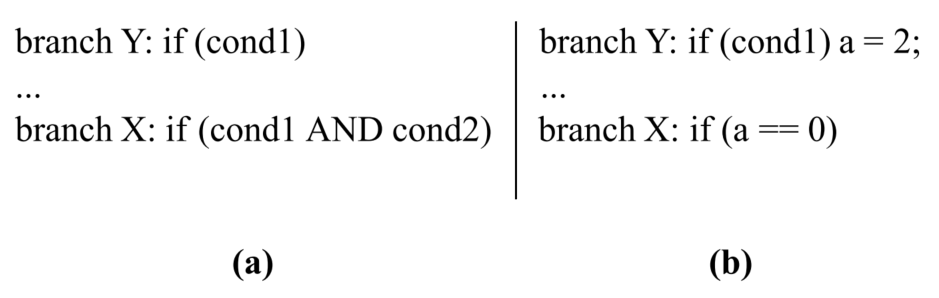
\includegraphics[width=0.5\linewidth]{assets/11/branch-direction-correlation.png}
  \caption{条件分支指令间的方向相关}
  \label{fig:branch-direction-correlation}
\end{figure}

除了方向相关外，不同的条件分支指令之间也存在路径相关。如图 \ref{fig:branch-path-correlation} 所示，假设
分支 X 不被分支 X、Z、V 控制（即无论分支 X、Z、V 跳转方向如何，分支 X 一定会
被执行），如果分支 V 被执行了，那么意味着分支 Y 和分支 Z 均未执行，因此无论分支
V 是否跳转，分支 X 一定执行跳转。分支 V 与分支 X 之间存在路径相关。

\begin{figure}[htbp]
  \centering
  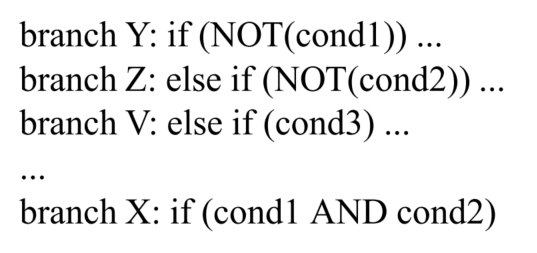
\includegraphics[width=0.5\linewidth]{assets/11/branch-path-correlation.png}
  \caption{条件分支指令间的路径相关}
  \label{fig:branch-path-correlation}
\end{figure}

针对条件分支指令存在的可预测性，历史上研究者们提出了很多种方法来预测条件分支指令的方向，本书将在 11.4.3 节中对此进行介绍。

由于无条件间接跳转类指令的跳转目标地址来自寄存器，直到执行时处理器才可以得知这类指令的跳转目标地址，因此有必要对此类指令的跳转目标地址进行预测。
一类容易预测的无条件间接跳转类指令是函数返回指令。由于函数调用与函数返回指令成对出现，且由于 ABI 的规定，函数调用与返回指令很容易被识别，因此可以用
一种特殊的存储结构存储函数的返回地址，这种结构一般被称为返回地址栈（Return Address Stack，RAS），本书将在 11.4.4 节对此进行介绍。

\subsection{分支目标缓冲}\label{sec:11-advanced-cpu-019}

分支目标缓冲（BTB）是分支预测器的核心，分支预测器中的其它组件都要依赖
BTB 提供的信息做出预测。由于 BTB 缓存分支指令的跳转地址及类型等信息，因此其
组织结构与高速缓存类似，可以实现为全相联、直接映射或多路组相联。在查询 BTB
时使用 PC 值的一部分作为索引（index）来寻址 BTB，PC 值的高位作为标签（tag）与
从 BTB 读出的表项中的标签域进行匹配生成命中或缺失信号。

\subsection{方向预测器}\label{sec:11-advanced-cpu-020}

方向预测器负责对条件分支指令的跳转方向做出预测。条件分支类指令往往是程序
执行过程中被执行次数最多的分支指令类型，其动态指令数往往远高于无条件跳转类指
令，因此对条件分支指令跳转方向的预测准确率会基本决定总体的分支预测准确率，从
而影响处理器性能。研究者们针对条件分支指令的方向预测进行了大量的研究。本节
将首先介绍最简单的方向预测器 BiModal 预测器，随后以 GShare 预测器为例引入全局分支历史的概念，最后介绍全局分
支历史的推测更新方式。

\subsubsection{BiModal 预测器}\label{sec:11-advanced-cpu-021}

BiModal 预测器是一种经典的条件分支方向预测器，它对条件分支指令的跳转倾向
进行预测。如图 \ref{fig:BiModal} 所示，它的主体是一个由一系列两位饱和计数器组成的模式历史
表（Pattern History Table，PHT），使用 PC 的低位索引 PHT，读出表项的最高位作为预
测的跳转方向，最高位为 1 表示跳转，为 0 表示不跳转。在更新时使用条件分支指令的
PC 索引 PHT，并根据指令的正确跳转方向更新对应的两位饱和计数器，当预测正确时
对计数器非上溢加一（即如果计数器值为 3 则不再加），当预测错误时对计数器非下溢
减一（即如果计数器值为 0 则不再减）。

\begin{figure}[htbp]
  \centering
  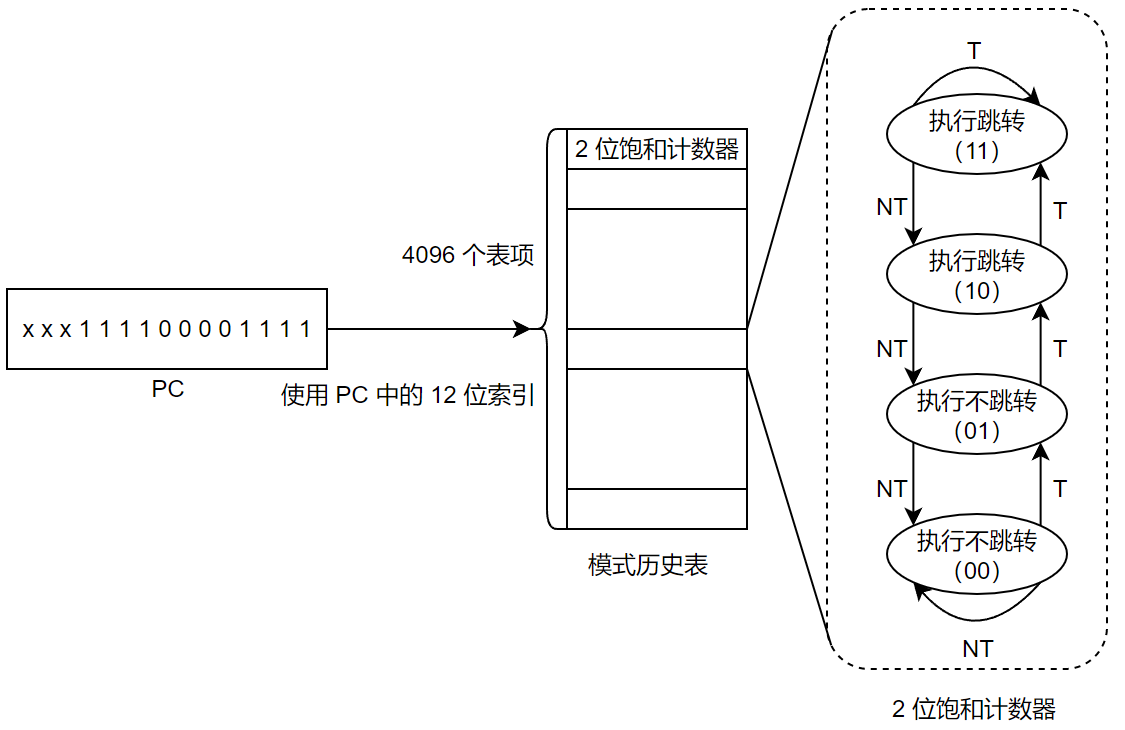
\includegraphics[width=0.5\linewidth]{assets/11/BiModal.png}
  \caption{BiModal 预测器}
  \label{fig:BiModal}
\end{figure}

BiModal 预测器仅考虑了分支指令自身跳转方向的倾向性，而忽略了分支指令自身
及不同分支指令跳转方向之间的许多潜在规律。因此其预测准确率不高，
BiModal 预测器在 SPEC CPU 1989 基准测试集上的平均预测准确率最高不到 94\%。

\subsubsection{使用全局模式历史------以 GShare 预测器为例}\label{sec:11-advanced-cpu-022}

可以使用一个全局的模式历史寄存器（Pattern History Register，PHR）来记录指令
流中条件分支指令的跳转方向。每执行一条条件分支指令，PHR 左移一位，并将最低位
置为该条条件分支的跳转方向（如跳转为 1，不跳转为 0）。如图 \ref{fig:GShare} 所示，GShare 预测
器将分支指令的 PC 中某些位（一般为 PC 的低位，也可以是 PC 哈希后的值）与 PHR
按位异或后得到的结果作为索引来选择 PHT 中的一个饱和计数器，然后将这个计数器
的最高位作为预测的跳转方向（如为 1 则跳转，否则不跳转）。更新时也通过同样的索
引方式索引到同一个饱和计数器进行更新。GShare 预测器的这种预测方式将不同全局
模式历史下的同一条分支指令的预测划分给了不同的饱和计数器，从而使得 GShare 预
测器可以捕捉单条分支指令自身跳转方向的规律性，以及不同条件分支指令之间的方向
相关性。

\begin{figure}[htbp]
  \centering
  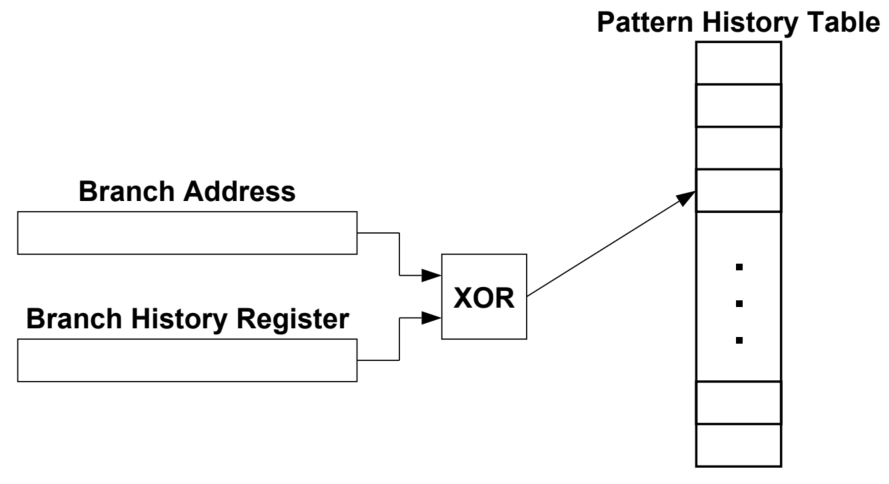
\includegraphics[width=0.5\linewidth]{assets/11/GShare.png}
  \caption{GShare 预测器}
  \label{fig:GShare}
\end{figure}

然而，GShare 预测器所需要的 PHT 表项个数与 PHR 的位宽呈指数关系，设 PHT
表项个数为 x，PHR 位宽为 y，则 \$ x = 2\^{}y \$。因此 PHR 每增加一位，PHT 表项数量需要增
加一倍。因此由于预测器面积与访问时间的限制，GShare 预测器无法使用较长的全局
模式历史，这限制了 GShare 预测器的准确率。

为了可以使用更长的全局模式历史，研究者们提出了很多预测器结构，如基于神经
网络的感知机预测器，基于 PPM 压缩算法的 PPM-like 预测器，使用呈几何级数长
度的全局分支历史的 O-GEHL 预测器，以及最终的集大成者 TAGE 预测器。目前
几乎所有的学术研究和商业高性能处理器都使用 TAGE 或者 TAGE 的变种作为提供高
准确率预测结果的条件分支预测器。

\subsubsection{推测更新全局模式历史}\label{sec:11-advanced-cpu-023}

在现代高性能处理器中的流水线中往往会同时存在上百条待执行的指令，而程序中
分支指令是较为密集的，通常平均每 5 到 10 条指令中就有一条是分支指令。因此如
果等待条件分支指令执行后，再根据执行结果更新全局模式历史寄存器，会导致在条件
分支指令被取进处理器流水线到被执行的这一段时间内，对在它后面被取进流水线的条
件分支指令进行跳转方向的预测时使用的不是最新的全局模式历史，从而极大的影响条
件分支预测器的预测准确率。

为了解决这一问题，目前普遍采用的做法是推测更新全局模式历史：当分支预测器
给出条件分支指令的方向预测结果后，立刻更新全局模式历史寄存器，从而保证每一次
预测都使用的是最新的全局模式历史。相应的，当检测到分支误预测时，需要对推测更
新的全局模式历史进行恢复。

\subsubsection{返回地址栈}\label{sec:11-advanced-cpu-024}

返回地址栈（Return Address Stack, RAS）是现代处理器中用于优化函数调用与返回性能的一种硬件结构。
它主要用于预测函数返回指令的目标地址，从而减少函数调用与返回过程中可能造成的流水线停顿。

在程序执行过程中，函数调用是一个非常常见的操作。当处理器执行函数调用指令时，
它会跳转到被调用函数的地址，并在函数执行完毕后返回调用点继续执行。
为了能够正确地返回调用点，处理器需要保存函数调用前的返回地址（即调用点的下一条指令的地址）。
然而，在深度流水线或多发射处理器中，等待函数返回指令的执行结果可能导致性能下降。
RAS 通过预测返回地址来缓解这一问题。RAS 的功能由函数调用时的地址存储、函数返回时的地址预测与
验证更新三部分组成：

\begin{itemize}
\tightlist
\item
  函数调用时的地址存储：当处理器遇到函数调用指令（如 BL/JIRL 指令）时，它会将返回地址（即函数调用后的指令地址）压入 RAS 中，同时跳转到被调用函数的地址。
\item
  函数返回时的地址预测：当处理器遇到函数返回指令（如 JIRL 指令）时，它会从 RAS 中弹出最顶端的地址，并预测这个地址是正确的返回地址。处理器然后使用这个预测地址来继续取指令并执行。
\item
  验证与更新：如果处理器预测的返回地址正确，执行继续而无需额外操作。如果预测错误，处理器需要回滚错误执行的指令，并将正确的返回地址更新到 RAS 中。
\end{itemize}

% !TeX root = ../main.tex
% 原始章节：12-fpga-verification.Rmd

\chapter{FPGA上板验证}\label{chap:12-fpga-verification}

\section{基于百芯计划实验箱的基本功能验证}\label{sec:12-fpga-verification-001}

\subsection{实验箱介绍}\label{sec:12-fpga-verification-002}

龙芯``百芯计划''处理器芯片全流程设计，自底向下包括：IP核结构设计、SoC芯片结构设计、芯片后端物理设计、芯片流片封装、硅后系统验证、应用系统开发。各参与高校可根据自身需求参与部分或全部流程的设计。其中IP核结构设计部分，龙芯将会提供参考处理器核设计，处理器核的验证环境与测试用例，合作高校可以进行处理核结构设计与验证或加速器结构设计与验证等。SoC芯片结构设计部分，龙芯将会提供成套外围IP的代码，各接口的驱动程序，专用FPGA设计实验平台，合作高校可以在SoC中IP集成与系统级验证（FPGA）等。芯片后端物理设计部分，龙芯将会提供物理设计参考设计flow，核外部分的GDS，合作高校可以进行全芯片物理设计或IP核物理设计等。硅后系统验证部分，龙芯将会提供开发板设计参考，合作高校可以在开发板对芯片各功能进行系统调试与验证等。应用系统开发部分，合作高校可以基于芯片研制具体问题的解决方案等。

板卡在原有基础上去掉板载NAND颗粒，改成TF卡槽，方便大容量存储拓展；增加SDRAM颗粒，方便学生使用SDRAM方案进行设计，容量增加到2Gb（删除原有的SRAM）；USB接口方案进行更换，接口拓展为4个，增加了更多外设的兼容；现有LCD屏更换为智能串口HMI屏，便于根据需求进行屏幕的个性化设计；增加SPI接口的引出。板卡可以满足百芯计划所需的外设需求，兼容原有的数字逻辑、体系结构、组成原理实验的硬件接口。板载系统资源如图\ref{fig:baixin-arch}所示。

\begin{figure}[htbp]
  \centering
  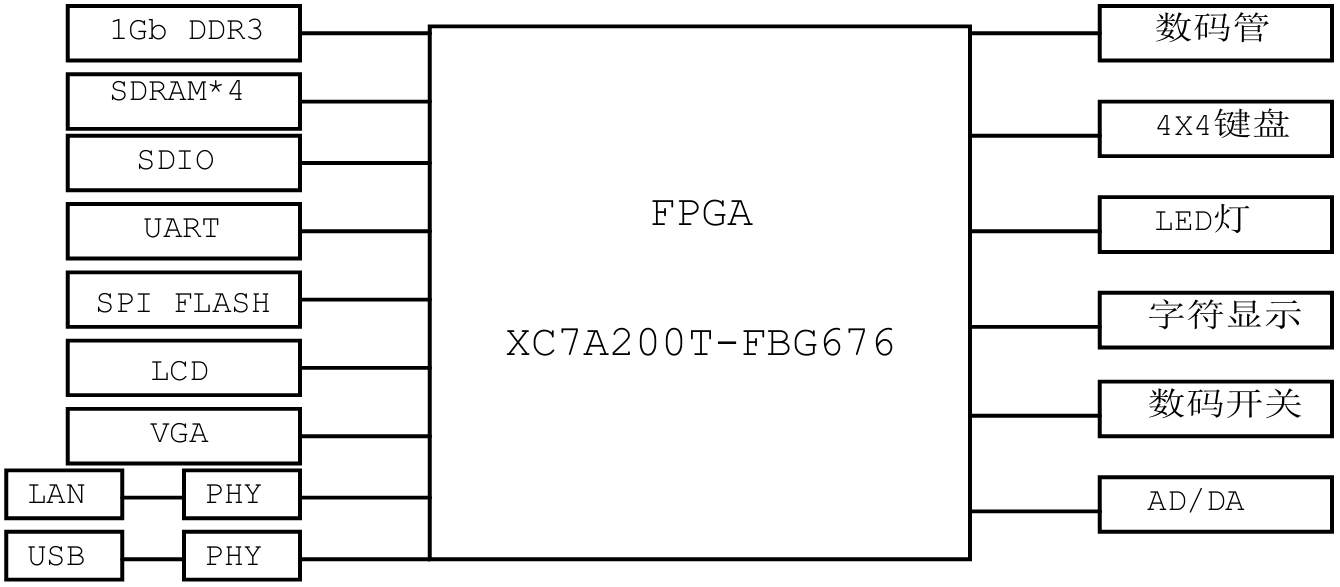
\includegraphics[width=0.75\linewidth]{assets/12/baixin_arch.png}
  \caption{百芯开发板资源}
  \label{fig:baixin-arch}
\end{figure}

\subsection{系统验证 SoC 介绍}\label{sec:12-fpga-verification-003}

龙芯提供的百芯开发板 SoC 位于chplab工程下，相关目录如下

% 代码语言：text
\begin{CodeBlock}
.
├── chip              SoC顶层。
│　　└── soc_demo       SoC顶层代码实例。
│　　　　　├── loongson    龙芯实验箱SoC顶层代码。
│　　　　　├── Baixin      百芯开发板SoC顶层代码。
│　　　　　└── sim       仿真SoC顶层代码
├── fpga              综合工程。
│　　├── loongson        龙芯实验箱综合工程。
│　　　　　├── 2019.2    对应Vivado 2019.2版本。
│　　　　　└── 2023.2    对应Vivado 2023.2版本。
│　　└── Baixin          百芯开发板综合工程。
├── IP                SoC IP。
│　　├── AMBA         总线 IP。
│　　├── APB_DEV       APB协议通信设备。
│　　　　　├── URT       UART设备控制器。
│　　　　　└── NAND     NAND设备控制器。
│　　├── AXI_DELAY_RAND  随机延迟注入。
│　　├── AXI_SRAM_BRIDGE  AXI协议 -> SRAM接口转换。
│　　├── BRIDGE        1x2桥接模块。
│　　├── DMA          DMA逻辑，用于设备作为master访问内存。
│　　├── SPI           SPI Flash设备控制器。
│　　├── MAC          MAC设备控制器。
│　　├── CONFREG       用于访问开发板上数码管、拨码开关等外设以及特殊寄存器。
│　　├── myCPU        处理器核逻辑。
│　　└── xilinx_ip        Vivado平台所创建的IP。
│　　　　　├── 2019.2    对应Vivado 2019.2版本。
│　　　　　└── 2023.2    对应Vivado 2023.2版本。
\end{CodeBlock}

SoC设备及地址空间划分如下：

\begin{longtable}[]{@{}
  >{\raggedright\arraybackslash}p{(\linewidth - 6\tabcolsep) * \real{0.3710}}
  >{\raggedright\arraybackslash}p{(\linewidth - 6\tabcolsep) * \real{0.0645}}
  >{\raggedright\arraybackslash}p{(\linewidth - 6\tabcolsep) * \real{0.3710}}
  >{\raggedright\arraybackslash}p{(\linewidth - 6\tabcolsep) * \real{0.1935}}@{}}
\toprule\noalign{}
\begin{minipage}[b]{\linewidth}\raggedright
地址范围
\end{minipage} & \begin{minipage}[b]{\linewidth}\raggedright
模块
\end{minipage} & \begin{minipage}[b]{\linewidth}\raggedright
描述
\end{minipage} & \begin{minipage}[b]{\linewidth}\raggedright
空间大小
\end{minipage} \\
\midrule\noalign{}
\endhead
\bottomrule\noalign{}
\endlastfoot
0x1C000000 - 0x1C0FFFFF & SPI & SPI 控制器（boot rom） & 1 MB \\
0x1FE80000 - 0x1FE8FFFF & SPI & SPI 控制器 & 64 KB \\
0x1FE00000 - 0x1FE0FFFF & APB & APB\_DEV: UART & 64 KB \\
0x1FE70000 - 0x1FE7FFFF & APB & APB\_DEV: NAND（未使用） & 64 KB \\
0x1FD00000 - 0x1FD0FFFF & CONF & 配置寄存器及GPIO & 64 KB \\
0x1FF00000 - 0x1FF0FFFF & MAC & MAC 控制器 & 64 KB \\
其他 & DDR3 & DDR3 内存 & 依赖具体实现 \\
\end{longtable}

\subsubsection{内核启动的方法}\label{sec:12-fpga-verification-004}

本文以内核启动为例简单介绍一下SoC代码整体的使用流程。

内核启动需要依次完成以下步骤：

\begin{itemize}
\tightlist
\item
  烧写 PMON 文件(\href{https://gitee.com/chenzes/chiplab-tools/releases/download/pmon/gzrom.bin}{gzrom.bin})或 u-boot文件(\href{https://gitee.com/llh730/la32r-uboot/releases}{uboot.bin})到可插拔 SPI flash 上。
\item
  生成并加载 bit 流文件。
\item
  运行 PMON / u-boot。
\item
  搭建 tftp 服务器 Load 内核(\href{https://gitee.com/loongson-edu/la32r-Linux/releases}{vmlinux})。
\item
  启动内核。
\end{itemize}

\textbf{1. 烧写PMON / u-boot}

烧录方面我们推荐使用\href{https://detail.tmall.com/item.htm?spm=a21n57.1.item.2.21e3523cc9elHp\&priceTId=2147bfb717231061625906771e52e0\&utparam=\%7B\%22aplus_abtest\%22\%3A\%22abee490f5aa02657b98af3e8efcc7a9b\%22\%7D\&id=807896685118\&ns=1\&abbucket=10\&xxc=taobaoSearch\&skuId=5659871783574\&pisk=fR8ttPGMuvDMFZnD5Cihow64wxGnEFdZIdR7otXgcpppG94m_NmVkKBp3OjG5O4AkIp2nKdq_s6XhKBDjD0k_C7VlY4xr4AwYwZe1dBbl9Gfa_rjW2mn1C7VlxF3l00J_LhWJmDAcXQCMsZ1lG_bR66FMsw6hOsQd_CPlt9flXQCgsXb5O_bOJ1jCDcF3vXuknOCXJ97-Sz0oeCI3TOTfrCHR1UCeCBKFV8LzGBW19UjE5hM5tBePvmpTLx6I6JxyvQW4pLAVZ3TU1KBww6GPVFNFFfvZnd-e-fefdLCDecqbBLABgT1vqhlRNCXhiKEezfOSHIJWhl4dC9lB3_wi7HM9gKd46sQMl_MqQYVVFgTU9jPMpIkXYU9Fgl6rUEjq8XRilGK9orVf6jlSZz6mdUr36BotGZ40MeO9TcK9orVf65dEX4_0oSLB}{CH341A编程器}烧写 PMON 文件(\href{https://gitee.com/chenzes/chiplab-tools/releases/download/pmon/gzrom.bin}{gzrom.bin})或 u-boot文件(\href{https://gitee.com/llh730/la32r-uboot/releases}{uboot.bin})到开发板搭载的可插拔 SPI flash 上。商家提供的资料比较全面，上位机软件支持图形化界面，使用简单。

\textbf{2. 下载bit流文件}

打开\texttt{chiplab/fpga/Baixin/system\_run/system\_run.xpr}工程综合并生成 bit 流。将开发板与主机间的下载线连接好，开发板上电，使用 Vavidao 工具里的 Open Hardware Manager 下载 bit 文件到开发板上。

\textbf{3. 运行PMON / u-boot}

上述烧写的 PMON / u-boot 运行在下载的 SoC 上，需要使用串口展示运行信息。 将开发板与主机间的串口线连接好，打开串口软件，波特率设置为 115200。

Windows下可以使用免安装的\href{https://gitee.com/chenzes/chiplab-tools/releases/download/chiplab-tools/SecureCRTPortable.zip}{SecureCRTPortable串口软件}。 先使用 USB 转串口和串口连接线将电脑和开发板相连。
双击程序打开，第一次启动界面如下图\ref{fig:secure-one}所示：

\begin{figure}[htbp]
  \centering
  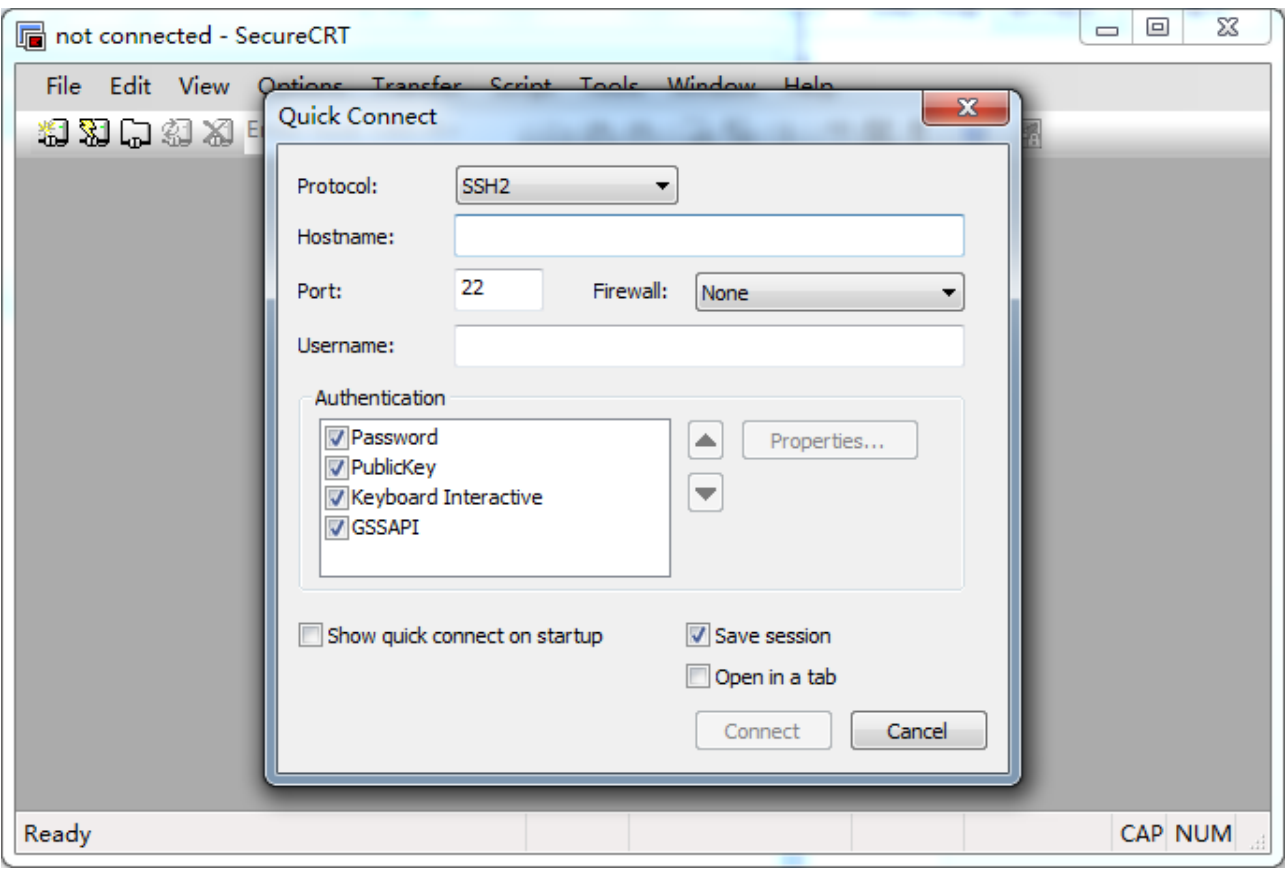
\includegraphics[width=0.75\linewidth]{assets/12/secure_one.png}
  \caption{启动界面}
  \label{fig:secure-one}
\end{figure}

第一行 Protocol 下拉选择 Serial，如下图\ref{fig:secure-two}所示：

\begin{figure}[htbp]
  \centering
  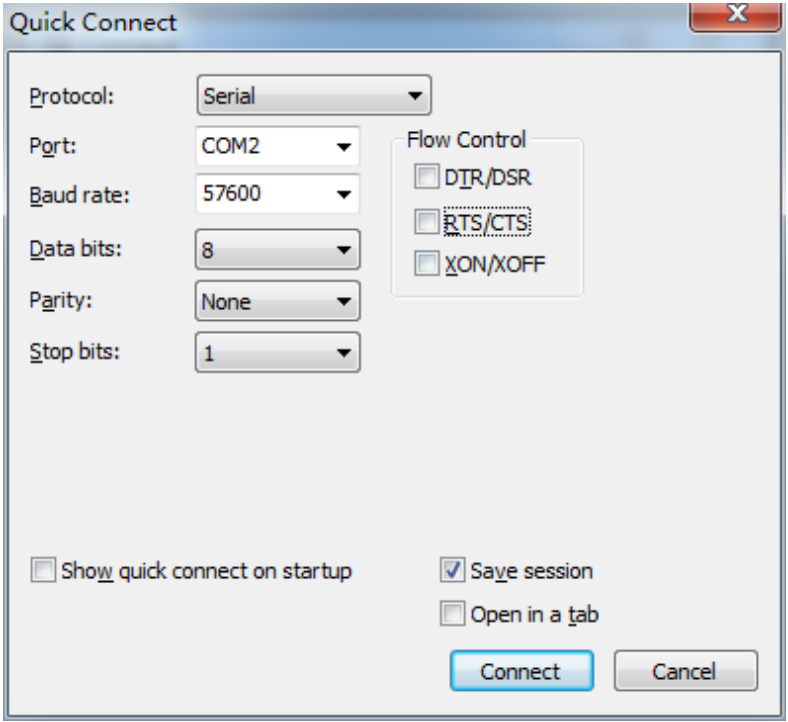
\includegraphics[width=0.75\linewidth]{assets/12/secure_two.png}
  \caption{选择串口}
  \label{fig:secure-two}
\end{figure}

其中 Baud rate 为选择波特率，需根据开发板上串口控制器的初始化代码中设置的波特率进行选择(对于本次校验设备，波特率需选择 115200)。右侧 Flow Control 全不选。Port 的选择需根据 Windows 电脑上的端口进行选择，可以右键电脑选择设备管理器进入设备管理器查看，如下图\ref{fig:secure-three}所示：

\begin{figure}[htbp]
  \centering
  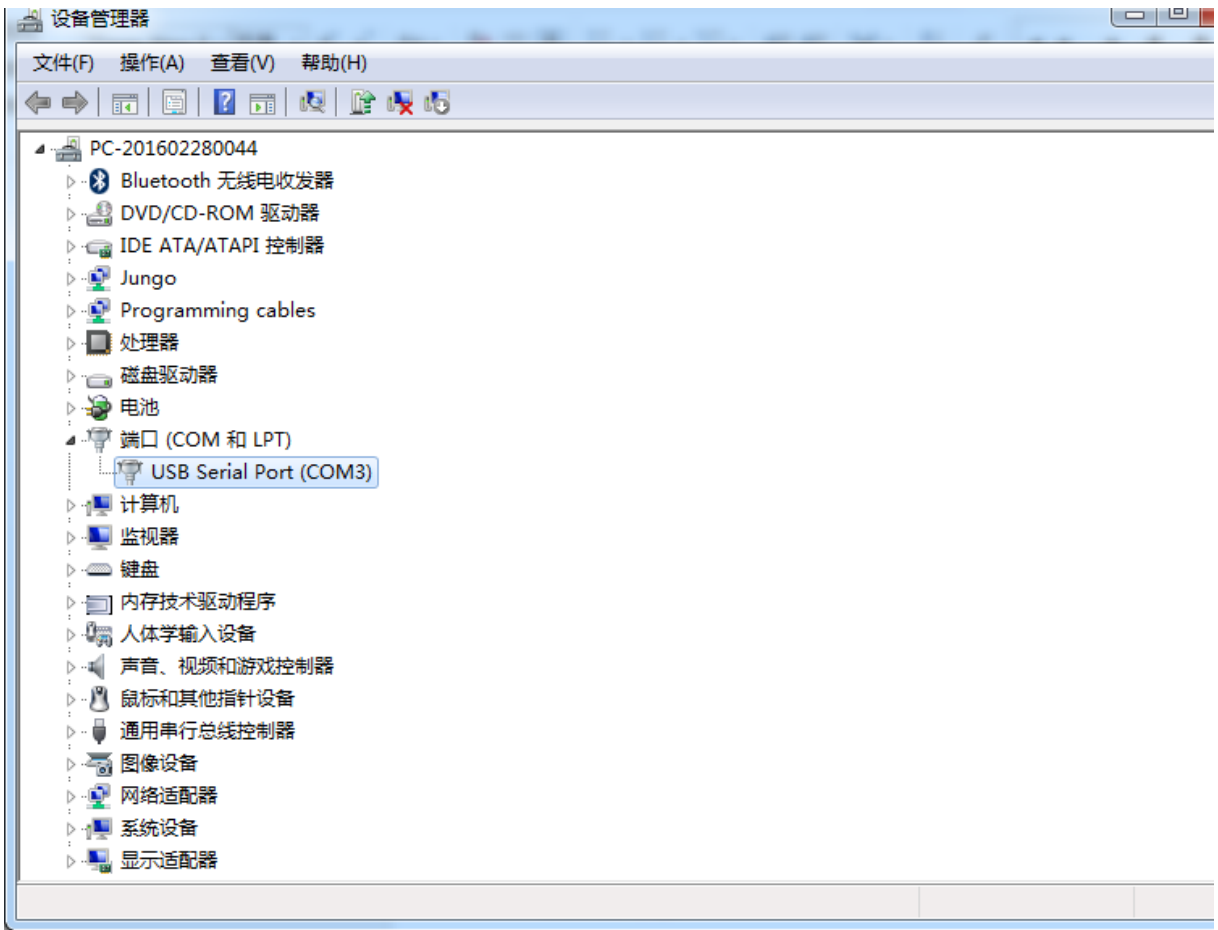
\includegraphics[width=0.75\linewidth]{assets/12/secure_three.png}
  \caption{配置串口}
  \label{fig:secure-three}
\end{figure}

配置好串口后，点击 connect，即可进入串口界面，在波特率设置正确的情况下，可以通过串口与开发板进行交互，如下图\ref{fig:secure-four}所示：

\begin{figure}[htbp]
  \centering
  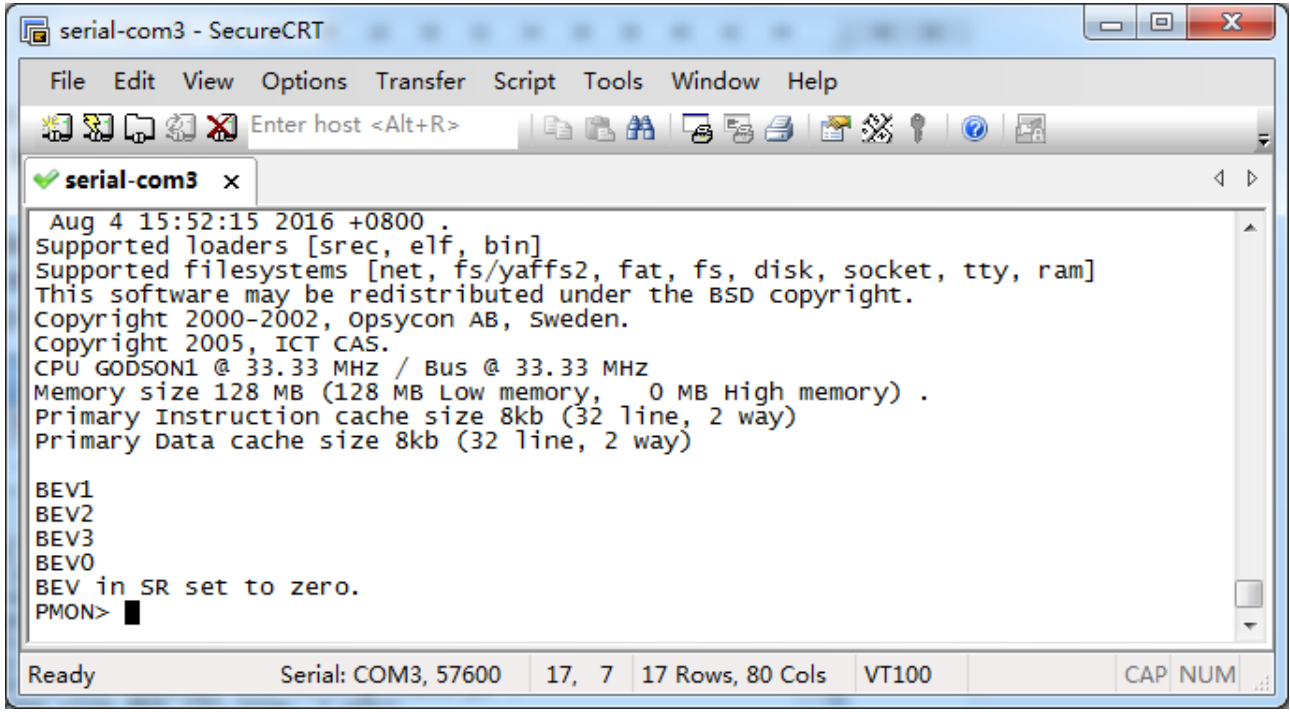
\includegraphics[width=0.75\linewidth]{assets/12/secure_four.png}
  \caption{成功连接串口}
  \label{fig:secure-four}
\end{figure}

\textbf{4. PMNO网络加载并运行Linux}

连接上串口，打开串口软件，设置好波特率，则可以在串口窗口中看到 PMON 运行信息，运行成功后则会进入 PMON 提示符，此时可以输入 PMON 命令。

比如， SoC 中具有 MAC 控制器，PMON 中也有 MAC 驱动，则我们输入命令

% 代码语言：text
\begin{CodeBlock}
ifconfig dmfe0 10.90.50.44
\end{CodeBlock}

则可以给开发板上的网卡配置 IP 为 10.90.50.44（具体需配置的 IP 请查阅同网段的电脑 IP），假设同网段的电脑 IP 为 10.90.50.43,则可以继续输入命令

% 代码语言：text
\begin{CodeBlock}
ping 10.90.50.43
\end{CodeBlock}

用于查看网络是否成功接入。Linux 在 ping 网络是会一直发 ping 包，可以 \texttt{Ctrl+C} 取消 ping。运行结果如下：

% 代码语言：text
\begin{CodeBlock}
PMON> ifconfig dmfe0 10.90.50.44
rx ring 70acee0
tx ring 70acf60
DE4X5_BMR= fe000000
DE4X5_TPD= 0
DE4X5_RRBA= 70acee0
DE4X5_TRBA= 70acf60
DE4X5_STS= f0660004
DE4X5_OMR= 32002242
TX error status2 = 0x00000000
After setup
DE4X5_BMR= fe000000
DE4X5_TPD= 0
DE4X5_RRBA= 70acee0
DE4X5_TRBA= 70acf60
DE4X5_STS= f0660004
DE4X5_OMR= 32002242
PMON> ping 10.90.50.43
PING 10.90.50.43 (10.90.50.43): 56 data bytes
64 bytes from 10.90.50.43: icmp_seq=0 ttl=64 time=3.708 ms
64 bytes from 10.90.50.43: icmp_seq=1 ttl=64 time=2.331 ms
64 bytes from 10.90.50.43: icmp_seq=2 ttl=64 time=2.235 ms

--- 10.90.50.43 ping statistics ---
3 packets transmitted, 3 packets received, 0% packet loss
round-trip min/avg/max = 2.235/2.750/3.708 ms
PMON>
\end{CodeBlock}

由于运行 linux 时，最初的内核需要使用网口 load 进入内存执行，因而需要先搭建 Tftp 服务器。
具体方法参见\href{https://gitee.com/chenzes/chiplab-tools/releases/download/chiplab-tools/tftp.zip}{tftp下载地址}。
目前运行 Linux 的方法是，先运行 PMON，随后通过网口 load Linux 内核进入 FPGA 上的 DDR3 内存上。在load内核前，需要通过以下命令裁剪掉内核二进制文件中的符号信息。

% 代码语言：text
\begin{CodeBlock}
loongarch32r-linux-gnusf-strip vmlinux
\end{CodeBlock}

load 命令为

% 代码语言：text
\begin{CodeBlock}
load tftp://10.90.50.43/vmlinux
\end{CodeBlock}

其中 10.90.50.43 为搭建的 tftp 服务器的 IP。
串口的波特率为 115200。
具体过程如下：
启动 PMON 后，输入命令

% 代码语言：text
\begin{CodeBlock}
ifconfig dmfe0 10.90.50.44
\end{CodeBlock}

给开发板上的网卡配置 IP 为 10.90.50.44（具体需 配置的 IP 请查阅同网段的电脑 IP），假设同网段的电脑 IP 为 10.90.50.43, 则可以继续输入命令

% 代码语言：text
\begin{CodeBlock}
ping 10.90.50.43
\end{CodeBlock}

用于查看网络是否成功接入。
网络配置好了，需要通过网络下载 Linux 内核，需要先搭建好 tftp 服务器，假设搭建的 tftp 服务器 IP 为 10.90.50.43，将要下载 Linux 内核放到 tftp 服务器的根目录下，输入命令

% 代码语言：text
\begin{CodeBlock}
load tftp://10.90.50.43/vmlinux
\end{CodeBlock}

即可 load 内核进入 FPGA 上的内存。

% 代码语言：text
\begin{CodeBlock}
PMON> load tftp://10.90.50.43/vmlinux
Loading file: tftp://10.90.50.43/vmlinux (elf)
0x80200000/5350380 + 0x8071a3ec/169220(z) + 6926 syms\
Entry address is 802041f0
PMON> g console=ttyS0,115200 rdinit=sbin/init
\end{CodeBlock}

上表中显示 load 成功了，输入命令

% 代码语言：text
\begin{CodeBlock}
g console=ttyS0,baudrate rdinit=sbin/init
\end{CodeBlock}

即可运行该内核，命令中 baudrate 需为数字，即为串口控制器设置的波特率，设置不对时，串口显示字符为乱码。Linux 内核运行时波特率为 115200。
当运行 Linux 内核成功后会出现\texttt{/\ \#}提示符，可以使用常用的 Linux 命令。

\textbf{4. U-Boot网络加载并运行Linux}

连接上串口，打开串口软件，设置好波特率，则可以在串口窗口中看到 u-boot 运行信息，运行成功后则会进入 u-boot 提示符，此时可以输入 u-boot 命令。

在u-boot中使用\texttt{print}命令可以查看当前的环境配置。

使用命令（\textbf{请使用自己的IP}）

% 代码语言：text
\begin{CodeBlock}
setenv ipaddr 10.90.50.44
setenv serverip 10.90.50.43
\end{CodeBlock}

可以配置u-boot和服务器（自己电脑）的使用的ip（两者需在同一子网下，配置的具体IP需查看自己本机IP），u-boot中通过命令

% 代码语言：text
\begin{CodeBlock}
ping 10.90.50.43
\end{CodeBlock}

可以查看与服务器是否建立了连接。

完成了网络配置，就可以使用uboot加载内核，使用命令

% 代码语言：text
\begin{CodeBlock}
setenv bootcmd console=ttyS0,115200 rdinit=/init
\end{CodeBlock}

可以配置内核的启动参数。 通过命令

% 代码语言：text
\begin{CodeBlock}
tftpboot 0xa3000000 vmlinux
\end{CodeBlock}

可以将内核加载到 \texttt{0xa300\_0000} 开始的地址上，该地址并不是\texttt{readelf}显示的\texttt{entry}的入口地址。uboot会先把镜像加载到一段无数据的地址，运行时再根据elf段的信息加载到对应的位置上。

最后，使用命令

% 代码语言：text
\begin{CodeBlock}
bootelf 0xa3000000 bootcmd
\end{CodeBlock}

即可成功运行linux内核！

\section{设计包含各类外设的测试板}\label{sec:12-fpga-verification-005}

如果现有的开发板资源不满足我们的开发需求，我们可自行设计验证板（包括FPGA测试板和回片测试板）、板载集成支持各类外设配套的控制器、转接口、IO调试等资源，以完整验证CPU功能、操作系统与应用程序验证演示。但是PCB电路设计相关知识和注意事项并不是本文关注的重点，这里仅对一些常见且必要的设备做简单介绍。在实践流程文档中，我们将以LainBoard为例，介绍测试板的设计。

\subsection{DRAM控制器}\label{sec:12-fpga-verification-006}

DRAM内存是整个SoC的主存储器，在整个SoC中占有最重要的地位，其容量决定了CPU处理大量数据的能力大小，而其速率决定了CPU处理数据的快慢。同时，如果DRAM控制器不工作，则在选定SDRAM内存是1990年代的技术，速度较慢，但其接口简单，没有复杂的时序要求，且芯片廉价易购买。SDRAM具有由时钟驱动的同步传输接口，只需要使用简单的IOPAD及开源的控制器IP核就可驱动，而如果使用DDR内存，则需要增加Interface PHY IP核和控制器，增加设计的复杂程度。一般考虑项目的实际情况，最适宜的内存类型就是SDRAM内存。

\subsection{SPI Flash控制器}\label{sec:12-fpga-verification-007}

SPI Flash控制器通过SPI总线接口连接到芯片外部的SPI Flash总线，对内具有AXI接口，将AXI接口上的访存请求翻译为SPI Flash控制指令，然后从Flash存储芯片中读出数据并在AXI接口上返回。CPU核心启动时的PC地址对应SPI Flash存储区域，开机时CPU即可通过直接访存的形式读取Bootloader代码并执行。使用SPI Flash存放启动代码的好处是可以使启动代码在芯片设计结束后随时可修改，避免在芯片内部使用ROM固化的代码中存在Bug的情况。SPI Flash控制器也兼具SPI控制器的作用，可以连接SPI LCD显示屏等外设，并进行高速双向通信。对应的，测试板上可搭载Flash芯片或引出SPI接口。

\subsection{以太网控制器}\label{sec:12-fpga-verification-008}

网络通信是计算机系统的重要能力。以太网接口控制器分为两部分：MAC和PHY，前者为逻辑控制器，很容易放进芯片中；后者为物理层接口，一般需要模拟电路来实现，两者之前采用MII或RMII接口相连{[}27{]}。在芯片中具有AXI接口的以太网控制器，该控制器支持10/100Mbps的通信速率，与外部以MII总线相连，并外接了MII转RMII转换器，对外暴露RMII接口。

以太网控制器分为总线、网络两个时钟域，总线时钟域负责与CPU进行通信，网络时钟域负责与MII接口进行通信，两个模块之间通过CDC同步器进行沟通。以太网控制器模块内具有四个双端口SRAM存储器，每个存储器的两个端口分别连接到两个时钟域。在发送数据包时，首先在总线时钟域侧由CPU将数据写入SRAM，然后网络时钟域侧的逻辑将SRAM内容搬运到MII接口；接收数据包时，在网络时钟域侧从MII接口将数据包内容搬运到SRAM，再由CPU向总线时钟域侧的逻辑读取。

MII是控制器与PHY的中间数字接口，并不是最终连接以太网的接口。芯片要与实际的以太网接口相连，还需要PHY芯片将数字接口适配以太网接口的物理定义。

\subsection{SD卡控制器}\label{sec:12-fpga-verification-009}

现代操作系统通常需要磁盘的支持，用于存放程序、资源文件、用户文件等。主流计算机磁盘的接口有IDE、SATA、NVMe等，但这些接口（特别是后两者）都较为复杂，在短时间内集成进本芯片是不现实的。SD卡作为近年来新兴的存储设备，具有简单的协议和接口，且容量大、价格低廉、容易购买，适合作为测试板的存储设备使用。

\subsection{I2C控制器}\label{sec:12-fpga-verification-010}

I2C（全称Inter-Integrated Circuit）是Philips公司于1982年提出的一种通讯总线，使用两条线就可以连接多个外设，使PCB设计变得更加简单方便。I2C总线通常用于连接低速外设，如各种传感器。

\subsection{UART控制器}\label{sec:12-fpga-verification-011}

UART控制器使芯片可以通过UART协议（串口）与外部进行通信。龙芯教育提供了一个标准的16550 UART控制器，挂接到APB总线下。UART控制器中有FIFO功能，CPU可以一次性写入多组数据，加快通信速率。

\subsection{USB控制器}\label{sec:12-fpga-verification-012}

USB（通用串行总线）是一种广泛使用的设备接口，用于连接电脑和其他电子设备。它允许设备之间的数据传输，并可以为连接的设备供电。一般来说在SoC中会继承支持ULPI接口的USB控制器，而开发板则需要搭载USB PHY芯片以支持USB通信。

\subsection{小结}\label{sec:12-fpga-verification-013}

总的来说我们的测试板一般需要搭载如下设备：

\begin{enumerate}
\def\labelenumi{\arabic{enumi}.}
\tightlist
\item
  电源控制芯片
\item
  SDRAM内存芯片
\item
  Flash闪存芯片
\item
  以太网PHY芯片和RJ45网口
\item
  USB PHY芯片及USB母座
\item
  SD卡插槽
\item
  SPI、GPIO、I2C等信号接口排母
\item
  按需求添加的其他设备
\end{enumerate}

% !TeX root = ../main.tex
% 原始章节：13-opration-system.Rmd

\chapter{操作系统移植}\label{chap:13-operating-system}

\section{运行操作系统所需要的支持}\label{sec:13-operating-system-001}

操作系统是直接运行在硬件上的一类特殊软件，可以进一步向用户软件提供支持服务和维护。

本文语境下的操作系统，指具有抢占式调度且支持页式内存管理的常见通用操作系统。
当我们的处理器对MMU、中断异常、时钟、MMIO 等硬件机制提供足够支持后，就具备了运行操作系统的基本硬件条件。之后需要做的就是完成操作系统对处理器的适配。
操作系统对处理器的适配具体来说，也就是对上面的几个硬件机制的适配融合。

操作系统软件借助 MMU 和异常完成页式内存管理，借助时钟和中断完成抢占式调度支持，借助 MMIO 实现交互和对更多硬件的控制。
操作系统移植，实际就是将操作系统的这些机能，具体实现到对应体系结构的硬件机制上。以下我们以教学操作系统 MOS 的移植为例，展示移植的具体过程。之后以 Linux 为例，介绍对驱动进行适配的板级移植。

\section{MOS 移植流程}\label{sec:13-operating-system-002}

\subsubsection{1. 为新的体系结构定义头文件定义}\label{sec:13-operating-system-003}

为新的体系结构准备体系结构相关的头文件。这些头文件通常包含通用寄存器定义，控制状态寄存器定义，页表属性定义，部分内联汇编函数定义等。

如下文件，定义了 LoongArch32 指令集中的所有通用寄存器别名以及控制状态寄存器。

% 代码语言：BookC
\begin{CodeBlock}[language=BookC]
#ifndef _SYS_REGDEF_H
#define _SYS_REGDEF_H

#define zero $r0
#define ra $r1
#define tp $r2
#define sp $r3
#define a0 $r4
#define a1 $r5
#define a2 $r6
#define a3 $r7
#define a4 $r8
#define a5 $r9
#define a6 $r10
#define a7 $r11
#define v0 $r10 // r4
#define v1 $r11 // r5
#define t0 $r12
#define t1 $r13
#define t2 $r14
#define t3 $r15
#define t4 $r16
#define t5 $r17
#define t6 $r18
#define t7 $r19
#define t8 $r20
#define x $r21
#define fp $r22
#define s0 $r23
#define s1 $r24
#define s2 $r25
#define s3 $r26
#define s4 $r27
#define s5 $r28
#define s6 $r29
#define s7 $r30
#define s8 $r31

#define csr_crmd 0x0
#define csr_prmd 0x1
#define csr_euen 0x2
#define csr_ectl 0x4
#define csr_estat 0x5
#define csr_era 0x6
#define csr_badv 0x7
#define csr_eentry 0xc
#define csr_tlbidx 0x10
#define csr_tlbehi 0x11
#define csr_tlbelo0 0x12
#define csr_tlbelo1 0x13
#define csr_asid 0x18
#define csr_pgdl 0x19
#define csr_pgdh 0x1a
#define csr_pgd 0x1b
#define csr_cpuid 0x20
#define csr_save0 0x30
#define csr_save1 0x31
#define csr_save2 0x32
#define csr_save3 0x33
#define csr_tid 0x40
#define csr_tcfg 0x41
#define csr_tval 0x42
#define csr_ticlr 0x44
#define csr_llbctl 0x60
#define csr_tlbrentry 0x88
#define csr_dmw0 0x180
#define csr_dmw1 0x181

#define ESTAT_SWI0 0x0001
#define ESTAT_SWI1 0x0002
#define ESTAT_HWI0 0x0004
#define ESTAT_HWI1 0x0008
#define ESTAT_HWI2 0x0010
#define ESTAT_HWI3 0x0020
#define ESTAT_HWI4 0x0040
#define ESTAT_HWI5 0x0080
#define ESTAT_HWI6 0x0100
#define ESTAT_HWI7 0x0200
#define ESTAT_TI 0x0800
#define ESTAT_IPI 0x1000

#define ESTAT_ECODE 0x003f0000
#define ESTAT_ESUBCODE 0x7fc00000

#define CRMD_PLV 0x0003
#define CRMD_IE 0x0004
#define CRMD_DA 0x0008
#define CRMD_PG 0x0010
#define CRMD_DATF 0x0020
#define CRMD_DATM 0x0080

#define PRMD_PPLV 0x0003
#define PRMD_PIE 0x0004

#endif /* _SYS_REGDEF_H */
\end{CodeBlock}

如下文件定义了缓存行的相关控制内联汇编函数：

% 代码语言：BookC
\begin{CodeBlock}[language=BookC]
#ifndef __ASM_CACHEOPS_H
#define __ASM_CACHEOPS_H

#ifndef __ASSEMBLY__

static inline void la_cache(int op, const volatile void *addr)
{
    __asm__ __volatile__("cacop %0, %1" : : "i"(op), "R" (*(unsigned char *)(addr)));
}

#define MIPS32_WHICH_ICACHE                    0x0
#define MIPS32_FETCH_AND_LOCK                  0x7

#define ICACHE_LOAD_LOCK (MIPS32_WHICH_ICACHE | (MIPS32_FETCH_AND_LOCK << 2))

/* Prefetch and lock instructions into cache */
static inline void icache_lock(void *func, size_t len)
{
}
#endif /* !__ASSEMBLY__ */

#define Cache_I             0x00
#define Cache_D             0x01
#define Cache_V             0x02
#define Cache_S             0x03

#define INDEX_INVALIDATE        0x08
#define INDEX_WRITEBACK_INV     0x08
#define HIT_INVALIDATE          0x10
#define HIT_WRITEBACK_INV       0x10

#define INDEX_INVALIDATE_I      (Cache_I | INDEX_INVALIDATE)
#define INDEX_WRITEBACK_INV_D   (Cache_D | INDEX_WRITEBACK_INV)
#define HIT_INVALIDATE_I        (Cache_I | HIT_INVALIDATE)
#define HIT_INVALIDATE_D        (Cache_D | HIT_INVALIDATE)
#define HIT_WRITEBACK_INV_D     (Cache_D | HIT_WRITEBACK_INV)

#endif  /* __ASM_CACHEOPS_H */

\end{CodeBlock}

如下文件定义了内核态下的虚拟内存布局，及虚拟地址相关的宏定义：

% 代码语言：BookC
\begin{CodeBlock}[language=BookC]
#ifndef _MMU_H_
#define _MMU_H_

#include <error.h>

#define PMEMSIZE (56 * 1024 * 1024)

#define NASID 1024
#define PAGE_SIZE 4096
#define PTMAP PAGE_SIZE
#define PDMAP (4 * 1024 * 1024) // bytes mapped by a page directory entry
#define PGSHIFT 12
#define PDSHIFT 22 // log2(PDMAP)
#define PDX(va) ((((u_long)(va)) >> PDSHIFT) & 0x03FF)
#define PTX(va) ((((u_long)(va)) >> PGSHIFT) & 0x03FF)
#define PTE_ADDR(pte) (((u_long)(pte)) & ~0xFFF)
#define PTE_FLAGS(pte) (((u_long)(pte)) & 0xFFF)

// Page number field of an address
#define PPN(pa) (((u_long)(pa)) >> PGSHIFT)
#define VPN(va) (((u_long)(va)) >> PGSHIFT)

// Global bit. When the G bit in a TLB entry is set, that TLB entry will match solely on the VPN
// field, regardless of whether the TLB entry’s ASID field matches the value in EntryHi.
#define PTE_G (0x0001 << (6 + 4))

// Valid bit. If 0 any address matching this entry will cause a tlb miss exception (TLBL/TLBS).
#define PTE_V (0x0001 << (0 + 4))

// Dirty bit, but really a write-enable bit. 1 to allow writes, 0 and any store using this
// translation will cause a tlb mod exception (TLB Mod).
#define PTE_D (0x0001 << (1 + 4))

// Permission bit.
#define PTE_PLV (0x0003 << (2 + 4))

// Cacheable bit. 1 to make the access cacheable, 0 for uncacheable.
#define PTE_C (0x0001 << (4 + 4))

// Copy On Write. Reserved for software, used by fork.
#define PTE_COW 0x0001

// Shared memmory. Reserved for software, used by fork.
#define PTE_LIBRARY 0x0002

// Memory segments (32-bit kernel mode addresses)
#define KUSEG 0x00000000U
#define KSEG0 0x80000000U
#define KSEG1 0xA0000000U
#define KSEG2 0xC0000000U

/*
 * Part 2.  Our conventions.
 */

/*
 o     4G ----------->  +----------------------------+------------0x100000000
 o                      |       ...                  |  kseg2
 o      KSEG2    -----> +----------------------------+------------0xc000 0000
 o                      |          Devices           |  kseg1
 o      KSEG1    -----> +----------------------------+------------0xa000 0000
 o                      |      Invalid Memory        |   /|\
 o                      +----------------------------+----|-------Physical Memory Max
 o                      |       ...                  |  kseg0
 o      KSTACKTOP-----> +----------------------------+----|-------0x8040 0000-------end
 o                      |       Kernel Stack         |    | KSTKSIZE            /|\
 o                      +----------------------------+----|------                |
 o                      |       Kernel Text          |    |                    PDMAP
 o      KERNBASE -----> +----------------------------+----|-------0x8002 0000    |
 o                      |      Exception Entry       |   \|/                    \|/
 o      ULIM     -----> +----------------------------+------------0x8000 0000-------
 o                      |         User VPT           |     PDMAP                /|\
 o      UVPT     -----> +----------------------------+------------0x7fc0 0000    |
 o                      |           pages            |     PDMAP                 |
 o      UPAGES   -----> +----------------------------+------------0x7f80 0000    |
 o                      |           envs             |     PDMAP                 |
 o  UTOP,UENVS   -----> +----------------------------+------------0x7f40 0000    |
 o  UXSTACKTOP -/       |     user exception stack   |     PTMAP                 |
 o                      +----------------------------+------------0x7f3f f000    |
 o                      |                            |     PTMAP                 |
 o      USTACKTOP ----> +----------------------------+------------0x7f3f e000    |
 o                      |     normal user stack      |     PTMAP                 |
 o                      +----------------------------+------------0x7f3f d000    |
 a                      |                            |                           |
 a                      ~~~~~~~~~~~~~~~~~~~~~~~~~~~~~~                           |
 a                      .                            .                           |
 a                      .                            .                         kuseg
 a                      .                            .                           |
 a                      |~~~~~~~~~~~~~~~~~~~~~~~~~~~~|                           |
 a                      |                            |                           |
 o       UTEXT   -----> +----------------------------+------------0x0040 0000    |
 o                      |      reserved for COW      |     PTMAP                 |
 o       UCOW    -----> +----------------------------+------------0x003f f000    |
 o                      |   reversed for temporary   |     PTMAP                 |
 o       UTEMP   -----> +----------------------------+------------0x003f e000    |
 o                      |       invalid memory       |                          \|/
 a     0 ------------>  +----------------------------+ ----------------------------
 o
*/

#define KERNBASE 0x80020000

#define KSTACKTOP (ULIM + PDMAP)
#define ULIM 0x80000000

#define UVPT (ULIM - PDMAP)
#define UPAGES (UVPT - PDMAP)
#define UENVS (UPAGES - PDMAP)

#define UTOP UENVS
#define UXSTACKTOP UTOP

#define USTACKTOP (UTOP - 2 * PTMAP)
#define UTEXT PDMAP
#define UCOW (UTEXT - PTMAP)
#define UTEMP (UCOW - PTMAP)

#ifndef __ASSEMBLER__

/*
 * Part 3.  Our helper functions.
 */
#include <error.h>
#include <string.h>
#include <types.h>

extern u_long npage;

typedef u_long Pde;
typedef u_long Pte;

// TODO: naming this struct
typedef struct {
    Pte entry[2];
} tlb_entry_t;

#define PADDR(kva)                                                                                 \
    ({                                                                                         \
        u_long _a = (u_long)(kva);                                                         \
        if (_a < ULIM)                                                                     \
            panic("PADDR called with invalid kva %08lx", _a);                          \
        _a - ULIM;                                                                         \
    })

// translates from physical address to kernel virtual address
#define KADDR(pa)                                                                                  \
    ({                                                                                         \
        u_long _ppn = PPN(pa);                                                             \
        if (_ppn >= npage) {                                                               \
            panic("KADDR called with invalid pa %08lx", (u_long)pa);                   \
        }                                                                                  \
        (pa) + ULIM;                                                                       \
    })

#define assert(x)                                                                                  \
    do {                                                                                       \
        if (!(x)) {                                                                        \
            panic("assertion failed: %s", #x);                                         \
        }                                                                                  \
    } while (0)

#define TRUP(_p)                                                                                   \
    ({                                                                                         \
        typeof((_p)) __m_p = (_p);                                                         \
        (u_int) __m_p > ULIM ? (typeof(_p))ULIM : __m_p;                                   \
    })

extern void tlb_out(u_int entryhi);
void tlb_invalidate(u_int asid, u_long va);
#endif //!__ASSEMBLER__
#endif // !_MMU_H_

\end{CodeBlock}

这一部分主要实现依据是体系结构手册，有一部分是机械性的将手册中表示的寄存器等信息直接 copy 过来。也有一部分是需要在理解手册的基础上，进行设计和实现，如虚拟地址相关的头文件。

体系结构手册中，并没有对内核态下的虚拟地址空间分配情况进行定义，手册中只是介绍了 LoongArch 处理器，进行虚拟地址翻译的整体流程机制。这里的虚拟地址空间分配，是人为在手册定义的虚拟地址翻译流程机制约束下定义出来的。这里的选择其实具有一定的任意性。如地址 ULIM，其实并没有体系结构机制，约束它一定定义在 0x8000\_0000 这个虚拟地址上，想定义在 0xc000\_0000 这个地址也没有问题。选择 0x8000\_0000 而不是 0xc000\_0000 更多就是一种人为的随机选择。体系结构实际上只是隐性约束了 ULIM 这个地址，一定需要是 512M 对齐的。相关约束也并没有显式的表示，实际上是通过体系结构中 DMW 寄存器（提供内核线性映射区域）参与的虚拟地址翻译流程带来的隐性约束。

在进行体系结构移植时，开发者需要对目标体系结构有详实的了解，以在体系结构移植过程中，满足这些``隐式''约束。

\subsubsection{2. 完成启动部分内核初始化代码}\label{sec:13-operating-system-004}

引导程序对处理器和平台完成一系列初始化工作后，会将处理器控制流转移到操作系统中。具体来说，是转移到操作系统的启动代码中。

启动代码接手引导程序完成基本初始化的硬件平台，并进一步为操作系统运行准备环境。如配置控制寄存器，使得处理器处于某种地址翻译状态，以符合先前头文件中对虚拟地址空间的定义。如配置栈指针，使得处理器可以运行后续 C 部分的代码。如抹除 BSS 段区域的数据，以提供正确的运行环境。完成一系列初始化操作后，启动代码将会跳转到由 C 语言编写的后续内核初始化代码。

% 代码语言：BookC
\begin{CodeBlock}[language=BookC]
#include <asm/asm.h>
#include <mmu.h>

.text
.globl  _start
_start:
    /* initialize */
    #if !defined(LAB) || LAB >= 3
    la      a0, exc_gen_entry
    csrwr   a0, csr_eentry
    #endif
    #if !defined(LAB) || LAB >= 2
    la      a1, tlb_miss_entry
    li.w    a0, 0x1fffffff
    and     a1, a1, a0
    csrwr   a1, csr_tlbrentry
    #endif

    /* disable interrupts and enable memory map */
    li.w    a0, 0xb0     // PLV = 0, ID = 0, DA = 0, PG = 1, DATF = DATM = 01
    csrwr   a0, csr_crmd

    /* set page size 2^12B=4KB for tlb */
    li.w    a0, 0x0c000000
    csrwr   a0, csr_tlbidx

    /* initialize timer */
    li.w    t0, ESTAT_TI
    csrwr   t0, csr_ectl

    /* ----- MOS EXERCISE 1 boot AFTER basic-lds BEGIN ----- */
    /* hint: you can refer to the memory layout in include/mmu.h */
    /* set up the kernel stack */
    // ----- MOS BLANK BEGIN -----
    li.w    sp, KSTACKTOP
    // ----- MOS BLANK END -----

    /* clear bss segment for C env. */
    la      t0, .bss
    la      t1, bss_end
bss_loop:
    beq     t0, t1, bss_loop_end
    st.b    zero, t0, 0
    addi.w  t0, t0, 1
    b       bss_loop
bss_loop_end:
    /* jump to la32r_init */
    // ----- MOS BLANK BEGIN -----
    b       la32r_init
    // ----- MOS BLANK END -----
    /* ----- MOS EXERCISE END ----- */
    nop

\end{CodeBlock}

启动部分一般使用汇编语言编写，同时涉及对控制寄存器的直接操作，因此是与体系结构密切相关的。

\subsubsection{3. 修改编译、链接脚本}\label{sec:13-operating-system-005}

完成上述操作后，需要适配修改编译和链接脚本，使得内核能够被正确编译并链接到正确的地址上。

内核正确编译链接后，即可通过 QEMU 等模拟器调试运行，查看内核执行情况是否符合预期。

% 代码语言：BookLoongArch
\begin{CodeBlock}[language=BookLoongArch]
/*
 * Set the architecture to loongarch32.
 */
OUTPUT_ARCH(loongarch32)

/*
 * Set the ENTRY point of the program to _start.
 */
ENTRY(_start)

SECTIONS {
    /* ----- MOS EXERCISE 3 exc-entry-lds AFTER exc-entry BEGIN ----- */
    /* ----- MOS BLANK BEGIN ----- */
    . = 0x80000000;
    .tlb_miss_entry : {
        *(.text.tlb_miss_entry)
    }

    . = 0x80000180;
    .exc_gen_entry : {
        *(.text.exc_gen_entry)
    }
    /* ----- MOS BLANK END ----- */
    /* ----- MOS EXERCISE END ----- */

    /* ----- MOS EXERCISE 1 basic-lds AFTER readelf BEGIN ----- */
    /* fill in the correct address of the key sections: text, data, bss. */
    /* Hint: The loading address can be found in the memory layout. And the data section
     *       and bss section are right after the text section, so you can just define
     *       them after the text section.
     */
    /* Step 1: Set the loading address of the text section to the location counter ".". */
    /* ----- MOS BLANK BEGIN ----- */
    . = 0x80020000;
    /* ----- MOS BLANK END ----- */

    /* Step 2: Define the text section. */
    /* ----- MOS BLANK BEGIN ----- */
    .text : {
        *(.text)
    }
    /* ----- MOS BLANK END ----- */

    /* Step 3: Define the data section. */
    /* ----- MOS BLANK BEGIN ----- */
    .data : {
        *(.data)
    }
    /* ----- MOS BLANK END ----- */

    bss_start = .;
    /* Step 4: Define the bss section. */
    /* ----- MOS BLANK BEGIN ----- */
    .bss  : {
        *(.bss)
    }
    /* ----- MOS BLANK END ----- */
    /* ----- MOS EXERCISE END ----- */

    bss_end = .;
    . = 0x80400000;
    end = . ;
}

\end{CodeBlock}

这里要与前文定义在头文件中的虚拟地址空间相匹配

\subsubsection{4. 适配串口驱动程序，允许内核打印输出}\label{sec:13-operating-system-006}

在上述实现正确完成之后，需要为新的硬件平台编写串口驱动程序，允许内核与外部进行输入输出的交互操作，也方便在内核中通过 printk 进行调试。这部分实际上与体系结构无较多关系，仅与硬件平台有关。

% 代码语言：BookC
\begin{CodeBlock}[language=BookC]
#include <megasoc.h>
#include <mmu.h>
#include <printk.h>

/* Overview:
 *   Send a character to the console. If Transmitter Holding Register is currently occupied by
 *   some data, wait until the register becomes available.
 *
 * Pre-Condition:
 *   'ch' is the character to be sent.
 */
void printcharc(char ch) {
    if (ch == '\n') {
        printcharc('\r');
    }
    while (!(*((volatile uint8_t *)(KSEG1 + MEGASOC_SERIAL_LSR)) & MEGASOC_SERIAL_THR_EMPTY)) {
    }
    *((volatile uint8_t *)(KSEG1 + MEGASOC_SERIAL_DATA)) = ch;
}

/* Overview:
 *   Read a character from the console.
 *
 * Post-Condition:
 *   If the input character data is ready, read and return the character.
 *   Otherwise, i.e. there's no input data available, 0 is returned immediately.
 */
int scancharc(void) {
    if (*((volatile uint8_t *)(KSEG1 + MEGASOC_SERIAL_LSR)) & MEGASOC_SERIAL_DATA_READY) {
        return *((volatile uint8_t *)(KSEG1 + MEGASOC_SERIAL_DATA));
    }
    return 0;
}

/* Overview:
 *   Halt/Reset the whole system. Write the magic value GORESET(0x42) to SOFTRES register of the
 *   FPGA on the MEGASOC board, initiating a board reset. In QEMU emulator, emulation will stop
 *   instead of rebooting with the parameter '-no-reboot'.
 *
 * Post-Condition:
 *   If the current device doesn't support such halt method, print a warning message and enter
 *   infinite loop.
 */
void halt(void) {
    // On QEMU
    *((u_int *)(KSEG1 + MEGASOC_FPGA_HALT_ADD)) = MEGASOC_FPGA_HALT_VAL;

    // On FPGA
    while (1) {
    }
}

\end{CodeBlock}

这里实现了最基础的轮询驱动，没有使用中断等硬件机制。

\subsubsection{5. 移植内存管理部分}\label{sec:13-operating-system-007}

虚拟地址翻译机制需要软硬件协同配合，也是与体系结构密切相关的。不同平台有不同的虚拟地址翻译机制。

操作系统一般对用户软件提供页式的虚拟地址翻译，但同为页式虚拟地址翻译，在不同体系结构下也有不同实现。

如 MMU 中的 TLB，就有软件重填与硬件重填两类。对于软件重填，页表结构完全可以由软件定义，较为灵活。对于硬件重填，页表结构则必须符合体系结构要求才行。

LoongArch 是一个类似 MIPS，采用软件重填的 TLB 构成 MMU 的体系结构。

具体移植中，首先是一部分汇编实现 TLB 重填，及 TLB 无效化的：

% 代码语言：BookLoongArch
\begin{CodeBlock}[language=BookLoongArch]
#include <asm/asm.h>
#include <mmu.h>

/* ----- MOS EXERCISE 2 tlb-invalidate AFTER page-insert BEGIN ----- */
LEAF(tlb_invalidate)
    /* Hint: Use invtlb 0x6 to invalidate page table entry. */
    // ----- MOS BLANK BEGIN -----
    invtlb  0x6, a0, a1
    // ----- MOS BLANK END -----
    jr      ra
END(tlb_invalidate)
/* ----- MOS EXERCISE END ----- */

/* ----- MOS EXERCISE 2 tlb-refill AFTER tlb-invalidate BEGIN ----- */
.section .text.tlb_miss_entry
.align 8
.global tlb_miss_entry
tlb_miss_entry:
    /* Step 1: Save general registers that we will use. */
    csrwr   t0, csr_save0
    csrwr   t1, csr_save1
    csrwr   t2, csr_save2
    /* Step 2: Get the corresponding page directory entry. */
    csrrd   t0, csr_pgd
    csrrd   t2, csr_badv
    srli.w  t1, t2, 20
    andi    t1, t1, 0xffc
    add.w   t1, t0, t1
    ld.w    t0, t1, 0
    /* Step 3: If the corresponding page table is not existent, */
    /* write an empty entry to TLB to trigger Page Invalid exception. */
    andi    t1, t0, PTE_V
    bne     t1, zero, 1f
    csrwr   zero, csr_tlbelo0
    csrwr   zero, csr_tlbelo1
    // Just use 'tlbfill' to write an empty entry to TLB
    // ----- MOS BLANK BEGIN -----
    tlbfill
    // ----- MOS BLANK END -----
    b       2f
1:
    /* Step 4: Get the corresponding page table entry, */
    /* and write to tlb. */
    li.w    t1, 0xfffff000
    and     t0, t0, t1
    srli.w  t1, t2, 10
    andi    t1, t1, 0xff8
    add.w   t1, t0, t1
    ld.w    t0, t1, 0
    ld.w    t2, t1, 4
    srli.w  t0, t0, 4
    srli.w  t2, t2, 4
    csrwr   t0, csr_tlbelo0
    csrwr   t2, csr_tlbelo1
    // Just use 'tlbfill' to write the corresponding page table entry to TLB
    // ----- MOS BLANK BEGIN -----
    tlbfill
    // ----- MOS BLANK END -----
2:
    /* Step 5: Restore general registers and return from excption. */
    csrrd   t2, csr_save2
    csrrd   t1, csr_save1
    csrrd   t0, csr_save0
    ertn
/* ----- MOS EXERCISE END ----- */

\end{CodeBlock}

TLB 无效化及 TLB 重填支持的机制，在不同体系结构下不同，反应到代码上也是有不同的实现。

之后针对上层页表部分抽象，也需要根据体系结构进行一些微调，如不同的权限位：

% 代码语言：BookDiff
\begin{CodeBlock}[language=BookDiff]
diff --git a/kern/pmap.c b/kern/pmap.c
index e62871f..c06a5dd 100644
--- a/kern/pmap.c
+++ b/kern/pmap.c
@@ -1,11 +1,10 @@
 #include <bitops.h>
 #include <env.h>
-#include <malta.h>
 #include <mmu.h>
 #include <pmap.h>
 #include <printk.h>
 
-/* These variables are set by mips_detect_memory(ram_low_size); */
+/* These variables are set by la32r_detect_memory() */
 static u_long memsize; /* Maximum physical address */
 u_long npage;         /* Amount of memory(in pages) */
 
@@ -17,13 +16,13 @@ static u_long freemem;
 struct Page_list page_free_list; /* Free list of physical pages */
 
 /* Overview:
- *   Use '_memsize' from bootloader to initialize 'memsize' and
+ *   Use the 'PMEMSIZE' macro to initialize 'memsize' and
  *   calculate the corresponding 'npage' value.
  */
 /* ----- MOS EXERCISE 2 detect-mem BEGIN ----- */
-void mips_detect_memory(u_int _memsize) {
+void la32r_detect_memory() {
    /* Step 1: Initialize memsize. */
-   memsize = _memsize;
+   memsize = PMEMSIZE;
 
    /* Step 2: Calculate the corresponding 'npage' value. */
    // ----- MOS BLANK BEGIN -----
@@ -34,7 +33,6 @@ void mips_detect_memory(u_int _memsize) {
 }
 /* ----- MOS EXERCISE END ----- */
 
-/* ----- MOS KEY-CODE 2 alloc BEGIN ----- */
 /* Overview:
     Allocate `n` bytes physical memory with alignment `align`, if `clear` is set, clear the
     allocated memory.
@@ -71,20 +69,19 @@ void *alloc(u_int n, u_int align, int clear) {
    /* Step 5: return allocated chunk. */
    return (void *)alloced_mem;
 }
-/* ----- MOS KEY-CODE END ----- */
 
 /* Overview:
     Set up two-level page table.
    Hint:
     You can get more details about `UPAGES` and `UENVS` in include/mmu.h. */
-void mips_vm_init() {
+void la32r_vm_init() {
    /* Allocate proper size of physical memory for global array `pages`,
     * for physical memory management. Then, map virtual address `UPAGES` to
     * physical address `pages` allocated before. For consideration of alignment,
     * you should round up the memory size before map. */
    pages = (struct Page *)alloc(npage * sizeof(struct Page), PAGE_SIZE, 1);
    printk("to memory %x for struct Pages.\n", freemem);
-   printk("pmap.c:\t mips vm init success\n");
+   printk("pmap.c: la32r vm init success\n");
 }
 
 /* Overview:
@@ -206,9 +203,9 @@ static int pgdir_walk(Pde *pgdir, u_long va, int create, Pte **ppte) {
    // ----- MOS BLANK END -----
 
    /* Step 2: If the corresponding page table is not existent (valid) then:
-    *   * If parameter `create` is set, create one. Set the permission bits 'PTE_C_CACHEABLE |
-    *     PTE_V' for this new page in the page directory. If failed to allocate a new page (out
-    *     of memory), return the error.
+    *   * If parameter `create` is set, create one. Set the permission bits 'PTE_V | PTE_D |
+    *      PTE_C | PTE_PLV' for this new page in the page directory.
+    *      If failed to allocate a new page (out of memory), return the error.
     *   * Otherwise, assign NULL to '*ppte' and return 0.
     */
    // ----- MOS BLANK BEGIN -----
@@ -216,7 +213,7 @@ static int pgdir_walk(Pde *pgdir, u_long va, int create, Pte **ppte) {
        if (create) {
            try(page_alloc(&pp));
            *pgdir_entryp = page2pa(pp);
-           *pgdir_entryp = (*pgdir_entryp) | PTE_C_CACHEABLE | PTE_V;
+           *pgdir_entryp = (*pgdir_entryp) | PTE_V | PTE_D | PTE_C | PTE_PLV;
            pp->pp_ref++;
        } else {
            *ppte = 0;
@@ -236,7 +233,7 @@ static int pgdir_walk(Pde *pgdir, u_long va, int create, Pte **ppte) {
 
 /* Overview:
  *   Map the physical page 'pp' at virtual address 'va'. The permission (the low 12 bits) of the
- *   page table entry should be set to 'perm | PTE_C_CACHEABLE | PTE_V'.
+ *   page table entry should be set to 'perm | PTE_C | PTE_V'.
  *
  * Post-Condition:
  *   Return 0 on success
@@ -258,7 +255,7 @@ int page_insert(Pde *pgdir, u_int asid, struct Page *pp, u_long va, u_int perm)
            page_remove(pgdir, asid, va);
        } else {
            tlb_invalidate(asid, va);
-           *pte = page2pa(pp) | perm | PTE_C_CACHEABLE | PTE_V;
+           *pte = page2pa(pp) | perm | PTE_V | PTE_PLV | PTE_C;
            return 0;
        }
    }
@@ -274,10 +271,10 @@ int page_insert(Pde *pgdir, u_int asid, struct Page *pp, u_long va, u_int perm)
    try(pgdir_walk(pgdir, va, 1, &pte));
    // ----- MOS BLANK END -----
 
-   /* Step 4: Insert the page to the page table entry with 'perm | PTE_C_CACHEABLE | PTE_V'
+   /* Step 4: Insert the page to the page table entry with 'perm | PTE_V | PTE_PLV | PTE_C'
     * and increase its 'pp_ref'. */
    // ----- MOS BLANK BEGIN -----
-   *pte = page2pa(pp) | perm | PTE_C_CACHEABLE | PTE_V;
+   *pte = page2pa(pp) | perm | PTE_V | PTE_PLV | PTE_C;
    pp->pp_ref++;
    // ----- MOS BLANK END -----
 
@@ -285,7 +282,6 @@ int page_insert(Pde *pgdir, u_int asid, struct Page *pp, u_long va, u_int perm)
 }
 /* ----- MOS EXERCISE END ----- */
 
-/* ----- MOS KEY-CODE 2 page_lookup AFTER alloc BEGIN ----- */
 /*Overview:
     Look up the Page that virtual address `va` map to.
   Post-Condition:
@@ -312,7 +308,6 @@ struct Page *page_lookup(Pde *pgdir, u_long va, Pte **ppte) {
 
    return pp;
 }
-/* ----- MOS KEY-CODE END ----- */
 
 /* Overview:
  *   Decrease the 'pp_ref' value of Page 'pp'.
@@ -327,7 +322,6 @@ void page_decref(struct Page *pp) {
    }
 }
 
-/* ----- MOS KEY-CODE 2 page_remove AFTER page_lookup BEGIN ----- */
 // Overview:
 //   Unmap the physical page at virtual address 'va'.
 void page_remove(Pde *pgdir, u_int asid, u_long va) {
@@ -347,7 +341,6 @@ void page_remove(Pde *pgdir, u_int asid, u_long va) {
    tlb_invalidate(asid, va);
    return;
 }
-/* ----- MOS KEY-CODE END ----- */
 
 void physical_memory_manage_check(void) {
    struct Page *pp, *pp0, *pp1, *pp2;
@@ -466,9 +459,9 @@ void page_check(void) {
    // free pp0 and try again: pp0 should be used for page table
    page_free(pp0);
    assert(page_insert(boot_pgdir, 0, pp1, 0x0, 0) == 0);
-   assert(PTE_FLAGS(boot_pgdir[0]) == (PTE_C_CACHEABLE | PTE_V));
+   assert(PTE_FLAGS(boot_pgdir[0]) == (PTE_C | PTE_V | PTE_D | PTE_PLV));
    assert(PTE_ADDR(boot_pgdir[0]) == page2pa(pp0));
-   assert(PTE_FLAGS(*(Pte *)page2kva(pp0)) == (PTE_C_CACHEABLE | PTE_V));
+   assert(PTE_FLAGS(*(Pte *)page2kva(pp0)) == (PTE_C | PTE_V | PTE_PLV));
 
    printk("va2pa(boot_pgdir, 0x0) is %x\n", va2pa(boot_pgdir, 0x0));
    printk("page2pa(pp1) is %x\n", page2pa(pp1));
\end{CodeBlock}

\subsubsection{6. 实现中断异常支持}\label{sec:13-operating-system-008}

中断异常实现机制也是体系结构相关的，移植时，需要为新的体系结构准备新的中断异常处理代码，并适配相应处理的流程。

首先完成异常中断入口的实现，这里需要支持上下文的保存。这里还需要与体系结构硬件配合，完成对嵌套异常的支持。

% 代码语言：BookC
\begin{CodeBlock}[language=BookC]
#ifndef _TRAP_H_
#define _TRAP_H_

#ifndef __ASSEMBLER__

#include <types.h>

struct Trapframe {
    /* Saved main processor registers. */
    unsigned long regs[32];

    /* Saved special registers. */
    unsigned long crmd;
    unsigned long badv;
    unsigned long estat;
    unsigned long era;
};

void print_tf(struct Trapframe *tf);

#endif /* !__ASSEMBLER__ */

/*
 * Stack layout for all exceptions
 */

#define TF_REG0 0
#define TF_REG1 ((TF_REG0) + 4)
#define TF_REG2 ((TF_REG1) + 4)
#define TF_REG3 ((TF_REG2) + 4)
#define TF_REG4 ((TF_REG3) + 4)
#define TF_REG5 ((TF_REG4) + 4)
#define TF_REG6 ((TF_REG5) + 4)
#define TF_REG7 ((TF_REG6) + 4)
#define TF_REG8 ((TF_REG7) + 4)
#define TF_REG9 ((TF_REG8) + 4)
#define TF_REG10 ((TF_REG9) + 4)
#define TF_REG11 ((TF_REG10) + 4)
#define TF_REG12 ((TF_REG11) + 4)
#define TF_REG13 ((TF_REG12) + 4)
#define TF_REG14 ((TF_REG13) + 4)
#define TF_REG15 ((TF_REG14) + 4)
#define TF_REG16 ((TF_REG15) + 4)
#define TF_REG17 ((TF_REG16) + 4)
#define TF_REG18 ((TF_REG17) + 4)
#define TF_REG19 ((TF_REG18) + 4)
#define TF_REG20 ((TF_REG19) + 4)
#define TF_REG21 ((TF_REG20) + 4)
#define TF_REG22 ((TF_REG21) + 4)
#define TF_REG23 ((TF_REG22) + 4)
#define TF_REG24 ((TF_REG23) + 4)
#define TF_REG25 ((TF_REG24) + 4)
/*
 * $26 (k0) and $27 (k1) not saved
 */
#define TF_REG26 ((TF_REG25) + 4)
#define TF_REG27 ((TF_REG26) + 4)
#define TF_REG28 ((TF_REG27) + 4)
#define TF_REG29 ((TF_REG28) + 4)
#define TF_REG30 ((TF_REG29) + 4)
#define TF_REG31 ((TF_REG30) + 4)

#define TF_CRMD ((TF_REG31) + 4)

#define TF_BADV ((TF_CRMD) + 4)
#define TF_ESTAT ((TF_BADV) + 4)
#define TF_ERA ((TF_ESTAT) + 4)
/*
 * Size of stack frame, word/double word alignment
 */
#define TF_SIZE ((TF_ERA) + 4)
#endif /* _TRAP_H_ */

\end{CodeBlock}

% 代码语言：BookLoongArch
\begin{CodeBlock}[language=BookLoongArch]
#include <asm/asm.h>
#include <mmu.h>
#include <trap.h>

// clang-format off
.macro SAVE_ALL
    csrrd   x, csr_prmd
    andi    x, x, 0x3
    beq     x, zero, 1f
    move    x, sp
    li.w    sp, (KSTACKTOP - TF_SIZE)
    st.w    x, sp, TF_REG3
    b       2f
1:
    li.w    x, TF_SIZE
    st.w    sp, sp, TF_REG3 - TF_SIZE
    sub.w   sp, sp, x
2:
    csrrd   x, csr_prmd
    st.w    x, sp, TF_CRMD
    csrrd   x, csr_estat
    st.w    x, sp, TF_ESTAT
    csrrd   x, csr_era
    st.w    x, sp, TF_ERA
    csrrd   x, csr_badv
    st.w    x, sp, TF_BADV
    st.w    $r0, sp, TF_REG0
    st.w    $r1, sp, TF_REG1
    st.w    $r2, sp, TF_REG2
    st.w    $r4, sp, TF_REG4
    st.w    $r5, sp, TF_REG5
    st.w    $r6, sp, TF_REG6
    st.w    $r7, sp, TF_REG7
    st.w    $r8, sp, TF_REG8
    st.w    $r9, sp, TF_REG9
    st.w    $r10, sp, TF_REG10
    st.w    $r11, sp, TF_REG11
    st.w    $r12, sp, TF_REG12
    st.w    $r13, sp, TF_REG13
    st.w    $r14, sp, TF_REG14
    st.w    $r15, sp, TF_REG15
    st.w    $r16, sp, TF_REG16
    st.w    $r17, sp, TF_REG17
    st.w    $r18, sp, TF_REG18
    st.w    $r19, sp, TF_REG19
    st.w    $r20, sp, TF_REG20
    st.w    $r21, sp, TF_REG21
    st.w    $r22, sp, TF_REG22
    st.w    $r23, sp, TF_REG23
    st.w    $r24, sp, TF_REG24
    st.w    $r25, sp, TF_REG25
    st.w    $r26, sp, TF_REG26
    st.w    $r27, sp, TF_REG27
    st.w    $r28, sp, TF_REG28
    st.w    $r29, sp, TF_REG29
    st.w    $r30, sp, TF_REG30
    st.w    $r31, sp, TF_REG31
.endm
/*
 * Note that we restore the IE flags from stack. This means
 * that a modified IE mask will be nullified.
 */
.macro RESTORE_SOME
    ld.w    v0, sp, TF_CRMD
    csrwr   v0, csr_prmd
    ld.w    v1, sp, TF_ERA
    csrwr   v1, csr_era
    ld.w    $r31, sp, TF_REG31
    ld.w    $r30, sp, TF_REG30
    ld.w    $r29, sp, TF_REG29
    ld.w    $r28, sp, TF_REG28
    ld.w    $r27, sp, TF_REG27
    ld.w    $r26, sp, TF_REG26
    ld.w    $r25, sp, TF_REG25
    ld.w    $r24, sp, TF_REG24
    ld.w    $r23, sp, TF_REG23
    ld.w    $r22, sp, TF_REG22
    ld.w    $r21, sp, TF_REG21
    ld.w    $r20, sp, TF_REG20
    ld.w    $r19, sp, TF_REG19
    ld.w    $r18, sp, TF_REG18
    ld.w    $r17, sp, TF_REG17
    ld.w    $r16, sp, TF_REG16
    ld.w    $r15, sp, TF_REG15
    ld.w    $r14, sp, TF_REG14
    ld.w    $r13, sp, TF_REG13
    ld.w    $r12, sp, TF_REG12
    ld.w    $r11, sp, TF_REG11
    ld.w    $r10, sp, TF_REG10
    ld.w    $r9, sp, TF_REG9
    ld.w    $r8, sp, TF_REG8
    ld.w    $r7, sp, TF_REG7
    ld.w    $r6, sp, TF_REG6
    ld.w    $r5, sp, TF_REG5
    ld.w    $r4, sp, TF_REG4
    ld.w    $r2, sp, TF_REG2
    ld.w    $r1, sp, TF_REG1
.endm

\end{CodeBlock}

% 代码语言：BookLoongArch
\begin{CodeBlock}[language=BookLoongArch]
#include <asm/asm.h>
#include <stackframe.h>

.macro BUILD_HANDLER exception handler
LEAF(handle_\exception)
    move    a0, sp
    bl      \handler
    b       ret_from_exception
END(handle_\exception)
.endm

.text;
.globl ret_from_exception;                                                                             \
.align 3;
.type ret_from_exception, @function;
ret_from_exception:
    RESTORE_SOME
    ld.w    sp, sp, TF_REG3 /* Deallocate stack */
    ertn

LEAF(handle_int)
    csrrd   t0, csr_estat
    andi    t1, t0, ESTAT_TI
    bne     t1, zero, timer_irq
timer_irq:
    li.w    t0, 1
    csrwr   t0, csr_ticlr
    li.w    a0, 0
    b       schedule
END(handle_int)

BUILD_HANDLER tlb do_tlb_invalid

#if !defined(LAB) || LAB >= 4
BUILD_HANDLER mod do_tlb_mod
BUILD_HANDLER sys do_syscall
#endif

BUILD_HANDLER reserved do_reserved

\end{CodeBlock}

对于异常的处理，不同体系结构定义有不同的异常，这里需要针对体系结构编写对应异常处理的代码。

% 代码语言：BookC
\begin{CodeBlock}[language=BookC]
#include <env.h>
#include <pmap.h>
#include <printk.h>
#include <trap.h>

extern void handle_int(void);
extern void handle_tlb(void);
extern void handle_sys(void);
extern void handle_mod(void);
extern void handle_reserved(void);

void (*exception_handlers[64])(void) = {
    [0 ... 63] = handle_reserved, [0] = handle_int,   [1 ... 3] = handle_tlb,
#if !defined(LAB) || LAB >= 4
    [0x4] = handle_mod,       [0xb] = handle_sys,
#endif
};

/* Overview:
 *   The fallback handler when an unknown exception code is encountered.
 *   'genex.S' wraps this function in 'handle_reserved'.
 */
void do_reserved(struct Trapframe *tf) {
    print_tf(tf);
    u_int badva;
    u_int exc_code = (tf->estat >> 16) & 0x3f;
    if (exc_code == 0xd) {
        asm("csrrd %0, 0x7" : "=r"(badva) :);
        printk("Unknown inst is 0x%08x\n", *((u_int *)badva));
    }
    panic("Unknown ExcCode %x", exc_code);
}
#include <bitops.h>
#include <env.h>
#include <pmap.h>

static void passive_alloc(u_int va, Pde *pgdir, u_int asid) {
    struct Page *p = NULL;

    if (va < UTEMP) {
        panic("address too low");
    }

    if (va >= USTACKTOP && va < USTACKTOP + PAGE_SIZE) {
        panic("invalid memory");
    }

    if (va >= UENVS && va < UPAGES) {
        panic("envs zone");
    }

    if (va >= UPAGES && va < UVPT) {
        panic("pages zone");
    }

    if (va >= ULIM) {
        panic("kernel address");
    }

    panic_on(page_alloc(&p));
    panic_on(page_insert(pgdir, asid, p, PTE_ADDR(va), (va >= UVPT && va < ULIM) ? 0 : PTE_D));
}

/* Overview:
 *  Handle invalid page table entry.
 */
/* ----- MOS EXERCISE 2 c-do-tlb-invalid AFTER tlb-refill BEGIN ----- */
void do_tlb_invalid(struct Trapframe *tf) {
    u_int va, asid;
    Pte *ppte;

    va = tf->badv;
#if !defined(LAB) || LAB >= 3
    asid = curenv->env_asid;
#else
    asid = 0;
#endif
    tlb_invalidate(asid, va);
    /* Hints:
     *  Invoke 'page_lookup' repeatedly in a loop to find the page table entry 'pte' associated
     *  with the virtual address 'va' in the current address space 'cur_pgdir'.
     *
     *  **While** 'page_lookup' returns 'NULL', indicating that the 'pte' could not be found,
     *  allocate a new page using 'passive_alloc' until 'page_lookup' succeeds.
     */

    // ----- MOS BLANK BEGIN -----
    while (page_lookup(cur_pgdir, va, &ppte) == NULL) {
        passive_alloc(va, cur_pgdir, asid);
    }
    // ----- MOS BLANK END -----
}
/* ----- MOS EXERCISE END ----- */

#if !defined(LAB) || LAB >= 4
/* Overview:
 *   This is the TLB Mod exception handler in kernel.
 *   Our kernel allows user programs to handle TLB Mod exception in user mode, so we copy its
 *   context 'tf' into UXSTACK and modify the EPC to the registered user exception entry.
 *
 * Hints:
 *   'env_user_tlb_mod_entry' is the user space entry registered using
 *   'sys_set_user_tlb_mod_entry'.
 *
 *   The user entry should handle this TLB Mod exception and restore the context.
 */
/* ----- MOS EXERCISE 4 mod-handler AFTER duppage BEGIN ----- */
void do_tlb_mod(struct Trapframe *tf) {
    struct Trapframe tmp_tf = *tf;

    if (tf->regs[3] < USTACKTOP || tf->regs[3] >= UXSTACKTOP) {
        tf->regs[3] = UXSTACKTOP;
    }
    tf->regs[3] -= sizeof(struct Trapframe);
    *(struct Trapframe *)tf->regs[3] = tmp_tf;

    if (curenv->env_user_tlb_mod_entry) {
        tf->regs[4] = tf->regs[3];
        tf->regs[3] -= sizeof(tf->regs[4]);
        // Hint: Set 'cp0_epc' in the context 'tf' to 'curenv->env_user_tlb_mod_entry'.
        // ----- MOS BLANK BEGIN -----
        tf->era = curenv->env_user_tlb_mod_entry;
        // ----- MOS BLANK END -----
    } else {
        panic("TLB Mod but no user handler registered");
    }
}
/* ----- MOS EXERCISE END ----- */
#endif

\end{CodeBlock}

\subsubsection{7. 系统调用}\label{sec:13-operating-system-009}

绝大部分系统调用是体系结构无关的，但有一部分系统调用则与体系结构相关。这里需要针对新的体系结构，对一些依赖体系结构实现的系统调用进行更新。

% 代码语言：BookC
\begin{CodeBlock}[language=BookC]
diff --git a/kern/syscall_all.c b/kern/syscall_all.c
index 5371a5a..2dec783 100644
--- a/kern/syscall_all.c
+++ b/kern/syscall_all.c
@@ -81,7 +81,7 @@ int sys_env_destroy(u_int envid) {
    struct Env *e;
    try(envid2env(envid, &e, 1));
 
-   printk("[%08x] destroying %08x\n", curenv->env_id, e->env_id);
+   // printk("[%08x] destroying %08x\n", curenv->env_id, e->env_id);
    env_destroy(e);
    return 0;
 }
@@ -284,11 +284,7 @@ int sys_exofork(void) {
 
    /* Step 3: Set the new env's 'env_tf.regs[2]' to 0 to indicate the return value in child. */
    // ----- MOS BLANK BEGIN -----
-   e->env_tf.regs[2] = 0;
-   // ----- MOS BLANK END -----
-
-   /* Step 4: Set up the new env's 'env_status' and 'env_pri'.  */
-   // ----- MOS BLANK BEGIN -----
+   e->env_tf.regs[4] = 0;
    e->env_status = ENV_NOT_RUNNABLE;
    e->env_pri = curenv->env_pri;
    // ----- MOS BLANK END -----
@@ -360,7 +356,7 @@ int sys_set_trapframe(u_int envid, struct Trapframe *tf) {
        *((struct Trapframe *)KSTACKTOP - 1) = *tf;
        // return `tf->regs[2]` instead of 0, because return value overrides regs[2] on
        // current trapframe.
-       return tf->regs[2];
+       return tf->regs[4];
    } else {
        env->env_tf = *tf;
        return 0;
@@ -409,8 +405,7 @@ int sys_ipc_recv(u_int dstva) {
    TAILQ_REMOVE(&env_sched_list, curenv, env_sched_link);
    // ----- MOS BLANK END -----
 
-   /* Step 5: Give up the CPU and block until a message is received. */
-   ((struct Trapframe *)KSTACKTOP - 1)->regs[2] = 0;
+   ((struct Trapframe *)KSTACKTOP - 1)->regs[4] = 0;
    schedule(1);
 }
 
@@ -525,9 +520,9 @@ int sys_cgetc(void) {
  * * ---------------------------------*
  */
 // ----- MOS BLANK BEGIN ----- quiet
-int valid_addr_space_num = 2;
-unsigned int valid_addr_start[2] = {0x180003f8, 0x180001f0};
-unsigned int valid_addr_end[2] = {0x180003f8 + 0x20, 0x180001f8};
+#define VALID_ADDR_SPACE_NUM 2
+unsigned int valid_addr_start[VALID_ADDR_SPACE_NUM] = {0x180001f0, 0x1fe001e0};
+unsigned int valid_addr_end[VALID_ADDR_SPACE_NUM] = {0x180001f8, 0x1fe001e0 + 0x8};
 
 static inline int is_illegal_dev_range(u_long pa, u_long len) {
    if ((pa % 4 != 0 && len != 1 && len != 2) || (pa % 2 != 0 && len != 1)) {
@@ -536,7 +531,7 @@ static inline int is_illegal_dev_range(u_long pa, u_long len) {
    int i;
    u_int target_start = pa;
    u_int target_end = pa + len;
-   for (i = 0; i < valid_addr_space_num; i++) {
+   for (i = 0; i < VALID_ADDR_SPACE_NUM; i++) {
        if (target_start >= valid_addr_start[i] && target_end <= valid_addr_end[i]) {
            return 0;
        }
@@ -546,7 +541,7 @@ static inline int is_illegal_dev_range(u_long pa, u_long len) {
 // ----- MOS BLANK END -----
 int sys_write_dev(u_int va, u_int pa, u_int len) {
    // ----- MOS BLANK BEGIN -----
-   if (is_illegal_va_range(va, len) || is_illegal_dev_range(pa, len) || va % len != 0) {
+   if (is_illegal_va_range(va, len) || is_illegal_dev_range(pa, len) || va % 4 != 0) {
        return -E_INVAL;
    }
    if (len == 4) {
@@ -579,7 +574,7 @@ int sys_write_dev(u_int va, u_int pa, u_int len) {
  */
 int sys_read_dev(u_int va, u_int pa, u_int len) {
    // ----- MOS BLANK BEGIN -----
-   if (is_illegal_va_range(va, len) || is_illegal_dev_range(pa, len) || va % len != 0) {
+   if (is_illegal_va_range(va, len) || is_illegal_dev_range(pa, len) || va % 4 != 0) {
        return -E_INVAL;
    }
    if (len == 4) {
@@ -596,6 +591,20 @@ int sys_read_dev(u_int va, u_int pa, u_int len) {
 }
 /* ----- MOS EXERCISE END ----- */
 
+int sys_read_block(u_int secno, void *dst) {
+   // void* kva = (void*) KADDR(va2pa(curenv->env_pgdir, (u_long)dst));
+   memcpy(dst, (void *)0x83800000 + (secno * 512), 512);
+   // mmc_read_blocks(pdst, secno + 2099200, 1);
+   return 0;
+}
+
+int sys_write_block(u_int secno, const void *src) {
+   // void* kva = (void*) KADDR(va2pa(curenv->env_pgdir, (u_long)src));
+   memcpy((void *)0x83800000 + (secno * 512), src, 512);
+   // mmc_write_blocks(secno + 2099200, 1, psrc);
+   return 0;
+}
+
 void *syscall_table[MAX_SYSNO] = {
     [SYS_putchar] = sys_putchar,
     [SYS_print_cons] = sys_print_cons,
@@ -615,6 +624,8 @@ void *syscall_table[MAX_SYSNO] = {
     [SYS_cgetc] = sys_cgetc,
     [SYS_write_dev] = sys_write_dev,
     [SYS_read_dev] = sys_read_dev,
+    [SYS_read_block] = sys_read_block,
+    [SYS_write_block] = sys_write_block,
 };
 
 /* Overview:
@@ -632,13 +643,13 @@ void do_syscall(struct Trapframe *tf) {
    int (*func)(u_int, u_int, u_int, u_int, u_int);
    int sysno = tf->regs[4];
    if (sysno < 0 || sysno >= MAX_SYSNO) {
-       tf->regs[2] = -E_NO_SYS;
+       tf->regs[4] = -E_NO_SYS;
        return;
    }
 
    /* Step 1: Add the EPC in 'tf' by a word (size of an instruction). */
    // ----- MOS BLANK BEGIN -----
-   tf->cp0_epc += 4;
+   tf->era += 4;
    // ----- MOS BLANK END -----
 
    /* Step 2: Use 'sysno' to get 'func' from 'syscall_table'. */
@@ -646,22 +657,17 @@ void do_syscall(struct Trapframe *tf) {
    func = syscall_table[sysno];
    // ----- MOS BLANK END -----
 
-   /* Step 3: First 3 args are stored in $a1, $a2, $a3. */
+   /* Step 3: First 5 args are stored in $a1, $a2, $a3, $a4, $a5 */
    u_int arg1 = tf->regs[5];
    u_int arg2 = tf->regs[6];
    u_int arg3 = tf->regs[7];
+   u_int arg4 = tf->regs[8];
+   u_int arg5 = tf->regs[9];
 
-   /* Step 4: Last 2 args are stored in stack at [$sp + 16 bytes], [$sp + 20 bytes]. */
-   u_int arg4, arg5;
-   // ----- MOS BLANK BEGIN -----
-   arg4 = *((u_int *)tf->regs[29] + 4);
-   arg5 = *((u_int *)tf->regs[29] + 5);
-   // ----- MOS BLANK END -----
-
-   /* Step 5: Invoke 'func' with retrieved arguments and store its return value to $v0 in 'tf'.
+   /* Step 4: Invoke 'func' with retrieved arguments and store its return value to $v0 in 'tf'.
     */
    // ----- MOS BLANK BEGIN -----
-   tf->regs[2] = func(arg1, arg2, arg3, arg4, arg5);
+   tf->regs[4] = func(arg1, arg2, arg3, arg4, arg5);
    // ----- MOS BLANK END -----
 }
 /* ----- MOS EXERCISE END ----- */
\end{CodeBlock}

主要是与 ABI 相关的一些系统调用。不同 ABI 下，系统调用有不同表现。

\subsubsection{8. 移植测试}\label{sec:13-operating-system-010}

为了验证体系结构移植后的操作系统是否正确，相关单元测试及其它测试也需要被移植。针对新体系结构的特点，也有必要创建一些新的相关测试。

\section{Linux 移植}\label{sec:13-operating-system-011}

GNU/Linux 是目前应用最为广泛的开源操作系统内核，由 Linus Torvalds 主导开发。支持 Linux 是一款带有 MMU 的应用级处理器实际可用的基本条件之一。
对于我们的处理器，也需要对 Linux 进行移植和适配。

对 Linux 的移植并没有如 MOS 一般复杂，主要是由于 Linux 上已有完成的 LoongArch 体系结构支持。
对于 Linux，我们只需要进行平台（板）级别的移植，使其识别我们处理器 SoC 中包含的硬件，并能正确的通过中断和总线互联完成对硬件的控制。
这一操作，主要通过对 Linux 内核的 kconfig 以及 设备树进行调整来完成。

\subsection{kconfig 配置}\label{sec:13-operating-system-012}

在正式开始修改调整前，我们需要先导入该体系结构下默认的 kconfig 文件。具体来说，我们需要执行 \texttt{make\ xxxdefconfig} 命令。其中，xxx为该体系结构默认的配置文件名称。
如 \texttt{make\ la32\_defconfig}。

对于 Kconfig 的配置，这是一套调整内核编译选项的命令工具。使用前，仅需要在 Linux 源码目录中执行 \texttt{make\ menuconfig} 命令即可启动。

menuconfig 是一套 CUI 工具，只需要按照 CUI 上提供的交互说明进行交互操作即可。在这里，可以对内核的一些编译选项进行配置，可以调整内核中链接的驱动。

对于我们的移植，只需要在 Drivers 中，选择所有 SoC 中包含的设备对应驱动即可。如有一些设备不存在对应驱动，则需要进行实现后，添加进驱动对应的 KConfig 及 Makefile 文件，以便内核能够正确识别。

\subsection{设备树配置}\label{sec:13-operating-system-013}

完成 kconfig 配置后，内核中就包含了我们需要的所有设备驱动。而剩余的工作，就是标记这些设备使用的硬件资源，如地址空间，中断，时钟，电源域等等。

由于嵌入式平台与 PC 平台不同， PC 平台下可以使用 PCIE 枚举等方式获取所有设备信息，但在嵌入式平台下，硬件总线一般并没有提供遍历设备信息这种功能，因此需要由硬件开发商确定所有硬件信息，并固化在内核里面。

早期时，这些固化信息直接写在 Linux 内核主线仓库上。可嵌入式设备非常多，每一个设备都做类似的编码造成内核里面存在过多垃圾代码。因此 Linux 社区转而使用设备树描述嵌入式设备中的设备资源信息以及拓扑情况。

我们只需要参考现成设备树的编写格式，按照我们自己 SoC 中实际的硬件情况，填写相应信息即可。如下是一个参考设备树：

% 代码语言：BookDTS
\begin{CodeBlock}[language=BookDTS]
/dts-v1/;
/{
    model = "loongson,generic";
    compatible = "loongson,loongson3";
    #address-cells = <1>;
    #size-cells = <1>;

    aliases {
        serial0 = &cpu_uart0;
        mmc0 = &mmc0;
    };

    chosen {
        stdout-path = "serial0:230400n8";
        bootargs = "earlycon";
        ranges;
        framebuffer: framebuffer@7800000 {
            compatible = "simple-framebuffer";
            reg = <0xf000000 (800 * 600 * 2 * 4)>;
            width = <800>;
            height = <600>;
            stride = <(800 * 2)>;
            format = "r5g6b5";
        }; 
    };

    socclk: socclk {
        compatible = "fixed-clock";
        clock-frequency = <133333333>;
        #clock-cells = <0>;
    };

    i2sclk: i2sclk {
        compatible = "fixed-clock";
        clock-frequency = <24576000>;
        #clock-cells = <0>;
    };

    memory {
        name = "memory";
        device_type = "memory";
        reg =  <0x00000000  0x0f000000>;
    };

    cpuic: interrupt-controller {
        compatible = "loongson,cpu-interrupt-controller";
        interrupt-controller;
        #interrupt-cells = <1>;
    };

    soc {
        compatible = "simple-bus";
        #address-cells = <1>;
        #size-cells = <1>;
        ranges = <0x10000000 0x10000000 0x10000000>;

        axi_intc_0: interrupt-controller@1d060000 {
                #interrupt-cells = <1>;
                compatible = "xlnx,xps-intc-1.00.a";
                interrupt-controller;
                interrupt-parent = <&cpuic>;
                interrupts = <2>;
                reg = <0x1d060000 0x1000>;
                xlnx,kind-of-intr = <0x1>;
                xlnx,num-intr-inputs = <0x8>;
        };

        cpu_uart0: serial@0x1d010000 {
            device_type = "serial";
            compatible = "ns16550a";
            reg = <0x1d010000 0x1000>;
            clock-frequency = <133333333>;
            reg-offset = <0x0000>;
            reg-io-width = <1>;
            reg-shift = <0>;
            current-speed = <230400>;
            interrupt-parent = <&cpuic>;
            interrupts = <6>;
        };

        axi_ethernetlite: ethernet@1d050000 {
            compatible = "xlnx,xps-ethernetlite-3.00.a";
            device_type = "network";
            mac-address = [19 98 00 01 00 29];
            phy-handle = <&phy0>;
            reg = <0x1d050000 0x10000>;
            xlnx,duplex = <0x1>;
            xlnx,include-global-buffers = <0x1>;
            xlnx,include-internal-loopback = <0x0>;
            xlnx,include-mdio = <0x1>;
            xlnx,instance = "axi_ethernetlite_inst";
            xlnx,rx-ping-pong = <0x1>;
            xlnx,s-axi-id-width = <0x1>;
            xlnx,tx-ping-pong = <0x1>;
            xlnx,use-internal = <0x0>;
            interrupt-parent = <&axi_intc_0>;
            interrupts = <0>;
            mdio {
                #address-cells = <1>;
                #size-cells = <0>;
                phy0: phy@1 {
                    device_type = "ethernet-phy";
                    reg = <1>;
                } ;
            } ;
        } ;

        mmc0: mmc@1d070000 {
            compatible = "riscv,axi-sd-card-1.0";
            clock = <100000000>;
            reg = <0x1d070000 0x64>;
            fifo-depth = <256>;
            bus-width = <4>;
            max-frequency = <25000000>;
            interrupt-parent = <&cpuic>;
            interrupts = <7>;
            cap-sd-highspeed;
            cap-mmc-highspeed;
            cap-mmc-hw-reset;
            no-sdio;
        };

        audio_ss_0_audio_formatter_0: audio_formatter@1d0b0000 {
            compatible = "xlnx,audio-formatter-1.0";
            interrupt-names = "irq_mm2s";
            interrupt-parent = <&cpuic>;
            interrupts = <4>;
            reg = <0x1d0b0000 0x1000>;
            xlnx,tx = <&i2s_transmitter_0>;
            // xlnx,rx = <&i2s_receiver>;
            clock-names = "s_axi_lite_aclk", "m_axis_mm2s_aclk", "aud_mclk";
            clocks = <&socclk>, <&socclk>, <&i2sclk>;
        };

        i2s_transmitter_0: i2s_transmitter@1d0c0000 {
            compatible = "xlnx,i2s-transmitter-1.0";
            clock-names = "s_axi_ctrl_aclk", "aud_mclk", "s_axis_aud_aclk";
            clocks = <&socclk>, <&i2sclk>, <&socclk>;
            reg = <0x1d0c0000 0x10000>;
            xlnx,dwidth = <0x10>;
            xlnx,num-channels = <1>;
            xlnx,snd-pcm = <&audio_ss_0_audio_formatter_0>;
        };
    };
};
\end{CodeBlock}

可以看到，设备树语法上类似一个 C 的拓展，通过不同代码块的嵌套组成了一个树形格式。该格式中，比较重要的信息是设备树节点和设备树属性。

\subsubsection{节点}\label{sec:13-operating-system-014}

节点格式： \texttt{node-name@unit-address}

其中``node-name''是节点名字，为 ASCII 字符串，节点名字应该能够清晰的描述出节点的功能，比如``uart''就表示这个节点是 UART外设。
``unit-address''一般表示设备的地址或寄存器首地址，如果某个节点没有地址或者寄存器的话``unit-address''可以没有。

\subsubsection{别名节点}\label{sec:13-operating-system-015}

aliases 的意思是``别名''，因此 aliases 节点的主要功能就是定义别名，定义别名的目的就是为了方便访问节点。有时候引用的节点可读性很差，这个时候就可以定义一个简单的易于理解的名字。
在系统的中的定义如下：

% 代码语言：BookDTS
\begin{CodeBlock}[language=BookDTS]
    aliases {
        serial0 = &cpu_uart0;
        mmc0 = &mmc0;
    };
\end{CodeBlock}

\subsubsection{chosen节点}\label{sec:13-operating-system-016}

在系统中/chosen节点并不是代表一个真正的设备，但是可以在运行的时候描述参数或者固件。它必须是root的子节点。

% 代码语言：BookDTS
\begin{CodeBlock}[language=BookDTS]
    chosen {
        stdout-path = "serial0:230400n8";
        bootargs = "earlycon";
        ranges;
        framebuffer: framebuffer@7800000 {
            compatible = "simple-framebuffer";
            reg = <0xf000000 (800 * 600 * 2 * 4)>;
            width = <800>;
            height = <600>;
            stride = <(800 * 2)>;
            format = "r5g6b5";
        }; 
    };
\end{CodeBlock}

它包含的三种属性：bootargs、stdout-path、stdin-path。

\subsubsection{label}\label{sec:13-operating-system-017}

首先，它代表的是一个节点，label 主要是用于给节点加上标签，让节点有一个唯一的名字，方便访问节点，可以直接通过\&label 来访问，在设备树编译器编译之后会给定一个唯一的32位值。
label的定义格式如下：

% 代码语言：BookDTS
\begin{CodeBlock}[language=BookDTS]
    [label:] node-name[@unit-address] {
        [properties definitions]
        [child nodes]
    };
\end{CodeBlock}

``：''前面的是节点标签(label)，``：''后面的是节点名字。
具体实例：

% 代码语言：BookDTS
\begin{CodeBlock}[language=BookDTS]
gpio1: gpio@30200000 {
    compatible = "fsl,imx8mm-gpio", "fsl,imx35-gpio";
    reg = <0x0 0x30200000 0x0 0x10000>;
    interrupts = <GIC_SPI 64 IRQ_TYPE_LEVEL_HIGH>,
             <GIC_SPI 65 IRQ_TYPE_LEVEL_HIGH>;
    gpio-controller;
    #gpio-cells = <2>;
    interrupt-controller;
    #interrupt-cells = <2>;
};
\end{CodeBlock}

\subsubsection{属性}\label{sec:13-operating-system-018}

\paragraph{phandle 属性}\label{sec:13-operating-system-019}

phandle属性就是在devicetree中定义一个唯一的数字标识符，注意：不要跟其他的phandle值一样，例如：

% 代码语言：BookDTS
\begin{CodeBlock}[language=BookDTS]
pic@10000000 {
    phandle = <1>;
    interrupt-controller;
};
\end{CodeBlock}

比如需要在另外的地方引用上面的节点，可以这样使用：

% 代码语言：BookDTS
\begin{CodeBlock}[language=BookDTS]
another-device-node {
    interrupt-parent = <1>;
};
\end{CodeBlock}

\begin{itemize}
\tightlist
\item
  注意：大多数时候在设备树源码中不会显示的包含phandle属性，但是DTC工具在将DTS编译成二进制DTB的时候会自动的插入phandle属性
\end{itemize}

\paragraph{\#address-cells 和 \#size-cells 属性}\label{sec:13-operating-system-020}

这两个属性可以用在任何设备树层次结构中带有子节点的设备节点中。\#address-cells的数值用于定义子节点的reg属性的地址域；\#size-cells数值用于定义子节点属性reg的大小。它们必须显示的定义，不能从设备树的上代继承。如果没有定义的话默认\#address-cells=2默认size-cells=2。

% 代码语言：BookDTS
\begin{CodeBlock}[language=BookDTS]
    compatible = "fsl,imx8mm";
    interrupt-parent = <&gpc>;
    #address-cells = <2>;
    #size-cells = <2>;
    ...
    memory@40000000 {
        device_type = "memory";
        reg = <0x0 0x40000000 0 0x80000000>;
    };
\end{CodeBlock}

在上面的代码中reg的起始地址为0x0000000040000000,大小为0x0000000080000000。

\paragraph{reg 属性}\label{sec:13-operating-system-021}

reg 属性的值一般是 (address， length) 对，reg 属性一般用于描述设备地址空间资源信息，一般都是某个外设的寄存器地址范围信息。
定义的格式如下：

% 代码语言：BookDTS
\begin{CodeBlock}[language=BookDTS]
reg = <address1 length1 address2 length2 address3 length3……>
\end{CodeBlock}

举例：一个设备有两个寄存器块，一个的地址是0x3000，占据32字节；另一个的地址是0xFE00，占据256字节，表示如下：

% 代码语言：BookDTS
\begin{CodeBlock}[language=BookDTS]
reg = <0x3000 0x20 0xFE00 0x100>;   //对应#address-cells = <1>; #size-cells = <1>;。
\end{CodeBlock}

\section{AM移植}\label{sec:13-operating-system-022}

裸机运行时环境AM（Abstract Machine）是南京大学《计算机系统基础》的实验环境，目标是让学生理解程序是如何在计算机上运行的。
学生在本课程的实验中，需要从RISC-V指令集的裸机系统开始，按照抽象层次逐层开发系统支持模块，最终得到一个可支持具有一定功能和规模的程序运行的简化版操作系统。

\subsection{AM的层次结构}\label{sec:13-operating-system-023}

该环境将计算机系统划分为五个层次，并使用KISS原则进行了简化，即Keep It Short and Simple。
五个层次的结构如图\ref{fig:am-arch}所示。

\begin{figure}[htbp]
  \centering
  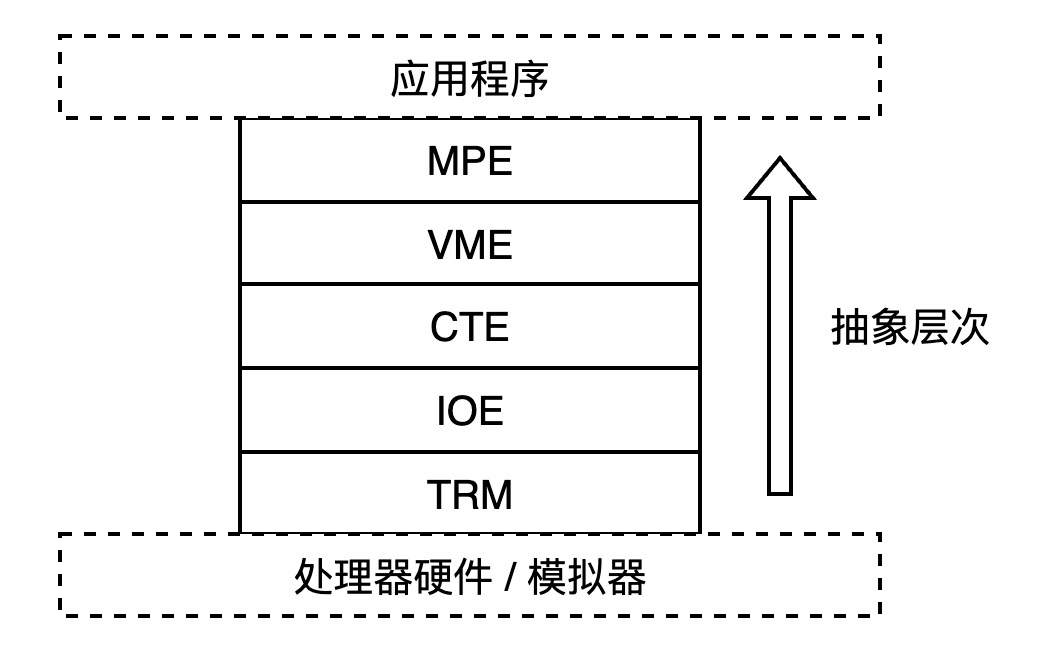
\includegraphics[width=1\linewidth]{assets/13/am-arch.jpg}
  \caption{AM的层次结构}
  \label{fig:am-arch}
\end{figure}

最底层为TRM层，即Turing Machine。
在该层次中，AM提供了一个最简单的、可供计算机进行计算的运行时环境，包括以下功能：

\begin{itemize}
\item
  使用数组\texttt{heap}维护了一块内存空间，即``堆区''，提供给上层程序使用；
\item
  提供了程序入口\texttt{main}，其中包括一个循环；
\item
  提供了程序终止运行的函数\texttt{halt}，上层程序调用该函数即可使其停机；
\item
  提供了打印字符的函数\texttt{putch}。
\end{itemize}

第二层为IOE层，即Input / Output Extension。
该层提供了更多的输入输出方法，例如按格式输出函数\texttt{printf}，以及串口等外设的驱动。
第三层为CTE（Context Extension）层，提供了中断异常的相关服务，完成了上下文的保存恢复工作，并向上层提供了自陷函数\texttt{yield}。
第四层和第五层分别为VME（Virtual Memory Extension）和MPE（Multi-Processor Extension），他们分别实现了虚拟存储和多处理器的相关工作。

在完成AM中全部层次或部分层次的开发后，学生可使用该环境提供的系统服务，编写一些应用程序。
借助南京大学开发的NEMU（NJU Emulator）体系结构模拟器，学生可将自己编写的程序，通过裸机运行时环境AM，运行在体系结构模拟器NEMU上。
其中，学生编写的程序会使用到AM向应用程序提供的系统服务。
在此过程中，学生将对程序运行在计算机上的过程有更深入的理解。

裸机运行时环境AM具有两个特点。
第一，AM将操作系统进行了足够的简化和模块化。
在每个层次中，使用者只需要实现本层次中最基础的功能，即可得到一个具有一定功能的计算机系统，符合敏捷开发流程中对原型开发的重视原则。

第二，AM对计算机系统提供了丰富的抽象层次，层次间互相解耦，因此具有很高的扩展性。
对于其他指令集架构的硬件，AM只需要重构TRM层即可在新的硬件上完成移植。
若要在AM中增加外设，例如增加声卡、网卡，只需要对IOE层进行扩展，提供新的服务函数即可。
因此，使用者可根据需要对AM进行快速增量迭代。

\subsection{在AM上实现极简操作系统}\label{sec:13-operating-system-024}

基于AM的高度层次化和模块化特点，使用者可以使用它开发出系统软件，也就包括操作系统。
在CPU设计结束后，自行设计一套操作系统并且在上面运行，可以打通计算机硬件到计算机软件的整个体系，加深对计算机系统的整体理解。
本节将介绍如何在AM上实现一个简单的操作系统。

为了适配LA32R指令集架构，首先需要将AM的TRM层进行重构。

% 代码语言：BookC
\begin{CodeBlock}[language=BookC]
#include <am.h>
#include <la32r.h>
#include <klib.h>
#include <la32r-csr.h>

extern char _heap_start;
extern char _pmem_end;
int main(const char *args);
void __am_init_uartlite(void);
void __am_uartlite_putchar(char ch);

_Area _heap = {
  .start = &_heap_start,
  .end = &_pmem_end,
};

void _putc(char ch) {
  __am_uartlite_putchar(ch);
}

void _halt(int code) {
  // set $a0 = code
  __asm__ volatile("add.w $r4, %0, $r0" : :"r"(code));
  // syscall 0x11 is nemu trap
  __asm__ volatile("syscall 0x11");

  // should not reach here during simulation
  printf("Exit with code = %d\n", code);

  // should not reach here on FPGA
  while (1);
}

inline void _cache_init()
{
  // invalid icache & dcache, just need two insts due to hardware implementation
  __asm__ __volatile__("cacop 0, $r0, 0" : : : "memory");
  __asm__ __volatile__("cacop 1, $r0, 0" : : : "memory");
}

// dmw0 map va : 0xa0000000 - 0xbfffffff -> pa : 0xa0000000 - 0xbfffffff (SUC PLV0 PLV3)
// dmw1 map va : 0x0 - 0x1fffffff -> pa : 0x0 - 0x1fffffff (CC PLV0 PLV3)
// note that pa : 1fe001e0 - 1fe001d0 has mmio to uart8250 device, so do not use va : 1fe00000 - 1fe0ffff as CC memory!
inline void _dmw_init()
{
  uint32_t dmw0 = 1 | (1 << DMW_PLV3_OFFSET) | (STRONGLY_ORDERED_UNCACHED << DMW_MAT_OFFSET) | (5 << DMW_PSEG_OFFSET) | (5 << DMW_VSEG_OFFSET);
  uint32_t dmw1 = 1 | (1 << DMW_PLV3_OFFSET) | (COHERENT_CACHED << DMW_MAT_OFFSET) | (0 << DMW_PSEG_OFFSET) | (0 << DMW_VSEG_OFFSET);
  csr_write(csr_dmw0, dmw0);
  csr_write(csr_dmw1, dmw1);

  csr_masked_write(csr_crmd, (0 << CRMD_DA_OFFSET) | (1 << CRMD_PG_OFFSET) | (1 << CRMD_DATF_OFFSET) | (1 << CRMD_DATM_OFFSET), CRMD_DA_MASK | CRMD_PG_MASK | CRMD_DATF_MASK | CRMD_DATM_MASK);
}

void _trm_init() {
  __am_init_uartlite();
  _cache_init();
  _dmw_init();
  extern const char __am_mainargs;
  int ret = main(&__am_mainargs);
  _halt(ret);
}
\end{CodeBlock}

在这段代码中，完成了对\texttt{\_heap}的定义，为上层提供了内存区域。在\texttt{\_putc}函数中，使用uart串口打印uart输出。如果希望有其他的输出方式，也可以用其他方法实现\texttt{\_putc}函数。本代码也重写了\texttt{\_halt}函数，作为停止运行的标志，方便进行仿真验证。该函数中进行了系统调用\texttt{syscall\ 0x11}，在仿真验证时，体系结构模拟器NEMU将识别该系统调用，并作为程序运行结束的标志。

由于LA32R架构中，Cache模块的初始化可不由硬件完成，因此在应用程序在待测处理器上运行之前，需要对Cache模块进行清空。上述代码的\texttt{\_cache\_init}函数就完成了该操作，使用LA32R架构规定的\texttt{cacop}指令进行了Cache初始化。

另外，LA32R架构提供了一种特殊的直接映射配置窗口机制。
在处理器处于映射地址模式时，处理器可通过CSR中设置的寄存器直接进行地址翻译，而不通过TLB。
在这段启动代码的编写工作中，也对CSR中的直接映射配置窗口寄存器（\texttt{DMWO},\texttt{DMW1}）进行了配置，从而保证上电后处理器可正常运行程序，即代码中的\texttt{\_dmw\_init}函数。

\texttt{\_trm\_init}是RTM层的顶层函数，将要调用其他函数，以进行环境的初始化工作。

为了方便进行系统的编写，需要对LA32R架构特有的CSR寄存器在代码中进行设置，定义一系列宏，使编程时可直接使用。主要工作是将每个CSR寄存器的每个域进行设置。

% 代码语言：BookC
\begin{CodeBlock}[language=BookC]
#ifndef __LA32RCSR_H__
#define __LA32RCSR_H__

// csr addr define
// copy from regdef.h
#define csr_crmd      0x0
#define csr_prmd      0x1
#define csr_euen      0x2
#define csr_ectl      0x4 // ecfg
#define csr_estat     0x5
#define csr_era       0x6
#define csr_badv      0x7
#define csr_eentry     0xc
#define csr_tlbidx    0x10
#define csr_tlbehi    0x11
#define csr_tlbelo0    0x12
#define csr_tlbelo1    0x13
#define csr_asid      0x18
#define csr_pgdl      0x19
#define csr_pgdh      0x1a
#define csr_pgd       0x1b
#define csr_cpuid    0x20
#define csr_save0     0x30
#define csr_save1     0x31
#define csr_save2     0x32
#define csr_save3     0x33
#define csr_tid       0x40
#define csr_tcfg      0x41
#define csr_tval      0x42
#define csr_ticlr     0x44
#define csr_llbctl    0x60
#define csr_tlbrentry 0x88
#define csr_dmw0      0x180
#define csr_dmw1      0x181

// csr mask define
#define CRMD_PLV_MASK       0x3
#define CRMD_IE_MASK        0x4
#define CRMD_DA_MASK        0x8
#define CRMD_PG_MASK        0x10
#define CRMD_DATF_MASK      0x60
#define CRMD_DATM_MASK      0x180

#define PRMD_PPLV_MASK      0x3
#define PRMD_PIE_MASK       0x4

#define ECFG_LIE_MASK       0x1bff

#define ESTAT_SWI_MASK      0x3
#define ESTAT_HWI_MASK      0x3fc
#define ESTAT_TI_MASK       0x800
#define ESTAT_IPI_MASK      0x1000
#define ESTAT_ECODE_MASK    0x3f0000
#define ESTAT_ESUBCODE_MASK 0x7fc00000

#define LLBCTL_ROLLB_MASK   0x1
#define LLBCTL_WCLLB_MASK   0x2
#define LLBCTL_KLO_MASK     0x4

#define TLBIDX_INDEX_MASK   0xffff
#define TLBIDX_PS_MASK      0x3f000000
#define TLBIDX_NE_MASK      0x80000000

#define TLBELO_V_MASK       0x1
#define TLBELO_D_MASK       0x2
#define TLBELO_PLV_MASK     0xc
#define TLBELO_MAT_MASK     0x30
#define TLBELO_G_MASK       0x40
#define TLBELO_PPN_MASK     0xfffff00

#define ASID_ASID_MASK      0x3ff

#define DMW_PLV0_MASK       0x1
#define DMW_PLV3_MASK       0x8
#define DMW_MAT_MASK        0x30
#define DMW_PSEG_MASK       0xe000000
#define DMW_VSEG_MASK       0xe0000000

#define TCFG_EN_MASK        0x1
#define TCFG_PERIODIC_MASK  0x2
#define TCFG_INITVAL_MASK   0xfffffffc

#define TICLR_CLR_MASK      0x1

// csr field right bits, Indicates how many bits are on the right side of this field
#define CRMD_IE_OFFSET       2
#define CRMD_DA_OFFSET       3
#define CRMD_PG_OFFSET       4
#define CRMD_DATF_OFFSET     5
#define CRMD_DATM_OFFSET     7

#define PRMD_PIE_OFFSET      2

#define ESTAT_ECODE_OFFSET   16
#define ESTAT_ESUBCODE_OFFSET    22

#define LLBCTL_WCLLB_OFFSET  1
#define LLBCTL_KLO_OFFSET    2

#define TLBIDX_PS_OFFSET     24
#define TLBIDX_NE_OFFSET     31

#define TLBEHI_VPPN_OFFSET   13

#define TLBELO_D_OFFSET      1
#define TLBELO_PLV_OFFSET    2
#define TLBELO_MAT_OFFSET    4
#define TLBELO_G_OFFSET      6
#define TLBELO_PPN_OFFSET    8

#define DMW_PLV3_OFFSET      3
#define DMW_MAT_OFFSET       4
#define DMW_PSEG_OFFSET      25
#define DMW_VSEG_OFFSET      29

#define TCFG_PERIODIC_OFFSET 1
#define TCFG_INITVAL_OFFSET  2

// ecode
#define INT_ECODE   0x0
#define PIL_ECODE   0x1
#define PIS_ECODE   0x2
#define PIF_ECODE   0x3
#define PME_ECODE   0x4
#define PPI_ECODE   0x7
#define ADEF_ECODE  0x8
#define ALE_ECODE   0x9
#define SYS_ECODE   0xb
#define BRK_ECODE   0xc
#define INE_ECODE   0xd
#define IPE_ECODE   0xe
#define FPD_ECODE   0xf
#define FPE_ECODE   0x12
#define TLBR_ECODE  0x3f

#define STRONGLY_ORDERED_UNCACHED 0
#define COHERENT_CACHED           1

// csr R/W copy and modify from nexus-am
#define __ASM_STR(x)    #x

// csrrd rd, csr_num
#define csr_read(csr)       \
    ({                      \
        register unsigned int __v;  \
        __asm__ __volatile__("csrrd %0 , " __ASM_STR(csr) \
                            : "=r"(__v)    \
                            :                  \
                            : "memory");       \
        __v;    \
    })

// csrwr rd, csr_num
#define csr_write(csr, val)                                        \
    ({                                                         \
        unsigned int __v = (unsigned int)(val);          \
        __asm__ __volatile__("csrwr %0, " __ASM_STR(csr)  \
                     : "+r"(__v)                           \
                     :                    \
                     : "memory");                  \
    })

// csrxchg rd, rj, csr_num
#define csr_masked_write(csr, val, wmask)                                        \
    ({                                                         \
        unsigned int __v = (unsigned int)(val);          \
        unsigned int __wmask = (unsigned int)(wmask);          \
        __asm__ __volatile__("csrxchg %0, %1, " __ASM_STR(csr)  \
                     : "+r"(__v)                          \
                     : "r"(__wmask)                   \
                     : "memory");                  \
    })

#define TLB_ENTRY_NUM 32

#define tlbsrch() __asm__ __volatile__("tlbsrch": : : "memory")

#define tlbrd() __asm__ __volatile__("tlbrd" : : : "memory")

#define tlbwr() __asm__ __volatile__("tlbwr" : : : "memory")

#define tlbfill() __asm__ __volatile("tlbfill" : : : "memory")

#define invtlb(op, asid, va)                                        \
    ({                                                         \
        unsigned int __asid = (unsigned int)(asid);          \
        unsigned int __va = (unsigned int)(va);          \
        __asm__ __volatile__("invtlb " __ASM_STR(op) ", %0, %1"  \
                     :                            \
                     : "r"(__asid), "r"(__va)                   \
                     : "memory");                  \
    })

#pragma pack(8)
typedef union {
  struct {
    uint32_t E    : 1;
    uint32_t ASID : 10;
    uint32_t G    : 1;
    uint32_t PS   : 6;
    uint32_t VPPN : 19;
    uint32_t      : 27;    
  };
  uint64_t val;
} EntryHi;
#pragma pack()

typedef union {
  struct {
    uint32_t V     : 1;
    uint32_t D     : 1;
    uint32_t MAT   : 2;
    uint32_t PLV   : 2;
    uint32_t PPN   : 24;
    uint32_t pad0  : 2;
  };
  uint32_t val;  
} EntryLo;
\end{CodeBlock}

为了实现操作系统，还需要编写上电后直接运行的程序。在这段程序中，需要对CPU进行进一步的初始化。

% 代码语言：BookLoongArch
\begin{CodeBlock}[language=BookLoongArch]
.section entry, "ax"
.globl _start
.type _start, @function

// start from pc = 0x1c000000
_start:

  // reset cache
  bl _cache_init
  
  // dmw0 map va : 0x0 - 0x1fffffff -> pa : 0x0 - 0x1fffffff (SUC PLV0 PLV3)  for device access
  // dmw1 map va : 0x80000000 - 0x9fffffff -> pa : 0x0 - 0x1fffffff (CC PLV0 PLV3) for memory access
  bl _dmw_init
  
  // set stack pointer to va 0x87000000 (set stack to a higher memory space for _relocate() tempory use)
  ori     $sp, $zero, 0
  lu12i.w $sp, 0x8700
  
  // do relocate, move code and data from spi flash to memory
  bl _relocate

  // jump to memory
  li.w    $t0, 0x80000100
  jirl    $zero, $t0, 0

  .org 0x100

  la.local $sp, _stack_pointer
  bl _trm_init

_excp:
  bl _excp_dispatch
\end{CodeBlock}

这段代码先调用了刚刚定义的\texttt{\_cache\_init}等函数，之后对地址映射窗口进行配置，设置了栈指针，并跳转到\texttt{\_relocate}进行清空工作。之后将跳转到\texttt{\_trm\_init}进行初始化，内部将跳转到程序的运行入口。

还需要编写链接脚本，以保证内存大小等参数正常配置，在链接时进行正确的装载。

% 代码语言：BookLinker
\begin{CodeBlock}[language=BookLinker]
pmem_base = 0x80000000;

OUTPUT_FORMAT(elf32-loongarch);

MEMORY {
  ram (rwxa) : ORIGIN = 0x80000000, LENGTH = 128M
}

INCLUDE "section.ld"
\end{CodeBlock}

% !TeX root = ../main.tex
% 原始章节：14-software.Rmd

\chapter{应用软件适配}\label{chap:14-software}

\section{Linux 系统 init 进程介绍}\label{sec:14-software-001}

在 Linux 系统中，\texttt{init} 进程是系统启动后第一个运行的进程，也是所有其他进程的父进程。它承担以下功能：

\begin{enumerate}
\item \textbf{启动系统服务}：\texttt{init} 负责在系统启动过程中加载和启动各种系统服务和守护进程（例如网络服务、日志服务等）。它通过读取特定的初始化脚本来确定哪些服务需要启动。
\item \textbf{设定运行级别}：\texttt{init} 根据配置文件（如 \texttt{/etc/inittab} 或 \texttt{systemd} 下的配置）决定系统启动后应该处于什么运行级别（runlevel），比如单用户模式、多用户模式或图形化模式等。传统的运行级别包括：
\begin{itemize}
\item \texttt{0}：关机
\item \texttt{1}：单用户模式
\item \texttt{2-5}：多用户模式（不同的服务集）
\item \texttt{6}：重启
\end{itemize}
\item \textbf{管理进程生命周期}：\texttt{init} 负责监控系统中的其他进程。当某个进程终止时，它会清理资源并进行相关的管理工作。特别是，孤立的子进程会被 \texttt{init} 接管。
\item \textbf{系统关闭和重启}：在系统关机或重启时，\texttt{init} 会依次停止所有运行中的服务，确保系统能安全地退出。
\end{enumerate}


现代 Linux 系统通常使用 \texttt{systemd} 替代传统的 SysV \texttt{init}，它提供了更强大的并行化启动和依赖管理功能。
但对于我们嵌入式处理器芯片的使用场景，使用 systemd 可能较为臃肿。我们一般选用 Busybox 作为 init，避免 systemd 的臃肿和复杂度。

使用 Busybox 之后，我们得到了一个最小化的可用 Linux 操作系统。但 Busybox 中的 Init 基本上不会为我们做任何的初始化工作，
因此使用 Busybox 的场景下，我们需要根据我们的需求，自行编写一些 Init 脚本放在合适位置，以供 busybox 在系统启动后自动调用，完成额外初始化工作。

如对网络，我们可编写脚本，在启动后使用 ip 命令配置本地网络地址，使能网络端口，配置默认路由及域名解析服务等。

\section{Busybox 工具集介绍}\label{sec:14-software-002}

对于我们设计的处理器，它们的存储和内存资源非常有限，完全不像我们日常使用的电脑那样有着充足的硬件资源。
在这种情况下，我们需要一套轻量级的工具来为系统提供基础的命令行功能。这时，BusyBox 就成了一个理想的选择。

BusyBox 可以看作是一个多合一的工具箱，它把 Linux 系统中许多常用的命令打包在一起。
比如我们平时在 Linux 终端中使用的 ls、cp、rm 这些命令，BusyBox 都能提供，虽然这些命令在功能上可能稍微简化了一些，但对于嵌入式设备来说，已经绰绰有余了。

可以这样理解它：在一个典型的 Linux 系统中，ls 是一个单独的可执行文件，cp 也是一个单独的可执行文件，每个工具都有自己的一份代码。
而在 BusyBox 中，这些命令共享同一个可执行文件，只是根据输入的命令参数来执行不同的功能。
这样做的好处非常明显------体积大大缩小，而且减少了系统的复杂性。

BusyBox 的另一个特别之处在于它的可定制性。
你可以根据设备的需求，在编译 BusyBox 时选择你真正需要的工具。
比如，如果你的嵌入式设备不需要处理压缩文件，你就可以在编译时禁用 gzip 和 tar，这进一步减小了可执行文件的体积。
实际上，在很多嵌入式 Linux 发行版中，比如 OpenWRT 或者 Buildroot， BusyBox 被广泛使用。
这些发行版本质上都是为了在资源受限的环境下运行，因此必须保证系统既能提供必要的功能，又不会占用太多的存储和内存。

\section{交叉编译 Busybox}\label{sec:14-software-003}

交叉编译 BusyBox 可能看起来有些复杂，但其实是非常简单的。而对于其它用户程序的编译流程，也是差不多相似的。你可以举一反三。

交叉编译的主要目的是在一个开发环境中为不同的目标平台（比如嵌入式设备）编译程序。具体到我们这里，就是在 x86\_64 的 Linux 平台交叉编译到 LoongArch 的平台。

\textbf{第一步：准备交叉编译工具链}

交叉编译的关键在于你需要一个``工具链''（Toolchain），它包含编译器、链接器、库等，专门为目标平台构建程序。
我们这里需要使用由龙芯官方提供的 LoongArch32R 的 8.3.0 GCC 工具链。
我们从官方下载安装相应的交叉编译工具链即可。

\textbf{第二步：下载 BusyBox 源代码}

从 BusyBox 官方 Git 镜像仓库获取最新的源码：

% 代码语言：bash
\begin{CodeBlock}
git clone git@github.com:mirror/busybox.git
cd busybox
\end{CodeBlock}

\textbf{第三步：配置编译选项}

现在，你需要配置 BusyBox 以便为目标设备编译。BusyBox 提供了一个交互式的配置工具，类似于内核配置工具 menuconfig，可以让你选择编译哪些命令。

首先，你可以使用 BusyBox 自带的默认配置作为基础：

\texttt{make\ defconfig}

这会生成一个默认的配置文件 .config，其中包含了 BusyBox 的基本命令集。

接下来，为了进行交叉编译，你需要告诉 BusyBox 使用哪一个编译器。这就是我们之前准备的交叉编译工具链：

\texttt{make\ menuconfig}

进入配置菜单后，选择以下路径：

进入 ``Settings'' → ``Build Options'' → ``Cross Compiler prefix''
将前缀设置为你交叉编译器的名称，比如：loongarch32r-linux-gnusf-
你也可以在这个菜单中进一步裁剪 BusyBox 的功能，根据设备的需求启用或禁用特定命令。

\textbf{第四步：编译 BusyBox}

配置完成后，就可以开始编译了。输入以下命令：

\begin{CodeBlock}
make -j$(nproc)
\end{CodeBlock}

这会调用交叉编译器，为目标设备生成 BusyBox 二进制文件。\texttt{-j\$(nproc)} 参数会使用你电脑的所有处理器核心来加速编译。

\textbf{第五步：安装 BusyBox}

编译完成后，你可以将 BusyBox 安装到一个指定的目录中。这通常是一个临时的根文件系统目录，稍后你可以将它打包并上传到设备上：

\begin{CodeBlock}
make install
\end{CodeBlock}

安装过程会生成一个基本的嵌入式 Linux 文件系统结构，所有的 BusyBox 命令都将软链接到一个单一的 BusyBox 可执行文件上。你可以在生成的目录中查看这些链接。

\textbf{第六步：部署到设备}

现在你已经有了编译好的 BusyBox 和它的相关文件。接下来就是将它复制到将作为我们启动 sd 卡的根目录：

\texttt{sudo\ cp\ -r\ \_install/*\ /some\_sdcard\_used\_as\_rootfs/}

注意，这里一定需要使用 root 用户进行复制。
部署完成后，在我们的处理器上运行 Linux，并指定根文件系统为我们刚才构建的 SD 卡 ext4 分区即可。

% !TeX root = ../main.tex
% 原始章节：15-chip-impl-preparation.Rmd

\chapter{芯片实现准备}\label{chap:15-chip-preparation}

\section{各类型IP替换}\label{sec:15-chip-preparation-001}

\subsection{从 FPGA 到芯片}\label{sec:15-chip-preparation-002}

在集成电路设计中，FPGA（现场可编程门阵列）验证环境与流片验证环境存在一定的差异。FPGA
通常用于原型验证和早期开发阶段，而流片后的芯片则是最终产品，两者的设计目标和实现方法有所不同。在从
FPGA 转向芯片的过程中，需要对一些关键的 IP
核进行替换或重新设计，以满足流片环境的需求。

\textbf{FPGA 验证环境与流片验证环境的主要区别}

\begin{enumerate}
\def\labelenumi{\arabic{enumi}.}
\tightlist
\item
  \textbf{硬件结构的不同}:

  \begin{itemize}
  \tightlist
  \item
    \textbf{FPGA}: FPGA
    具有可编程的逻辑单元、可重配置的布线架构和大量内置的 IP 核，如
    PLL、Block RAM 等。这些特性使 FPGA
    非常灵活，能够快速实现和验证复杂的数字电路设计。
  \item
    \textbf{流片芯片}:
    流片后的芯片是经过工艺制造的固定逻辑电路，其结构不可更改，必须在设计阶段完全确定。流片芯片通常对性能、功耗和面积进行优化，这些方面的优化需要针对特定的工艺技术进行。
  \end{itemize}
\item
  \textbf{设计流程的不同}:

  \begin{itemize}
  \tightlist
  \item
    \textbf{FPGA 设计}: FPGA
    设计主要关注功能验证和快速原型实现。设计者可以通过工具链生成位流文件，将设计下载到
    FPGA 上进行验证。这一过程相对快速且灵活，可以频繁迭代修改。
  \item
    \textbf{流片设计}:
    流片设计需要通过一系列复杂的步骤，包括逻辑综合、物理设计、版图生成、时序分析和功耗优化。由于流片成本高昂，设计在进入流片阶段之前必须经过严格的验证和测试。
  \end{itemize}
\end{enumerate}

由于FPGA与ASIC在结构、性能上各不相同，ASIC是基于标准单元库，FPGA用的是厂商提供的宏单元模块，因此首先要进行寄存器传输级(RTL)代码的修改。

\textbf{FPGA 到芯片中需要替换的 IP 核}

在从 FPGA 转向流片芯片的过程中，一些 IP
核需要进行替换或重新设计，以适应流片环境的需求。这些 IP
核包括但不限于以下几个重要组件：

\begin{enumerate}
\def\labelenumi{\arabic{enumi}.}
\item
  \textbf{PLL（Phase-Locked Loop）}:

  数字电路中，时钟是整个电路最重要、最特殊的信号。在ASIC中，用布局布线工具来放置时钟树，利用代工厂提供的PLL进行时钟设计。FPGA中通常已经配置一定数量的PLL宏单元，并有针对时钟优化的全局时钟网络，一般是经过FPGA的特定全局时钟管脚进入FPGA内部，后经过全局时钟BUF适配到全局时钟网络的，这样的时钟网络可以保证相同的时钟沿到达芯片内部每一个触发器的延迟时间差异是可以忽略不计的。因此时钟单元也是需要进行转换的。
\item
  \textbf{Block RAM}:

  存储单元是必须进行代码转换的，ASIC中的存储单元通常用代工厂所提供的Memory
  Compiler来定制，它可以生成.gsp、.v等文件。.v文件只用来做功能仿真，通常不能综合。而最后流片时，只需将标准提供给代工厂。如果直接将FPGA代码中的存储单元作为ASIC的输入，通常综合器是综合不出来的，即使能综合出来，也要花费很长时间，并且资源消耗多、性能不好。因此存储单元要进行代码转换。
\item
  \textbf{Memory Controller}:

  FPGA 中的 Memory Controller 通常使用 IP 核实现，支持多种内存类型，如
  DDR、SRAM 等。在流片设计中，Memory Controller
  需要针对特定的内存类型进行设计，特别是在高速存储器接口设计中，必须确保满足严格的时序和电气性能要求。
\item
  \textbf{其他专用 IP 核}:

  除了上述常见的 IP 核外，其他一些 IP
  核也可能需要替换或定制化设计。例如，寄存器堆、乘法器或其他无法获得代码的FPGA
  IP核。
\end{enumerate}

\subsection{PLL替换}\label{sec:15-chip-preparation-003}

本文以SMIC180工艺库为例介绍相关操作，\textbf{出于学习目的}，该工艺库可从一些网络途径获取。

在FPGA平台，我们一般使用\href{https://www.xilinx.com/products/intellectual-property/clocking_wizard.html}{Clocking
Wizard}
IP来生成不同频率的时钟信号，但在芯片流片时需要使用制造商工艺库中提供的PLL
IP来实现这一功能，本文基于\texttt{S018PLLGS\_LC}介绍如何使用PLL

\textbf{IP引脚定义}

\begin{longtable}[]{@{}
  >{\raggedright\arraybackslash}p{(\linewidth - 4\tabcolsep) * \real{0.1944}}
  >{\raggedright\arraybackslash}p{(\linewidth - 4\tabcolsep) * \real{0.1944}}
  >{\raggedright\arraybackslash}p{(\linewidth - 4\tabcolsep) * \real{0.6111}}@{}}
\toprule\noalign{}
\begin{minipage}[b]{\linewidth}\raggedright
引脚名称
\end{minipage} & \begin{minipage}[b]{\linewidth}\raggedright
输入/输出
\end{minipage} & \begin{minipage}[b]{\linewidth}\raggedright
描述
\end{minipage} \\
\midrule\noalign{}
\endhead
\bottomrule\noalign{}
\endlastfoot
AVDD & 电源 & 专用模拟电源供电 +1.8V \\
AVSS & 地 & 专用模拟地 \\
XIN & 输入 & 来自晶体振荡器或其他时钟源的参考时钟输入 \\
CLK\_OUT & 输出 & 可调输出时钟 \\
TST\_OUT & 输出 & 来自N或M分频器的测试模式输出 \\
N{[}4:0{]} & 输入 & 输入5位分频控制引脚，N{[}0{]}是最低位 \\
M{[}8:0{]} & 输入 & 反馈9位分频控制引脚，M{[}0{]}是最低位 \\
PLL\_TST{[}1:0{]} & 输入 & M和N分频器测试模式\newline{}PLL\_TST{[}1:0{]}=0:0 N分频器测试和正常操作\newline{}PLL\_TST{[}1:0{]}=1:1 M分频器测试\newline{}请在正常模式下将PLL\_TST{[}1:0{]}固定为0 \\
PD & 输入 & 断电控制；高电平有效 \\
OD{[}3:0{]} & 输入 & 输出分频控制引脚 \\
BP & 输入 & 绕过PLL；高电平有效 \\
OE & 输入 & CLK\_OUT使能引脚，高电平有效 \\
\end{longtable}

\textbf{控制信号真值表}

\begin{longtable}[]{@{}lllllll@{}}
\toprule\noalign{}
PD & BP & OE & PLL\_TST\textless0\textgreater{} & PLL\_TST\textless1\textgreater{} & TST\_OUT & CLK\_OUT \\
\midrule\noalign{}
\endhead
\bottomrule\noalign{}
\endlastfoot
0 & 0 & 0 & 0 & 0 & XIN/N & CLK\_OUT \\
0 & 0 & 0 & 1 & 1 & XIN/M & XIN \\
X & 1 & 0 & X & X & 未定义 & XIN \\
X & X & 1 & X & X & 未定义 & 0 \\
其他 & & & & & 未定义 & 未定义 \\
\end{longtable}

\textbf{XIN与CLK\_OUT关系} \[
CLK\_OUT = X_\text{IN} \times \frac{M}{N} \times \frac{1}{NO} \times \frac{1}{2}
\]

\[
M = M_8 \times 256 + M_7 \times 128 + M_6 \times 64 + M_5 \times 32 + M_4 \times 16 + M_3 \times 8 + M_2 \times 4 + M_1 \times 2 + M_0 \times 1 + 2
\]

\[
N = N_4 \times 16 + N_3 \times 8 + N_2 \times 4 + N_1 \times 2 + N_0 \times 1 + 2
\]

\[
N_O = OD3 \times 8 + OD2 \times 4 + OD1 \times 2 + OD0 \times 1
\]

例如：当输入时钟为25MHz，而SoC需要一个133MHz的时钟时，可以按照如下方法定义

% 代码语言：BookSystemVerilog
\begin{CodeBlock}[language=BookSystemVerilog]
S018PLLGS_LC SOC_PLL(
  .XIN(clk_25m),
  .CLK_OUT(soc_clk),
  .N(5'b0_0001),
  .M(9'b0_0001_1110),
  .PLL_TST(2'b00),
  .RESET(1'b0),
  .PD(1'b0),
  .OD(4'b0001),
  .BP(1'b0),
  .OE(1'b0)
);
\end{CodeBlock}

此时\(M = 32, N = 3, NO = 1,CLK_{-}OUT=25 \times \frac{32}{3} \times \frac{1}{1} \times \frac{1}{2} = 133.\dot 3(MHz)\)

\subsection{SRAM替换}\label{sec:15-chip-preparation-004}

在FPGA中，我们一般使用Block Ram
IP或XPM宏来实现SRAM，在流片过程中则需要将这些SRAM替换为目标工艺库中的IP，我们需要使用制造公司提供的SRAM生成器来生成我们所需的SRAM。本文以
SMIC 0.18um Dual-Port Memory Compiler为例。

官方提供的安装包包括如下文件：

\begin{longtable}[]{@{}
  >{\raggedright\arraybackslash}p{(\linewidth - 2\tabcolsep) * \real{0.2055}}
  >{\raggedright\arraybackslash}p{(\linewidth - 2\tabcolsep) * \real{0.7945}}@{}}
\toprule\noalign{}
\begin{minipage}[b]{\linewidth}\raggedright
名称
\end{minipage} & \begin{minipage}[b]{\linewidth}\raggedright
作用
\end{minipage} \\
\midrule\noalign{}
\endhead
\bottomrule\noalign{}
\endlastfoot
S018DP.jar & 存储器生成器应用程序 \\
S018DP.csh & C Shell 设置文件 \\
S018DP\_ug.pdf & 用户手册 \\
S018DP.notes & 发布说明 \\
Library & GDS Smart Option 库，用于处理 GDS 文件并执行各种智能操作 \\
\end{longtable}

S018DP.csh文件内容如下

% 代码语言：BookShell
\begin{CodeBlock}[language=BookShell]
setenv MC_INSTALL_PATH `pwd`
java -jar S018DP.jar&
\end{CodeBlock}

运行该脚本可启动生成器的GUI界面

界面如图\ref{fig:sram-gen}所示：

\begin{figure}[htbp]
  \centering
  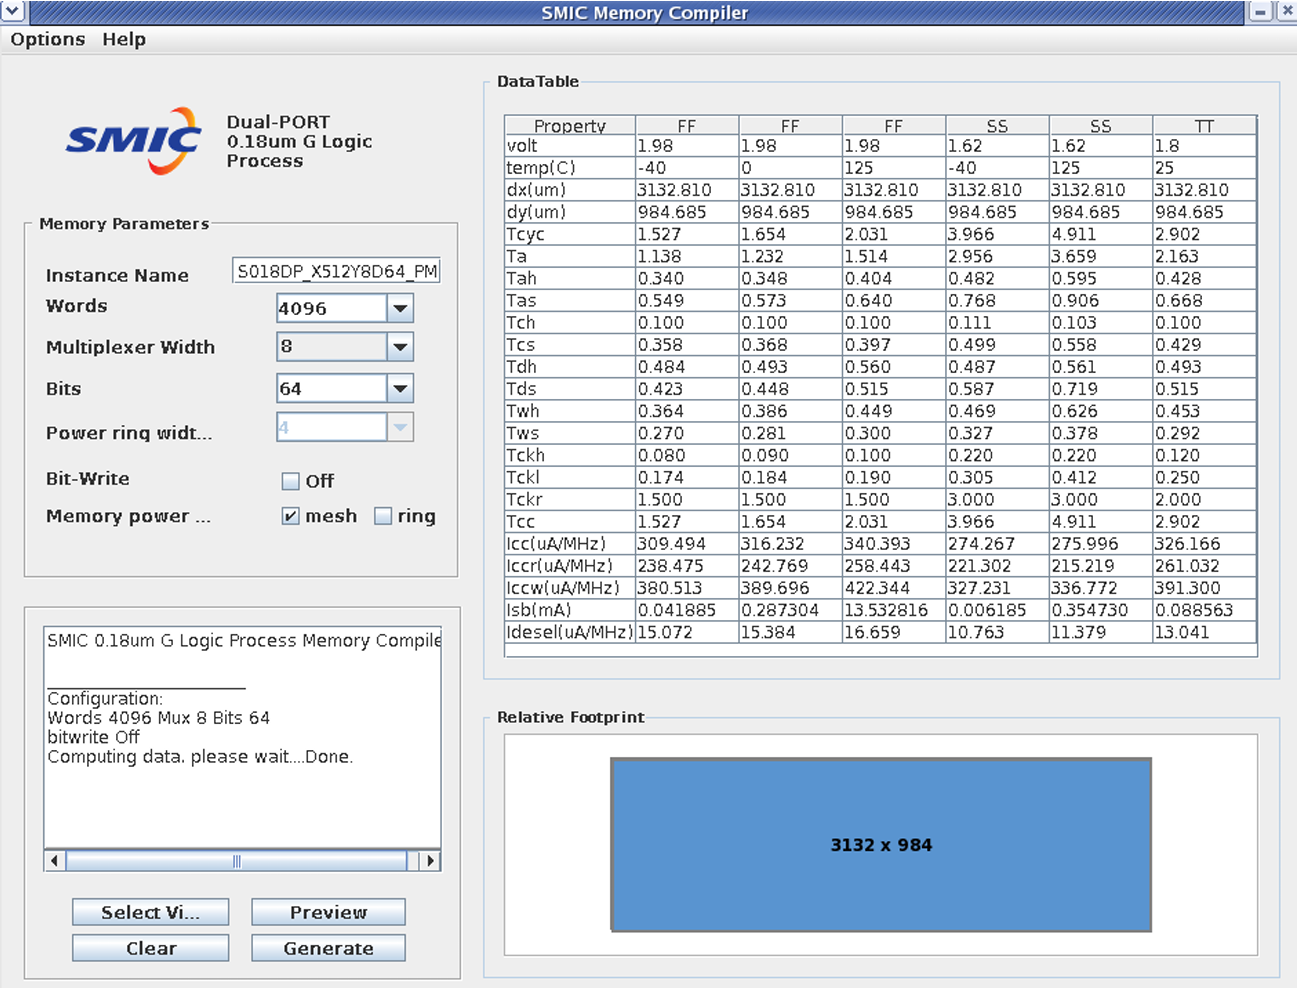
\includegraphics[width=1\linewidth]{assets/15/sram-gen.png}
  \caption{SRAM生成器GUI}
  \label{fig:sram-gen}
\end{figure}

\begin{enumerate}
\def\labelenumi{\arabic{enumi}.}
\item
  Memory Parameters（存储器参数）

  存储参数（Memory
  Parameters）面板包含输入字段和复选框。您可以通过从每个参数对应的下拉子菜单中选择所需的值或在输入字段中输入值来更改``字（Word）''、``多路复用器（Multiplexer）''和``位（Bits）''的值。此外，您还可以在复选框中选择``位写入（Bit-Write）''的开关状态（on/off）以及电源结构的``网格（mesh）''或``环形（ring）''选项。如果选择``环形''，则``电源环宽度''的下拉子菜单将变为可选状态，并且需要适当地设置电源环的尺寸，考虑到芯片级电源分配方法、电源环的数量、宽度和供电线连接的位置以及电流消耗。

  当您完成参数值的填写后，可以点击``预览（Preview）''按钮查看更新后的数据表面板（DataTable）、消息（Message）面板和相对占位面积（Relative
  Footprint）面板。例如，您可以为具有8192个字、64位和16多路复用器宽度的特定实例生成视图。在``字''下拉子菜单中选择8192，在``多路复用器宽度''下拉子菜单中选择16，在``位''下拉子菜单中选择64。然后点击``预览''按钮，数据表面板、消息面板和相对占位面积面板将会更新。
\item
  Relative Footprint （相对占位面积）

  相对占位面积面板显示了相应特定实例的纵横比。当您更改记忆参数并点击``预览''按钮后，相对占位面积将会更新。
\item
  Data Table （数据表）

  数据表显示了相应特定实例的拐角、布局尺寸、时序、电流和功耗信息。当您更改记忆参数并点击``预览''按钮后，数据表将会更新。
\item
  Message（信息）
  消息面板在您生成实例时显示相关消息。消息包括正在生成的实例的配置信息、正在生成的视图类型信息以及成功生成的提示信息。当您输入的值超出预定范围时，消息面板还会报告问题。
\end{enumerate}

当然也可以使用脚本生成：

% 代码语言：BookShell
\begin{CodeBlock}[language=BookShell]
#!/bin/bash
rm -rf *~
rm -rf *_RAM_DP_*
HEAD=S018DP

# words, bits, mux
config=(
'128 128 4'
'128 128 1'
'1024 16 4'
'1024 32 4'
'256 128 1'
'256 16 2'
'512 64 2'
'128 128 1'
)

for i in "${config[@]}"; do
  row=($i)
  W=${row[0]}
  B=${row[1]}
  M=${row[2]}
  RAM_NAME=${HEAD}_RAM_DP_W${W}_B${B}_M${M}
  echo $RAM_NAME
  rm -rf $RAM_NAME
  mkdir $RAM_NAME
  java -jar S018DP.jar -words $W -mux $M -bits $B -v -lib -pdf -gds -cdl -mbist -lef -powermesh -savepath ./$RAM_NAME -instname $RAM_NAME
\end{CodeBlock}

\subsection{SDRAM 控制器介绍}\label{sec:15-chip-preparation-005}

SDRAM控制器是一种用于控制同步动态随机存储器(SDRAM)的硬件设备。它能够实现高速、可靠的内存读写操作，并经常用于计算机、通讯系统和其他嵌入式应用中。SDRAM控制器有着复杂的内部工作机制，通过其内部的逻辑电路，实现对SDRAM存储器芯片的精细控制。

一个SDRAM控制器通常包含读写控制器、地址发生器、时钟控制器和数据缓冲等组件。它能够识别读取和写入命令，并控制存储器的读取和写入操作的执行时间。在操作过程中，SDRAM控制器先将外部指令和数据传输到数据缓冲区，然后再基于内部时钟更新SDRAM存储器中的数据。此外，SDRAM控制器还通过检测数据总线的情况，实现对数据的检查和纠错，以提高内存数据的可靠性。

SDRAM控制器的内部时钟频率非常高，通常达到百兆赫兹甚至更高。它能够对存储器按照指定的工作模式进行读写操作，如CAS时序、预充电和自刷新等。此外，SDRAM控制器还可以支持多通道、多控制器和多级缓存等高级特性，以大幅提高系统读写效率。

LainChip项目选定的内存控制器是SpinalHDL项目中的\href{https://github.com/SpinalHDL/SpinalHDL/tree/dev/lib/src/main/scala/spinal/lib/memory/sdram}{Sdram}库。SpinalHDL是一个高级的硬件描述语言，其以Scala语言为基础，提供一套框架，通过使用现代编程范式，打破了常用
HDL
中许多降低开发效率的限制。SpinalHDL项目中的Sdram控制器提供了AXI总线到SDRAM接口的翻译功能。该控制器分为前端与后端两部分，前端部分将AXI请求翻译为SDRAM的目标状态，后端根据前端传送的目标状态向SDRAM芯片发送对应的指令。该控制器支持AXI总线的突发传输特性，因此能进行较高速率的数据传输。

\section{EDA工具环境搭建}\label{sec:15-chip-preparation-006}

本节主要针对芯片实现过程中使用的EDA工具进行介绍，主要介绍所使用的工具类别及功能、流程等，并对照一些实际的脚本来参考如何使用EDA工具。

\subsection{EDA工具概览}\label{sec:15-chip-preparation-007}

芯片实现流程如下图\ref{fig:chip-flow}所示，其中每一步都会有对应的EDA工具来进行相应的操作，总体可分为前端设计与仿真、前端综合与评估、后端实现及验证三个部分。下面根据流程中常用的EDA工具按顺序进行一个简单的介绍（其中FPGA验证在第十二章已经描述，这里不再进行阐述）。

\begin{figure}[htbp]
  \centering
  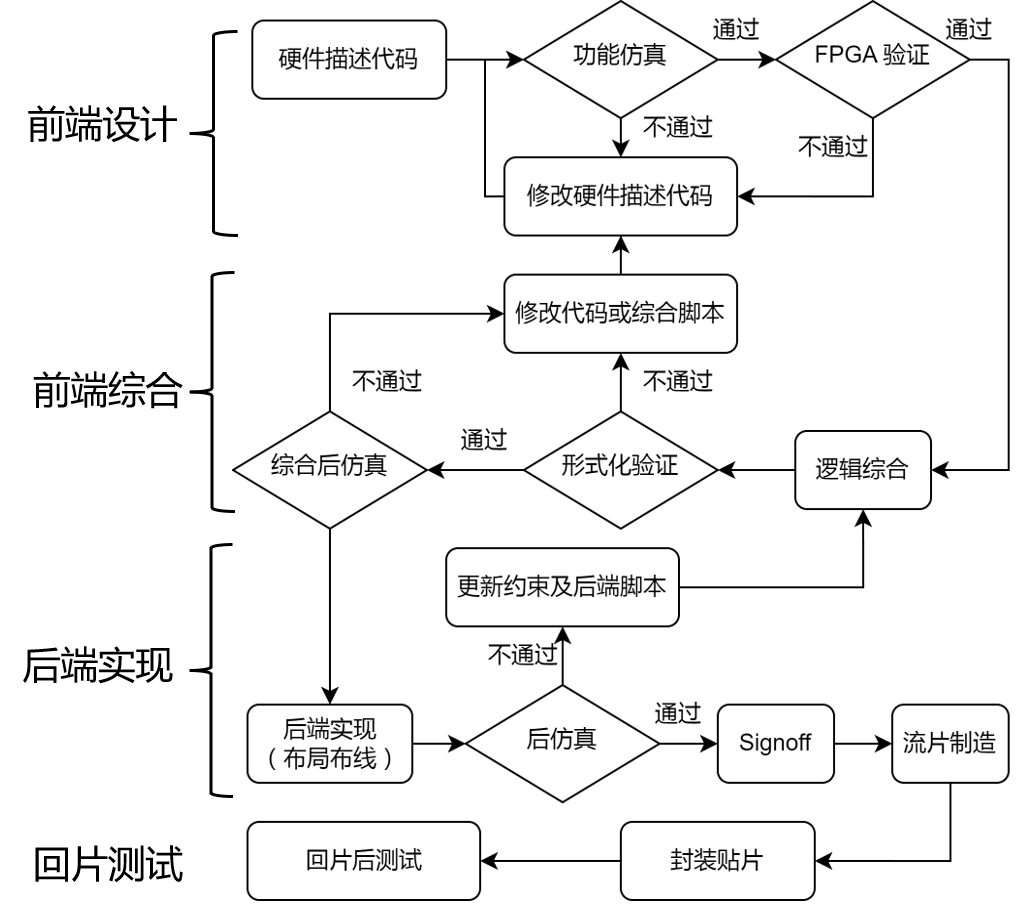
\includegraphics[width=0.5\linewidth]{assets/15/芯片设计流程.png}
  \caption{芯片设计流程示意图}
  \label{fig:chip-flow}
\end{figure}

\begin{enumerate}
\def\labelenumi{\arabic{enumi}.}
\tightlist
\item
  \textbf{芯片前端设计与仿真工具}：
\end{enumerate}

\begin{itemize}
\tightlist
\item
  \emph{Matlab}：在复杂的大型芯片项目中，往往前端设计还会涉及系统架构设计，通过matlab等首先对架构进行建模与评估，对整体设计划分模块。
\item
  \emph{VSCode}：在设计好架构之后就会通过硬件描述语言编写RTL代码（在本教材中除了VerilogHDL还有更抽象的Chisel等硬件描述语言来编写RTL），编写工具使用编辑器即可。
\item
  \emph{ModelSim}：是Mentor Graphics公司（先为Siemems
  EDA一部分）开发的一种高性能、交互式和可扩展的HDL仿真工具。
\item
  \emph{VCS}：全称为Verilog Compiled
  Simulator，是Synopsys公司推出的一款高性能、高容量的硬件描述语言（HDL）仿真工具。它主要用于验证数字集成电路（IC）设计，包括在寄存器传输级（RTL）和门级上的验证。
\item
  \emph{Iverilog}：全称为Icarus
  Verilog，是一个轻量级跨平台开源Verilog仿真软件，一般配合开源波形查看工具GTKWave配合使用。
\end{itemize}

\begin{enumerate}
\def\labelenumi{\arabic{enumi}.}
\setcounter{enumi}{1}
\tightlist
\item
  \textbf{芯片前端综合与评估工具}：
\end{enumerate}

\begin{itemize}
\tightlist
\item
  \emph{DC}：全称为Design
  Compiler，是Synopsys公司推出的用于芯片逻辑综合的工具。具体为将高抽象层级描述（寄存器传输级，RTL）转化为低层次的门级网表的工具，以实现电路逻辑功能的综合与优化等，并可以得到一个评估的时序、功耗、面积等。
\item
  \emph{PT}：全称为PrimeTime，是Synopsys公司推出的用于芯片静态时序分析的工具。具体功能为确保电路在时钟信号作用下能正确采样和保持数据，以及相较于DC工具更为全面的时序检查。一般在前端综合过后会使用PT工具进行更进一步的静态时序分析。在后续做完后端详细布线、提取参数后将生成的SPEF文件发送给PrimeTime获取更准确的STA分析结果。
\item
  \emph{PTPX}：全称为PrimeTime PX，是Synopsys公司推出的用于功耗分析的工具。
\item
  \emph{Formality}：Synopsys推出的用于形式验证的工具。主要功能为对综合后的网表与HDL设计进行对比，验证功能上的等价性，以保证逻辑综合过程没有改变HDL所描述的电路功能。
\end{itemize}

\begin{enumerate}
\def\labelenumi{\arabic{enumi}.}
\setcounter{enumi}{2}
\tightlist
\item
  \textbf{芯片后端实现与验证工具}：
\end{enumerate}

\begin{itemize}
\tightlist
\item
  \emph{Innovus}：Cadence公司推出的芯片后端实现的布局布线工具，即将逻辑综合后生成的门级电路通过物理方式连接起来，形成具有制造意义的版图的过程。
\item
  \emph{StarRC}：Synopsys推出的用于寄生参数提取的工具。
\item
  \emph{Voltus}：是一款Cadence公司推出的用于电源完整性分析和优化的EDA工具。
\item
  \emph{Calibre}：是Mentor公司推出的用于物理验证的EDA工具，对芯片版图进行检查，以确保其符合制造工艺和性能要求。具体包括设计规则检查（DRC）、版图与原理图一致性检查（LVS）、电气规则检查（ERC）等。
\end{itemize}

下面将针对这三种类别的EDA工具进行展开描述。

\subsection{芯片前端设计及仿真工具}\label{sec:15-chip-preparation-008}

首先编写HDL代码需要一个易用的代码编辑器，推荐使用\emph{VSCode}，因为其有较多的插件可以在代码设计的前期就检查到语法等方面的错误，也便于编辑代码。
在编写完成后需要对代码进行功能测试，测试工具包括\emph{VCS}、\emph{ModelSim}等，这里主要针对\emph{VCS}进行介绍与流程描述。

\emph{VCS}可支持多种抽象级别的仿真，包括行为级、RTL级、门级、SignOff等，这使得其可以支持芯片流程中的多个位置的仿真（前端RTL仿真到后端版图后仿真等）。\emph{VCS}工作原理分为两个阶段：编译和仿真。编译阶段，工具将Verilog/SystemVerilog源代码转换为中间表示形式，并生成可执行文件（通常为simv）。仿真阶段，通过执行这个可执行文件，对设计进行仿真，模拟这个运行过程并输出仿真结果。

具体的流程为：

\begin{itemize}
\item
  准备阶段：准备好Verilog源代码、testbench测试文件以及其他测试数据等相关文件。并创建一个file.list文件用于列出所有需要编译的Verilog文件路径，以方便后续使用VCS命令编译。
\item
  编译阶段：使用VCS命令编译，命令格式如下：
\end{itemize}

% 代码语言：BookShell
\begin{CodeBlock}[language=BookShell]
vcs -full64 -sverilog -debug_access+all -f file.list -timescale=1ns/1ns -l com.log
\end{CodeBlock}

其中，-full64表示在64位模式下编译，-sverilog表示支持SystemVerilog语言，-debug\_access+all用于保存调试过程中生成的各种文件，-f
file.list指定file.list文件作为输入，-timescale=1ns/1ns定义仿真时间单位，-l
com.log用于保存编译日志。

编译完成后，会生成一个名为simv的可执行文件（使用-o选项可以指定其他名字）。

\begin{itemize}
\tightlist
\item
  仿真阶段：在命令行中，通过执行simv文件来启动仿真，执行命令的基本格式如下：
\end{itemize}

% 代码语言：BookShell
\begin{CodeBlock}[language=BookShell]
./simv -l run.log
\end{CodeBlock}

仿真完成后，可以通过testbench中的\$display语句或其他输出方式查看仿真结果。此外，还可以使用VCS提供的图形化界面（如DVE）来观察波形和仿真结果。

\begin{itemize}
\tightlist
\item
  波形查看：在testbench中，可以通过添加下述语句调用dump
  fsdb函数来生成FSDB波形文件。例如：
\end{itemize}

% 代码语言：BookVerilog
\begin{CodeBlock}[language=BookVerilog]
initial begin  
  if ($test$plusargs("dumpfsdb")) begin  
    $fsdbDumpfile("TEST.fsdb");  
    $fsdbDumpvars(0, top_tb);  
  end  
end
\end{CodeBlock}

上述代码具体含义为：当检查仿真启动命令参数包含字符dumpfsdb时，将top\_tb模块及其所有子模块的信号进行转储为TEST.fsdb文件。之后使用Veridi查看波形，编译配置Veridi后打开上述.fsdb波形文件即可查看。

对于使用\emph{VCS}进行门级仿真，只需要将逻辑综合生成的网表文件（生成verilog）替换原来的RTL代码文件（若启用SDF反标，则执行类似下述命令）：

% 代码语言：BookShell
\begin{CodeBlock}[language=BookShell]
vcs -full64 -sverilog -sdf -max/typ/min:inst_name:sdf_path -debug_access+all -f 
file.list -timescale=1ns/1ns -l com.log
\end{CodeBlock}

其中max/typ/min选择一个，是指启用SDF文件中指定的最小值、典型值、最大值的一种，在实例inst\_name上进行反标时序。

\subsection{芯片前端综合与评估工具}\label{sec:15-chip-preparation-009}

在代码功能验证过后，将代码进行逻辑综合以将RTL设计转换成门级网表。\emph{DC}是Synopsys综合工具，内嵌了多种工具用于将RTL转化为网表并根据时序、面积等约束进行收敛。这里首先介绍\emph{DC}的使用流程，再用一个简单的脚本来说明\emph{DC}的具体使用过程。

\emph{DC}的使用流程：

\begin{itemize}
\tightlist
\item
  启动与环境初始化：可使用命令行启动与图形界面启动两种方式，启动过程需要读取初始化文件，用于初始化工具环境、库环境、工作路径等。
\item
  指定库文件：使用set target\_library来指定目标库、使用set
  link\_library来指定链接库等。工艺库由代工厂提供，如中兴国际SMIC180nm库等。
\item
  读入设计文件：使用read命令或analyze\&elaborate组合命令读入设计文件（如Verilog或systemVerilog文件，此时DC将设计文件转换成中间格式（如GTECH格式），便于后续处理。
\item
  施加设计约束：定义设计约束，包括面积约束、时序约束、DRC（设计规则检查）约束等；时序约束如定义时钟（create\_clock）、设置输入输出延迟（input\_delay、output\_delay）等；DRC约束如最大转换时间、最大扇出负载、最大负载电容等。
\item
  定义设计环境：设置工艺参数（如温度、电压等）和I/O端口属性（如负载、驱动、扇出等）；这些参数将影响设计综合及优化结果。
\item
  选择编译策略：DC进行优化的目的是权衡时序与面积，以满足用户对功能、速度、面积等要求。编译策略可选择compile与compile\_ultra（需要单独的license）两种。可添加high-effort指令来使DC更加努力达到所约束的目标。
\item
  输出文件：包括输出网表文件、报告文件等。报告包括时序报告、面积报告以及功耗报告等。用户可以根据输出报告来分析电路中可能存在的问题。
\end{itemize}

下面给出一个简化的\emph{DC}使用流程示例命令与脚本（假设已经由一个RTL设计文件design.v以及基本库文件stdcells.db、io\_cells.db等）：

bash文件：

% 代码语言：BookShell
\begin{CodeBlock}[language=BookShell]
#!/bin/bash  
  
# 设置环境变量，这里需要根据实际情况替换路径  
export SYNOPSYS_SIM_SETUP=/path/to/synopsys/setup_files  
# 注意：这通常是csh或tcsh脚本，如果是bash环境可能需要调整 
source $SYNOPSYS_SIM_SETUP/synopsys_dc_setup.csh   
  
# 切换到工作目录  
cd /path/to/your/working/directory  
  
# 清理之前的运行结果（可选）  
rm -rf csrc work report* *.db *.log *.vpd *.v *.sdf  
  
# 启动DC（这里以命令行模式为例，也可以启动design_vision图形界面）  
dc_shell -f run_dc.tcl  
\end{CodeBlock}

run\_dc.tcl文件，假设上述bash脚本与该文件在同一目录下：

% 代码语言：BookTcl
\begin{CodeBlock}[language=BookTcl]
# 设定工作库  
set_app_var search_path "+/path/to/std_cells_lib +/path/to/io_cells_lib"  
  
# 读取设计文件  
read_verilog -library WORK design.v  
  
# 定义库和链接库  
link  
  
# 设置目标库  
set target_library "typical.db"  
  
# 设置综合策略  
set_synthesis_strategy -effort high  
  
# 设置时钟  
create_clock -name clk -period 10 [get_ports clk]  
  
# 设置输入输出延迟（示例）  
set_input_delay -clock clk 3 [all_inputs]  
set_output_delay -clock clk 3 [all_outputs]  
  
# 编译设计
compile -map_effort high  
  
# 检查时序  
check_timing  
  
# 如果需要，可以导出网表和其他文件  
write_file -format verilog -hierarchy flat -output design_synth.v  
write_sdf -version 2.1 design.sdf  
  
# 结束DC会话（可选，通常在脚本末尾自动完成）  
exit
\end{CodeBlock}

一些实现过程根据需要配置，该脚本只是给出一个简单的示例。其他工具例如Formality等使用较为简单，这里不再详细阐述。

\subsection{芯片后端实现与验证工具}\label{sec:15-chip-preparation-010}

后端实现包括布局布线（也称为物理实现physical
design）、时序signoff、功耗与IR
signoff、物理验证等过程。这里主要针对芯片物理实现使用的EDA工具\emph{Cadence
Innovus}进行描述。

\emph{Cadence
Innovus}是一款高性能的电子设计自动化（EDA）工具，专为集成电路（IC）的物理设计和实现而开发。它主要用于大规模集成电路（VLSI）的布局布线，能够处理从RTL到GDSII的整个设计流程。Innovus具有强大的并行处理能力，支持现代节点的复杂工艺，并且能够优化功耗、性能和面积（PPA）。

具体的设计流程为：

\begin{itemize}
\tightlist
\item
  导入设计：包括综合生成的网表文件、库文件、IO约束文件等。
\item
  Floorplanning：定义芯片的总体结构和宏模块布局，确定芯片各部分的相对位置。
\item
  Placement：自动将标准单元放置到芯片平面上，同时考虑到信号延迟、功耗和面积等因素，自动调整单元位置执行放置优化。
\item
  时钟树综合（CTS）：设置并插入时钟树，确保所有时钟域内部的时钟信号能够同步达到。
\item
  布线（Routing）：执行全芯片的信号布线，并优化布线以减少信号延迟和交叉干扰（crosstalk）。
\item
  功耗分析与优化：分析芯片的动态与静态功耗，通过调整电压、频率或布局来优化功耗。
\item
  设计优化：针对性能、功耗和面积进一步优化，应用工程变更订单（ECO）进行最后的修正。
\end{itemize}

\section{仿真模拟与性能评估环境搭建}\label{sec:15-chip-preparation-011}

在集成电路（IC）设计过程中，仿真模拟和性能评估是验证设计符合预期要求的关键步骤。环境搭建需要精心规划，以确保仿真结果的准确性和可靠性。

\subsection{前仿与后仿}\label{sec:15-chip-preparation-012}

前仿（Pre-simulation）：指在实际物理实现之前对设计进行的仿真。通常在逻辑设计阶段（如RTL设计）进行。目的是验证设计在逻辑层面是否正确，检查功能是否符合预期。使用硬件描述语言（如Verilog或VHDL）编写的设计，在EDA工具（如ModelSim,
VCS等）中运行。可以使用波形查看器进行深入分析。

后仿（Post-simulation）：在设计的物理实现（如布局布线后）进行的仿真。使用的是更接近实际制造条件的数据。目的是验证物理实现是否影响了设计的功能，确认时序和性能指标。利用抽取出的布线信息和寄生参数（通过工具如StarRC），在EDA仿真工具中进行更接近真实条件的仿真。

\subsection{测试验证环境搭建}\label{sec:15-chip-preparation-013}

合适的测试平台和工具是设计验证的关键，仿真工具可以使用 Verilator 或 VCS。Verilator 是一种开源的硬件仿真器，主要用于将 Verilog 代码编译成 C++ 或 SystemC 代码，从而实现高效的仿真。它的设计目标是进行更快的仿真速度，而非完全的功能仿真; VCS 是 Synopsys 公司开发的一款商业级仿真器，广泛应用于芯片设计的各个阶段。它支持完整的 Verilog 和 SystemVerilog 语言，包括设计和验证的所有特性。VCS 能够进行精确的时序仿真、功耗分析、代码覆盖率报告等，适用于从功能验证到最终时序验证的各个阶段。波形查看工具可以采用 GTKWave，GTKWave 是一个开源的波形查看工具，主要用于查看数字电路仿真生成的波形数据。它支持多种仿真工具的输出格式，广泛用于硬件设计和验证过程中，帮助设计者分析仿真结果。

在完成处理器初步设计后，可以根据 \url{https://github.com/BUAA-CI-LAB/eula-env} 中的 README 接入 Eula-Env 集成芯片敏捷开发平台，其中可通过 Difftest 框架分析处理器执行周期、指令条数、IPC 等指标。

测试用例：开发一系列详尽的测试用例来覆盖所有可能的设计场景。这些测试用例应该旨在揭露功能缺陷和性能瓶颈。Eula-Env 中 AM 内置部分常用测试，例如功能测试、Coremark、Dhrystone 测试，同时包括 Linux 系统仿真，可以对处理器进行较为完善的测试。若需额外编写测试，可参考 \url{https://github.com/BUAA-CI-LAB/am/blob/master/README.md} 中关于创建单源/多源文件程序的介绍。

自动化测试：为了提高效率和准确性，应尽可能自动化测试过程。可使用 Python、Tcl、CI/CD 来控制仿真流程，自动化数据收集和结果分析。

% !TeX root = ../main.tex
% 原始章节：16-chip-frontend.Rmd

\chapter{芯片前端实现}\label{chap:16-chip-frontend}

\section{需求分析}\label{sec:16-chip-frontend-001}

芯片前端设计的首要步骤是需求分析。
除了技术实现角度的需求，从国产意义的角度来说，如何实现自主产权CPU打破国外CPU技术垄断也是我们国家所亟待解决的问题。

\subsection{从国产意义的角度}\label{sec:16-chip-frontend-002}

目前主流CPU市场被国外垄断，CPU核心技术领域多年来一直落后于国外。而国产CPU的研发和生产，意义深远，主要可体现在以下几个方面：

\begin{itemize}
\tightlist
\item
  提升国家信息安全：国产CPU的研制有助于减少对国外技术的依赖，提高我国信息产业的核心竞争力。特别是在信息安全领域，使用自主可控的CPU可以大大降低被外部势力攻击和监控的风险，保障国家信息安全。
\item
  推动产业升级：国产CPU的研发和生产，将带动整个芯片产业链的发展，包括设计、制造、封装测试等环节，形成良性循环，推动国内芯片产业升级；且CPU是各类电子设备的核心组件，其性能直接关系到设备的整体性能。国产CPU的发展将推动我国电子产品向高性能、低功耗方向发展，满足市场需求，进而带动相关产业的发展。
\item
  增强国际竞争力：随着国产CPU技术的不断成熟和市场份额的扩大，我国在国际芯片领域的影响力也将逐步提升，为我国在国际舞台科技领域上争取更多话语权。
\item
  促进技术创新：国产CPU的研发和生产，将激发我国科技人员的创新活力，推动更多原创性、颠覆性技术的产生。国产CPU的发展需要产学研各方的紧密合作。通过加强产学研合作，可以推动科技成果的转化和应用，提升我国科技产业的整体实力。
\end{itemize}

\subsection{从芯片实现的角度}\label{sec:16-chip-frontend-003}

这一阶段的目的是明确芯片的功能、性能指标、成本目标和市场定位，为后续设计工作奠定基础。需求分析的深度和准确性直接影响到整个项目的成功。
芯片规格制定的主要目标在于明确定义出芯片的功能和性能需求，包括芯片工艺、主频、面积、功耗、存储、IO等，并进行可行性分析，确定需遵守的行业标准和规范。

\subsubsection{功能定位}\label{sec:16-chip-frontend-004}

芯片功能是第一性的，它直接决定了芯片的出发点。对于CPU数字逻辑芯片来说，也有不同的应用场景。比如嵌入式MCU、个人计算机CPU、移动端CPU以及高性能服务器端CPU等。不同的功能定位对于实现功能与性能需求差异很大。比如嵌入式MCU可能更多需要的多外设的需求，而服务器CPU需要非常高的计算能力。

\subsubsection{性能需求}\label{sec:16-chip-frontend-005}

芯片的性能有多个方面综合考量的因素。首先是芯片工艺，先进的工艺节点虽然性能更优，但制造成本也更高，需要根据预算和市场需求来选择合适的工艺节点。对于处理器芯片来说，衡量芯片运算能力的关键指标之一就是时钟频率。一般越精密的工艺所设计制造出来的处理器的主频越高，需要根据具体的应用场景和需求来选择合适的工艺。一般面积、性能、功耗是需要相互权衡的，对于不同的应用场景来说所需要侧重的点不同。比如对于移动端设备需要面积不能太大，功耗不能太高的CPU，而服务器场景下的CPU则更侧重性能。

\subsubsection{技术选型}\label{sec:16-chip-frontend-006}

CPU芯片的设计需要考量使用何种架构、何种总线以及何种存储、IO设置等因素。架构上现代CPU通常采用先进的微架构，如Intel的Skylake、Raptor
Lake或AMD的Zen、Zen
4等。这些架构在指令集、存储结构、分支预测等方面做了优化，以提升处理性能。CPU总线有多种类别，包括内部系统总线以及外部与内存交互的总线等。为了处理内存与CPU之间的处理速度差异，一般CPU都会有缓存进行作为桥梁。现代CPU一般有三级缓存L1、L2、L3
Cache。除了CPU核心的设计，还要考虑整体SOC的设计，以匹配不同的应用需求。

\section{芯片技术规格制定（SPEC）}\label{sec:16-chip-frontend-007}

首先，需要制定芯片的整体架构，包括各功能模块、互连和数据流。这一步骤通常需要硬件工程师和系统架构师的协同工作。
其次，进行性能建模和仿真，使用架构模拟工具进行性能建模和仿真，以验证设计是否符合规格要求，这可以帮助在实际制造之前发现和解决潜在问题。
进而，针对芯片规格进行细化，通过标准代码描述或者文档等形式，制定出各个模块的详细要求，以及与其他系统组件的接口规范。

\subsection{整体功能界定}\label{sec:16-chip-frontend-008}

确定芯片需要集成什么功能。首先一款CPU芯片需要CPU核心与SOC外设与互联设备。对于CPU核心，更多关注在实现性能上，以及存储大小等。而CPU核心以外可以挂接外设以满足多种需求：比如如果需要与外界做网络传输，则需要SOC外设有Ethernet控制器，若需要处理视频数据，则需要JEPG硬解码单元等。而CPU与各个设备之间的互联（即总线）也是设计的重点。

\subsection{架构设计与整体建模}\label{sec:16-chip-frontend-009}

首先要选定指令集架构（ISA），以确保CPU能够高效执行目标应用程序的指令。并且要考虑并行性，考虑如何通过多核、多线程或其他并行计算技术提高性能。如上所述多级缓存设计可以减少内存访问延迟、提高数据访问速度，十分重要。在CPU架构设计中，流水线设计也是需要重点关注的地方，确保指令能够高效地在各个阶段执行，运算资源少闲置。CPU架构设计过程中也要注意模块化设计，这种设计具有可扩展性，允许未来的升级和扩展。除此之外也需要考虑安全性。比如在架构中集成硬件级别的安全特性，如可信执行环境（TEE）、加密引擎等。考虑整体系统集成，确保CPU与内存、I/O设备、外设等硬件之间的接口设计合理。

整体建模主要是为了验证架构设计的合理性与功能的正确性。可以通过System
C等高抽象层级语言编程设计相应架构，再通过原型设计、仿真等方法验证CPU架构的功能正确性。

\subsection{规格细化与文档化}\label{sec:16-chip-frontend-010}

为确保设计团队、开发团队和其他相关人员能够清晰理解芯片的功能、性能、接口和其他关键特性，需要将规格细化以及文档化。以下是如何进行规格细化和文档化的一些内容：

\begin{itemize}
\item
  1.整体概述

  \begin{itemize}
  \tightlist
  \item
    项目背景:
    简要介绍芯片的开发背景，包括目标市场、预期应用、主要客户需求等。
  \item
    设计目标:
    列出芯片的关键设计目标，如性能指标、功耗限制、成本目标、面积约束等。
  \item
    架构概述: 提供芯片的高层架构图，简要描述芯片的主要模块和功能。
  \end{itemize}
\item
  2.功能性规格

  \begin{itemize}
  \tightlist
  \item
    模块功能描述:逐一描述芯片中各个模块的功能，包括处理单元、控制单元、内存控制器、I/O接口等。
  \item
    数据路径与控制逻辑:描述数据在芯片内部的流动路径以及控制逻辑的工作原理。
    操作模式:
  \item
    列出芯片支持的操作模式（如正常模式、节能模式、待机模式等）以及在不同模式下的行为。
  \end{itemize}
\item
  3.性能规格

  \begin{itemize}
  \tightlist
  \item
    计算能力:说明芯片的计算能力，如主频、指令每周期（IPC）、并行度、多核处理能力等。
  \item
    带宽与吞吐量:描述芯片的内存带宽、I/O吞吐量，以及各个接口的最大数据传输速度。
  \item
    时延:详细说明关键操作的时延，包括数据访问、指令执行、缓存命中/未命中等。
  \item
    功耗特性: 列出不同操作模式下的功耗指标，并说明如何进行功耗管理。
  \end{itemize}
\item
  4.接口与引脚定义

  \begin{itemize}
  \tightlist
  \item
    引脚分配:提供芯片引脚的详细分配图，包括每个引脚的功能描述、信号类型（输入/输出）、电气特性等。
  \item
    信号时序:描述重要信号的时序关系，提供时序图表明输入/输出信号之间的依赖关系。
  \item
    接口协议:详细描述芯片支持的接口协议（如SPI、I2C、PCIe、USB等），包括通信协议、数据格式、握手信号等。
  \end{itemize}
\item
  5.物理与电气规格

  \begin{itemize}
  \tightlist
  \item
    封装类型:说明芯片的封装类型和尺寸，以及与电路板的物理连接方式。
  \item
    电气参数:列出芯片的工作电压范围、电流消耗、功率消耗、输入/输出电压特性等。
  \item
    热管理: 提供热设计功耗（TDP）以及推荐的散热解决方案。
  \end{itemize}
\item
  6.测试与验证要求

  \begin{itemize}
  \tightlist
  \item
    测试模式:描述芯片的各种测试模式和相应的测试接口，以支持制造测试和功能验证。
  \item
    验证标准:
    说明芯片在各个功能模块的验证标准，确保设计符合规格要求。
  \item
    测试覆盖率: 列出芯片在各个操作模式和功能状态下的测试覆盖率要求。
  \end{itemize}
\item
  7.软件与工具支持 开发工具链:

  \begin{itemize}
  \tightlist
  \item
    列出芯片支持的开发工具，包括编译器、调试器、仿真工具等。
  \item
    软件库:说明芯片附带的软件库或驱动程序，以及开发环境的支持情况。
  \item
    固件要求:如果芯片需要固件支持，详细说明固件的功能、接口和更新机制。
  \end{itemize}
\end{itemize}

\section{模块级RTL设计实现}\label{sec:16-chip-frontend-011}

在 CPU 设计中，RTL（Register Transfer
Level，寄存器传输级）模块化设计是一种重要的设计方法。它将复杂的 CPU
功能分解为多个相对独立的模块，每个模块实现特定的功能，然后通过合理的连接和交互实现整个
CPU
的功能。这种设计方法具有提高设计效率、增强可维护性、便于验证和调试等优点。

在本教材中，具体的电路架构设计过程参考第四至第十一章，较为全面的讲述了从LA32R指令集开发流程、系统支持到具体的简单CPU设计、进阶CPU设计以及总线、SOC集成、仿真等各个部分，这里主要针对CPU设计中的RTL模块化设计方法进行介绍。需要注意的是本教材的一些地方采用chisel语言实现，chisel语言可以描述RTL代码，通过编译可以生成verilog等可被EDA工具综合的硬件描述。

\subsection{RTL模块化设计基本原则}\label{sec:16-chip-frontend-012}

\begin{itemize}
\item
  1.高内聚低耦合

  \begin{itemize}
  \tightlist
  \item
    每个模块应具有明确的功能边界，内部的逻辑紧密相关，实现高内聚。这样可以使模块的功能更加清晰，便于理解和维护。
  \item
    模块之间的连接应尽量简单，减少不必要的依赖关系，实现低耦合。这样可以降低模块之间的相互影响，提高系统的稳定性和可扩展性。
  \end{itemize}
\item
  2.可重用性

  \begin{itemize}
  \tightlist
  \item
    设计模块时应考虑其可重用性，尽量使模块具有通用性和灵活性。这样可以在不同的项目中重复使用这些模块，提高设计效率，降低开发成本。
  \end{itemize}
\item
  3.易于验证和调试

  \begin{itemize}
  \tightlist
  \item
    模块的设计应便于验证和调试。可以采用一些验证方法，如功能仿真、形式验证等，确保模块的功能正确性。同时，模块的内部结构应尽量简单明了，便于调试和故障排除。
  \end{itemize}
\end{itemize}

\subsection{RTL模块的划分}\label{sec:16-chip-frontend-013}

这里主要介绍对于CPU核的一些RTL模块划分：

\begin{itemize}
\item
  1.控制器模块：负责 CPU
  的指令译码、控制信号生成等功能。它根据指令的类型和操作码，生成相应的控制信号，控制各个模块的操作。
\item
  2.运算器模块：实现 CPU
  的算术运算和逻辑运算功能。它可以进行加法、减法、乘法、除法等算术运算，以及与、或、非等逻辑运算。
\item
  3.寄存器模块：用于存储 CPU
  内部的数据和指令。它可以分为通用寄存器、特殊寄存器等不同类型，根据需要进行读写操作。
\item
  4.存储器模块：存储 CPU
  运行时所需的数据和指令。它可以分为程序存储器和数据存储器，分别用于存储程序和数据。
\item
  5.总线模块：连接各个模块，实现数据和控制信号的传输。它可以分为地址总线、数据总线和控制总线，分别用于传输地址、数据和控制信号。
\end{itemize}

\subsection{RTL模块的设计方法}\label{sec:16-chip-frontend-014}

\begin{itemize}
\item
  1.自顶向下设计：首先从系统的整体功能出发，进行高层次的设计规划。然后逐步将系统分解为多个模块，进行详细的设计和实现。这种设计方法可以使设计人员更好地理解系统的整体结构和功能，提高设计的准确性和效率。
\item
  2.自底向上设计：首先从各个模块的功能出发，进行详细的设计和实现。然后将这些模块组合起来，实现整个系统的功能。这种设计方法可以使设计人员更好地掌握每个模块的细节，提高模块的质量和可靠性。
\item
  3.混合设计：结合自顶向下和自底向上的设计方法，进行系统的设计和实现。在设计过程中，可以根据实际情况灵活选择不同的设计方法，以提高设计的效率和质量。
\end{itemize}

\subsection{RTL模块间的连接与交互}\label{sec:16-chip-frontend-015}

\begin{itemize}
\item
  1.模块之间的连接：模块之间的连接可以通过总线、信号线等方式实现。在连接时，应注意信号的类型、宽度和方向，确保信号的正确传输。
\item
  2.模块之间的交互：模块之间的交互可以通过控制信号、数据信号等方式实现。在交互时，应注意信号的同步和时序关系，确保模块之间的正确协作。
\end{itemize}

\subsection{RTL模块化设计的验证和调试}\label{sec:16-chip-frontend-016}

\begin{itemize}
\item
  1.功能仿真：使用仿真工具对 RTL
  设计进行功能仿真，验证各个模块的功能正确性。可以编写测试用例，对模块的输入输出进行测试，检查模块的功能是否符合设计要求。
\item
  2.形式验证：使用形式验证工具对 RTL
  设计进行形式验证，验证模块的逻辑正确性。形式验证可以检查模块的逻辑是否存在错误，如死锁、活锁等问题。
\item
  3.调试方法：在设计过程中，可以使用调试工具对 RTL
  设计进行调试。调试工具可以帮助设计人员观察模块的内部状态、信号的变化等，便于发现和解决问题。
\end{itemize}

RTL 模块化设计是 CPU
设计中的一种重要方法，它可以提高设计效率、增强可维护性、便于验证和调试。在设计过程中，应遵循高内聚低耦合、可重用性、易于验证和调试等基本原则，合理划分模块，采用合适的设计方法，进行模块的连接和交互，并进行充分的验证和调试，以确保设计的正确性和可靠性。

\section{功能仿真验证}\label{sec:16-chip-frontend-017}

功能仿真即需要通过仿真来验证电路设计在逻辑和功能层面是否满足要求。在本教材3.2.3小节中，简要描述了一小部分功能仿真的环境以及策略。本节将针对功能仿真具体的过程进行描述。

首先需要编写testbench，testbench是用于验证和测试设计中硬件描述语言（HDL）模块或整个系统的环境。testbench模拟设计的操作，生成输入信号，并检查输出是否符合预期，从而确保设计在实际硬件上工作前的正确性。testbench通常与设计单元（如Verilog或VHDL模块）一起编写，并在仿真工具中执行。编写testbench一般流程为：

\begin{itemize}
\item
  1.环境初始化：在开始仿真之前，testbench首先对所有信号进行初始化。这通常包括将所有寄存器和线初始化为已知的默认状态（如零或无效状态）。
\item
  2.信号生成（激励）：testbench通过生成特定的输入信号序列来驱动设计单元。这些输入信号可以是简单的固定模式，也可以是复杂的时序信号或随机信号，视测试需求而定。
\item
  3.设计模块实例化：testbench中实例化被测模块（待测设计DUT），并将生成的输入信号施加到模块的输入端口。
\item
  4.响应检测：一般testbench会检测需要重点关注的DUT输出信号，并将输出信号与预期结果进行对比。这一步通过``检测器''完成。
\item
  5.结果验证：通过检测模块的输出是否符合预期来检测可能存在的错误。
\item
  6.dump波形或打印信息：在对应关键输出结果时，会通过系统函数打印出``正确''或``错误''标志；通过dump波形文件，查看波形来进一步获取信号的变化情况。
\end{itemize}

电路功能仿真除了上述基本的流程以外，还有一些高阶的用法：

\begin{itemize}
\item
  1.自检机制：高级testbench通常具备自检功能，即testbench可以自动检查DUT的输出并决定测试是否通过。这种机制减少了人为干预，提高了测试效率。自检机制通常包括断言（assertions）、覆盖率分析和自动错误报告。
\item
  2.随机化测试：为了提高测试覆盖率，testbench可以使用随机化技术生成输入信号。这种方法可以揭示设计中的边缘情况和罕见错误。随机化测试通常结合约束随机化（constrained
  randomization），以确保输入信号符合设计规范。
\item
  3.基于事务的验证
  (TBA)：TBA是一种高级验证方法，testbench通过模拟系统级事务（如数据包传输、存储器访问等）来测试DUT。这种方法特别适用于复杂的SoC（系统级芯片）验证，能够有效地测试模块之间的交互行为。
\item
  4.功能覆盖率：testbench可以通过功能覆盖率分析来衡量测试的全面性。功能覆盖率分析帮助验证工程师识别未被测试到的设计路径或功能，并引导进一步的测试开发。
\item
  5.UVM (Universal Verification
  Methodology)：UVM是一个行业标准的高级验证框架，使用面向对象的SystemVerilog语言编写。UVM提供了标准化的验证组件、环境和测试用例结构，适用于大规模复杂系统的验证。通过UVM，testbench可以实现模块化、可重用、可扩展的验证环境。
\item
  6.混合级别仿真：在复杂系统中，testbench可以结合不同抽象级别的仿真（如行为级、门级和寄存器传输级）来进行验证。这种混合仿真技术能够在更高的抽象级别快速验证系统行为，同时在较低级别上捕获更多细节。
\end{itemize}

下面给出一个简单的testbench模板，以作教学使用：

% 代码语言：BookVerilog
\begin{CodeBlock}[language=BookVerilog]
// 仿真单位和精度
`timescale 1ns/1ps

// 定义模块与模块名
module simple_tb;

  // DUT参数设置
  parameter WIDTH = 8;

  // 信号描述
  reg clk;
  reg rst_n;
  reg [WIDTH-1:0] data_in;
  wire [WIDTH-1:0] data_out;

  // 实例化 DUT (Device Under Test)
  dut #(
    .WIDTH(WIDTH)
  ) dut_inst (
    .clk(clk),
    .rst_n(rst_n),
    .data_in(data_in),
    .data_out(data_out)
  );

  // 产生时钟
  initial begin
    clk = 0;
    forever #5 clk = ~clk;  // 10ns clock period
  end

  // 产生复位信号
  initial begin
    rst_n = 0;
    #15 rst_n = 1;  // 15ns后释放复位信号
  end

  // 产生激励信号
  initial begin
    // 施加初始值
    data_in = 0;

    // 等待复位取消
    @(posedge rst_n);

    // 施加测试向量
    #10 data_in = 8'hA5;  // 测试向量1
    #10 data_in = 8'h3C;  // 测试向量2
    #10 data_in = 8'hFF;  // 测试向量3

    // 结束仿真
    #50 $finish;
  end

  // 检测DUT输出
  initial begin
    $monitor("Time: %0t | data_in: %0h | data_out: %0h", $time, data_in, data_out);
  end

endmodule
\end{CodeBlock}

其中\$monitor是检测信号系统函数，主要功能为实时显示信号的变化，即在data\_in或者data\_out信号变化时，会打印对应的数据。

在编写完testbench之后使用仿真EDA工具VCS或ModelSim等来进行编译与仿真（具体的工具使用参考15.2节）。

\section{逻辑综合}\label{sec:16-chip-frontend-018}

逻辑综合是芯片前端设计中的一个关键步骤，其作用是逻辑综合是基于特定的工艺库，设定电路的面积、时序等目标参数的约束条件，将设计的RTL级代码映射为门级网表的过程。这一过程旨在决定电路的门级结构，寻求时序与面积的平衡，以及功耗与时序的平衡，同时增强电路的测试性。通过逻辑综合，设计师能够确保设计的功能在物理层面上得到实现，并为后续的布图和后端设计提供基础。

在15.2章节中，简单描述了Synopsys DC综合工具的使用，这里做一个详细展开。

\subsection{逻辑综合概述}\label{sec:16-chip-frontend-019}

逻辑综合过程中，EDA工具会将电路划分成7个处理对象，如图\ref{fig:dc-obj}所示：

\begin{itemize}
\tightlist
\item
  Design：整个需要综合的电路，即我们需要综合的电路设计（RTL）
\item
  Port：最外部的端口，一般是电路与外部交互的IO口
\item
  Clock：由于时钟上的任何问题都会对电路造成重要的影响，所以时钟需要单独处理
\item
  Cell：被例化的模块
\item
  Reference：例化模块的原电路
\item
  Pin：Cell自身的引脚，注意与Port的区别
\item
  Net：内部连线
\end{itemize}

\begin{figure}[htbp]
  \centering
  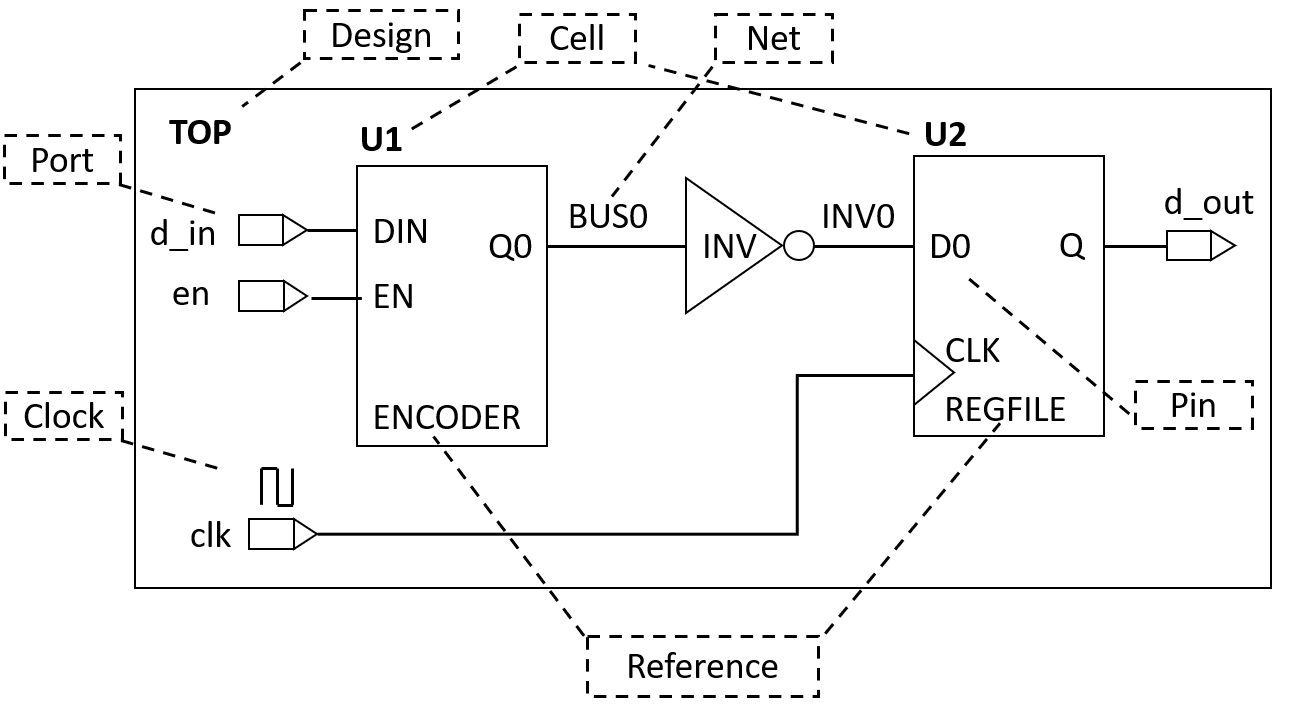
\includegraphics[width=0.5\linewidth]{assets/16/DC处理对象划分.png}
  \caption{DC处理对象划分}
  \label{fig:dc-obj}
\end{figure}

逻辑综合通常包括translation、optimization和mapping三个步骤：

\begin{itemize}
\tightlist
\item
  translation：将HDL描述的电路转换为用GTECH库元件组成的逻辑电路，GTECH库是synopsys的通用工艺库，仅表示逻辑函数的功能，并没有映射到具体的厂家工艺库。
\item
  optimization：在这一步骤中，逻辑综合工具会根据设计指标（如时序、面积、功耗等）对转译后的数据库进行优化。优化过程可能会去除一些被认为是``无用的模块''，如未连接的端口或永远不会触发的状态机跳转条件。
\item
  mapping：将优化后的电路转换为目标工艺库对应的门级网表。它确保了电路能够在特定的工艺条件下实现。
\end{itemize}

如图\ref{fig:dc-flow}是Synopsys DC综合工作流程示意图：

\begin{figure}[htbp]
  \centering
  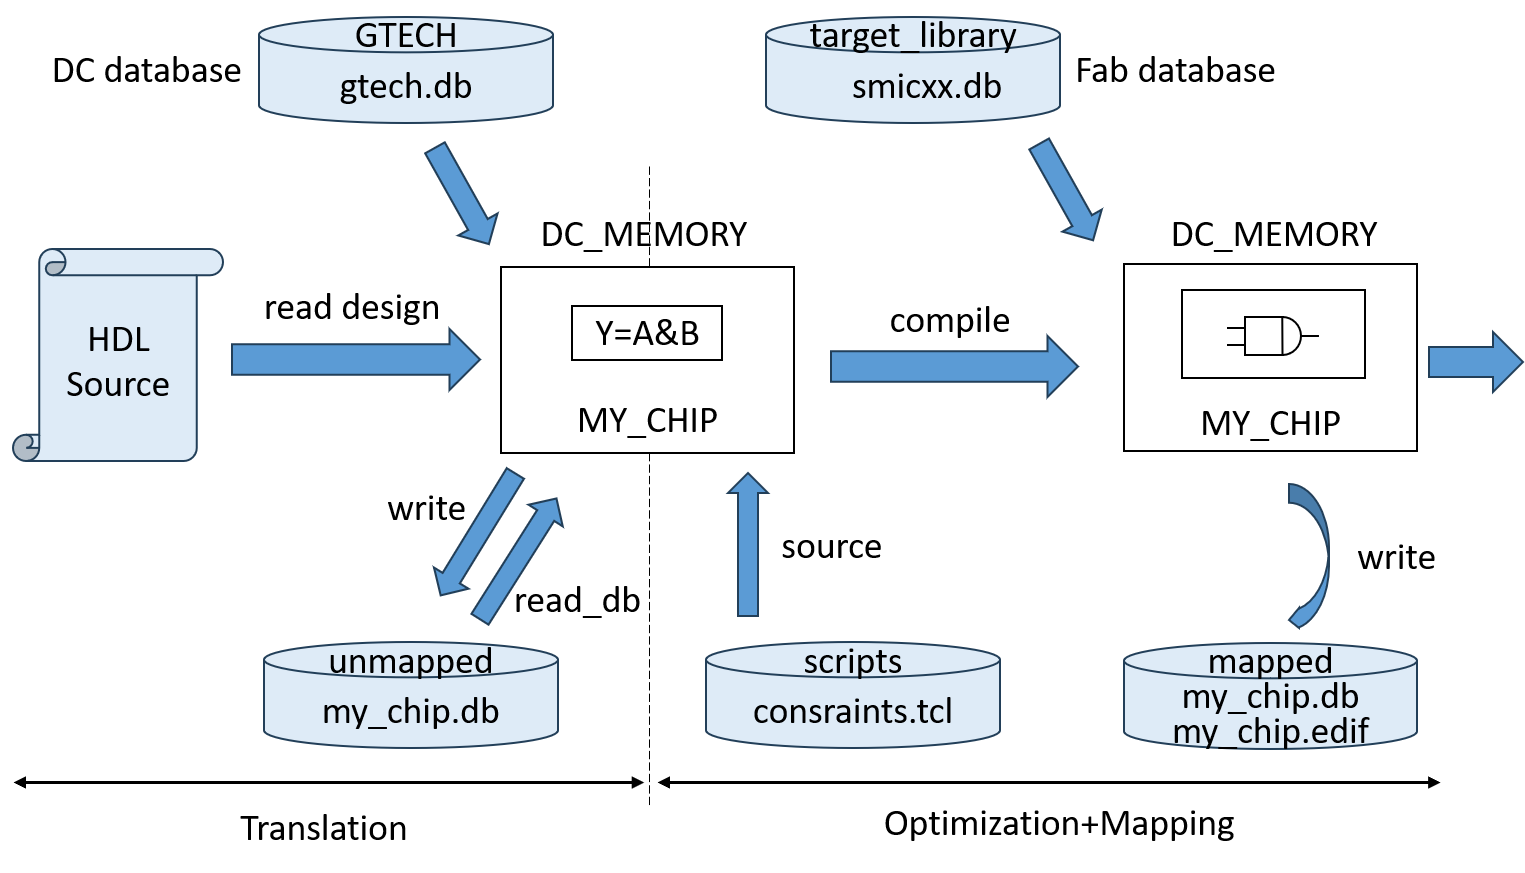
\includegraphics[width=0.5\linewidth]{assets/16/DC综合过程示意图.png}
  \caption{DC综合过程示意图}
  \label{fig:dc-flow}
\end{figure}

\subsection{逻辑综合实施流程}\label{sec:16-chip-frontend-020}

逻辑综合的具体实现流程如图\ref{fig:dc-workflow}所示，包含指定工艺库、读入设计、定义设计环境、设计约束、设计规则约束、优化约束、编译策略选择、分析报告、写文件等过程。下面将针对每一步的设置进行展开描述。

\begin{figure}[htbp]
  \centering
  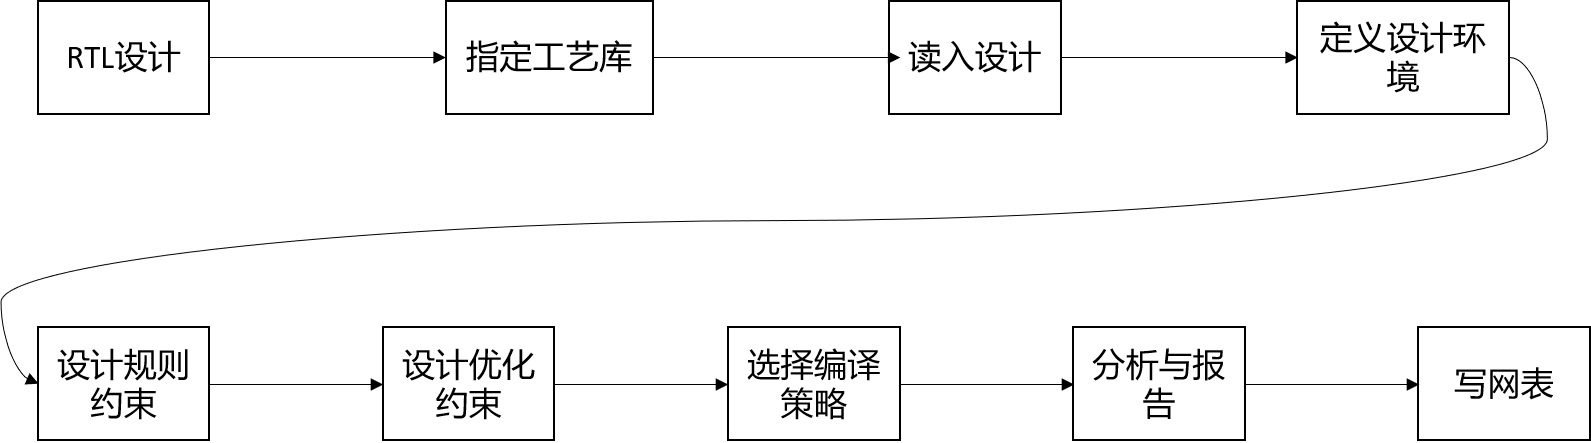
\includegraphics[width=0.5\linewidth]{assets/16/DC工作流程.png}
  \caption{DC工作流程}
  \label{fig:dc-workflow}
\end{figure}

\begin{itemize}
\item
  1.设计实现HDL文件：即在综合开始前需要准备好设计完善的可综合RTL文件。
\item
  2.指定库文件：库文件包括链接库（Link library）、目标库（target
  library）、符号库（symbol library）、综合库（synthetic
  library）。其中链接库与目标库是必须指定的，这两者也被称为工艺库，二者可以使用一个库文件。下面对这几种库文件进行描述：

  \begin{itemize}
  \tightlist
  \item
    链接库：用于指定综合工具在解析设计时用来解析逻辑单元的库。这些库文件包含了设计中的所有单元（如门、触发器、宏单元等）的定义。它确保综合过程中引用的所有单元都能被正确解析并链接。
  \item
    目标库：用于指定综合过程中实际进行逻辑映射和优化所使用的库。这些库文件提供了目标单元的时序、功耗、面积等详细信息，Design
    Compiler 将设计映射到这些单元上，并根据它们的特性进行优化。
  \item
    符号库：提供 Design Vision GUI
    中设计实现的图形符号，如果使用脚本模式而不使用
    GUI,此库可不指定。
  \item
    综合库：亦称为 Designware
    库，尽管其名称翻译为``综合库''，但通常被称为 IP 库。某些特殊的
    Designware
    库（例如多级流水线乘法器）需要获得授权许可。然而，默认的标准
    Designware 库由 Design Compiler
    软件供应商直接提供，无需用户额外指定。
  \end{itemize}

  需要注意的是当读入的文件是门级网表时，需要把 link library
  指向生成该门级网表的库文件，否则 DC
  因不知道网表中门单元电路的功能而报错。

  一般设置脚本为：

% 代码语言：BookTcl
\begin{CodeBlock}[language=BookTcl]
set link_library [list "std_cells.db" "macros.db" "black_boxes.db"]
set target_library [list "std_cells.db"]
set symbol_library [list "sym.db"]
set synthetic_library [list "dw_foundation.sldb"]
\end{CodeBlock}
\item
  3.读入设计：设计的读取过程包括将设计文件加载到内存中，并将其转换为
  DC 的中间格式，即 GTECH 格式。GTECH 格式由 `soft macros'
  组成，如加法器、比较器等，这些组件来源于 Synopsys
  的合成库，每种组件有多种不同的结构。读入设计有两种实现方式：

  \begin{itemize}
  \tightlist
  \item
    read\_verilog/read\_vhdl
  \item
    analyze \& elaborate
  \end{itemize}

  第二种读取方式可以自由指定设计库，并在生成GTECH中间文件前生成.syn文件存储于work目录下。这样可以在下次elaborate时节省时间。我们在读取RTL设计时一般选用第二种方法读取。下面是一个使用脚本，其中RTL\_SRC定义了所有源文件路径，ACTIVE\_DESIGN是顶层模块的名称。
\end{itemize}

% 代码语言：BookTcl
\begin{CodeBlock}[language=BookTcl]
analyze -format sverilog $RTL_SRC
elaborate $ACTIVE_DESIGN
link
uniquify
check_design > ./check_design.log
\end{CodeBlock}

\begin{itemize}
\item
  4.定义设计环境：具体包括工艺库的工艺电压温度（PVT）条件、线负载模型、IO端口属性（驱动、扇出、负载等），这些设计环境会影响综合及优化结果。下面给出一些常用命令：

  \begin{itemize}
  \item
    set\_operating\_conditions:指定不同的分析类型（如最坏情况、最好情况或基于芯片变异性的分析），并可以选择不同的库文件（如最慢库、典型库、最快库）来适应不同的分析需求。此外，该指令还可以与其他SDC（Synopsys
    Design
    Constraints）命令结合使用，以更精确地控制设计的时序和功耗特性。
  \item
    set\_driving\_cell/set\_drive/set\_input\_transition：三个命令都会影响输入端口驱动强度。我们通过set\_driving\_cell命令来设置某个输入端口前面是什么驱动单元驱动它的，EDA工具会从指定的库中查找得出更加真实的Transition时间来代替零Transition。set\_drive命令通过为输入端口指定电阻值的方法来为其定义外部驱动强度。在逻辑综合工具进行优化期间，工具根据设置的驱动强度来计算由该输入端口驱动的逻辑电路的延迟。set\_input\_transition命令为输入端口指定一个固定的transition时间，工具会用该transition时间来计算它驱动的逻辑电路的延迟。
  \item
    set\_wire\_load\_model：指定估算线延迟时所选用的模型。包含zero wire
    load model、基于fanout的传统WLM以及基于物理位置的wire load
    model。
  \end{itemize}
\item
  5.设计约束：包括设计规则约束与优化约束。设计规则约束（DRC）由工艺库决定，包括最大转换时间、最大扇出以及最大电容。优化约束就包括关键的时钟约束、输入输出延时以及面积约束等。DC会根据这个优化约束条件来权衡综合出的网表，使之尽量满足约束条件。下面是一些常用的脚本命令：
\end{itemize}

% 代码语言：BookTcl
\begin{CodeBlock}[language=BookTcl]
# 设置最大信号转换时间  
set_max_transition 0.5 -net [get_nets clk_net]  
# 解释：为名为clk_net的网络设置最大信号转换时间为0.5纳秒。这有助于控制信号完整性
  
# 设置最大扇出数  
set_max_fanout 10 -cell BUF_X1  
# 解释：为单元BUF_X1设置最大扇出数为10。这有助于防止由于过多负载而导致的性能下降
  
# 注意：有些工具可能不支持直接为单元设置最大扇出数，而是需要设置最大负载电容等
  
# 设置最大电容值  
set_max_capacitance 0.1 -net data_net  
# 解释：为名为data_net的网络设置最大电容值为0.1皮法。这有助于控制信号延迟和功耗
  
# 创建时钟  
create_clock -name clk -period 10 -waveform {0 5} [get_ports clk_port]  
# 解释：创建一个名为clk的时钟，周期为10纳秒，波形为占空比50%（从0到5纳秒为高电平），并将其
# 与名为clk_port的端口相关联  
  
# 设置时钟延迟  
set_clock_latency 1.0 -source -max [get_clocks clk]  
# 解释：为名为clk的时钟设置源端最大延迟为1.0纳秒。这考虑了时钟源到设计中各点的传播延迟
  
# 设置传播时钟  
set_propagated_clock [get_clocks -of [get_cells buf_inst]]  
# 解释：这通常不是直接设置的命令，而是用于识别和传播时钟的。上面的命令是假设性的，具体取决
# 于工具如何自动处理时钟的传播  
  
# 设置时钟不确定性  
set_clock_uncertainty 0.2 -setup [get_clocks clk]  
# 解释：为名为clk的时钟设置建立时间不确定性为0.2纳秒。这考虑了时钟抖动和其他不确定因素
  
# 设置时钟转换时间  
set_clock_transition 0.3 -clock clk  
# 解释：为名为clk的时钟设置最大转换时间为0.3纳秒。这有助于控制时钟信号的完整性
  
# 设置输入延迟  
set_input_delay -clock clk -max 2.0 [get_ports data_in]  
# 解释：为名为data_in的输入端口设置相对于名为clk的时钟的最大输入延迟为2.0纳秒
#（用于建立时间分析）  
  
# 设置输出延迟  
set_output_delay -clock clk -max 2.5 [get_ports data_out]  
# 解释：为名为data_out的输出端口设置相对于名为clk的时钟的最大输出延迟为2.5纳秒
#（用于保持时间分析）  
  
# 注意：设置最大面积（set_max_area）通常不是时序分析的一部分，而是优化或物理实现阶段可能考虑的约束  
# 假设存在一个设置面积约束的命令，它可能看起来像这样（但具体取决于工具）：  
# set_max_area 1000000 -design my_design  
# 解释：为名为my_design的设计设置最大面积为1000000平方微米
\end{CodeBlock}

\begin{itemize}
\item
  6.选择编译策略：两种编译策略：Top-down与Bottom-up；这两种策略侧重点有所不同：

  \begin{itemize}
  \tightlist
  \item
    Top-down（自顶向下）：适用于小型或中等规模设计，因为这种策略可以再整个设计中应用统一的约束和优化。
  \item
    Bottom-up（自底向上）：适用于大型或非常复杂的设计，因为这种策略运算分阶段编译和优化。
  \end{itemize}

  在使用命令编译时，直接输入compile或compile\_ultra即可编译（是一个更高级的综合命令，用于执行更深层次的优化。它在综合过程中使用了更激进的优化策略，以获得更好的时序、功耗和面积优化）。
\item
  7.分析与报告：report面积（资源）、时序、功耗等信息，查看时序是否收敛、面积是否查出目标范围等。对于设计中存在的问题可以使用check\_design命令来检查。
\item
  8.写网表等文件：在DC结束编译后，可以通过下述命令来实现写网表文件（除了.v格式还有DC支持的.ddc格式）：
\end{itemize}

% 代码语言：BookTcl
\begin{CodeBlock}[language=BookTcl]
write -format verilog -hierarchical -output your_design_synth.v
write -format ddc -hierarchical -output your_design_synth.ddc
\end{CodeBlock}

\section{静态时序分析}\label{sec:16-chip-frontend-021}

静态时序分析（Static Timing Analysis,
STA）是数字集成电路设计中关键的验证步骤，用于确保设计在指定的工作频率下满足所有时序约束。相比动态仿真，STA不依赖特定的输入激励，而是通过分析电路中所有可能的时序路径来验证设计的时序完整性，从而在较短时间内覆盖整个电路。

\subsection{时序路径与基本概念}\label{sec:16-chip-frontend-022}

\begin{itemize}
\item
  时序路径：STA中，路径通常由起点（如触发器的输出端）、组合逻辑电路、和终点（如另一个触发器的输入端）组成。STA分析中，有四种时序路径：

  \begin{itemize}
  \tightlist
  \item
    输入端口到触发器的输入端
  \item
    输入端口到输出端口
  \item
    触发器的时钟到另一个触发器的输入端
  \item
    触发器的时钟到输出端口
  \end{itemize}
\item
  时钟域：时钟域是电路中受同一时钟信号控制的部分。在不同的时钟域之间传递信号可能会引发跨时钟域的问题，因此需要特别关注。
\item
  建立时间（setup）和保持时间（hold）：寄存器对输入信号的要求，即信号必须在时钟边沿前保持稳定（建立时间）并在之后维持一段时间（保持时间）才能被正确采样。如图\ref{fig:setup-hold}所示为概念图。

  \begin{itemize}
  \tightlist
  \item
    建立时间（setup
    time）：寄存器在时钟上升沿到达前应当保持数据不变的时间。
  \item
    保持时间（hold
    time）：寄存器时钟上升沿到达后数据应当继续保持的最短时间。
  \end{itemize}
\end{itemize}

\begin{figure}[htbp]
  \centering
  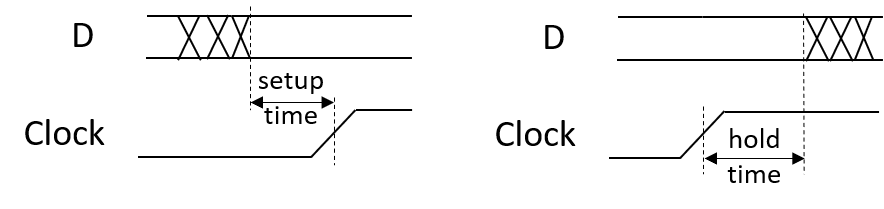
\includegraphics[width=0.5\linewidth]{assets/16/建立时间与保持时间概念.png}
  \caption{建立时间与保持时间}
  \label{fig:setup-hold}
\end{figure}

\subsection{静态时序分析的核心步骤}\label{sec:16-chip-frontend-023}

时钟树综合（Clock Tree Synthesis,
CTS）：生成并优化电路中的时钟树，确保时钟信号在所有寄存器中同步到达。时钟树的设计和优化对时序分析的准确性至关重要。

时序约束设置：使用SDC（Synopsys Design
Constraints）文件定义设计的时序约束，包括时钟定义、输入输出延迟、时钟不确定性等。合理的约束设置是STA成功的基础。

路径延迟计算：STA工具通过计算时序路径中的信号传播延迟，包括组合逻辑延迟、寄生效应引起的延迟和时钟延迟，来确定路径是否满足时序约束。

时序违规检测：STA工具会检测是否存在路径延迟超过时钟周期导致的时序违规，并报告潜在的建立时间和保持时间问题。

\subsection{STA中的关键问题}\label{sec:16-chip-frontend-024}

时钟偏斜（Clock
Skew）：由于时钟网络中不同寄存器的时钟到达时间不同，可能引发时序违规。优化时钟偏斜是确保时序正确性的关键。

时钟不确定性（Clock
Uncertainty）：制造工艺差异、温度变化和电源噪声可能导致时钟信号不确定性。STA中需要考虑时钟不确定性，确保时序裕量充足。

多周期路径（Multicycle Paths,
MCP）：一些时序路径需要多个时钟周期才能完成信号传播。STA工具必须正确识别这些路径，避免错误报告时序违规。

假路径（False
Paths）：由于设计原因不会被实际激活的路径应标识为假路径，以防止它们在STA中引发虚假时序违规。

跨时钟域路径（Cross-Clock Domain
Paths）：信号跨越不同时钟域时可能产生时序问题，通常通过同步器或异步FIFO处理。

\subsection{时序优化与收敛}\label{sec:16-chip-frontend-025}

逻辑优化：如果发现时序违规，可以通过重构逻辑路径、减少逻辑级数或插入缓冲器来优化电路。

时钟树优化：通过减少时钟偏斜和抖动来优化时钟树，确保时钟信号在电路中同步分布。

寄生效应优化：调整布局布线以减少寄生电容和电阻对信号延迟的影响，进而改善时序性能。

时序裕量增加：在必要时调整时钟频率或增加时钟周期，确保时序路径有足够的裕量来应对工艺波动和环境变化。

\subsection{STA工具与分析流程}\label{sec:16-chip-frontend-026}

STA工具（如Synopsys
PrimeTime）通过详细的路径分析和时序报告，帮助设计者识别时序问题并提供优化建议。STA流程通常贯穿设计的多个阶段，包括综合后、布局布线后和签核前的最终分析，每个阶段都需要验证时序完整性。下面给出PrimeTime的一个约束脚本模板：

% 代码语言：BookTcl
\begin{CodeBlock}[language=BookTcl]
# 设置时钟约束
create_clock -period 10 [get_ports clk]
set_clock_uncertainty 0.5 [get_clocks clk]
set_clock_latency 1.2 [get_clocks clk]

# 设置输入延迟约束
set_input_delay -max 2.5 -clock clk [get_ports in_port]
set_input_delay -min 1.5 -clock clk [get_ports in_port]

# 设置输出延迟约束
set_output_delay -max 3.0 -clock clk [get_ports out_port]
set_output_delay -min 2.0 -clock clk [get_ports out_port]

# 设置伪路径约束（如果有需要）
set_false_path -from [get_ports start_signal] -to [get_ports end_signal]

# 设置多周期路径约束（如果有需要）
set_multicycle_path 2 -from [get_ports source_port] -to [get_ports destination_port]
\end{CodeBlock}

一般STA除了在最终signoff阶段进行外，还要在芯片设计中的多个环节进行，确保每一步的设计都满足时序的要求：

\begin{itemize}
\item
  1.逻辑综合后的STA：逻辑综合（Synthesis）完成后，STA用于验证综合结果是否满足时序要求。这个阶段的STA主要关注：

  \begin{itemize}
  \tightlist
  \item
    综合后的时序验证：确保逻辑综合后的电路在目标频率下能够满足时序约束。
  \item
    时钟和数据路径分析：检查数据路径和时钟路径是否满足设置的时序约束，发现潜在的时序违例。
  \end{itemize}
\item
  2.布局规划后的STA：布局规划（Placement）完成后，STA再次进行，以评估布局对时序的影响。这个阶段的STA主要关注：

  \begin{itemize}
  \tightlist
  \item
    布置后的时序验证：确保布局后的电路在实际布线之前满足时序要求。
  \item
    时钟树综合（CTS）后的时序分析：
    检查时钟树综合后的时钟路径，确保时钟分布和信号到达时间符合设计要求。
  \end{itemize}
\item
  3.布线后的STA：布线（Routing）完成后，STA是必须的，因为布线阶段可能引入新的延迟和时序问题。这个阶段的STA主要关注：

  \begin{itemize}
  \tightlist
  \item
    布线后的时序验证：确保布线后的设计满足所有时序约束，包括时钟周期、数据传输延迟等。
  \item
    时序优化：针对布线阶段发现的时序问题进行优化，可能需要重新调整布局或布线，以解决时序违例。
  \end{itemize}
\item
  4.功耗优化和时序优化后的STA：在功耗优化和时序优化阶段后，STA需要进行，以验证优化措施对时序的影响。这个阶段的STA主要关注：

  \begin{itemize}
  \tightlist
  \item
    优化后的时序验证：确保在进行功耗和时序优化后，设计依然满足时序要求。
  \item
    验证优化效果：确认优化措施是否有效，是否解决了之前发现的时序问题。
  \end{itemize}
\item
  5.设计验证的最后阶段（Signoff）：最终签核（Signoff）
  阶段是STA的关键环节。此时，设计团队会进行全面的时序验证，确保所有的时序要求和约束都已满足。这通常包括：

  \begin{itemize}
  \tightlist
  \item
    全设计时序签核：对整个设计进行全面的时序分析，确保在各种工作条件下（例如不同的工艺角、电源电压、温度等）满足时序要求。
  \item
    签核报告：生成时序签核报告，记录所有分析结果和任何可能的违例，作为最终验证的依据。
  \end{itemize}
\end{itemize}

\section{芯片可测性设计}\label{sec:16-chip-frontend-027}

芯片可测试性设计是指在不影响芯片正常功能的前提下在芯片中加入有利芯片测试的电路结构，即有利于芯片测试的辅助性设计，芯片可测试性设计是数字集成电路设计流程中的重要环节，对有效提升芯片的测试效率，降低芯片的测试成本有重要的意义。

主要的可测性设计方法包括：扫描测试、内建自测试等。

\subsection{扫描测试}\label{sec:16-chip-frontend-028}

\subsubsection{扫描链}\label{sec:16-chip-frontend-029}

\begin{itemize}
\tightlist
\item
  难点及应用
\end{itemize}

对于现代数字系统的测试，由于设计规模较大，难以直接获取电路内部节点的值，因此如果采取直接测试的方式，在设计输入处施加激励，输出端进行观察，难以对电路内部故障进行定位和诊断；并且现代数字系统几乎都是时序逻辑电路，对于时序逻辑电路而言，电路一旦发生故障，可能会经过许多个周期才会在输出端体现出来，甚至会在传播途中消失，而对组合逻辑进行测试，电路的故障则会立即在输出端体现。因此扫描链的重要性显现出来。

\begin{itemize}
\tightlist
\item
  扫描链原理
\end{itemize}

扫描链，即Scan
Chain，由扫描单元前后相接而成，扫描单元又叫扫描触发器，通过在触发器的D端增加选择器(MUX)，增加扫描输入端口，扫描输出端口以及扫描使能端口，形成扫描单元，前一个扫描单元的扫描输出与后一个扫描单元的扫描输入相接形成链，如图\ref{fig:dft-scan-chain}所示，MUX的另一端与电路中的组合逻辑相连接，允许通过扫描使能端口控制触发器的D端来自扫描输入或者组合逻辑。

\begin{figure}[htbp]
  \centering
  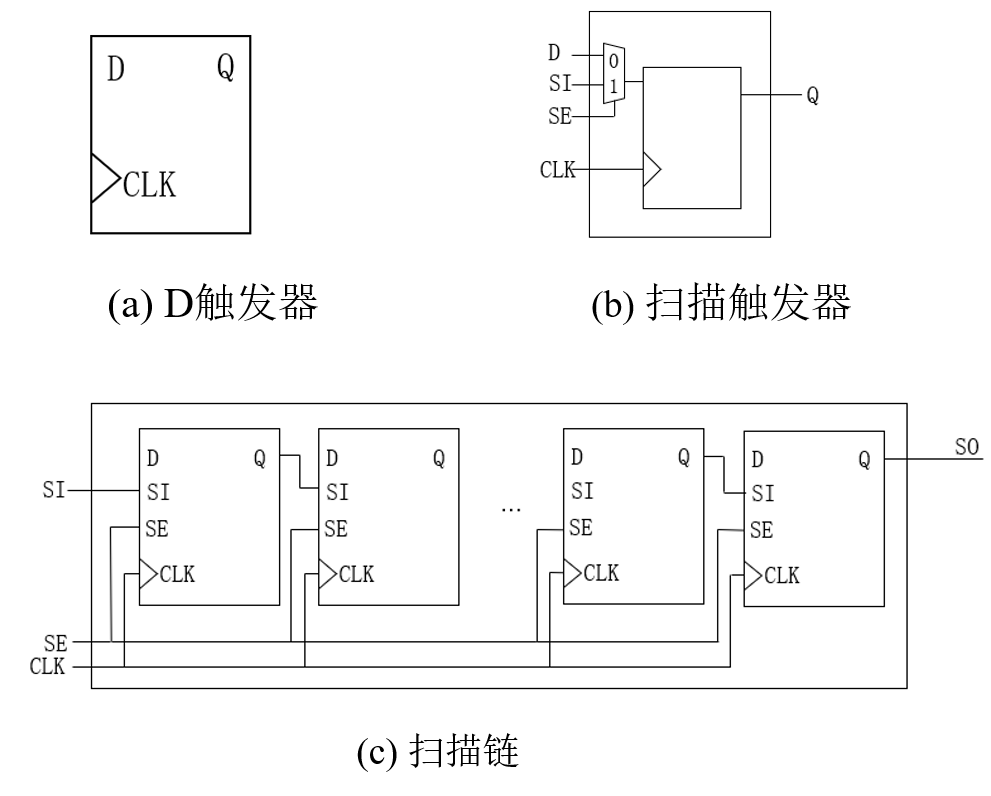
\includegraphics[width=0.5\linewidth]{assets/16/DFT扫描链.png}
  \caption{DFT扫描链}
  \label{fig:dft-scan-chain}
\end{figure}

\begin{itemize}
\tightlist
\item
  扫描链优缺点
\end{itemize}

当扫描使能信号为高时，扫描单元从扫描输入获取数据，此时扫描链构成移位寄存器，可通过扫描输入端口串行输入测试数据。在实际测试中，先将扫描使能信号端口拉高，经扫描输入端口进行测试数据移位输入；再拉低扫描使能信号端口，此时扫描单元的输入与输出均为电路中的组合逻辑，移位输入的值进入组合逻辑完成赋值并运算，在功能端口实现电路输出；之后再次拉高扫描使能信号，此时电路组合逻辑内部节点的运算结果进入扫描单元，通过移位串行输出内部节点值，以便与预期值比较，判断电路内部是否故障。扫描输入和预期输出值通常由工具自动生成，在测试向量自动生成流程中完成。

扫描链可将难以测试的时序逻辑电路转化为易测的组合逻辑电路，能有效提高电路的可测试性与可观察性，但会增加额外硬件面积，一定程度上提升了设计复杂性。

\subsubsection{测试向量自动生成}\label{sec:16-chip-frontend-030}

\begin{itemize}
\tightlist
\item
  ATPG原因
\end{itemize}

测试向量自动生成（ATPG）通过抽象电路故障模型，运用推导算法得出测试向量。现代数字系统发展迅速，测试难度大，其自动化测试数据也纳入自动化流程。借助
EDA 算法和计算机技术，自动化测试数据产生工具简化测试流程，现代 EDA
工具抽象故障、运用算法高效产生测试数据，与其他 EDA
工具配合构建全流程自动化测试体系。

\begin{itemize}
\tightlist
\item
  电路故障模型
\end{itemize}

电路故障模型主要有固定型故障、开 /
短路故障、传输延时故障等。固定型故障是目前主要且最早使用的故障类型，指电路某点信号锁定在
0 或 1
状态致电路错误，可检测大部分工艺失效，其不同位置的信号锁定在特殊情况下可等效，故在等效故障集合中选一个进行测试向量推导即可。固定开
/ 短路故障是电路中某晶体管状态固定致电路错误。传输延时故障指电路中某点
01
翻转过慢或某路径延迟过大，可能致电路时序出错，检测时需先通过一条测试向量将故障点置
0 或 1，再用另一条向量置相反值以检测节点能否在相应时间内完成翻转。

\begin{itemize}
\tightlist
\item
  测试向量中的推导算法
\end{itemize}

对电路各类故障类型抽象后，可采用不同算法推导测试向量。其中经典的 D
算法主要有几个步骤：首先是传播，确定检测某处故障后，将故障影响向输出端传递以推导期望输出；为激活故障需进行合理化，即推导其他节点的值；合理化过程中若节点值发生冲突，则需回溯至上一节点进行推导。现代各种测试向量算法多是
D 算法的优化和迭代。现代 EDA 工具可较快完成 ATPG
过程，在软件层面推导测试向量。由 ATPG 得到测试向量后，可使用
ATE（自动化测试设备）对芯片进行检测。

\begin{itemize}
\tightlist
\item
  ATPG优势以及一般要求
\end{itemize}

ATPG 优势明显。在现代 EDA
工具助力下，流程自动快捷，可大幅减少测试向量集，以最小成本实现最大测试效率。完成测试向量推导后，用故障覆盖率指标评判质量。测试覆盖率是扫描测试重要指标，由可检测故障数与故障总数比值计算，反映对设计故障的覆盖情况。一般设计的
ATPG 测试覆盖率要达 90\% 以上，航天、自动驾驶等领域要求更高，需达 99\%。

\subsubsection{自动化测试设备}\label{sec:16-chip-frontend-031}

自动化测试设备（ATE）是高度发达的测试系统，由软件系统和硬件系统组成。硬件系统包含测试通道（对应不同存储深度且有各自测试图形发生器）、时钟单元及
PCI
接口用于数据交换；软件系统包括测试图形编辑单元、设计工程接口及待测电路接口。

ATE
价格昂贵，由测试时间和总线位宽决定，时间越长、位宽越大，成本越高。为减少成本，常对多个芯片并行测试。随芯片复杂程度增高，测试图形复杂庞大，ATE
机台可能需多次加载完成测试图形载入，导致测试时间长、成本飙升，故需减小测试向量数目和大小，现代
EDA 工具一般通过压缩扫描链实现此目的。

\subsubsection{扫描链压缩}\label{sec:16-chip-frontend-032}

\begin{itemize}
\item
  压缩的重要性：扫描链压缩是在设计规模较大、扫描单元数量过多时采取的策略。若扫描链长度过大，会导致测试向量过大，可能超出
  ATE
  机台存储容量，需多次加载，增加测试时间；若减少扫描链长度，则数量增多，需较多额外端口作为测试端口，加大端口分配压力，甚至可能超过
  ATE
  机台限度，使芯片无法正常测试。因此，扫描链压缩对设计规模大、扫描单元数量多的情况意义重大。本文对加入的扫描链进行了压缩操作。
\item
  压缩原理：扫描链压缩在扫描链输入和输出端口增加额外逻辑，对测试向量进行压缩和解压缩。不同现代
  EDA 工具方式不同，如 Synopsys
  旗下工具解压缩逻辑是可编程广播式传播，压缩逻辑是异或树；Mentor
  旗下工具解压缩逻辑是环形测试向量生成器，压缩逻辑基于片上多输入签名寄存器。虽实现方式不同，但都能有效压缩测试向量，减少测试成本。扫描测试系统时钟由片上时钟控制器控制。
\item
  扫描链压缩优缺点：扫描链压缩可以有效解决设计规模较大导致扫描链数目和长度难以权衡的问题，代价是需要增加额外的逻辑，占用了额外的面积，但是在可以接收的范围内，因此扫描链压缩广泛使用在扫描测试中。
\end{itemize}

\subsubsection{片上时钟控制器}\label{sec:16-chip-frontend-033}

片上时钟控制器（OCC）在扫描测试中用于控制测试时钟。芯片处于功能模式时，OCC
输出内部时钟；处于测试模式时，输出来自 ATE
机台的慢速测试时钟，并可旁路内部时钟，实现功能模式与测试模式切换。若不选择测试时钟，测试机台对测试过程可控性下降且易受内部时钟干扰，问题难定位。加入
OCC 后，ATPG 工具能更有效追踪扫描链。OCC 一般位于 PLL 之后，输入 PLL
生成的快速时钟和 ATE
的慢速时钟，在不同模式下由控制信号选通不同时钟源。加入 OCC
后会生成时钟链，与扫描链不同，OCC
需要额外端口控制，会带来一定测试端口和电路面积开销。

\subsection{内建自测试}\label{sec:16-chip-frontend-034}

内建自测试（Built In Self
Test，BIST）是在芯片内部自动测试的技术，存储器的故障模式相对较为明确，且对存储器进行全面测试较为困难，所以内建自测试在存储器测试中广泛应用。存储器内建自测试（Memory
Built-in Self
Test，MBIST）即在存储芯片内部引入测试向量生成模块和测试向量检测及压缩模块，可以有效对电路内部的缺陷进行检测，不依赖于昂贵的ATE设备，如图\ref{fig:MBIST}。

\begin{figure}[htbp]
  \centering
  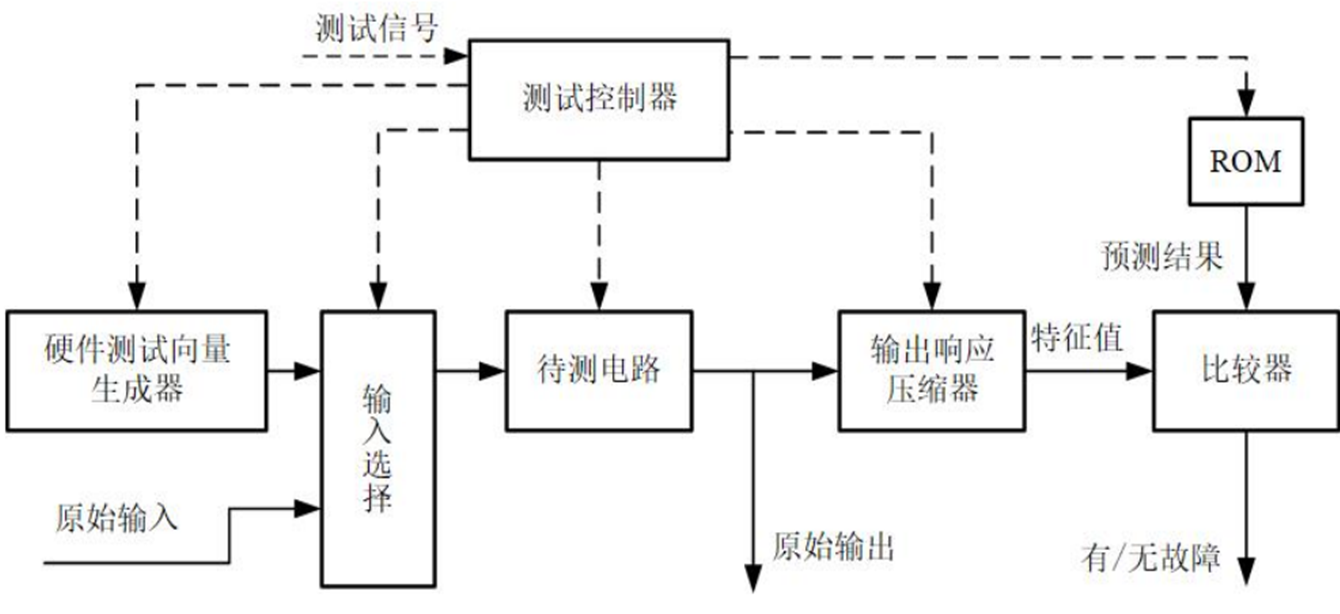
\includegraphics[width=0.5\linewidth]{assets/16/内建自测试电路模块示意图.png}
  \caption{内建自测试模块示意图}
  \label{fig:MBIST}
\end{figure}

\subsubsection{存储器故障类型}\label{sec:16-chip-frontend-035}

存储器主要包括地址解码，存储和读写控制单元，主要故障类型包括单元固定故障，状态跳变故障，单元耦合故障等类型。单元固定故障，即Stuck
At Fault，是指存储器单元固定在0或者1状态；状态跳变故障，即Transition
Delay
Fault，是指对存储器进行读写操作时，存储器状态跳变异常；单元耦合故障是，即Coupling
Fault，指当存储器单元发生状态跳变时，会对其周围存储器单元造成影响，该种故障类型主要针对RAM。针对不同类型的故障，需要不同的测试激励进行检测。例如要检测单元固定故障，则需要对可能存在故障的单元进行数据0/1的读写。

\subsubsection{存储器测试算法}\label{sec:16-chip-frontend-036}

对存储器的测试算法主要包括棋盘式图形算法和March算法。其中棋盘式图形算法通过对相邻存储器进行分组，向不同组写入01交替的测试向量，之后对存储器进行读取操作，可以检测某些存储器故障。March算法在目前广泛使用，对不同单元进行依次操作，March算法中的操作单元称为March单元，由各种不同的操作序列组成，March算法有不同变体，对故障类型的覆盖各有差异，覆盖率也有所不同。

% !TeX root = ../main.tex
% 原始章节：17-chip-backend.Rmd

\chapter{芯片后端实现}\label{chap:17-chip-backend}

本章内容将根据后端流程、物理实现（布局布线等）、时序signoff（静态时序分析）、功耗与IR signoff、物理验证五个部分进行描述。

\section{芯片后端设计流程}\label{sec:17-chip-backend-001}

芯片后端设计流程是芯片设计过程中至关重要的环节，它涵盖了从前端设计完成后的电路布局、布线、物理实现及验证的全部工作。

芯片后端设计流程主要包括以下几个阶段：

\begin{itemize}
\tightlist
\item
  设计规划：这个阶段一般在芯片项目初期完成，明确芯片合适的工艺节点、性能、面积功耗范围等。同时，还需要制定详细的项目计划和时间表。
\item
  逻辑综合：如第16.5节所述，逻辑综合是将高级语言描述的逻辑设计转化为门级网表的过程，生成的门级网表将作为后续布局布线的输入（这一步也可以认为是前端综合的工作）。
\item
  \textbf{布局规划}：布局规划是芯片后端设计的重要环节，它决定了芯片中各个元件的位置和布局。在这个阶段，需要考虑芯片的尺寸规划、IO 规划、macro 摆放、物理单元插入等因素。合理的布局规划可以提高芯片的性能、降低功耗、减小面积。

  \begin{itemize}
  \tightlist
  \item
    芯片尺寸规划：芯片尺寸规划需要根据芯片的功能需求和性能指标来确定。一般来说，芯片尺寸越大，能够容纳的元件越多，但成本也会相应增加。在进行芯片尺寸规划时，需要考虑到工艺节点、封装形式、散热要求等因素。
  \item
    IO 规划：IO 规划是确定芯片输入输出端口的位置和数量。合理的 IO 规划可以提高芯片的易用性和可靠性。在进行 IO 规划时，需要考虑到信号完整性、电源完整性、封装要求等因素。
  \item
    Macro 摆放：Macro 摆放是将宏单元（如存储器、处理器核等）放置在芯片中的合适位置。Macro 的摆放需要考虑到信号传输的路径、功耗分布、散热要求等因素。
  \item
    物理单元插入：物理单元插入是在芯片中插入一些特殊的物理单元，如电源网格、时钟树单元等，以提高芯片的性能和可靠性。在进行物理单元插入时，需要考虑到工艺节点、设计约束、信号完整性等因素。
  \end{itemize}
\item
  \textbf{时钟树综合}：时钟树综合是构建时钟信号的传输网络，确保时钟信号的准确性和稳定性。时钟树综合的基本步骤包括确定时钟源和时钟目标、设计时钟树结构、调整时钟树的延迟和偏差等。
\item
  \textbf{布线}：布线是连接芯片中的各个元件，实现信号的传输。布线的基本步骤包括全局布线、详细布线、布线优化等。
\item
  \textbf{物理验证}：物理验证是检查芯片的设计是否符合制造工艺的要求，如 DRC（设计规则检查）、LVS（版图与原理图一致性检查）、Antenna 检查等。物理验证的目的是确保芯片的设计能够在制造过程中顺利实现，并且具有良好的性能和可靠性。
\item
  \textbf{时序分析}：时序分析是分析芯片的时序性能，确保满足设计要求。时序分析的基本步骤包括提取时序模型、进行静态时序分析（STA）、修复时序违规等。在物理实现的各个阶段以及最终的signoff，STA都需要进行以确保每一步的时序都满足要求。
\item
  \textbf{功耗分析}：功耗分析是评估芯片的功耗，进行优化以降低功耗。功耗分析的基本步骤包括功耗建模、功耗评估、功耗优化等。合理的功耗分析可以降低芯片的功耗，提高芯片的可靠性和稳定性。
\item
  \textbf{最终输出}：最终输出是生成用于制造芯片的 GDSII 文件。GDSII 文件包含了芯片的物理信息，如元件的位置、形状、连接关系等。在生成 GDSII 文件之前，需要进行最后的检查和验证，确保芯片的设计符合制造工艺的要求。
\end{itemize}

\section{芯片物理设计}\label{sec:17-chip-backend-002}

\subsection{设计初始化}\label{sec:17-chip-backend-003}

后端设计需要的库文件主要包括工艺库、IP库和设计约束文件等。 工艺库提供了制造芯片所需的各种物理信息，如晶体管的尺寸、电容电阻值、工艺规则等。工艺库是芯片物理设计的基础，它涵盖了芯片的性能、功耗、面积等关键信息。

IP库包含了预先设计好的功能模块，可以直接在设计中使用。IP库可以提高芯片设计的效率和质量，减少设计时间和成本。例如，IP库中的存储器等模块可以直接集成到芯片设计中，无需重新设计。

设计约束文件则规定了芯片的性能要求，如时序约束、面积约束、功耗约束等。设计约束文件是芯片物理设计的指导，它决定了芯片的设计方向和优化目标。例如，设计约束文件中的时序约束规定了芯片中各个信号的传输时间和延迟要求，设计人员需要根据这些约束进行布局布线和时序优化，以确保芯片的时序性能满足设计要求。

以 Innovus 为例，数据初始化的步骤如下：

\begin{itemize}
\item
  导入工艺库和设计约束文件。在 Innovus 中，可以通过菜单栏中的 ``File''-\textgreater{}``Import''-\textgreater{}``Library'' 和 ``File''-\textgreater{}``Import''-\textgreater{}``Constraints'' 分别导入工艺库和设计约束文件。
\item
  创建设计项目，设置芯片的基本参数，如芯片尺寸、工艺节点等。在 Innovus 中，可以通过菜单栏中的 ``File''-\textgreater{}``New''-\textgreater{}``Project'' 创建设计项目，并在项目设置中设置芯片的基本参数。
\item
  导入逻辑网表，进行初步的布局规划。在 Innovus 中，可以通过菜单栏中的 ``File''-\textgreater{}``Import''-\textgreater{}``Netlist'' 导入逻辑网表，并使用布局规划工具进行初步的布局规划。
\end{itemize}

\subsection{布局规划}\label{sec:17-chip-backend-004}

芯片尺寸规划需要根据芯片的功能需求和性能指标来确定。一般来说，芯片尺寸越大，能够容纳的元件越多，但成本也会相应增加。在进行芯片尺寸规划时，需要考虑到工艺节点、封装形式、散热要求等因素。例如，对于高性能的处理器芯片，需要较大的芯片尺寸来容纳更多的晶体管和缓存，但同时也需要考虑到散热问题，避免芯片过热导致性能下降。

IO 规划是确定芯片输入输出端口的位置和数量。合理的 IO 规划可以提高芯片的易用性和可靠性。在进行 IO 规划时，需要考虑到信号完整性、电源完整性、封装要求等因素。例如，对于高速数据传输的芯片，需要合理规划 IO 端口的位置和数量，以确保信号的完整性和稳定性。

Macro 摆放是将宏单元（如存储器、处理器核等）放置在芯片中的合适位置。Macro 的摆放需要考虑到信号传输的路径、功耗分布、散热要求等因素。合理的 Macro 摆放可以提高芯片的性能、降低功耗、减小面积。例如，对于处理器芯片，需要将处理器核放置在芯片的中心位置，以减少信号传输的延迟；同时，需要将存储器放置在靠近处理器核的位置，以提高数据访问的速度。

物理单元插入是在芯片中插入一些特殊的物理单元，如电源网格、时钟树单元等，以提高芯片的性能和可靠性。在进行物理单元插入时，需要考虑到工艺节点、设计约束、信号完整性等因素。例如，电源网格的插入可以提高芯片的电源稳定性，减少电压降和噪声；时钟树单元的插入可以提高芯片的时钟信号的准确性和稳定性，减少时钟偏移和抖动。

一般布局规划的主要目标为：

\begin{itemize}
\item 确定芯片面积：一般芯片的面积越小，平均到每个芯片上的成本越小；但芯片的面积也不可太小，则会造成拥塞程度高，难以布线，导致长周期的设计迭代。一个合理的面积设定是在保证布线的同时尽量节约产品成本，所以布局的最初目标是估计芯片面积的大小。
\item 确保时序收敛：通过优化关键路径、控制信号线长度和时钟树综合，确保信号在规定的时钟周期内传输完成，满足时序要求。
\item 保证芯片的稳定：通过合理的电源和地线规划、热管理和功耗控制，确保芯片在长期运行中保持稳定，防止过热、IR Drop和信号干扰等问题。
\item 满足布线的要求：预留足够的布线资源和空间，采用层次化布线策略，确保布线通畅、信号完整性得到保障，并满足制造工艺的可行性要求。
\end{itemize}


在层次化设计中，由于只在子模块进行时钟树综合，因此需要再布局规划阶段对时钟树上的延迟进行预估和分配。即根据时钟周期，计算时钟在芯片内的延时。如图\ref{fig:chip-place-time}所示。

\begin{figure}[htbp]
  \centering
  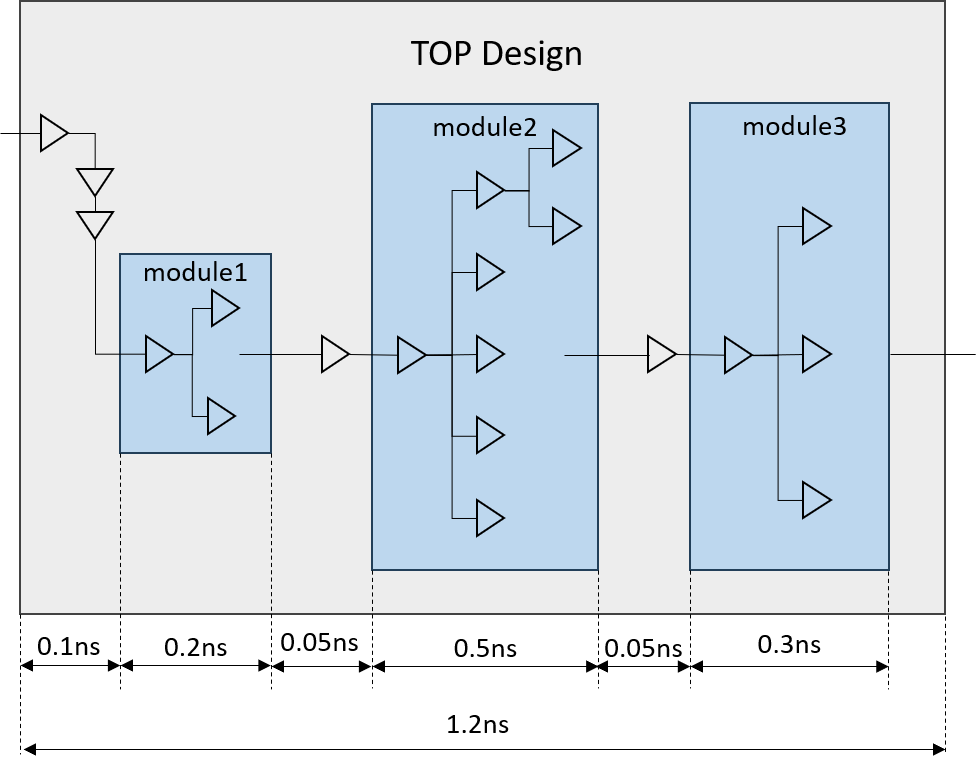
\includegraphics[width=0.8\linewidth]{assets/17/布局规划考虑时钟树延时.png}
  \caption{层次化设计中的布局规划对时钟树延迟的预分配}
  \label{fig:chip-place-time}
\end{figure}

\subsection{电源规划}\label{sec:17-chip-backend-005}

电源规划的简单原理是为芯片中的各个元件提供稳定的电源供应。芯片中的各个元件需要不同的电源电压和电流，因此需要设计合理的电源网络来满足这些需求。电源规划的基本设置包括确定电源电压、电流需求，设计电源网格等。

电源网格是由金属线组成的网络，用于将电源从电源引脚传输到芯片中的各个元件。电源网格的设计需要考虑到电流密度、电压降等因素，以确保电源供应的稳定性。例如，对于高性能的处理器芯片，需要设计密集的电源网格，以满足大电流的需求；同时，需要控制电源网格的电阻和电感，以减少电压降和噪声。

\subsection{自动布局和时序、功耗、面积优化}\label{sec:17-chip-backend-006}

自动布局是利用EDA工具自动将标准单元放置在芯片中的合适位置。在前面手动完成布局规划之后，由EDA工具考虑时序、功耗、面积等因素优化完成自动布局任务。自动布局可以提高设计效率，减少人工干预，同时也可以提高设计的质量和可靠性。

时序优化的目的是确保芯片的时序性能满足设计要求。基本设置包括设置时序约束、调整时钟树结构等。时序优化可以通过调整布局、布线、时钟树等方式来实现。例如，可以通过调整标准单元的位置和方向，减少信号传输的延迟；可以通过调整时钟树的结构和延迟，减少时钟偏移和抖动。

功耗优化的方法包括降低电压、减少开关活动等。功耗优化可以通过调整电源电压、优化电路设计、减少不必要的开关活动等方式来实现。例如，可以通过降低电源电压，减少静态功耗；可以通过优化电路设计，减少动态功耗。

面积优化可以通过压缩布局、优化布线等方式实现。面积优化可以减少芯片的面积，降低成本，同时也可以提高芯片的性能和可靠性。例如，可以通过压缩标准单元的布局，减少芯片的面积；可以通过优化布线，减少布线长度和交叉，提高信号传输的质量。

上述优化一般由EDA工具辅助完成。

\subsection{时钟树综合}\label{sec:17-chip-backend-007}

时钟树综合是构建时钟信号的传输网络，确保时钟信号的准确性和稳定性。时钟树综合工具会将某个同步设计中的时钟信号到达各个终端节点的时间相同，示意图如图\ref{fig:CTS}所示。

\begin{figure}[htbp]
  \centering
  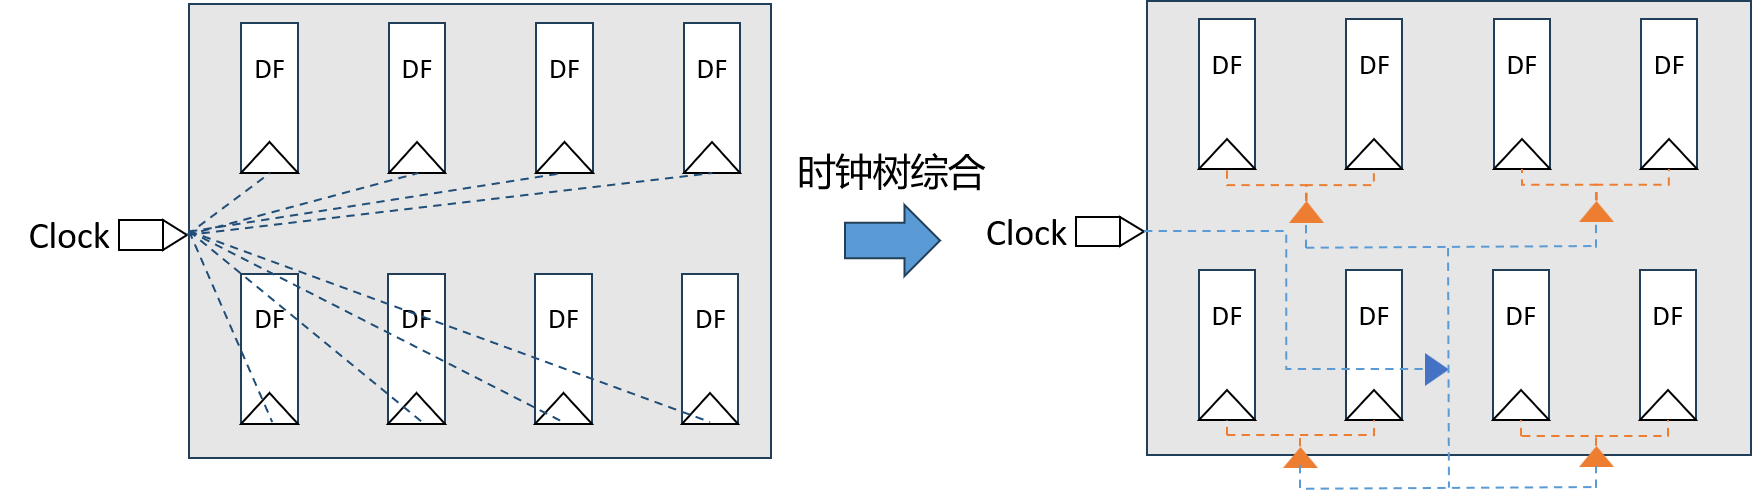
\includegraphics[width=1\linewidth]{assets/17/时钟树综合.png}
  \caption{时钟树综合示意图}
  \label{fig:CTS}
\end{figure}

时钟树综合的基本步骤包括：

确定时钟源和时钟目标。时钟源通常是芯片中的晶振或外部时钟输入，时钟目标是芯片中的各个寄存器和触发器。

设计时钟树结构，如 H 树、鱼骨形等，如上图中就是H树形结构。时钟树结构的选择需要考虑到芯片的面积、功耗、时序等因素。

调整时钟树的延迟和偏差，满足时序约束。时钟树的延迟和偏差需要根据设计约束进行调整，以确保时钟信号的准确性和稳定性。

例如，对于高性能的处理器芯片，需要设计低延迟、低偏差的时钟树结构，以提高时钟信号的准确性和稳定性；同时，需要考虑到时钟树的功耗和面积，避免过度设计。

\subsection{布线}\label{sec:17-chip-backend-008}

布线是连接芯片中的各个元件，实现信号的传输。布线的基本步骤包括：

全局布线：确定信号的大致路径。全局布线通常采用基于 Steiner 树的算法，以最小化布线长度和交叉。

详细布线：精确地连接各个元件。详细布线通常采用基于迷宫算法或 Dijkstra 算法的工具，以确保信号的完整性和稳定性。

布线优化：调整布线的长度、宽度等参数，提高信号传输的质量。布线优化可以通过调整布线的电阻、电容、电感等参数，减少信号传输的延迟和噪声。

例如，对于高速数据传输的芯片，需要进行严格的布线优化，以确保信号的完整性和稳定性；同时，需要考虑到布线的功耗和面积，避免过度设计。

\subsection{数据输出}\label{sec:17-chip-backend-009}

芯片物理设计完成后，需要输出用于制造芯片的 GDSII 文件。GDSII 文件包含了芯片的物理信息，如元件的位置、形状、连接关系等。在输出 GDSII 文件之前，需要进行最后的检查和验证，确保芯片的设计符合制造工艺的要求。

例如，可以使用物理验证工具对 GDSII 文件进行 DRC、LVS、Antenna 检查等，确保芯片的设计没有违反制造工艺的规则；可以使用时序分析工具对芯片的时序性能进行最后的验证，确保芯片的时序性能满足设计要求。

\section{芯片时序 signoff}\label{sec:17-chip-backend-010}

芯片时序 signoff 的流程包括：

提取时序模型：从物理设计中提取出用于时序分析的模型。时序模型通常包括晶体管级模型、门级模型、寄存器传输级模型等。提取时序模型的工具可以采用静态时序分析（STA）工具或动态时序分析（DTA）工具，但由于DTA的时间一般要远大于STA的时间，因此一般选用STA作为分析工具。

进行静态时序分析（STA）：检查芯片的时序性能是否满足设计要求。STA 是一种基于模型的分析方法，它通过分析芯片的逻辑结构和物理实现，预测芯片的时序性能。STA 可以快速地检查大量的时序路径，发现潜在的时序问题。

修复时序违规：如果存在时序违规，需要进行优化以修复违规。时序违规的修复通常采用调整布局、布线、时钟树等方式来实现。例如，可以通过调整标准单元的位置和方向，减少信号传输的延迟；可以通过调整时钟树的结构和延迟，减少时钟偏移和抖动。

生成时序报告：记录时序分析的结果，供设计人员参考。时序报告通常包括时序路径的延迟、时钟偏移、建立时间和保持时间等信息。

检查内容主要包括：

建立时间和保持时间检查：确保数据在时钟信号的上升沿和下降沿能够正确地被锁存。建立时间是指数据在时钟信号上升沿之前必须稳定的时间，保持时间是指数据在时钟信号上升沿之后必须稳定的时间。

时钟偏移检查：检查时钟信号在不同路径上的延迟差异。时钟偏移是指时钟信号在不同路径上的延迟差异，它会影响芯片的时序性能。

路径延迟检查：检查信号在不同路径上的传输延迟。路径延迟是指信号在不同路径上的传输延迟，它会影响芯片的时序性能。

静态时序分析（STA）是一种基于模型的分析方法，它通过分析芯片的逻辑结构和物理实现，预测芯片的时序性能。STA 可以快速地检查大量的时序路径，发现潜在的时序问题。STA 的基本原理是将芯片的逻辑结构和物理实现转化为时序图，然后通过分析时序图中的路径延迟、时钟偏移、建立时间和保持时间等信息，判断芯片的时序性能是否满足设计要求。

\section{芯片功耗与 IR signoff}\label{sec:17-chip-backend-011}

芯片功耗与 IR signoff 的流程包括：

功耗分析：评估芯片的功耗，确定功耗是否满足设计要求。功耗分析的方法通常包括静态功耗分析和动态功耗分析。静态功耗分析分析是指在芯片不工作时的功耗，动态功耗分析是指在芯片工作时的功耗。

IR 分析：检查芯片的电源网格是否能够提供稳定的电源供应。IR 分析是指检查芯片的电源网格的电压降和电流密度是否在允许的范围内。如果电源网格的电压降和电流密度超过了允许的范围，可能会导致芯片的性能下降或失效。

优化功耗和 IR：如果存在问题，需要进行优化以降低功耗和改善 IR。功耗优化的方法包括降低电压、减少开关活动、优化电路设计等。IR 优化的方法包括调整电源网格的结构、增加电源引脚的数量、降低电源网格的电阻等。

生成功耗和 IR 报告：记录分析的结果，供设计人员参考。功耗和 IR 报告通常包括芯片的功耗、电源网格的电压降和电流密度等信息。

基本原理：

功耗分析主要考虑动态功耗和静态功耗。动态功耗是由芯片中的开关活动引起的，静态功耗是由漏电流等因素引起的。IR 分析是检查电源网格的电压降是否在允许的范围内，以确保芯片能够正常工作。动态功耗的计算公式为 P\_dynamic = C * V\^{}2 * f，其中 C 是电容，V 是电压，f 是频率。静态功耗的计算公式为 P\_static = I\_leakage * V，其中 I\_leakage 是漏电流，V 是电压。IR 分析的基本原理是根据欧姆定律，计算电源网格的电阻和电流，然后根据电阻和电流计算电压降。如果电压降超过了允许的范围，需要进行优化以降低电压降。

\section{物理验证}\label{sec:17-chip-backend-012}

DRC（设计规则检查）

DRC 的流程包括：

定义设计规则：根据制造工艺的要求，定义各种设计规则，如最小线宽、最小间距、最大金属密度等。设计规则是制造芯片的基本要求，违反设计规则可能会导致芯片制造失败。

进行 DRC 检查：使用工具对芯片的物理设计进行检查，确保设计符合设计规则。DRC 检查通常采用自动化工具，如 Calibre、Mentor Graphics 的 DRC 工具等。

修复 DRC 违规：如果存在 DRC 违规，需要进行修改以满足设计规则。DRC 违规的修复通常需要调整布局、布线、金属层等，以确保设计符合制造工艺的要求。

基本原理：DRC 检查是为了确保芯片的物理设计能够在制造过程中顺利实现。制造工艺对芯片的尺寸、间距、金属密度等有严格的要求，如果设计违反了这些要求，可能会导致制造失败。例如，最小线宽和最小间距的要求是为了确保金属线之间有足够的空间，避免短路和漏电；最大金属密度的要求是为了确保芯片在制造过程中不会出现过度蚀刻或过度填充的问题。

LVS（版图与原理图一致性检查）

LVS 的流程包括：

提取原理图和版图信息：分别从逻辑设计和物理设计中提取出原理图和版图信息。原理图信息通常包括电路的逻辑连接关系、元件的参数等；版图信息通常包括芯片的物理布局、金属层的连接关系等。可以使用专门的提取工具来完成这一步骤，确保信息的准确性和完整性。

进行 LVS 检查：比较原理图和版图的连接关系，确保它们是一致的。这一步骤通常使用自动化的 LVS 工具，该工具会对原理图和版图中的各个节点、元件进行逐一对比，检查它们的连接关系、属性等是否匹配。如果发现不一致的地方，工具会生成详细的报告，指出具体的问题所在。

修复 LVS 违规：如果存在 LVS 违规，需要进行修改以确保原理图和版图的一致性。根据 LVS 报告中的问题描述，设计人员需要仔细分析违规的原因，并采取相应的措施进行修复。可能需要调整版图布局、修改电路连接或者更新元件参数等。修复完成后，再次进行 LVS 检查，直到所有问题都得到解决。

基本原理：LVS 检查是为了确保芯片的物理设计与逻辑设计是一致的。如果物理设计与逻辑设计不一致，可能会导致芯片的功能错误。在芯片设计过程中，逻辑设计和物理设计是两个不同的阶段，分别由不同的工具和人员进行。由于各种原因，可能会出现逻辑设计与物理设计不一致的情况，例如在布局布线过程中出现错误连接、元件参数设置错误等。LVS 检查通过比较原理图和版图的连接关系，可以及时发现这些问题，并进行修复，从而保证芯片的正确性和可靠性。

Antenna 检查

Antenna 检查的流程包括：

识别天线结构：在物理设计中识别可能存在天线效应的结构。天线效应是指在制造过程中，芯片中的金属线可能会像天线一样收集电荷，导致晶体管的栅极被击穿。一些较长的金属线、未连接到地的金属结构等都可能成为天线结构。可以使用专门的 Antenna 检查工具来识别这些结构。

计算天线比率：计算天线结构的天线比率，判断是否超过允许的范围。天线比率是指天线结构收集的电荷与晶体管栅极电容的比值。如果天线比率超过了允许的范围，就可能导致栅极被击穿。工具会根据制造工艺的要求，计算每个天线结构的比率，并与允许的范围进行比较。

修复 Antenna 问题：如果天线比率超过允许的范围，需要进行修改以降低天线比率。常见的修复方法包括增加接地连接、插入二极管、调整金属层布局等。设计人员需要根据具体情况选择合适的修复方法，并确保修复后的设计满足制造工艺的要求。再次进行 Antenna 检查，直到所有问题都得到解决。

基本原理：在制造过程中，芯片中的金属线可能会像天线一样收集电荷，导致晶体管的栅极被击穿。Antenna 检查是为了确保芯片的物理设计不会引起天线效应，从而保证芯片的可靠性。当芯片在制造过程中暴露在等离子体环境中时，金属线会收集电荷。如果电荷积累到一定程度，就会超过晶体管栅极的耐压能力，导致栅极被击穿。Antenna 检查通过识别可能存在天线效应的结构，并计算天线比率，可以及时发现潜在的问题，并采取相应的措施进行修复，从而避免芯片在制造过程中出现故障。

% !TeX root = ../main.tex
% 原始章节：18-test-and-show.Rmd

\chapter{回片测试与演示}\label{chap:18-test-and-show}

\section{芯片封装与回片测试}\label{sec:18-test-and-show-001}

\subsection{芯片封装}\label{sec:18-test-and-show-002}

集成电路芯片封装(Packaging,PKG)是指利用膜技术及微细加工技术，将芯片及其他要素在框架或基板上布置、粘贴固定及连接，引出接线端子并通过可塑性绝缘介质灌封固定，构成整体立体结构的工艺。此概念称为狭义的封装。更广意义上的``封装''是指封装工程，即将封装体与基板连接固定，装配成完整的系统或电子设备，并确保整个系统综合性能的工程。将以上所述的两个层次封装的含义合并起来，就构成了广义的封装概念。

将基板技术、芯片封装体、分立器件等全部要素，按电子设备整机要求进行连接和装配，实现电子的、物理的功能，使之转变为适用于整机或系统的形式，成为整机装置或设备的工程称为电子封装工程。

集成电路封装的目的，在于保护芯片不受或少受外界环境的影响，并为之提供一个良好的工作条件，以使集成电路具有稳定、正常的功能。封装为芯片提供了一种保护，人们平时所看到的电子设备如计算机、家用电器、通信设备等中的集成电路芯片都是封装好的，没有封装的集成电路芯片一般是不能直接使用的。

通常，芯片封装(Assembly)和芯片制造(IC Fabrication)并不是在同一工厂内完成的。它们可能在同一个工厂的不同生产区域，或在不同的地区，甚至在不同的国家。因此，许多公司将芯片运送到几千公里以外的地方去做封装。

芯片通常在硅片工艺线上进行片上测试，并将有缺陷的芯片打上了记号，通常是打上一个黑色墨点，这样是为后面的封装过程做好准备，在进行芯片贴装时自动拾片机可以自动分辨出合格的芯片和不合格的芯片。

封装流程一般可以分成两个部分：用塑料封装（固封）之前的工艺步骤称为前段操作(FrotEnd Operation),成型之后的工艺步骤称为后段操作(Back End Operation)。在前段工序中，净化级别控制在1000级。在有些生产企业中，成型工序也在净化的环境下进行。但是，由于转移成型操作中机械水压机和预成型品中的粉尘，使得很难使净化环境达到1000级以上的水平。一般来说，随着硅芯片越来越复杂和日益趋向微型化，将使得更多的装配和成型工艺在粉尘得到控制的环境下进行。

现在使用的大部分封装材料都是高分子聚合物，即所谓的塑料封装。塑料封装的成型技术也有许多种，包括转移成型技术(Transfer Molding)、喷射成型技术(Inject Molding)、预成型技术(Pre-Molding),其中转移成型技术使用最为普遍。本章将重点介绍塑料封装的转移成型工艺。

转移成型技术的典型工艺过程如下：将已贴装好芯片并完成芯片互连的框架带置于模具中，将塑料材料预加热(90℃\textasciitilde95℃)，然后放进转移成型机的转移罐中。在转移成型活塞压力之下，塑封料被挤压到浇道中，并经过浇口注入模腔（170℃175℃)。塑封料在模具内快速固化，经过一段时间的保压，使得模块达到一定的硬度，然后用顶杆顶出模块并放入固化炉进一步固化。

归纳起来芯片封装技术的基本工艺流程为：硅片减薄、硅片切割、芯片贴装、芯片互连、成型技术、去飞边毛刺、切筋成型、上焊锡、打码等工序。

\textbf{实践过程中}，我们一般需要向封装公司提交封装信息评估表：

\begin{itemize}
\tightlist
\item
  芯片的基本信息，例如晶圆大小、晶圆厚度和封装类型等
\item
  Pad与Pin对应关系，即硅片上Pad与封装后芯片引脚的对应关系
\end{itemize}

\subsection{回片测试}\label{sec:18-test-and-show-003}

芯片回片测试是确保半导体产品质量和性能的关键一步。它需要严格的测试流程、专业的测试工具和仔细的数据分析。只有通过有效的回片测试，才能确保芯片在各种应用领域中稳定、可靠地运行。

\textbf{准备回片测试}
在进行芯片回片测试之前，需要进行一系列的准备工作，以确保测试的顺利进行：

\begin{enumerate}
\def\labelenumi{\arabic{enumi}.}
\tightlist
\item
  制备测试工具： 这包括各种测试仪器和设备，如测试台、测试探针、测试仪器（如示波器、信号发生器）以及自动化测试系统。
\item
  制定测试计划： 制定详细的测试计划，包括测试流程、测试条件、测试参数以及所需的测试数据。
\item
  测试程序编写： 编写用于执行测试的自动化测试程序，以确保测试的准确性和可重复性。
\item
  温度控制： 一些芯片需要在特定温度下进行测试，因此需要建立温度控制系统，以模拟实际应用条件。
\end{enumerate}

\textbf{进行回片测试}
芯片回片测试通常包括以下几个关键步骤：

\begin{enumerate}
\def\labelenumi{\arabic{enumi}.}
\tightlist
\item
  电性能测试： 这是最常见的测试步骤之一，用于评估芯片的电气特性。它包括测量输入输出电压、电流、功耗等参数，以确保芯片在不同工作条件下都能正常运行。
\item
  功能测试： 在这个步骤中，对芯片的各个功能模块进行测试，以验证其是否按照设计规格正常工作。这包括数字逻辑、模拟电路、通信接口等功能的验证。
\item
  时序测试： 时序测试用于确保芯片的各个信号在正确的时间点上升或下降。这对于高速通信和时序敏感的应用至关重要。
\item
  温度测试： 对于需要在不同温度下工作的芯片，温度测试是必要的。它可以帮助评估芯片在不同环境条件下的性能。
\item
  可靠性测试： 这些测试包括热应力测试、温度循环测试、静电放电测试等，用于评估芯片的可靠性和稳定性。
\item
  通信性能测试： 对于通信芯片，通信性能测试用于验证芯片与其他设备的通信性能，确保数据传输的准确性和可靠性。
\end{enumerate}

\textbf{数据分析与报告}
在完成回片测试后，需要对测试结果进行详细的数据分析。这包括：

\begin{enumerate}
\def\labelenumi{\arabic{enumi}.}
\tightlist
\item
  数据处理： 对测试数据进行整理、筛选和处理，以便进一步分析。
\item
  结果比对： 将测试结果与设计规格进行比对，查找任何偏差或异常。
\item
  问题识别： 如果测试结果显示问题或不符合规格，需要识别问题的根本原因。
\item
  修复建议： 提供可能的修复建议，以改进芯片的性能和品质。
\item
  生成测试报告： 最终生成详细的测试报告，记录测试过程、结果、问题和解决方案。这个报告通常会被用于产品质量控制、客户沟通和质量改进。
\end{enumerate}

\textbf{修复和再测试}
如果测试发现了问题，芯片可能需要进行修复。修复通常涉及修改掩膜、调整电路设计或更换元件。修复后，再次进行回片测试，以确保问题已解决。这个过程可能需要多次迭代，直到芯片满足设计规格。

\section{测试PCB设计与制作}\label{sec:18-test-and-show-004}

测试PCB（印刷电路板）的设计和制造是芯片测试的关键部分。这个专用的PCB用于承载待测芯片，同时提供必要的电源、信号和数据接口。设计测试PCB时，需要考虑到芯片的所有电气需求和测试方案。这包括为芯片提供适当的电源电压、信号完整性考虑以及接口布局优化，以确保在测试过程中可靠地传输数据和信号。当然有关PCB设计和相关工具使用的内容并不是本文的重点，读者若希望进一步了解这部分内容可以观看\href{https://space.bilibili.com/88050003/channel/collectiondetail?sid=1952366}{【芯片测试】测试电路板设计}系列视频。

\section{完整的芯片测试系统集成}\label{sec:18-test-and-show-005}

\hspace{0pt} 构建完整的芯片测试系统是一个复杂的过程，涉及到硬件和软件的集成。测试系统不仅包括物理接口，如测试PCB和相关的连接设备，还包括软件工具用于控制测试流程、收集数据和分析结果。集成这些组件时，必须确保系统的每个部分都能协同工作，从而实现高效和准确的测试。这通常涉及到测试设备与计算机系统的接口设计，以及开发定制的测试软件，用于自动化测试序列和结果分析。

\textbf{芯片测试板}

在生产环境中进行芯片测试需要构建一个系统。该系统是在一般是在测试板上实现的，该测试板与最终使用该芯片的产品的电路板非常相似。测试板一般包括以下功能和特性:

\begin{enumerate}
\def\labelenumi{\arabic{enumi}.}
\tightlist
\item
  与待测芯片相匹配的引脚底座（实际产片则可直接焊接芯片）
\item
  可放在测试板上的所有待测芯片外设,包括：

  \begin{itemize}
  \tightlist
  \item
    PMIC：Power Management Integrated Circuit，电源管理集成电路
  \item
    DRAM：动态随机存储器（dynamic random-access memory, DRAM），又称动态RAM，是一种半导体存储器，通常被用作主存储器，用于存储运行中的程序和数据。
  \item
    非易失性存储器：如 NVMe/SATA硬盘、eMMC、SD卡等。
  \item
    其他外设或接口：如 USB、网卡、UART等
  \end{itemize}
\item
  仿真电路和回环，用于无法放在测试板上的外设，例如人机接口设备(HID)和 HDMI，在下图中用 \textbf{Mock I/O} 模块表示
\item
  测试用处理器（一般在待测芯片不是通用处理器的情况下使用）
\item
  测试设备和测试用处理器之间的通信方式
\item
  终端应用中使用的系统软件
\end{enumerate}

\textbf{芯片测试机}

连接到测试板时，测试设备至少需要提供以下功能和特性：

\begin{itemize}
\tightlist
\item
  测试板和待测芯片的电源
\item
  与测试用处理器或待测芯片的交互方式
\end{itemize}

更为先进的测试设备还具有以下功能和特性：

\begin{enumerate}
\def\labelenumi{\arabic{enumi}.}
\tightlist
\item
  连接到嵌入式处理器控制台的UART接口，用于实现设备间的通信
\item
  JTAG，用于直接访问待测芯片。功能类似STM32的JTAG接口，通过该接口可实现程序的烧录和单步调试等功能。
\item
  串行外设接口SPI，用于访问测试板上的功能
\item
  高速串行接口，如PCIe、以太网或USB
\item
  自动温度控制
\item
  测试板上闪存设备的自动更新
\end{enumerate}

除了具备以上所说的硬件功能以外，测试设备还必须提供一个计算机平台（测试用PC）和相应的API，以便测试程序访问这些功能和特性。在我们的设计实践中，完整的测试平台一般如图\ref{fig:sys-level-test}所示。

\begin{figure}[htbp]
  \centering
  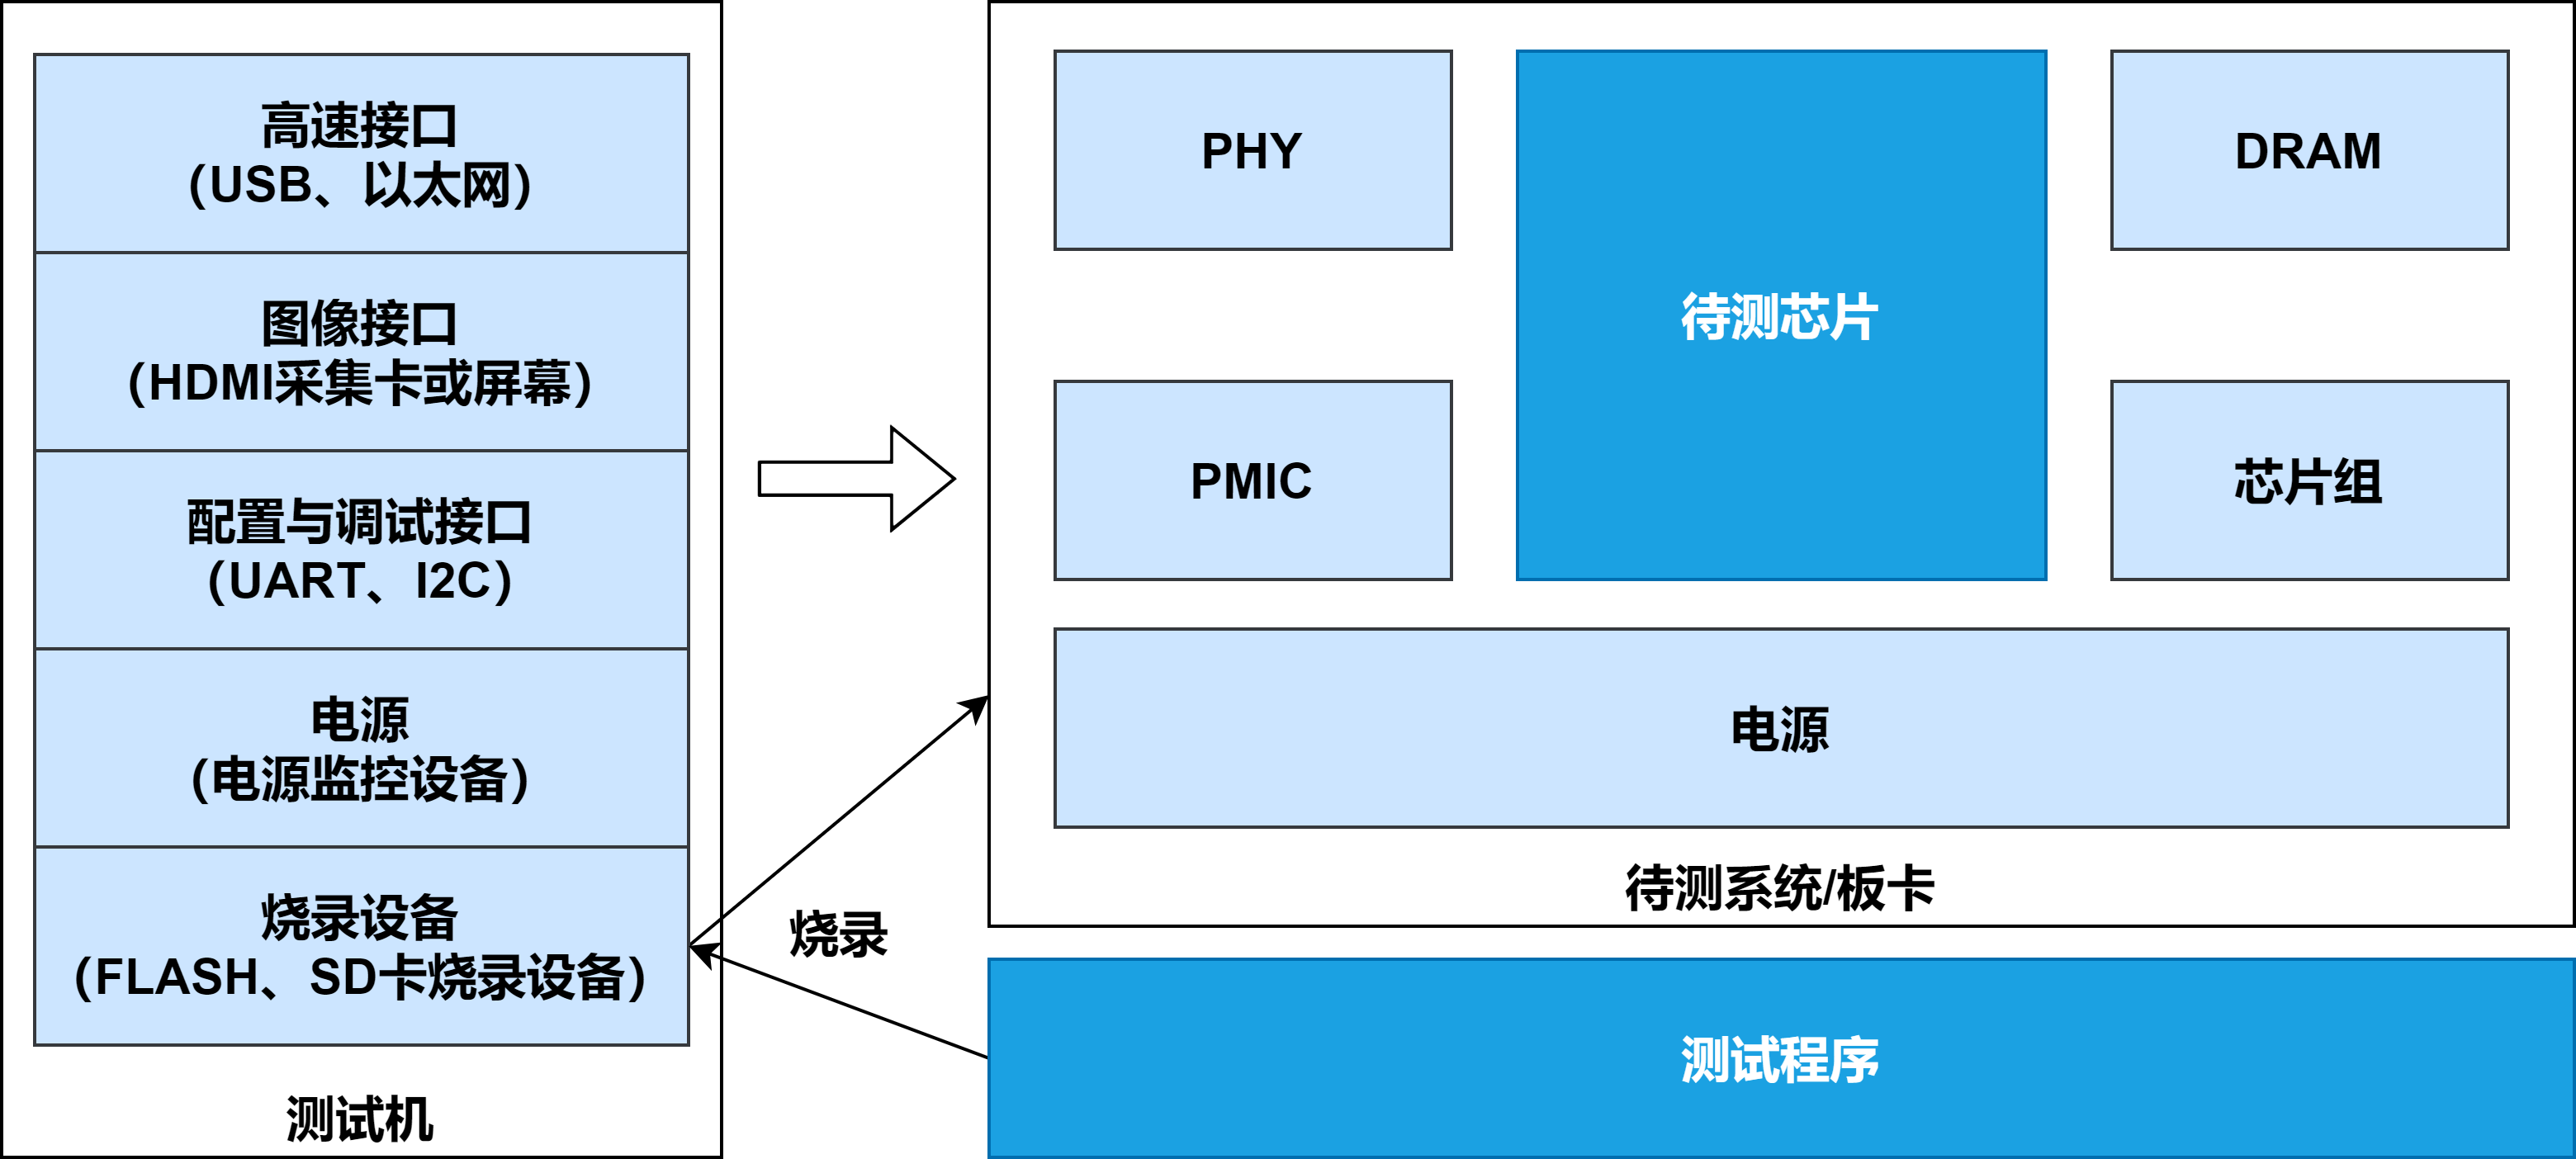
\includegraphics[width=1\linewidth]{assets/18/sys_level_test.png}
  \caption{SoC芯片测试系统}
  \label{fig:sys-level-test}
\end{figure}

\section{性能测试}\label{sec:18-test-and-show-006}

性能测试专注于评估芯片的速度、功耗和总体效率。在这个阶段，测试团队会通过一系列严格的测试来衡量芯片的性能指标，如处理速度、响应时间和功耗等。这些测试帮助识别可能的性能瓶颈和优化点。
性能测试对于确保芯片满足其市场和应用的要求至关重要，特别是对于高性能或低功耗应用的芯片。

对于处理器芯片，业内常使用 SPEC 套件对处理器进行测试。但需要注意的是，SPEC2006 套件及更新，需要至少 1G 的运行内存才可以正常工作，对于小于 1G 的设备，可以考虑使用 SPEC2000 或者其它嵌入式的性能测试工具。

对于嵌入式场景的处理器芯片，常用的测试工具包括 Coremark、Dhrystone 等。对其进行交叉编译，并在处理器芯片上运行即可。没有什么可以特别说明的。


\backmatter
% !TeX root = ../main.tex
% 原始章节：19-conclusion.Rmd

\chapter*{总结}\label{chap:19-conclusion}
\addcontentsline{toc}{chapter}{总结}

\markboth{总结}{总结}

《面向LoongArch国产自主指令集的CPU设计实践》是一本系统介绍LoongArch自主指令集架构下的CPU设计与实现的实践指南。书中的内容不仅涉及处理器设计的理论基础，还深入探讨了从数字电路设计到FPGA验证，再到SoC集成的具体实现过程。本书的完成不仅是我校多年教学、实践和研究工作的结晶，更是希望为广大的师生朋友在国产自主指令集LoongArch发展过程中提供一个重要的学习和参考工具。

\textbf{第一章：CPU芯片设计概述}

本章通过介绍现代计算机系统的基本结构和基本的芯片实现流程，帮助读者了解CPU设计实现的核心概念。本章简要回顾了冯·诺依曼结构、现代SoC架构的发展，阐述了LoongArch架构的背景和重要性并介绍了芯片实现的整体流程。通过这一章节，读者能够掌握CPU设计的基本框架，为后续章节的深入学习打下基础。

\textbf{第二章至第四章：设计环境与基础知识}

本书的第二章到第四章详细介绍了芯片设计开发的硬件、软件环境以及数字逻辑设计的基本流程。第2章侧重于硬件设计和验证环境的搭建，特别介绍了FPGA的相关知识；第3章深入探讨了数字逻辑电路的组成与设计，包括组合逻辑电路和时序逻辑电路的区别与设计方法。第4章则进一步通过具体的设计案例，介绍了LoongArch指令集精简版（LA32R）的处理器开发流程，使读者在进行CPU设计之前，能够熟悉设计工具和方法。这些章节为读者搭建了理论和工具平台，帮助其理解如何在FPGA环境中实现LoongArch CPU的开发。这些内容不仅适用于LoongArch，也为读者在其他硬件设计项目中的开发奠定了基础。

\textbf{第五章至第六章：简单CPU设计与指令扩展}

从第五章开始，书籍进入了LoongArch CPU的核心设计部分。首先，作者通过单周期和流水线设计，逐步引导读者实现一个简单的LA32R CPU。书中不仅介绍了如何设计这些处理器核心，还详细描述了处理流水线冲突、增加Cache、以及优化性能的具体方法。第六章进一步扩展了指令集，介绍了如何在流水线中添加更多的运算类、访存类指令，丰富了处理器的功能。

\textbf{第七章至第九章：中断、异常与SoC集成}

这几章内容对复杂的系统设计进行了详细探讨，包括异常和中断的处理机制、总线接口设计、以及SoC集成。尤其是在第8章和第9章中，作者详细介绍了如何将设计的CPU核集成到更大的SoC系统中，并通过总线协议（如SRAM和AXI）与外部设备进行通信。这些章节帮助读者了解如何设计可扩展的CPU核，并将其整合到一个完整的计算机系统中。通过这些章节，读者不仅能掌握LoongArch CPU设计的核心技术，还能理解如何在SoC环境中集成和调试处理器，进而实现一个完整的嵌入式系统或复杂的计算系统。

\textbf{第十章至第十四章：TLB、MMU设计与操作系统支持}

第十章介绍了TLB和MMU的设计原理和实现细节，重点介绍了如何在处理器中实现虚拟地址转换，确保处理器能够支持现代操作系统的运行。第十一章进一步讨论了如何进一步提升处理器的性能。完成处理器设计后，第十二章介绍了如何在FPGA的环境下对处理器进行验证。第十三章和十四章还探讨了操作系统在处理器上的移植方法，包括如何为LoongArch处理器移植AM系统、启动Linux操作系统等。

\textbf{第十五章至第十八章：芯片实现与验证}

本书的最后几章聚焦于芯片的物理实现和测试环节，涵盖了从前端设计到后端物理设计的完整流程。第16章和第17章介绍了如何通过EDA工具进行逻辑综合、时序分析、功耗与物理验证。最后的章节还描述了芯片的封装与回片测试流程。这些章节为整个书籍提供了完整的闭环，展示了如何将LoongArch CPU从设计概念转化为实际的硬件，并在FPGA板上进行验证和测试。读者不仅能掌握如何设计LoongArch CPU，还能学习如何在物理层面优化设计，确保其在实际应用中的性能和可靠性。

展望未来，随着LoongArch指令集的不断发展和完善，我相信本书所涵盖的内容将继续为更多的学术研究者和工程师提供有价值的参考。同时，我们也期待LoongArch能够在更多的实际应用中发挥更大的作用，为我国的自主计算机系统建设做出更大的贡献。

再次感谢所有在这本书的撰写过程中给予我们帮助的单位和个人！

% !TeX root = ../main.tex
% 原始章节：30-references.Rmd

\chapter*{参考文献}\label{chap:30-references}
\addcontentsline{toc}{chapter}{参考文献}

\markboth{参考文献}{参考文献}

{[}1{]} 汪文祥 邢金璋. CPU设计实战：LoongArch版{[}EB/OL{]}. 2023-11-02{[}2024-8-23{]}. \url{https://bookdown.org/loongson/_book3/}.

{[}2{]} ARM. AMBA AXI and ACE Protocol Specification{[}EB/OL{]}. {[}2024-9-10{]}. \url{https://developer.arm.com/documentation/ihi0022/e}.

{[}3{]} 余子濠. ``一生一芯''学习讲义{[}EB/OL{]}. {[}2024-08-10{]}. \url{https://ysyx.oscc.cc/docs/2306/preliminary/preliminary.html}.

{[}4{]} 深开鸿. \# loongarch架构介绍\# {[}四{]} TLB异常处理{[}EB/OL{]}. 2023-2-17{[}2024-08-06{]}. \url{https://ost.51cto.com/posts/21259}.

{[}5{]} 龙芯中科技术股份有限公司. 龙芯架构32 位精简版参考手册{[}EB/OL{]}. 2023-04{[}2024-08-06{]}. \url{https://www.loongson.cn/uploads/images/2023041918122813624.\%E9\%BE\%99\%E8\%8A\%AF\%E6\%9E\%B6\%E6\%9E\%8432\%E4\%BD\%8D\%E7\%B2\%BE\%E7\%AE\%80\%E7\%89\%88\%E5\%8F\%82\%E8\%80\%83\%E6\%89\%8B\%E5\%86\%8C_r1p03.pdf}.

{[}6{]} 姚永斌. 超标量处理器设计{[}M{]}. 2014年4月第一版. 清华大学出版社, 2014.

{[}7{]} zhangxi. CHIPLAB使用介绍{[}EB/OL{]}. {[}2024-08-07{]}. \url{https://chiplab.readthedocs.io/}.

{[}8{]} Readon. Spinal Hardware Description Language{[}EB/OL{]}. {[}2024-08-08{]}. \url{https://spinalhdl.github.io/SpinalDoc-RTD/master/index.html}.

{[}9{]} AMD. Clocking Wizard{[}EB/OL{]}. {[}2024-08-09{]}. \url{https://www.xilinx.com/products/intellectual-property/clocking_wizard.html}.

{[}10{]} TrustZone\_Hcoco. 芯片测试：系统级测试（SLT）详解{[}EB/OL{]}. {[}2024-08-10{]}. \url{https://blog.csdn.net/weixin_45264425/article/details/134082293}.

{[}11{]} 赵子豪. LoongArch处理器芯片物理后端设计与实现{[}D{]}. 北京航空航天大学: 北京航空航天大学, 2024.

{[}12{]} 成晨. 面向国产LoongArch处理器芯片的可测试性设计{[}D{]}. 北京航空航天大学: 北京航空航天大学, 2024.

{[}13{]} 苏阳. LoongArch处理器芯片设计实现与系统开发{[}D{]}. 北京航空航天大学: 北京航空航天大学, 2024.

{[}14{]} 王哲. 基于LoongArch指令集的多核处理器设计与实现{[}D{]}. 北京航空航天大学: 北京航空航天大学, 2024.

{[}15{]} 郭骐鸣. 基于LoongArch的操作系统内核设计与实现{[}D{]}. 北京航空航天大学: 北京航空航天大学, 2024.

{[}16{]} 郭鸿宇. 面向LoongArch指令集的体系结构模拟器设计与实现{[}D{]}. 北京航空航天大学: 北京航空航天大学, 2024.

{[}17{]} 周振源. 基于LoongArch指令集的乱序超标量处理器设计及软件应用开发{[}D{]}. 北京航空航天大学: 北京航空航天大学, 2024.

{[}18{]} 胡伟武 汪文祥 苏孟豪 张福新 王焕东 章隆兵 肖俊华 刘 苏 陈新科 吴瑞阳 李晓钰 高燕萍. 计算机体系结构基础{[}EB/OL{]}. 2023-09-14{[}2024-08-08{]}. \url{https://foxsen.github.io/archbase/}.

{[}19{]} Jevon. 超标量处理器学习笔记{[}EB/OL{]}. 2020-06-18{[}2024-08{]}. \url{https://www.zhihu.com/column/c_1253708282457079808}.

{[}20{]} 李可为. 集成电路芯片封装技术{[}M{]}. 第二版. 电子工业出版社, 2013.

% !TeX root = ../main.tex
% 原始章节：40-resources.Rmd

\chapter*{相关资料}\label{chap:40-resources}
\addcontentsline{toc}{chapter}{相关资料}

\markboth{相关资料}{相关资料}

\begin{longtable}[]{@{}
  >{\raggedright\arraybackslash}p{(\linewidth - 4\tabcolsep) * \real{0.0741}}
  >{\raggedright\arraybackslash}p{(\linewidth - 4\tabcolsep) * \real{0.3704}}
  >{\raggedright\arraybackslash}p{(\linewidth - 4\tabcolsep) * \real{0.5556}}@{}}
\toprule\noalign{}
\begin{minipage}[b]{\linewidth}\raggedright
章节序号
\end{minipage} & \begin{minipage}[b]{\linewidth}\raggedright
名称
\end{minipage} & \begin{minipage}[b]{\linewidth}\raggedright
链接
\end{minipage} \\
\midrule\noalign{}
\endhead
\bottomrule\noalign{}
\endlastfoot
2.3.2 & 虚拟机获取链接 & \url{https://pan.baidu.com/s/1CRMtk3d95JQnBx6FbHBWXA?pwd=chip} \\
2.3.4 & 北航龙架构处理器芯片敏捷设计框架（BHLA） & \url{https://github.com/BUAA-CI-LAB/BHLA.README} \\
2.3.4 & 龙芯教育提供的相关资料 & \url{https://gitee.com/loongson-edu} \\
4.3.2 & 南京大学 AM & \url{https://github.com/NJU-ProjectN/abstract-machine.git} \\
4.3.2 & 南京大学 NEMU & \url{https://gitee.com/wwt_panache/la32r-nemu.git} \\
14.3 & BusyBox 官方 Git 镜像仓库 & \url{https://github.com/mirror/busybox} \\
15.1.2 & Clocking Wizard IP官方文档 & \url{https://www.xilinx.com/products/intellectual-property/clocking_wizard.html} \\
15.1.4 & SpinalHDL Sdram库链接 & \url{https://github.com/SpinalHDL/SpinalHDL/tree/dev/lib/src/main/scala/spinal/lib/memory/sdram} \\
18.2 & 【芯片测试】测试电路板设计 & \url{https://space.bilibili.com/88050003/channel/collectiondetail?sid=1952366} \\
\end{longtable}

\end{document}
